\documentclass[doctor,twoside,openright,notchinese]{ustcthesis}
% 默认twoside 双面打印
% 将master修改为bachelor, doctor or master
% 要使用adobe字体,添加adobefonts选项
% 要使用Mac系统的字体,添加macfonts选项
% 使用euler数学字体,如不愿使用,去掉euler
% 使用外文写作,请添加notchinese

% 设置图形文件的搜索路径
\graphicspath{{figures/}}

%仅用于本示例文档中显示特殊字符串
\usepackage{xltxtra}
\usepackage{rotating,makecell}
\usepackage{dcolumn}

%%%%%%%%%%%%%%%%%%%%%%%%%%%%%%
%% 封面部分
%%%%%%%%%%%%%%%%%%%%%%%%%%%%%%

  % 中文封面内容
  \title{RHIC能区铀核铀核对撞中双轻子产生}%一般情况下扉页和封皮、书脊共用一个标题文本,可以不用定义\spinetitle(仅硕博有用), \covertitle(本硕博均有用)和\encovertitle(仅本科有用)。特殊情况见下。
 \spinetitle{\small{\raisebox{-3.5pt}{RHIC} 能区铀核铀核对撞中双轻子产生}}
  %特殊情况1:本例中\title命令里含有换行控制字符,这会导致制作书脊的时候出现错误,例如如果你注释掉\spinetitle{...}这一行就会报错。这时需要定义一个不含换行等命令的\spinetitle,这并不表示\spinetitle里不能有任何命令——只能使用有限的命令。
  %特殊情况2:本例中标题过长,所以需要缩小书脊标题的字号。
  %特殊情况3:本例中中英文混排,由于tex竖排的原理限制,中英文基线不重合,所以需要人工调整英文的基线。具体调整量根据不同字体有所不同。
  %\covertitle{相对论重离子对撞机上 $\sqrt{s_{NN}}$ = 193 GeV 铀铀对撞中双轻子的测量}
  %\covertitle{中文题目第一行\\中文题目第二行}
  %不要在此调整封皮字体大小! Do not set Cover Page font size here!
  %特殊情况4:本例中\title中含有多个换行,导致标题超过了两行。根据制本厂规定,封皮标题不能超过两行。因此需要定义封皮使用的标题\covertitle. 如果你注释掉这一行,就会发现封皮不符合规定。

  \author{杨\ 帅}
  \depart{四系}%系别,硕博请用系代号
  \major{粒子物理与原子核物理}%专业,硕博请用全称,本科不需要
  \advisor{李\ 澄\ 教授}
  \coadvisor{阮丽娟\ 研究员}%第二导师
  \submitdate{二〇一六年五月}

  % 英文封面内容
  \entitle{Dielectron production in U + U collisions at $\sqrt{s_{NN}}$ = 193 GeV\\at RHIC}
  \enauthor{Shuai Yang}
  \enmajor{Particle and Nuclear Physics}
  \enadvisor{Prof. Cheng Li}
  \encoadvisor{Prof. Lijuan Ruan}%第二导师
  \ensubmitdate{May, 2016}
  
\begin{document}

  % 封面
  \maketitle

%特别注意,以下述顺序为准,在对应部分添加文档部件,切勿颠倒顺序:
%本科论文的文档部件顺序是:
%    frontmatter:致谢、目录、中文摘要、英文摘要、
%    mainmatter: 正文章节
%    backmatter: 参考文献或资料注释、附录
%硕博论文的文档部件顺序是:
%    frontmatter:中文摘要、英文摘要、目录、符号说明
%    mainmatter: 正文章节
%    backmatter: 参考文献、附录、致谢、发表论文
%%%%%%%%%%%%%%%%%%%%%%%%%%%%%%
%% 前言部分
%%%%%%%%%%%%%%%%%%%%%%%%%%%%%%
\frontmatter
\makeatletter
\ifustc@bachelor
	%%%%%%%%%%%%%%%%%
	%本科论文修改这里
	%%%%%%%%%%%%%%%%%
	% 致谢
	\begin{thanks}

This thesis could never come out without the support and help from lots of people. I would like to express my gratitude to these listed in the following and many others I might not mention.

First of all, I would thank Prof. Cheng Li, who has been my adviser since I was a undergraduate student. He introduced me to this field and provided the great opportunity to participate the BES\uppercase\expandafter{\romannumeral3} eTOF upgrade and the STAR MTD programs. I appreciate his continuous supervision and support in the last seven years. My gratitude also goes to Prof. Lijuan Ruan who is the co-advisor of my PhD research. She guided me all the analysis details throughout the thesis. I am impressive by her numerous ideas and enthusiasm on the research. I have benefited so much from the day-to-day discussion with her in the last three and half years. I would like to thank Prof. Zhangbu Xu for offering the opportunity to study at BNL, the wonderful place for relativistic heavy-ion physics research. He also guided me the details of THGEM related work and helped me a lot in my analysis. I have learned a lot from the tons of fruitful discussions with him. I also appreciate Prof. Hongfang Chen for her support and encouragement. She, as a scientist and a mentor, sets an example to young people.

My special thanks goes to Prof. Zebo Tang, who introduced me to the heavy-ion physics filed. He guided me the cosmic ray analysis at the very beginning, which started my STAR journey. He always answers my questions with patience no matter how silly they may have been. My special thanks also goes to Dr. Bingchu Huang who taught me a lot in my analysis, MTD related works and lots of technical skills. He also helped me a lot on my living at BNL. I would like to express my gratitude to Dr. Yongjie Sun who guided me on manufacturing and testing MRPC modules.

I would like to thank Dr. Wangmei Zha, and Dr. Chi Yang for pleasant cooperation on installing and commissioning MTD system and lots of helpful discussions on physics and other things. I would like to thank Dr. Hongwei Ke who taught me a lot on coding and understanding STAR software. I also would like to thank Dr. Yi Guo for his discussions and assistances in my analysis. I would like to thank Yifei Xu and Jinlong Zhang, my roommates at BNL, for enjoyable corporation on work, living and abundant helpful discussions. 

I would like to thank the MTD group, dielectron group, light flavor physics working group in STAR Collaboration, especially Dr. Rongrong Ma, Dr. Takahito Todoroki, Prof. Xin Dong, Prof. Frank Geurts, Joey Butterworth and Liwen Wen. I appreciate many assistances from the High Energy Physics Group at USTC, especially Prof. Zizong Xu, Prof. Xiaolian Wang, Prof. Ming Shao, Prof. Qun Wang, Prof. Yifei Zhang, Dr. Yi Zhou, Dr. Tianxiang Chen, Hui Zhang, Kun Jiang, Yuxiang Zhao, Lailin Xu, Xiaozhuang Wang, Yinying Zhu, Rongxing Yang, Wenhao You, Xiaokun Zhao, Shenghui Zhang, and Guannan Xie. I also would like to thank Dr. Xiangli Cui, Dr. Liang Zheng, Dr. Xueye Hu, Dr. Qiye Shou, Qian Yang, Long Zhou, Zhengqiao Zhang, Xiaoxuan Chu, Zhen Liu, Zaochen Ye, Bo Gao, Xinjie Huang, Zhao Feng, Xu Wang, and Chensheng Zhou. We live at BNL like a family and our life is full of happiness every day. I also would like to express my thanks to non-group member Chenshuo Fu and Zhe Zhou for their friendship and joyful memories together.

Finally, I express my deep gratitude to my dear family. I would like to thank my parents for their selfless dedication, infinite love and unconditional support.  I would not be where I am today without them. I would like to thank my wife, Ying He, who has supported and encouraged me all the time. I am forever thankful for her great understanding. I would like to thank my sister for her continuous support and understanding.
\end{thanks}

	
	%目录部分
	%目录
	\tableofcontents
	%默认表格、插图、算法索引名称分别为“表格索引”、“插图索引”和“算法索引”
	%如果需要自行修改lot,lof,loa的名称,请定义
	%\ustclotname{...}
	%\ustclofname{...}
	%\ustcloaname{...}

	% 表格索引
	\ustclot
	% 插图索引
	\ustclof
	%算法索引 
	%如果需要使用算法环境并列出算法索引,请加入补充宏包。
	\ustcloa
	
	% 摘要
	\begin{cnabstract}
量子色动力学是用来描述夸克和胶子间强相互作用的规范场理论。格点量子色动力学预言在高温或高重子化学势的条件下会发生从强子物质到夸克胶子等离子体(QGP)的相变。坐落在美国布鲁克海文国家实验室(BNL)的相对论重离子对撞机(RHIC)是专门用于研究夸克胶子等离子体性质以及量子色动力学相图的实验装置。双轻子不参与强相互作用,并且可以在重离子对撞整个演化过程中产生,因此,双轻子的测量在研究这种高温高密物质中起着至关重要的作用。

根据不同的产生机制,双轻子的不变质量谱一般被划分成三个质量区间。高质量区间 (HMR, $M_{ll}>M_{J/\psi}$), 双轻子主要由初始的硬过程产生,例如 Drell-Yan,夸克偶素的衰变。中间质量区间(IMR, $M_{\phi}<M_{ll}<M_{J/\psi}$), 双轻子主要由夸克胶子等离子体的热辐射以及开粲的半轻子衰变产生,其中热辐射的双轻子产额可用于测量夸克胶子等离子体的温度。低质量区间(LMR, $M_{ll}<M_{\phi}$),双轻子主要由在强子介质中矢量介子($\rho$, $\omega$, $\phi$, 等)的衰变产生, 他们可用于研究介质中的手征对称性恢复。此外,ALICE合作组最近观察到在质心能量为2.76 TeV的铅核-铅核偏心对撞中,超低横动量($p_{T}<$ 0.3 GeV/$c$)的前向快度$J/\psi$产额有非常大的增强。这部分增强有可能来自相干光产生过程。如果在偏心重离子对撞中,也可以通过相干光产生生成$\rho$介子, 这部分$\rho$介子可用作一个直接测量夸克胶子等离子体性质的探针。

本论文利用位于相对论重离子对撞机上的螺旋径迹探测器(STAR),首次研究了双轻子在铀核-铀核对撞中的产生。 用于该分析研究的数据采集于2012年。利用时间投影室测量的电离能损以及飞行时间探测器测量的粒子速度进行正负电子的鉴别。在铀核-铀核的最小无偏对撞中(中心度:0-80\%),鉴别出来的电子整体纯度可以达到95\%。通过对比在最小无偏对撞中测量的STAR接收度内($p_{T}^{e}$ > 0.2 GeV/$c$, $|\eta^{e}|<$ 1, and $|y_{ee}|<$ 1)的双轻子不变质量谱和不包含$\rho$介子贡献的强子衰变模拟(cocktail),我们发现在类$\rho$质量区间0.3-0.76 GeV/$c^{2}$内,测量的双轻子产额比模拟的产额高 2.1 $\pm$ 0.1(stat.) $\pm$ 0.2(sys.) $\pm$ 0.3(cocktail) 倍。我们还系统的测量了不同横动量以及中心度区间的双轻子不变质量谱,发现此增强因子并没有很强的中心度以及横动量依赖性。为了定量的研究这些双轻子增强,我们还测量了修正STAR接收度的双轻子增强谱(data - cocktail)。上面提到的所有双轻子增强谱都可以用一个包含$\rho$展宽的谱函数以及夸克胶子等离子体热辐射贡献的理论模型描述。$\rho$介子谱在高温高密介质中的展宽被认为和手征对称性恢复有关。进一步的分析研究表明,带电粒子密度($dN_{ch}/dy$)归一的修正了STAR接收度的积分增强产额(积分区间:0.4 $<M_{ee}<$ 0.75 GeV/$c^{2}$)有很强的中心度以及对撞能量的依赖性。中心对撞中的归一积分增强产额比偏心对撞以及低能量对撞的产额要高。最近一个理论模型指出,在质心能量为6到200 GeV区间内,$dN_{ch}/dy$归一的积分增强产额正比于重离子对撞中产生介质的寿命。这预示着在铀核-铀核中心对撞中产生的介质的寿命比在偏心对撞中或者低质心能量重离子对撞中产生的介质寿命长。

本论文还首次测量了铀核-铀核对撞中STAR接收度内超低横动量($p_{T}<$ 0.15 GeV/$c$)的双轻子不变质量谱。相对于强子衰变的模拟产额,偏心对撞中的双轻子产额在整个质量区间都有很大的增强。在质量区间0.4 - 0.76 GeV/$c^{2}$和2.8 - 3.2 GeV/$c^{2}$中,增强因子分别为16.4 $\pm$ 1.1(stat.) $\pm$ 2.6(sys.) $\pm$ 4.2(cocktail),20.4 $\pm$ 4.2(stat.) $\pm$ 3.0(sys.) $\pm$ 3.2(cocktail)。这些增强可能来自于相干光产生过程。我们还测量了铀核-铀核对撞中STAR接收度内不同质量区间的双轻子横动量谱(0.4 $<M_{ee}<$ 0.76 GeV/$c^{2}$, 1.2 $<M_{ee}<$ 2.67 GeV/$c^{2}$, and 2.8 $<M_{ee}<$ 3.2 GeV/$c^{2}$),发现这些横动量谱的形状在偏心对撞中在0.1 GeV/$c$附近发生急剧变化。

此外,本论文还报告了两种气体探测器-迷你漂移厚气体电子倍增室(mini-drift THGEM)和多气隙阻性板室(MRPC)的研制以及测试结果。THGEM用作穿越辐射探测器(TRD)的读出探测器,用来鉴别电子离子对撞机上的前向散射电子和提供额外的电离能损($dE/dx$)测量,后者对小角度散射的带电粒子径迹重建非常重要。这是首次提出用THGEM作为TRD的读出探测器。宇宙线测试结果表明,在工作电压下,THGEM的探测效率高于94\%, 位置分辨能达到220 $\mu$m。 由于THGEM具有非常好的位置分辨以及相对厚的电离区,THGEM展现出非常卓越的径迹重建能力。 最后,测试结果表明THGEM增益均匀性以及稳定性也非常好。为了提高北京谱仪的粒子鉴别能力,MRPC被用来升级北京谱仪端盖飞行时间探测器(eTOF)。我们在正负电子对撞机E3束流线上用动量为600 MeV/$c$的质子束测试了单端读出和双端读出MRPC。 在工作高压下,两种MRPC的探测效率都高于98\%。单端读出MRPC的时间分辨为47 ps,但有带电粒子入射位置的依赖性。双端读出MRPC的时间分辨为40 ps,且没有带电粒子入射位置的依赖性。根据这次束流测试结果,双端读出MRPC被用于北京谱仪的eTOF升级。北京谱仪的eTOF升级已于2015年11月完成,对电子的时间分辨可达到60 ps,远好于其设计指标(80 ps)。

%\keywords{中国科学技术大学\enskip 学位论文\enskip \LaTeX{}~通用模板\enskip 学士\enskip 硕士\enskip 博士}
\end{cnabstract}

\begin{enabstract}
Quantum Chromodynamics (QCD) is a basic gauge field theory to describe strong interactions, a fundamental force describing the interactions between quarks and gluons. Lattice QCD calculations predict a smooth cross-over transition from hadronic phase to the Quark Gluon Plasma (QGP) phase at high temperature ($T$) and small baryon chemical potential ($\mu_{B}$), and a first order phase transition at large $\mu_{B}$ region. The Relativistic Heavy Ion Collider, located at Brookhaven National Laboratory, is a dedicated machine to study the properties of the QGP and the QCD phase diagram in laboratory. Dileptons are produced in the whole evolution of the system and escape with minimum interaction with the strongly interacting medium. Thus, dilepton measurements play an essential role in the study of hot and dense nuclear matter.

According to different physics interests, the dilepton invariant mass spectrum is typically divided into three regions. The High Mass Region (HMR, $M_{ll}>M_{J/\psi}$ ), in which the dileptons are produced by the initial hard perturbative QCD process (Drell-Yan, quarkonia etc.). The Intermediate Mass Region (IMR, $M_{\phi}<M_{ll}<M_{J/\psi}$), in which the dileptons are expected to be directly related to the thermal radiation of the QGP which can be used to determine the initial temperature of the QGP medium. The Low Mass Region (LMR, $M_{ll}<M_{\phi}$), in which the dilepton production is dominated by the in-medium decay of vector mesons ($\rho$, $\omega$, $\phi$, etc.) which are considered as a link to chiral symmetry restoration. Recently, a significant excess of J/$\psi$ yield at very low $p_{T}$ ($p_{T}<$ 0.3 GeV/$c$) has been observed by the ALICE collaboration in peripheral hadronic Pb + Pb collisions at $\sqrt{s_{NN}}$ = 2.76 TeV at forward-rapidity, which may be related to coherent photoproduction of J/$\psi$. If $\rho$ meson can be produced via coherent photoproduction process in peripheral heavy-ion collisions, it might sit in the QGP before its decay. This provides a direct probe of the QGP.

In this thesis, we report the measurements of dielectron production in U + U collisions at $\sqrt{s_{NN}}$ = 193 GeV at Solenoidal Tracker at RHIC (STAR). The data set used in this analysis was taken in year 2012 (Run12). The electron (positron) can be identified by combing ionization energy loss $dE/dx$ measured by the Time Projection Chamber (TPC) and particle velocity measured by the Time of Flight (TOF). A $\sim$95\% overall electron purity can be achieved in U + U minimum-bias collision (0-80\%) at $\sqrt{s_{NN}}$ = 193 GeV. The measured dielectron invariant mass spectrum within STAR acceptance ($p_{T}^{e}$ > 0.2 GeV/$c$, $|\eta^{e}|<$ 1, and $|y_{ee}|<$ 1) in minimum-bias collisions shows an enhancement with respect to hadronic cocktail simulation in 0.3 $<M_{ee}<$ 0.76 GeV/$c^{2}$ ($\rho$-like). The enhancement factor (data/cocktail), integrated over the $\rho$-like mass region and the full $p_{T}$ acceptance, is 2.1 $\pm$ 0.1(stat.) $\pm$ 0.2(sys.) $\pm$ 0.3(cocktail). Meanwhile, systematic measurements are performed in differential $p_{T}$ and centrality bins. The enhancements in LMR are consistently observed and the enhancement factor has a mild $p_{T}$ or centrality dependence. To quantitatively study the dielectron excess, the acceptance-corrected dielectron excess mass spectrum (data - cocktail) is also performed. These excess spectra can be consistently described by a theoretical model calculation incorporating a broadened $\rho$ spectral function and QGP thermal radiation. The integrated acceptance-corrected excess yield in 0.4 $<M_{ee}<$ 0.75 GeV/$c^{2}$ normalized by charged particle density ($dN_{ch}/dy$), has a strong centrality and collision-energy dependence. Recently, it is found in a model calculation that the $dN_{ch}/dy$ normalized dilepton excess yield in the low mass region is proportional to the lifetime of the hot, dense medium created in heavy-ion collisions at $\sqrt{s_{NN}}$ = 6 - 200 GeV. The $dN_{ch}/dy$ normalized integrated yield of the most central U + U collisions at $\sqrt{s_{NN}}$ = 193 GeV is higher than those in peripheral or lower-energy collisions, which indicates that the hot and dense medium created in central U + U collisions at $\sqrt{s_{NN}}$ = 193 GeV has a longer lifetime.

We also report the dielectron invariant mass spectra within STAR acceptance at very low $p_{T}$ ($p_{T}<$ 0.15 GeV/$c$) in U + U collisions. The dielectron invariant mass spectrum shows a significant enhancement compared to hadronic cocktail for the entire mass region in the most peripheral (60-80\%) collisions. The enhancement factors are 16.4 $\pm$ 1.1(stat.) $\pm$ 2.6(sys.) $\pm$ 4.2(cocktail) and 20.4 $\pm$ 4.2(stat.) $\pm$ 3.0(sys.) $\pm$ 3.2(cocktail) in 0.4 $<M_{ee}<$ 0.76 GeV/$c^{2}$ and 2.8 $<M_{ee}<$ 3.2 GeV/$c^{2}$, respectively. The $p_{T}$ spectra within STAR acceptance for three selected invariant mass regions (0.4 $<M_{ee}<$ 0.76 GeV/$c^{2}$, 1.2 $<M_{ee}<$ 2.67 GeV/$c^{2}$, and 2.8 $<M_{ee}<$ 3.2 GeV/$c^{2}$) are also reported. They have a fairly sharp transition around 0.1 GeV/$c$ in the most peripheral U + U collisions.

In addition, we report a R\&D work on two different gaseous detectors: mini-drift THick Gas Electron Multiplier chamber (THGEM) and Multi-gap Resistive Plate Chamber (MRPC). This kind mini-drift THGEM chamber is proposed as part of a transition radiation detector (TRD) for identifying electrons and providing additional $dE/dx$ measurement which is essential for small angle scattering at an Electron Ion Collider (EIC) experiment. Through a cosmic ray test, an efficiency larger than 94\% and a spatial resolution $\sim$220 $\mu$m are achieved for the THGEM chamber. Thanks to its outstanding spatial resolution and relative thick ionization gap, the THGEM chamber shows excellent track reconstruction capability. The gain uniformity and stability of the THGEM chamber are also presented. The MRPC is used to upgrade the Beijing Spectrometer end-cap Time of Flight (eTOF) to enhance the particle identification capability. Two different MRPC designs, single-end readout and double-end readout, were tested using 600 MeV/$c$ proton beam at the E3 line of Beijing Electron Positron Collider (BEPC\uppercase\expandafter{\romannumeral2}). The efficiencies of these two different kinds of MRPCs are better than 98\%. The time resolution of double-end readout MRPC is 40 ps while that of the single-end readout MRPC is 47 ps. Moreover, the time resolution of double-end readout MRPC has no incident position dependence while that of single-end readout MRPC has. Since the tracking performance is limited in precision within the Beijing Spectrometer eTOF acceptance, the double-end readout MRPC is selected for the eTOF upgrade according to this beam test. In November 2015, the MRPC-based eTOF system was fully installed in Beijing Spectrometer. The time resolution of the MRPC-based eTOF system obtained from the collision data is $\sim$60 ps, which is much better than the design specification (80 ps).

%\enkeywords{University of Science and Technology of China (USTC), Thesis, Universal \LaTeX{} Template, Bachelor, Master, PhD}
\end{enabstract}
%此文件中含有中英文摘要
\else
	%%%%%%%%%%%%%%%%%
	%硕博论文修改这里
	%%%%%%%%%%%%%%%%%
	% 摘要
	\begin{cnabstract}
量子色动力学是用来描述夸克和胶子间强相互作用的规范场理论。格点量子色动力学预言在高温或高重子化学势的条件下会发生从强子物质到夸克胶子等离子体(QGP)的相变。坐落在美国布鲁克海文国家实验室(BNL)的相对论重离子对撞机(RHIC)是专门用于研究夸克胶子等离子体性质以及量子色动力学相图的实验装置。双轻子不参与强相互作用,并且可以在重离子对撞整个演化过程中产生,因此,双轻子的测量在研究这种高温高密物质中起着至关重要的作用。

根据不同的产生机制,双轻子的不变质量谱一般被划分成三个质量区间。高质量区间 (HMR, $M_{ll}>M_{J/\psi}$), 双轻子主要由初始的硬过程产生,例如 Drell-Yan,夸克偶素的衰变。中间质量区间(IMR, $M_{\phi}<M_{ll}<M_{J/\psi}$), 双轻子主要由夸克胶子等离子体的热辐射以及开粲的半轻子衰变产生,其中热辐射的双轻子产额可用于测量夸克胶子等离子体的温度。低质量区间(LMR, $M_{ll}<M_{\phi}$),双轻子主要由在强子介质中矢量介子($\rho$, $\omega$, $\phi$, 等)的衰变产生, 他们可用于研究介质中的手征对称性恢复。此外,ALICE合作组最近观察到在质心能量为2.76 TeV的铅核-铅核偏心对撞中,超低横动量($p_{T}<$ 0.3 GeV/$c$)的前向快度$J/\psi$产额有非常大的增强。这部分增强有可能来自相干光产生过程。如果在偏心重离子对撞中,也可以通过相干光产生生成$\rho$介子, 这部分$\rho$介子可用作一个直接测量夸克胶子等离子体性质的探针。

本论文利用位于相对论重离子对撞机上的螺旋径迹探测器(STAR),首次研究了双轻子在铀核-铀核对撞中的产生。 用于该分析研究的数据采集于2012年。利用时间投影室测量的电离能损以及飞行时间探测器测量的粒子速度进行正负电子的鉴别。在铀核-铀核的最小无偏对撞中(中心度:0-80\%),鉴别出来的电子整体纯度可以达到95\%。通过对比在最小无偏对撞中测量的STAR接收度内($p_{T}^{e}$ > 0.2 GeV/$c$, $|\eta^{e}|<$ 1, and $|y_{ee}|<$ 1)的双轻子不变质量谱和不包含$\rho$介子贡献的强子衰变模拟(cocktail),我们发现在类$\rho$质量区间0.3-0.76 GeV/$c^{2}$内,测量的双轻子产额比模拟的产额高 2.1 $\pm$ 0.1(stat.) $\pm$ 0.2(sys.) $\pm$ 0.3(cocktail) 倍。我们还系统的测量了不同横动量以及中心度区间的双轻子不变质量谱,发现此增强因子并没有很强的中心度以及横动量依赖性。为了定量的研究这些双轻子增强,我们还测量了修正STAR接收度的双轻子增强谱(data - cocktail)。上面提到的所有双轻子增强谱都可以用一个包含$\rho$展宽的谱函数以及夸克胶子等离子体热辐射贡献的理论模型描述。$\rho$介子谱在高温高密介质中的展宽被认为和手征对称性恢复有关。进一步的分析研究表明,带电粒子密度($dN_{ch}/dy$)归一的修正了STAR接收度的积分增强产额(积分区间:0.4 $<M_{ee}<$ 0.75 GeV/$c^{2}$)有很强的中心度以及对撞能量的依赖性。中心对撞中的归一积分增强产额比偏心对撞以及低能量对撞的产额要高。最近一个理论模型指出,在质心能量为6到200 GeV区间内,$dN_{ch}/dy$归一的积分增强产额正比于重离子对撞中产生介质的寿命。这预示着在铀核-铀核中心对撞中产生的介质的寿命比在偏心对撞中或者低质心能量重离子对撞中产生的介质寿命长。

本论文还首次测量了铀核-铀核对撞中STAR接收度内超低横动量($p_{T}<$ 0.15 GeV/$c$)的双轻子不变质量谱。相对于强子衰变的模拟产额,偏心对撞中的双轻子产额在整个质量区间都有很大的增强。在质量区间0.4 - 0.76 GeV/$c^{2}$和2.8 - 3.2 GeV/$c^{2}$中,增强因子分别为16.4 $\pm$ 1.1(stat.) $\pm$ 2.6(sys.) $\pm$ 4.2(cocktail),20.4 $\pm$ 4.2(stat.) $\pm$ 3.0(sys.) $\pm$ 3.2(cocktail)。这些增强可能来自于相干光产生过程。我们还测量了铀核-铀核对撞中STAR接收度内不同质量区间的双轻子横动量谱(0.4 $<M_{ee}<$ 0.76 GeV/$c^{2}$, 1.2 $<M_{ee}<$ 2.67 GeV/$c^{2}$, and 2.8 $<M_{ee}<$ 3.2 GeV/$c^{2}$),发现这些横动量谱的形状在偏心对撞中在0.1 GeV/$c$附近发生急剧变化。

此外,本论文还报告了两种气体探测器-迷你漂移厚气体电子倍增室(mini-drift THGEM)和多气隙阻性板室(MRPC)的研制以及测试结果。THGEM用作穿越辐射探测器(TRD)的读出探测器,用来鉴别电子离子对撞机上的前向散射电子和提供额外的电离能损($dE/dx$)测量,后者对小角度散射的带电粒子径迹重建非常重要。这是首次提出用THGEM作为TRD的读出探测器。宇宙线测试结果表明,在工作电压下,THGEM的探测效率高于94\%, 位置分辨能达到220 $\mu$m。 由于THGEM具有非常好的位置分辨以及相对厚的电离区,THGEM展现出非常卓越的径迹重建能力。 最后,测试结果表明THGEM增益均匀性以及稳定性也非常好。为了提高北京谱仪的粒子鉴别能力,MRPC被用来升级北京谱仪端盖飞行时间探测器(eTOF)。我们在正负电子对撞机E3束流线上用动量为600 MeV/$c$的质子束测试了单端读出和双端读出MRPC。 在工作高压下,两种MRPC的探测效率都高于98\%。单端读出MRPC的时间分辨为47 ps,但有带电粒子入射位置的依赖性。双端读出MRPC的时间分辨为40 ps,且没有带电粒子入射位置的依赖性。根据这次束流测试结果,双端读出MRPC被用于北京谱仪的eTOF升级。北京谱仪的eTOF升级已于2015年11月完成,对电子的时间分辨可达到60 ps,远好于其设计指标(80 ps)。

%\keywords{中国科学技术大学\enskip 学位论文\enskip \LaTeX{}~通用模板\enskip 学士\enskip 硕士\enskip 博士}
\end{cnabstract}

\begin{enabstract}
Quantum Chromodynamics (QCD) is a basic gauge field theory to describe strong interactions, a fundamental force describing the interactions between quarks and gluons. Lattice QCD calculations predict a smooth cross-over transition from hadronic phase to the Quark Gluon Plasma (QGP) phase at high temperature ($T$) and small baryon chemical potential ($\mu_{B}$), and a first order phase transition at large $\mu_{B}$ region. The Relativistic Heavy Ion Collider, located at Brookhaven National Laboratory, is a dedicated machine to study the properties of the QGP and the QCD phase diagram in laboratory. Dileptons are produced in the whole evolution of the system and escape with minimum interaction with the strongly interacting medium. Thus, dilepton measurements play an essential role in the study of hot and dense nuclear matter.

According to different physics interests, the dilepton invariant mass spectrum is typically divided into three regions. The High Mass Region (HMR, $M_{ll}>M_{J/\psi}$ ), in which the dileptons are produced by the initial hard perturbative QCD process (Drell-Yan, quarkonia etc.). The Intermediate Mass Region (IMR, $M_{\phi}<M_{ll}<M_{J/\psi}$), in which the dileptons are expected to be directly related to the thermal radiation of the QGP which can be used to determine the initial temperature of the QGP medium. The Low Mass Region (LMR, $M_{ll}<M_{\phi}$), in which the dilepton production is dominated by the in-medium decay of vector mesons ($\rho$, $\omega$, $\phi$, etc.) which are considered as a link to chiral symmetry restoration. Recently, a significant excess of J/$\psi$ yield at very low $p_{T}$ ($p_{T}<$ 0.3 GeV/$c$) has been observed by the ALICE collaboration in peripheral hadronic Pb + Pb collisions at $\sqrt{s_{NN}}$ = 2.76 TeV at forward-rapidity, which may be related to coherent photoproduction of J/$\psi$. If $\rho$ meson can be produced via coherent photoproduction process in peripheral heavy-ion collisions, it might sit in the QGP before its decay. This provides a direct probe of the QGP.

In this thesis, we report the measurements of dielectron production in U + U collisions at $\sqrt{s_{NN}}$ = 193 GeV at Solenoidal Tracker at RHIC (STAR). The data set used in this analysis was taken in year 2012 (Run12). The electron (positron) can be identified by combing ionization energy loss $dE/dx$ measured by the Time Projection Chamber (TPC) and particle velocity measured by the Time of Flight (TOF). A $\sim$95\% overall electron purity can be achieved in U + U minimum-bias collision (0-80\%) at $\sqrt{s_{NN}}$ = 193 GeV. The measured dielectron invariant mass spectrum within STAR acceptance ($p_{T}^{e}$ > 0.2 GeV/$c$, $|\eta^{e}|<$ 1, and $|y_{ee}|<$ 1) in minimum-bias collisions shows an enhancement with respect to hadronic cocktail simulation in 0.3 $<M_{ee}<$ 0.76 GeV/$c^{2}$ ($\rho$-like). The enhancement factor (data/cocktail), integrated over the $\rho$-like mass region and the full $p_{T}$ acceptance, is 2.1 $\pm$ 0.1(stat.) $\pm$ 0.2(sys.) $\pm$ 0.3(cocktail). Meanwhile, systematic measurements are performed in differential $p_{T}$ and centrality bins. The enhancements in LMR are consistently observed and the enhancement factor has a mild $p_{T}$ or centrality dependence. To quantitatively study the dielectron excess, the acceptance-corrected dielectron excess mass spectrum (data - cocktail) is also performed. These excess spectra can be consistently described by a theoretical model calculation incorporating a broadened $\rho$ spectral function and QGP thermal radiation. The integrated acceptance-corrected excess yield in 0.4 $<M_{ee}<$ 0.75 GeV/$c^{2}$ normalized by charged particle density ($dN_{ch}/dy$), has a strong centrality and collision-energy dependence. Recently, it is found in a model calculation that the $dN_{ch}/dy$ normalized dilepton excess yield in the low mass region is proportional to the lifetime of the hot, dense medium created in heavy-ion collisions at $\sqrt{s_{NN}}$ = 6 - 200 GeV. The $dN_{ch}/dy$ normalized integrated yield of the most central U + U collisions at $\sqrt{s_{NN}}$ = 193 GeV is higher than those in peripheral or lower-energy collisions, which indicates that the hot and dense medium created in central U + U collisions at $\sqrt{s_{NN}}$ = 193 GeV has a longer lifetime.

We also report the dielectron invariant mass spectra within STAR acceptance at very low $p_{T}$ ($p_{T}<$ 0.15 GeV/$c$) in U + U collisions. The dielectron invariant mass spectrum shows a significant enhancement compared to hadronic cocktail for the entire mass region in the most peripheral (60-80\%) collisions. The enhancement factors are 16.4 $\pm$ 1.1(stat.) $\pm$ 2.6(sys.) $\pm$ 4.2(cocktail) and 20.4 $\pm$ 4.2(stat.) $\pm$ 3.0(sys.) $\pm$ 3.2(cocktail) in 0.4 $<M_{ee}<$ 0.76 GeV/$c^{2}$ and 2.8 $<M_{ee}<$ 3.2 GeV/$c^{2}$, respectively. The $p_{T}$ spectra within STAR acceptance for three selected invariant mass regions (0.4 $<M_{ee}<$ 0.76 GeV/$c^{2}$, 1.2 $<M_{ee}<$ 2.67 GeV/$c^{2}$, and 2.8 $<M_{ee}<$ 3.2 GeV/$c^{2}$) are also reported. They have a fairly sharp transition around 0.1 GeV/$c$ in the most peripheral U + U collisions.

In addition, we report a R\&D work on two different gaseous detectors: mini-drift THick Gas Electron Multiplier chamber (THGEM) and Multi-gap Resistive Plate Chamber (MRPC). This kind mini-drift THGEM chamber is proposed as part of a transition radiation detector (TRD) for identifying electrons and providing additional $dE/dx$ measurement which is essential for small angle scattering at an Electron Ion Collider (EIC) experiment. Through a cosmic ray test, an efficiency larger than 94\% and a spatial resolution $\sim$220 $\mu$m are achieved for the THGEM chamber. Thanks to its outstanding spatial resolution and relative thick ionization gap, the THGEM chamber shows excellent track reconstruction capability. The gain uniformity and stability of the THGEM chamber are also presented. The MRPC is used to upgrade the Beijing Spectrometer end-cap Time of Flight (eTOF) to enhance the particle identification capability. Two different MRPC designs, single-end readout and double-end readout, were tested using 600 MeV/$c$ proton beam at the E3 line of Beijing Electron Positron Collider (BEPC\uppercase\expandafter{\romannumeral2}). The efficiencies of these two different kinds of MRPCs are better than 98\%. The time resolution of double-end readout MRPC is 40 ps while that of the single-end readout MRPC is 47 ps. Moreover, the time resolution of double-end readout MRPC has no incident position dependence while that of single-end readout MRPC has. Since the tracking performance is limited in precision within the Beijing Spectrometer eTOF acceptance, the double-end readout MRPC is selected for the eTOF upgrade according to this beam test. In November 2015, the MRPC-based eTOF system was fully installed in Beijing Spectrometer. The time resolution of the MRPC-based eTOF system obtained from the collision data is $\sim$60 ps, which is much better than the design specification (80 ps).

%\enkeywords{University of Science and Technology of China (USTC), Thesis, Universal \LaTeX{} Template, Bachelor, Master, PhD}
\end{enabstract}
%此文件中含有中英文摘要
	% 目录
	\tableofcontents
	%默认表格、插图、算法索引名称分别为“表格索引”、“插图索引”和“算法索引”
	%如果需要自行修改lot,lof,loa的名称,请定义
	%\ustclotname{...}
	%\ustclofname{...}
	%\ustcloaname{...}

	% 表格索引
	\ustclot
	% 插图索引
	\ustclof
	%算法索引 
	%如果需要使用算法环境并列出算法索引,请加入补充宏包。
	%\ustcloa
	
	%符号说明,需要加入补充包
	%\begin{denotation}

\item[HPC] 高性能计算 (High Performance Computing)
\item[cluster] 集群
\item[Itanium] 安腾
\item[SMP] 对称多处理
\item[API] 应用程序编程接口
\item[PI]	聚酰亚胺
\item[MPI]	聚酰亚胺模型化合物,N-苯基邻苯酰亚胺
\item[PBI]	聚苯并咪唑
\item[MPBI]	聚苯并咪唑模型化合物,N-苯基苯并咪唑
\item[PY]	聚吡咙
\item[PMDA-BDA]	均苯四酸二酐与联苯四胺合成的聚吡咙薄膜
\item[$\Delta G$]  	活化自由能~(Activation Free Energy)
\item [$\chi$] 传输系数~(Transmission Coefficient)
\item[$E$] 能量
\item[$m$] 质量
\item[$c$] 光速
\item[$P$] 概率
\item[$T$] 时间
\item[$v$] 速度
\end{denotation}
%不是必需的,如果不想列出请注释掉
\fi
\makeatother

%%%%%%%%%%%%%%%%%%%%%%%%%%%%%%
%% 正文部分
%%%%%%%%%%%%%%%%%%%%%%%%%%%%%%
\mainmatter

  \chapter{Introduction}
\label{chap:introduction}

\section{Standard Model}
Everything in the universe is found to be made up of a few basic building blocks called fundamental particles, governed by four fundamental forces. The four forces (electromagnetic, weak, strong, and gravity) are categorized by their force carriers and strength. The Standard Model of particle physics is a theory concerning the electromagnetic, weak, and strong nuclear interactions, as well as classifying all the subatomic particles known. It has successfully explained almost all experimental results and provided a variety of precise experimental predictions. According to the Standard Model, the fundamental particles are divided into two basic types called quarks and leptons. Each group consists of six particles, and all of them are with spin = 1/2 known as fermions. The three fundamental forces included in Standard Model result from the exchange of force-carrier particles. The gluon mediates the strong force which is described by quantum chromodynamics (QCD). The electromagnetic force is mediated by photon and initially described by quantum electrodynamics (QED). The weak force is mediated by W$^{\pm}$ and Z bosons. The electromagnetic force and weak force were unified. The Higgs boson explaining why the other elementary particles (except the photon and gluon) are massive, was tentatively confirmed to exist on 14 March 2013. Figure~\ref{standardModel} shows the fundamental particles and force carriers.

\begin{figure}[htbp]
\centering
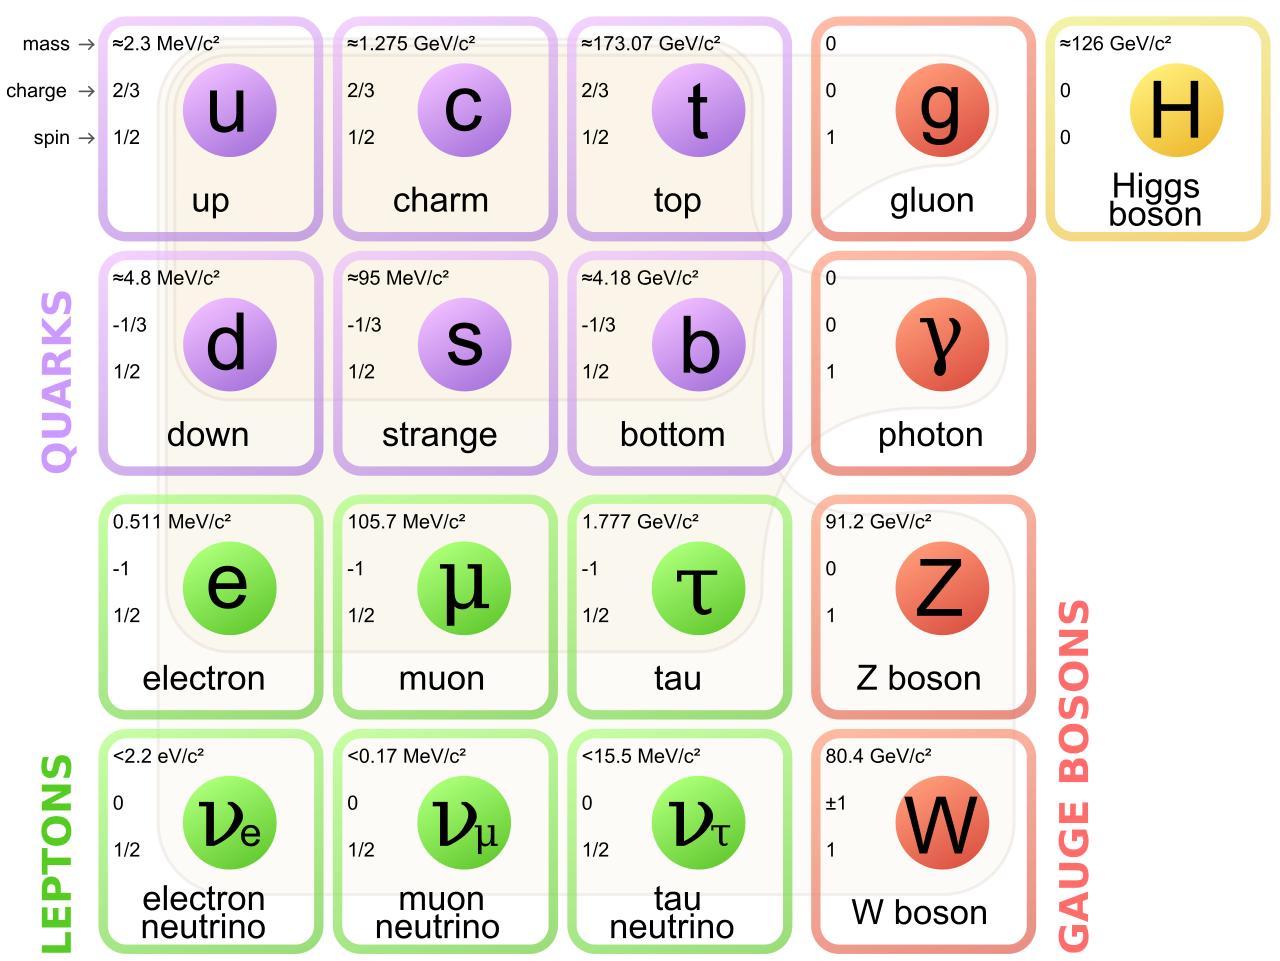
\includegraphics[keepaspectratio,width=0.8\textwidth]{introduction/Standard_Model.png}
\figcaption{The Standard Model of elementary particles and force carriers. This picture is from Wikipedia.}
 \label{standardModel}
\end{figure}

\section{Quantum Chromodynamics}
Quantum Chromodynamics (QCD) is a renormalized non-abelian gauge theory based on the $SU(3)_{C}$ group~\cite{QCDtheory} to describe strong interactions between quarks and gluons. The subscript $C$ denotes the quantum number - color, which is an exact symmetry. Quarks are color triplets while hadrons are assumed to be color singlets in QCD. The invariant QCD Lagrangian requires gauge (gluon) self-interactions due to the non-abelian character of the $SU(3)_{C}$ group. There are eight different gluons, and the gluon exchange can change the color of a quark but not its flavor. QCD has two seemingly-contradictory properties: 1) Asymptotic freedom; 2) Confinement.

\subsection{Asymptotic Freedom and Confinement}
Experimentally, no single quark has ever been isolated. Only the color-neutral quark bound states - hadrons ($q\bar{q}$, $qqq$ or $\bar{q}\bar{q}\bar{q}$) can be observed. This suggests the interaction between quarks and gluons must be strong on large distance scale. However, in the deep inelastic scattering experiments. It was found that with large momentum transfer, the quarks inside the hadron behaved as if they were almost free~\cite{DISasymptotic}. According to the behaviors of short and long distance, the static QCD potential can be described as:
\begin{equation} 
V_{s} = -\frac{4}{3} \times \frac{\alpha_{s}}{r} + k \times r 
\label{QCDpotential}
\end{equation}
where the first term dominating at small distance is similar to the Coulomb potential between two charges in QED, while the second term is linked to the confinement of quarks and gluons inside hadrons.  

The effect coupling constant depends on the renormalization scale, which can be written as: 
\begin{equation} 
\alpha_{s}(\mu) = \frac{g^{2}_{s}(\mu)}{4\pi} \approx \frac{4\pi}{\beta_{0}ln(\mu^{2}/\Lambda^{2}_{QCD})} 
\label{runningConst}
\end{equation}
where $\beta_{0} = (11 - \frac{2}{3}n_{f})$ is a constant, depending on the number of active quark flavors at the energy scale $\mu$ and $\Lambda_{QCD}$ is a constant QCD scale parameter determined experimentally ($\Lambda_{QCD}\approx$ 250 MeV/$c$). Figure~\ref{runningConstant} shows the experimental measurements of $\alpha_{s}$ as a function of Q (momentum transfer)~\cite{runningExp}.

\begin{figure}[htbp]
\centering
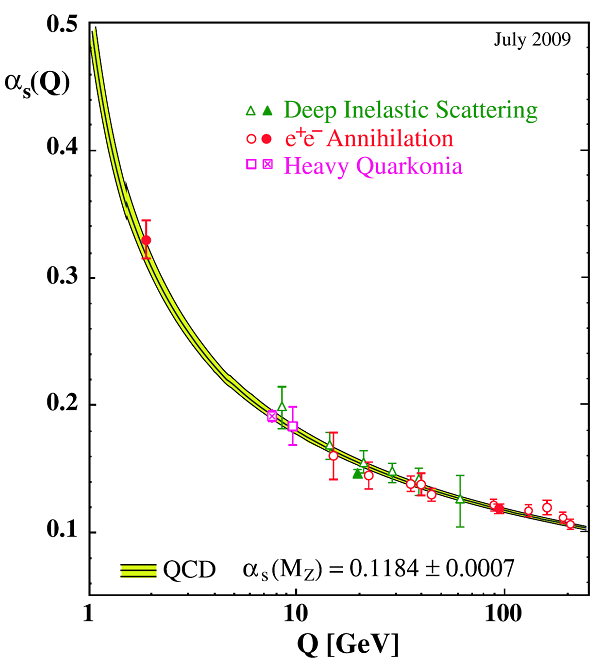
\includegraphics[keepaspectratio,width=0.7\textwidth]{introduction/running_constant.png}
\figcaption{Experimentally measured $\alpha_{s}$ as function of the respective
energy scale Q~\cite{runningExp}.}
 \label{runningConstant}
\end{figure}

With larger $Q^{2}$ (probing small length scales), the $\alpha_{s}$ becomes smaller. The small $\alpha_{s}$ suggests that the quarks and gluons move freely. When $\alpha_{s}\ll$ 1 (high momentum transfer or short distance approach), methods of perturbative QCD (pQCD) are applied to predict the cross sections and distributions of physical processes implying quarks and gluons in the initial, intermediate or final state. On the contrary, with smaller $Q^{2}$ or larger distance ($\alpha_{s}\rightarrow$ 1), the attractive force and gluon binding potential between quarks become larger. When quarks separate, the gluon field form narrow tubes (or strings) of color charge to bring the quarks together. When two quarks have large enough energies and become separated, at some point the gluon field is more energetically favorable to create a new quark and anti-quark pair out of the vacuum than to allow the quarks to separate further. As a result, a new hadron is created instead of seeing free quarks. The QCD coupling constant $\alpha_{s}$ approaches unity quickly as momentum transfer decreases in low-momentum transfer processes. In this case, the high order processes will have large contributions and can not be neglected, thus the pQCD is not valid any more. Instead, the Lattice QCD or other Non-Perturbative QCD (e.g. AdS/CTF - anti-de-Sitter space/conformal field theory) is used to calculate strong interaction processes.

\subsection{Quark Gluon Plasma and Phase Transition}
Quark Matter is mostly observed as quark bound state in normal condition. However, in extreme condition like high temperature or high baryon density, quarks and gluons are proposed to be deconfined from a hadron. A new state of deconfined matter is thus created, so called Quark Gluon Plasma (QGP). In such an environment, long-range interactions are screened by the high density of color charges. Since short-range interactions in QCD are weak, the quarks and gluons (partons) behave as nearly free particles. Lattice QCD calculations show that significant change of $\varepsilon/T^{4}$ ($\varepsilon$ - energy density, $T$ - temperature, this quantity is proportional to the number of degrees of freedom) occurs at the critical temperature ($T_{c}\sim$ 150-180 MeV) as shown in Fig.~\ref{lQCD_PT}~\cite{LQCDPhaseTransistion}, indicating a phase transition. The saturated values are far away from their corresponding Stefan-Boltzmann (ideal gas) expectation. This indicates there are still sizable strong interactions in QGP although the quarks and gluons are deconfined. In other words, the QGP does not behave as a quasi-ideal state of free quarks and gluons, but as an almost perfect dense fluid. There are plenty of evidences (collective flow, jet quenching, quarkonia suppression etc.) for the existence of this new deconfined matter in RHIC experiments~\cite{STARwp,PHENIXwp,PHOBOSwp,BRAHMSwp}.

\begin{figure}[htbp]
\centering
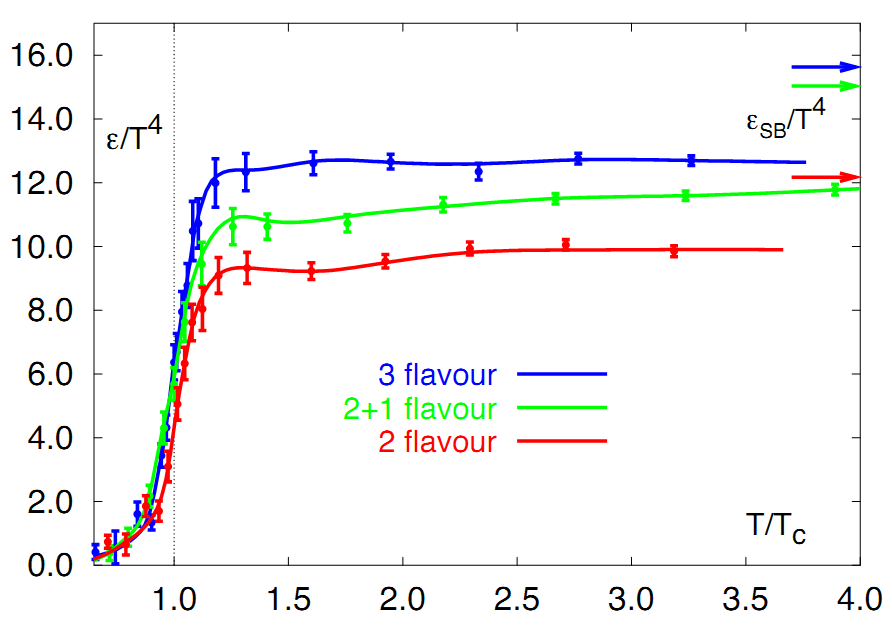
\includegraphics[keepaspectratio,width=0.6\textwidth]{introduction/lQCD_PhaseTransistion.png}
\figcaption{The evolution of $\varepsilon/T^{4}$ as a function of temperature for 3 different flavor scenarios. The arrows indicate the Stefan-Boltzmann limit for each scenario.}
 \label{lQCD_PT}
\end{figure}

\begin{figure}[htbp]
\centering
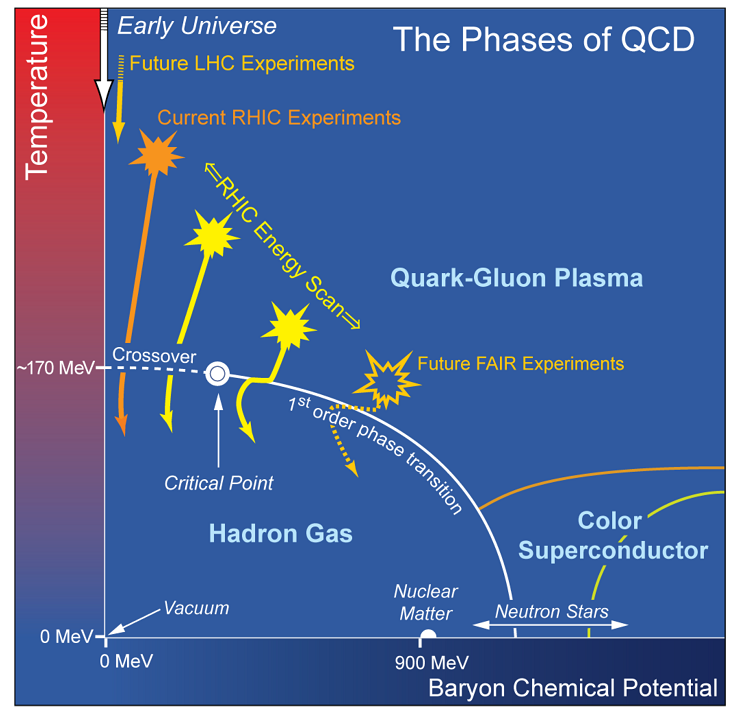
\includegraphics[keepaspectratio,width=0.7\textwidth]{introduction/QCD_phase_diagram.png}
\figcaption{A conjectured QCD phase diagram with boundaries that define various states of QCD matter.}
 \label{QCDpd}
\end{figure}

Figure~\ref{QCDpd} shows a conjectured phase diagram in $T-\mu_{B}$ plane, which describes the phase structure of QCD matter. Lattice QCD calculations predict that the phase transition from hadron gas to the QGP for $T>T_{c}$ at zero baryon chemical potential ($\mu_{B}=$ 0) is expected to be a smooth crossover (white dashed line) instead of a sudden change of energy density. Lattice QCD calculations also predict that there is a first-order phase transition (white solid line) at large $\mu_{B}$, and it is expected to be end in a critical point at finite $\mu_{B}$. The estimation of the location of the critical point~\cite{CriticalPoint} (white dot) is depicted in Fig.~\ref{QCDpd}.

The first RHIC Beam Energy Scan (BES) program was carried out in which data were acquired from Au + Au collisions at $\sqrt{s_{NN}}=$ 62.4, 39, 27, 19.6, 14.5, 11.5, and 7.7 GeV in years 2010, 2011, and 2014~\cite{BESI}. A BES phase \uppercase\expandafter{\romannumeral2} focusing on low collision energies (7.7, 9.1, 11.5, 14.5 and 19.6 GeV) is scheduled to run in years 2019 and 2020~\cite{BESII}. These BES programs can access a broad region of the QCD phase diagram and give us a unique opportunity to search for the QCD critical point and map the first phase boundary.

\subsection{Chiral Symmetry}
The QCD Lagrangian has local $SU(3)_{color}$ gauge symmetry and several global symmetries. For instance,  the $U(1)$ symmetry which entails the baryon number conservation. The QCD Lagrangian has additional symmetries for vanishing quark masses. Compared to momentum transfer of 1 GeV/$c$, the up-, down- and strange-quarks can be treated massless. The Lagrangian is invariant under global vector and axial-vector transformations in $SU(3)$-flavor space
\begin{equation} 
\psi \rightarrow e^{-i\alpha^{i}_{V}\frac{\lambda^{i}}{2}}\psi,  \;\;  \psi \rightarrow e^{-i\alpha^{i}_{A}\frac{\lambda^{i}}{2}\gamma_{5}}\psi
\label{Vec_axiVec_sym}
\end{equation}
When decomposing the quark fields into left and right chirality components, $\psi_{L,R} = \frac{1}{2}(1\mp\gamma_{5})\psi$, the transformations (Eq.~\ref{Vec_axiVec_sym}) translate to 
\begin{equation} 
\psi_{L} \rightarrow e^{-i\alpha^{i}_{L}\frac{\lambda^{i}}{2}}\psi_{L},  \;\;  \psi_{R} \rightarrow \psi_{R}
\label{Left_sym}
\end{equation}
\begin{equation} 
\psi_{R} \rightarrow e^{-i\alpha^{i}_{R}\frac{\lambda^{i}}{2}}\psi_{R},  \;\;  \psi_{L} \rightarrow \psi_{L}
\label{Right_sym}
\end{equation}
which constitutes a global $SU(3)_{L} \times SU(3)_{R}$ chiral symmetry in the limit of vanishing quark masses in flavor space. 

\paragraph{Spontaneous Breaking of Chiral Symmetry}
Symmetry breaking can be distinguished into two types, explicit symmetry breaking and spontaneous symmetry breaking, characterized by whether the equations of motion fail to be invariant or the ground state fails to be invariant. In spontaneous symmetry breaking, the equations of motion of the system are invariant, but the system is not because the ground state is not invariant. We consider a symmetrical upward dome with a though circling the bottom, as shown in Fig.~\ref{MexicanHat}. If a ball is put at the very peak of the dome, the system is symmetrical under center-axial rotation. However, the system is very unstable, the ball will roll down the dome into the trough, a point of the lowest energy, with a small fluctuation on the system. In this scenario, any point in the trough could be the ground state. Obviously, the ground state is not symmetrical, resulting in spontaneous symmetry breaking.

\begin{figure}[htbp]
\centering
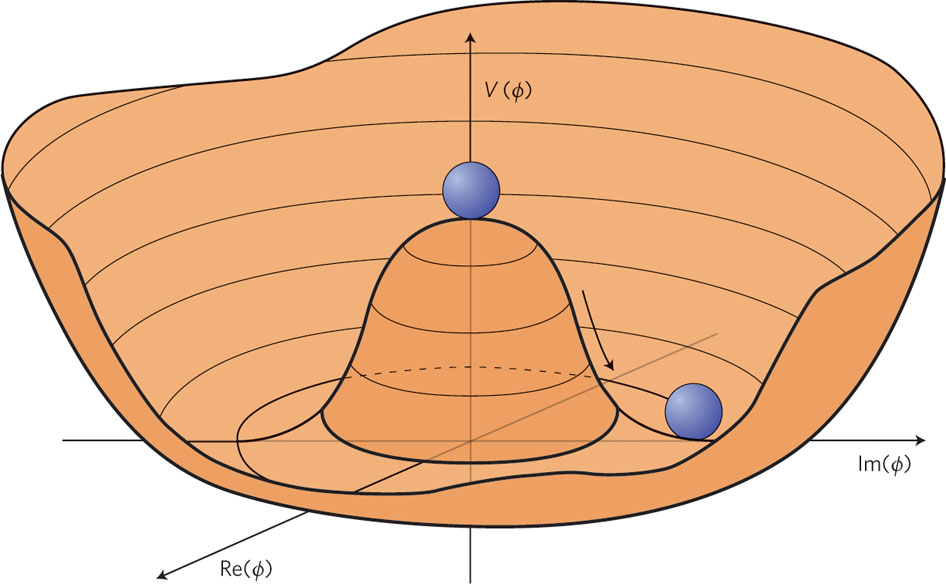
\includegraphics[keepaspectratio,width=0.5\textwidth]{introduction/Mexican_hat.png}
\figcaption{Goldstone's ``Mexican hat'' potential function V versus $\phi$.}
 \label{MexicanHat}
\end{figure}

Chiral symmetry breaking is an example of spontaneous symmetry breaking affecting the chiral symmetry of the strong interactions in particle physics. The vacuum quark condensate can be expressed as the Gell-Mann-Oakes-Renner relation:
\begin{equation} 
m^{2}_{\pi}f^{2}_{\pi} = -2\bar{m}\langle\bar{q}q\rangle
\label{GORrelation}
\end{equation}
where $\bar{m}$ is the average mass of up and down quarks. With $\bar{m}=$ 6 MeV, $m_{\pi}=$ 140 MeV and $f_{\pi}=$ 93.2 MeV, the vacuum condensate is $\langle\bar{q}q\rangle \approx$ (-250 MeV)$^{3}$. A finite quark condensate implies that chiral symmetry is spontaneously broken.  The chiral partner $\rho^{0}$ and $a_{1}(1260)$ have quite different masses ($m_{\rho^{0}}=$ 770 MeV and $m_{a_{1}}=$ 1260 MeV) provides an experimental evidence for spontaneous breaking of chiral symmetry. According to the Goldstone theorem, the spontaneous breaking of chiral symmetry results in the existence of eight massless (very light) Goldstone bosons ($\pi^{\pm}$, $\pi^{0}$, $K^{\pm}$, $K^{0}$, $\bar{K}^{0}$ and $\eta$). 

\paragraph{Restoration of Chiral Symmetry}
In the ultra-relativistic heavy-ion collisions, it is to be expected that the quark and gluon condensates are modified at finite temperature, $T$, and quark chemical potential, $\mu_{q}$. Chiral symmetry restoration can be characterized by the rapid decrease of the quark condensates. Lattice QCD calculations predict a phase transition from hadronic phase to the Quark Gluon Plasma (QGP) phase at high temperature ($T$) and low baryon density or at high baryon density region. The quark condensates are melted in the hot and dense medium, resulting in the restoration of chiral symmetry. The chiral partners will be degenerate when the chiral symmetry restores, which leads to massive medium modifications of hadronic spectral functions as the phase transition approaches. The $\rho$ meson is a unique particle to study the chiral properties of the hot and dense medium, since its life time is much short ($\sim$1.3 fm/$c$) than that of medium ($\sim$10 fm/$c$) created in heavy-ion collisions. Thus $\rho$ meson spectral is very sensitive to the hadronic medium and expected to be significant modified during the system evolution.

\section{Dilepton Production in Heavy-ion Collisions}
\label{dilepton:physics}
Heavy-ion collisions have been pursued for more than several decades for searching and studying the quantum chromodynamics (QCD) matter in the laboratory. Several heavy-ion colliders have been conducted, such as Alternating Gradient Synchrotron (AGS) at BNL, Super Proton Synchrotron (SPS) at CERN, Relativistic Heavy Ion Collider (RHIC) at BNL and Large Hadron Collider (LHC) at CERN. Since year 2000, the RHIC has been operating and providing collisions to its two large experiments STAR and PHENIX, and its two small experiments PHOBOS (decommissioned in 2005) and BRAHMS (decommissioned in 2006). All of these four experiments reported the results from first three years in 2005, and argued that a strongly coupled quark gluon plasma (sQGP) had been established in high-energy heavy-ion collisions~\cite{STARwp,PHENIXwp,PHOBOSwp,BRAHMSwp}. There have been two runs (years 2010 and 2011) at the LHC with Pb + Pb collisions at $\sqrt{s_{NN}}$ = 2.76 TeV, fourteen times higher than RHIC top energy, resulting in hotter, larger size and longer lifetime fire ball. Many of the RHIC findings of the properties of the QGP medium are confirmed by the LHC experiments.

As electromagnetic probes, dileptons play a crucial role in probing hot and dense nuclear matter created in the relativistic heavy-ion collisions. Dileptons are produced in the whole evolution of the created matter and escape with minimum interaction with the strongly interacting medium. Thus, they provide information about the various stages of the system during the evolution. According to different physics interests, the dilepton invariant mass spectrum is typically divided into three ranges: the Low Mass Region (LMR, $M_{ll}<M_{\phi}$), the Intermediate Mass Region (IMR, $M_{\phi}<M_{ll}<M_{J/\psi}$) and the High Mass Region (HMR, $M_{ll}>M_{J/\psi}$), to probe the properties of the created matter throughout its entire evolution.

In the HMR, the dileptons are produced by the initial hard pertubative QCD processes. For instance, the Drell-Yan production ($q\bar{q} \rightarrow \gamma^{*}/Z \rightarrow l^{+}l^{-}$), semi-leptonic decays of correlated heavy quark pairs ($b\bar{b} \rightarrow l^{+}l^{-}$) and heavy quarkonia (J/$\psi$, $\varUpsilon$ etc.). Thus dileptons in the HMR are used to probe the initial stage of the collision~\cite{InitialDilepton}. For instance, the J/$\psi$, $\varUpsilon$ and their excited states are used to study the color screening features of the QGP~\cite{JpsiDeconfinement}.

In the IMR, the dileptons are expected to be directly related to the thermal radiation of the QGP. Theoretical calculations indicate that the QGP thermal dilepton production will become a dominate source in the IMR at top RHIC energy. Thermal dileptons with higher masses originate from earlier stages~\cite{broaden1}. The measurement of the thermal dilepton yields can be used to determine the initial temperature of the QGP medium. However, to measure the dielepton from QGP thermal radiation, the significant contributions from the semi-leptonic decays of correlated open heavy flavor should be measured (e.g.  $c + \overline{c} \rightarrow e + \mu, b \rightarrow e(\mu) + c \rightarrow e + \mu$ ) and subtracted experimentally first.
 
 In the LMR, the dilepton production is dominated by in-medium decay of vector mesons ($\rho$, $\omega$, $\phi$, etc.) and also contributed by long-lived hadron decays ($\pi^{0}$, $\eta$, $\eta^{\prime}$, etc.). Theoretical calculations suggest that the vector meson spectral functions will undergo modifications in a hot and dense hadronic medium, which are considered as a link to chiral symmetry restoration~\cite{broaden0,broaden1,broaden2}. In the vacuum, the chiral symmetry is spontaneously broken, resulting in mass differences between chiral partners (e.g. $\rho$ and $a_{1}$(1260)). In the hot and dense medium, the chiral symmetry is expected to restore, resulting in the degeneration of $\rho$ and $a_{1}(1260)$. However, it is impossible to measure a spectral function for the $a_{1}$(1260) in the heavy-ion collisions. Instead, efforts are devoted to study the modification of vector meson spectral function, and then models are employed to connect the modification function to the chiral symmetry restoration. Two scenarios have been used to describe the in-medium $\rho$ spectral function when chiral symmetry is restored: a dropping mass $\rho$~\cite{dropmass} and a broadened $\rho$~\cite{broaden2}. The dilepton measurements in LMR will map the vector meson production mechanisms, and thus the chiral properties of the medium in heavy-ion collisions. The contributions from long-lived hadron decays can be simulated based on the measured or predicted $p_{T}$ spectra and yields of the involved parent particles, so called hadronic cocktails.

\section{Previous Dilepton Measurements}
For the past decades, lots of dilepton measurements have been carried out in heavy-ion collisions from low to ultrarelativistic energies. For instance, DLS at Bevalac~\cite{DLS:dielectron0,DLS:dielectron1}; HADES at SIS18~\cite{HADES:dielectron0,HADES:dielectron1,HADES:dielectron2,HADES:dielectron3}; HELIOS/3~\cite{HELIOS:dimuon}, NA38/50~\cite{NA38:dimuon,NA50:dimuon}, CERES/NA45 and NA60 at SPS~\cite{CERES:dielectron0,CERES:dielectron1,CERES:dielectron2,CERES:dielectron3,NA60:dimuon0,NA60:dimuon1,NA60:dimuon2}; PHENIX and STAR at RHIC~\cite{PHENIX:dielectron0,PHENIX:dielectron1,STAR:dielectron0,STAR:dielectron1:PRL,STAR:dielectron1,STAR:dielectron2}; ALICE at LHC~\cite{ALICE:dielectron}. In this section, only the results of relevant experiments are briefly discussed. 

\subsection{HADES Experiment}

\begin{figure}[htbp]
\begin{minipage}[htbp]{0.42\linewidth}
\centering
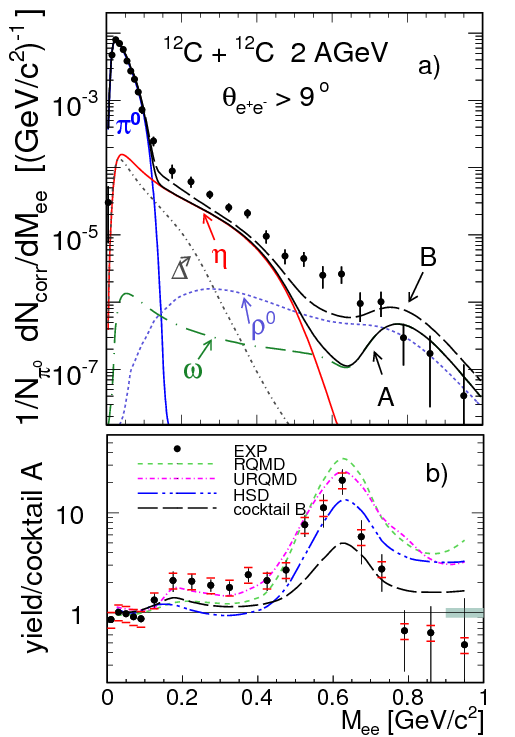
\includegraphics[width=1.0\textwidth]{introduction/HADES_CC_2GeV.png}
\caption{(Top) Dielectron spectrum within HADES acceptance (black dots) together with hadronic cocktail simulations without (Cocktail A, black solid line) and with (Cocktail B, black dashed line) $\Delta(1232)$ and $\rho$ contributions. (Bottom) The ratios of data over cocktail A and cocktail B over cocktail A, together with various model calculations. \label{hades_cc2gev}}
\end{minipage}
\hfill
\begin{minipage}[htbp]{0.56\linewidth}
\centering
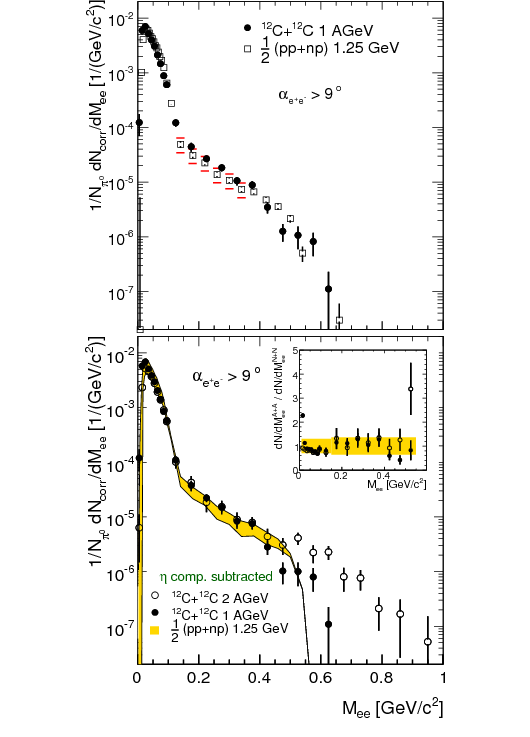
\includegraphics[width=1.0\textwidth]{introduction/HADES_NN_scale.png} 
\caption{(Top) Comparison of the dielectron invariant mass spectrum in $^{12}$C + $^{12}$C collisions at 1 GeV/$u$ (black dots) with an isospin-averaged reference from $p$ + $p$ and $n$ + $p$ collisions (open squares). (Bottom) Comparison of the reference spectrum from elementary collisions with spectra for $^{12}$C + $^{12}$C at 1 (black dots) and 2 GeV/$u$ (open circles). The contribution from $\eta$ Dalitz decay have been subtracted.\label{hades_nnscale}}
\end{minipage}
\end{figure}

\begin{figure}[htbp]
\centering
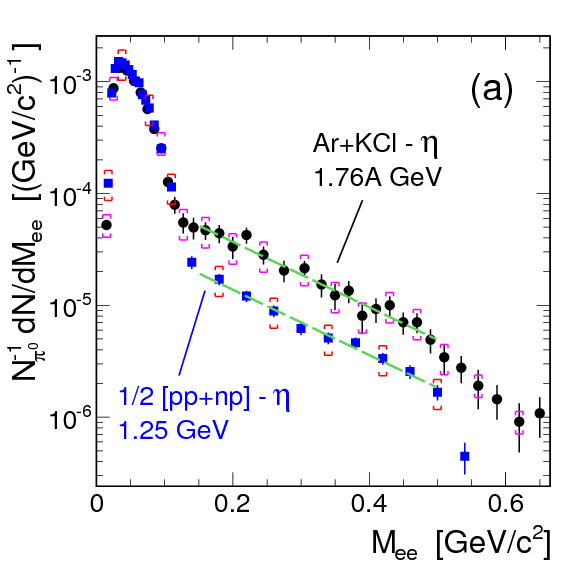
\includegraphics[width=0.48\textwidth]{introduction/HADES_ArKl_0.png}
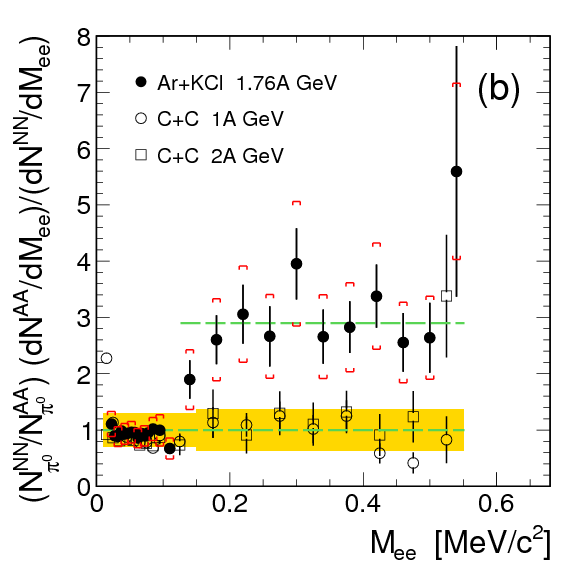
\includegraphics[width=0.48\textwidth]{introduction/HADES_ArKl_1.png}
\figcaption{(Left)  Comparison of the dielectron invariant mass spectrum (subtracted $\eta$ contribution) in Ar + KCl collisions (black dots) with an isospin-averaged reference from $p$ + $p$ and $n$ + $p$ collisions (blue solid squares). (Right) Ratios of $\eta$ contribution subtracted dielectron invariant mass spectra for different collision systems over the reference from $p$ + $p$ and $n$ + $p$ collisions.}
\label{hades_arkcl}
\end{figure}
  
The High-Acceptance DiElectron Spectrometer (HADES) is a fixed target experiment, operated at GSI, with proton and heavy-ion beams being provided by the synchrotron SIS18. HADES reported the dielectron spectra produced in $^{12}$C + $^{12}$C collisions at incident energies of 1 GeV and 2 GeV per nucleon~\cite{HADES:dielectron0,HADES:dielectron1}, and the efficiency-corrected dielectron spectrum within HADES accepctance of 2 A GeV is shown in Fig.~\ref{hades_cc2gev}. The measured dielectron continuum is consistent with the hadronic sources (cocktail) in $\pi^{0}$ region ($M_{ee}<$ 0.15 GeV/$c^{2}$), but a strong excess with respect to cocktail is observed in $M_{ee}>$ 0.15 GeV/$c^{2}$ at both energies. Various transport model calculations are employed, but no one can fully describe the excess. Moreover, the measurements of the excess yields (0.15 $<M_{ee}<$ 0.5 GeV/$c^{2}$) between 1 and 2 A GeV demonstrate that the excess scaled with bombarding energy like pion production, rather than like the production of the much heavier η meson. 
 
HADES also performed the dielectron measurements in elementary $p$ + $p$ and $d$ + $p$ (selecting quasi-free $n$ + $p$ reactions) at incident energy of 1.25 GeV per nucleon~\cite{HADES:dielectron2}. The yield of electron pairs with $M_{ee}>$ 0.15 GeV/$c^{2}$ in quasi-free $n$ + $p$ collisions is about an order of magnitude larger than that in $p$ + $p$ collisions (isospin dependence). Moreover, the excess spectra observed in $^{12}$C + $^{12}$C collisions in 0.15 $<M_{ee}<$ 0.5 GeV/$c^{2}$ at 1 and 2 GeV/$u$ can be described by a superposition of elementary $p$ + $p$ and $n$ + $p$ collisions, as shown in Fig.~\ref{hades_nnscale}, leaving little room for additional electron pair sources in such light collision systems. More recently, the measurements of the dielectron production in Ar + KCl collisions at incident energy of 1.76 GeV per nucleon, observe a significant excess (up to a factor of three) with respect to the $NN$ reference in 0.15 $<M_{ee}<$ 0.5 GeV/$c^{2}$, as shown in Fig.~\ref{hades_arkcl}. This proves that a qualitative change happens in the nature of the excess yield when going to the heavier system, requiring contributions from other sources (e.g. in-medium modifications of the involved hadrons).

\subsection{CERES/NA45 Experiment}
CERES/NA45 is a fixed target experiment dedicated to the measurement of dielectron in the low-mass range from 50 MeV/$c^{2}$ to $\sim$1.5 GeV/$c^{2}$ at the CERN Super Proton Synchrotron (SPS). Particle identification and directional tracking are based on two azimuthally symmetric RICH (ring imaging Cherenkov) detectors, and a detailed description of the CERES/NA45 experiment can be found in~\cite{CERES:experiment}.
 
CERES reported on the measurements of low-mass dielectron spectra in 450 GeV $p$-Be, $p$-Au and 200 A GeV S-Au collisions~\cite{CERES:dielectron0,CERES:dielectron1}. The results are shown in Fig.~\ref{ceres_pASAu}. The measurements of $p$-A can be reproduced within statistical and systematic errors by the hadronic cocktail simulations. However, a significant enhancement with respect to the hadronic cocktail is observed  in $M_{ee}>$ 0.25 GeV/$c^{2}$ in 200 A GeV S-Au collisions. Further dielectron measurements performed in Pb-Au at 40 and 158 A GeV by CERES~\cite{CERES:dielectron2,CERES:dielectron3}, confirm this low-mass region enhancement, as shown in Fig.~\ref{ceres_PbAu}. The $p_{T}^{ee}$ and centrality dependence of the excess spectra have also been studied in Pb-Au collisions at 158 A GeV. The results show the enhancement mostly occurs in low $p_{T}$ region and has a strong centrality dependence. 

\begin{figure}[htbp]
\centering
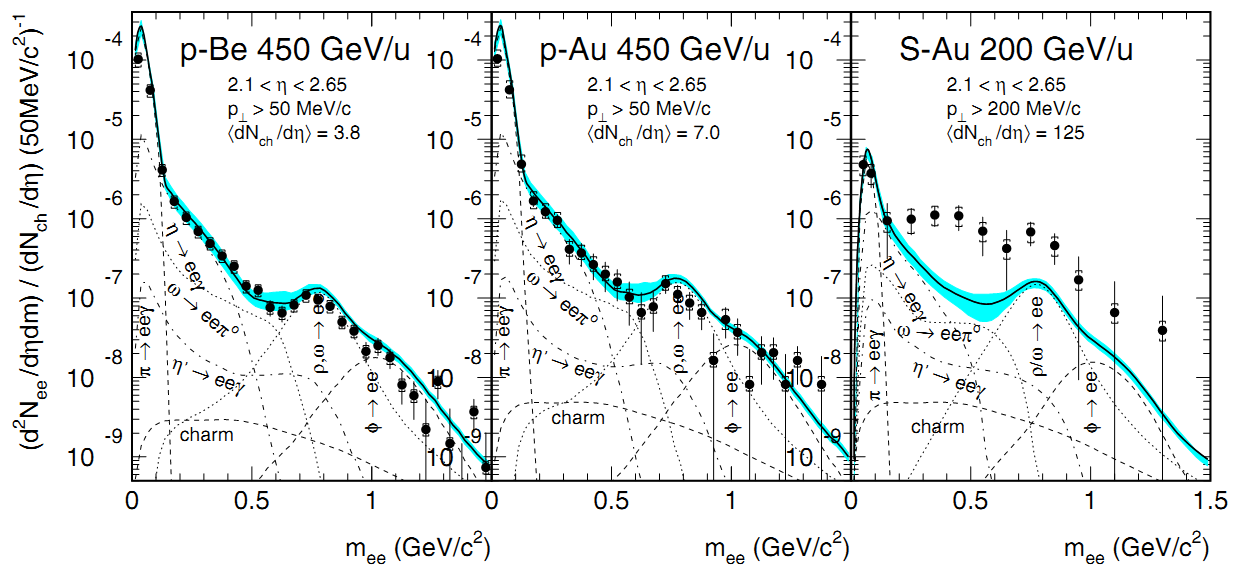
\includegraphics[keepaspectratio,width=1.0\textwidth]{introduction/CERES_pA_SAu.png}
\figcaption{Inclusive dielectron invariant mass spectra (black dots) together with corresponding hadronic cocktails (black solid lines) within CERES acceptance in 450 GeV $p$-Be (Left), $p$-Au (Middle) and 200 A GeV S-Au (Right) collisions.}
 \label{ceres_pASAu}
\end{figure}

\begin{figure}[htbp]
\centering
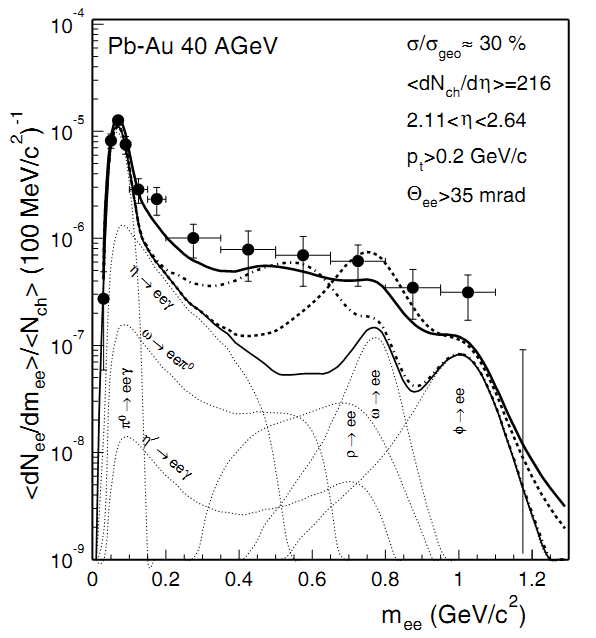
\includegraphics[width=0.468\textwidth]{introduction/CERES_PbAu_40GeV.png}
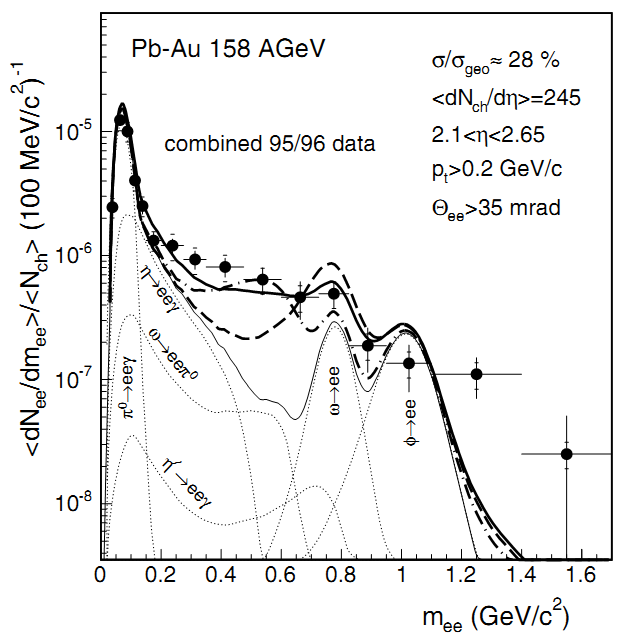
\includegraphics[width=0.48\textwidth]{introduction/CERES_PbAu_158GeV.png}
\figcaption{Comparison of the inclusive mass spectra (black dots) to (i) hadronic cocktails without ρ decay (thin solid line), (ii) model calculations with a vacuum ρ spectral function (thick
dashed line), (iii) with dropping in-medium ρ mass (thick dashed-dotted line), (iv) with a medium-modified ρ spectral function (thick solid line) in Pb-Au collisions at 40 A GeV (Left) and 158 A GeV (Right).}
\label{ceres_PbAu}
\end{figure}

At top SPS energy, the primary candidate for ``thermal radiation'' from the hadronic phase of the fireball is pion annihilation ($\pi^{+}\pi^{-} \rightleftharpoons \rho \rightarrow e^{+}e^{-}$). However, various theoretical models incorporating pion annihilation using vacuum $\rho$ spectral function, fail to describe the data. Thus theoretical calculations incorporating the in-medium modification of $\rho$ meson attempt to reproduce the CERES low-mass region enhancement. Two scenarios are used to describe the in-medium $\rho$ spectrum function: a dropping-mass $\rho$~\cite{dropmass} and a broadened $\rho$~\cite{broaden0}. However, these two scenarios can not be discriminated due to the limited CERES data quality.

\subsection{NA60 Experiment}
NA60 is a fixed target experiment, aiming to study the phase transition from confined hadronic matter to deconfined partonic matter, operated at CERN SPS. NA60 inherits muon spectrometer and zero degree calorimeter previously used in NA38/50~\cite{NA60:dimuon2}. More importantly, a novel radiation-hard silicon pixel vertex tracker with high granularity and high readout speed, placed inside a 2.5 T dipole magnet, is installed the downstream of the targets. Combining the vertex tracker and muon spectrometer, the dimuon mass resolution is significantly improved and the combinatorial background due to $\pi/K$ decays is significantly reduced. Furthermore, the muon offset with respect to the primary interaction vertex can be measured which is essential to distinguish the prompt (Drell-Yan and thermal radiation etc.) and off-vertex (correlated open charm decays) dimuon pairs. The schematic view of the NA60 experiment is shown in Fig.~\ref{NA60experiment}.

\begin{figure}[htbp]
\centering
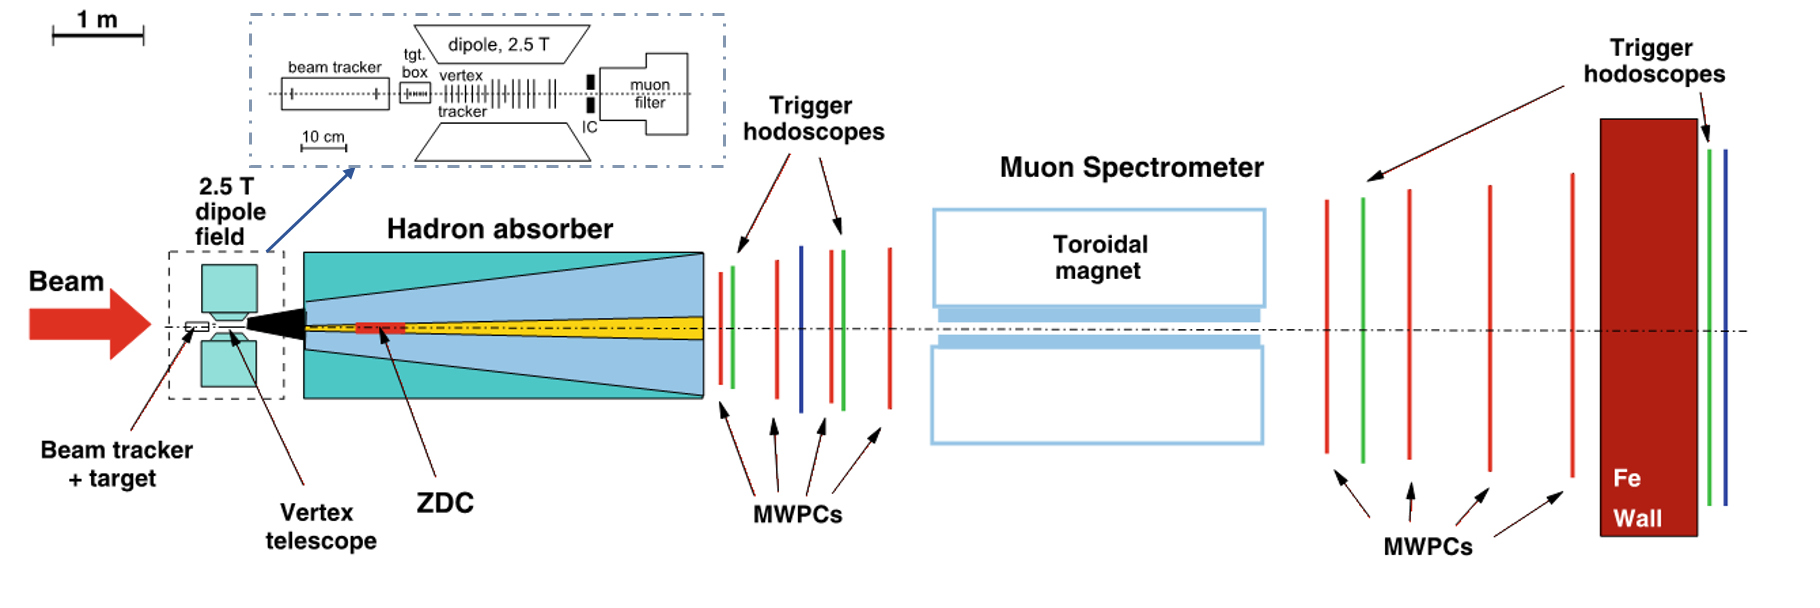
\includegraphics[keepaspectratio,width=1.0\textwidth]{introduction/NA60_experiment.png}
\figcaption{Schematic view of the NA60 experiment.}
 \label{NA60experiment}
\end{figure}

A systematic study of the low mass dimuon spectrum ($M_{\mu\mu}<$ 1.4 GeV/$c^{2}$) has been performed by NA60 using the high precision data in In + In collisions at 158 A GeV. In the most peripheral collisions, the dimuon spectrum can be reproduced by the hadronic cocktail (including the vacuum $\rho$)~\cite{NA60:dimuon0}. However, the dimuon spectrum in the central collisions can not described by the hadronic cocktail any more. A significant enhancement with respect to the hadronic cocktail (excluding $\rho$) is observed, and the excess yield has a strong centrality dependence~\cite{NA60:dimuon3}. The left panel of Fig.~\ref{NA60_LMR_excess} shows the centrality-integrated dimuon mass spectra within NA60 acceptance before (red dots) and after (black triangles) subtraction of the hadronic cocktail (excluding $\rho$), and the right panel shows the excess spectrum in semi-central collisions together with various theoretical model calculations. The theoretical model calculation based on vacuum $\rho$ is clearly ruled out, and the dropping mass scenario which reasonably described the CERES data is also ruled out by the much precise NA60 data. The theoretical model calculation incorporating a broadened $\rho$ spectral function, describes the data reasonably well.

\begin{figure}[htbp]
\centering
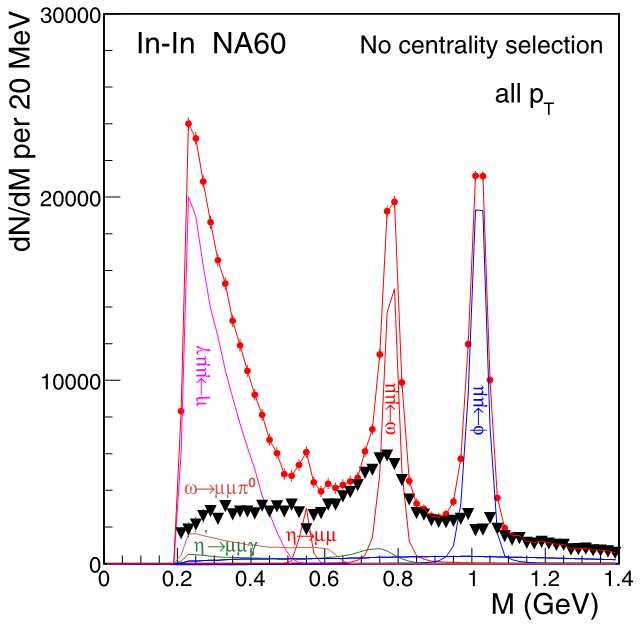
\includegraphics[keepaspectratio,width=0.49\textwidth]{introduction/NA60_LMR_Spec0.png}
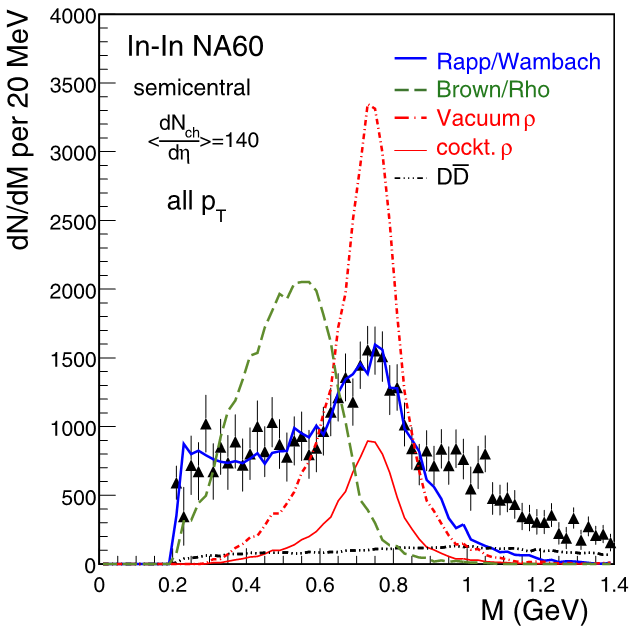
\includegraphics[keepaspectratio,width=0.49\textwidth]{introduction/NA60_LMR_Spec1.png}
\figcaption{(Left) The dimuon spectra within NA60 acceptance before (red dots) and after (black triangles) subtracting the hadronic cocktail (excluding $\rho$). (Right) Excess spectrum within NA60 acceptance in semi-central collisions together with various theoretical model calculations.}
 \label{NA60_LMR_excess}
\end{figure}

For the IMR, thanks to the high position resolution vertex tracker ($\sigma_{x}<$ 10 $\mu$m, $\sigma_{y}<$15 $\mu$m)~\cite{NA60:dimuon2}, the dimuon weighted offset can be measured. The left panel of Fig.~\ref{NA60_IMRdimuon}~\cite{NA60:dimuon2,NA60:dimuon5} shows the dimuon weighted offset distribution for the inclusive dimuon signals in 1.16 $<M_{\mu\mu}<$ 2.56 GeV/$c^{2}$, which is fitted by that of prompt dimuons and open charm decays. The charm cross section is determined by scaling down the NA50 measurements in p-A collisions~\cite{NA50:dimuon}. The fit result shows that the IMR excess is not from the enhancement of open charm decays. After detector acceptance correction, the excess mass spectrum is obtained by subtracting of the open charm and Drell-Yan contributions. The IMR excess mass spectrum drops off much more steeply with mass than that of Drell-Yan pairs while the shape of excess mass spectrum is pretty similar with that of open charms, as shown in the right panel of Fig.~\ref{NA60_IMRdimuon}. Moreover, the excess $p_{T}$ spectra of the three sub mass regions in IMR and ratio of excess over Drell-Yan as a function of $p_{T}^{\mu\mu}$ are also measured, which show the excess in IMR is also not from the enhancement of Drell-Yan process. Strikingly, after removal of the contributions of the correlated open charm (LMR and IMR) and Drell-Yan (only for IMR), the inverse slope parameters ($T_{eff}$) of acceptance-corrected excess $m_{T}$-spectra as a function of  dimuon invariant mass is also measured, as shown in Fig.~\ref{NA60_Teff}. The $T_{eff}$ shows a monotonically rise with mass from dimuon threshold to the nominal pole of $\rho$ meson, and then following a sudden decline by about 50 MeV down to the IMR values. The initial rise is consistent with the expectation for radial flow of an in-medium hadron-like source decaying into dimuon pairs. The sudden decline suggests a transition to a different source, for instance, partonic source argued by NA60 which flow has not yet built up~\cite{NA60:dimuon1,NA60:dimuon2,NA60:dimuon3}.

\begin{figure}[htbp]
\centering
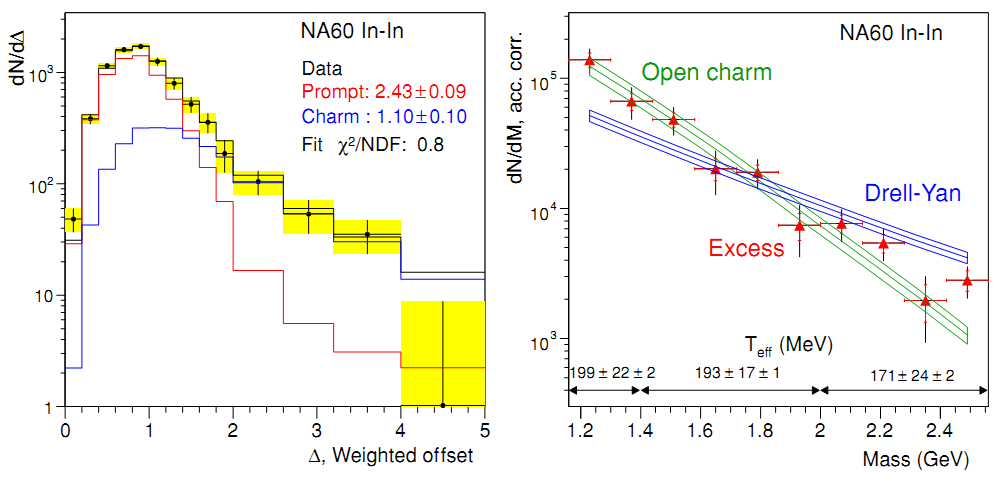
\includegraphics[keepaspectratio,width=1.0\textwidth]{introduction/NA60_dimuon_IMR.png}
\figcaption{(Left) The dimuon weighted offset distribution for the inclusive dimuon signals in 1.16 $<M_{\mu\mu}<$ 2.56 GeV/$c^{2}$ and the comparison with the sum of prompt dimuons and open charm decays. (Right) The detector acceptance corrected mass spectra of all three contributions (excess, Drell-Yan, open charm decays).}
 \label{NA60_IMRdimuon}
\end{figure}

\begin{figure}[htbp]
\centering
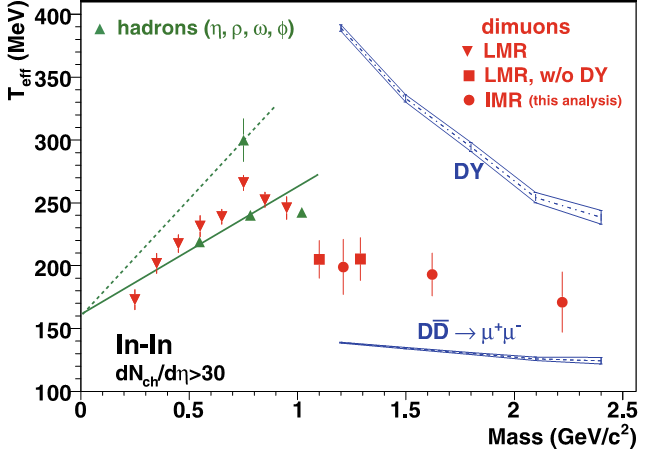
\includegraphics[keepaspectratio,width=0.6\textwidth]{introduction/NA60_InverseSlope.png}
\figcaption{Inverse slope parameter $T_{eff}$ of excess $m_{T}$-spectra as a function of dimuon invariant mass.}
 \label{NA60_Teff}
\end{figure}

\subsection{PHENIX Experiment}
The Pioneering High Energy Nuclear Interaction eXperiment (PHENIX) is one of two large experiments at RHIC. PHENIX is designed specifically to measure direct probes of the collisions such as electrons, muons, and photons.  A detailed description of the detector can be found in~\cite{PHENIX:overview, PHENIX:HBD}.

PHENIX reported the dielectron measurement within PHENIX acceptance in $p$ + $p$ collisions at $\sqrt{s_{NN}}$ = 200 GeV~\cite{PHENIX:dielectron0}, as shown in Fig.~\ref{PHENIX_pp200Spec}, showing that the data can be reproduced by the electromagnetic decays of neutral mesons. The latest dielecton measurements within PHENIX acceptance in Au + Au collisions at $\sqrt{s_{NN}}$ = 200 GeV~\cite{PHENIX:dielectron0}, as shown in Fig.~\ref{PHENIX_AuAu200Spec}, shows that a significant enhancement with respect to the hadronic cocktail can be observed in the LMR. The enhancement factor in 0.30 $<M_{ee}<$ 0.76 GeV/$c^{2}$ is 2.3 $\pm$ 0.4(stat.) $\pm$ 0.4(sys.) $\pm$ 0.2(model) or 1.7 $\pm$ 0.3(stat.) $\pm$ 0.3(sys.) $\pm$ 0.2(model) when the open heavy flavor contribution is  calculated with PYTHIA or MC@NLO, respectively. The new enhancement factor is consistent with that reported by STAR within uncertainty~\cite{STAR:dielectron1}.

\begin{figure}[htbp]
\begin{minipage}[htbp]{0.49\linewidth}
\centering
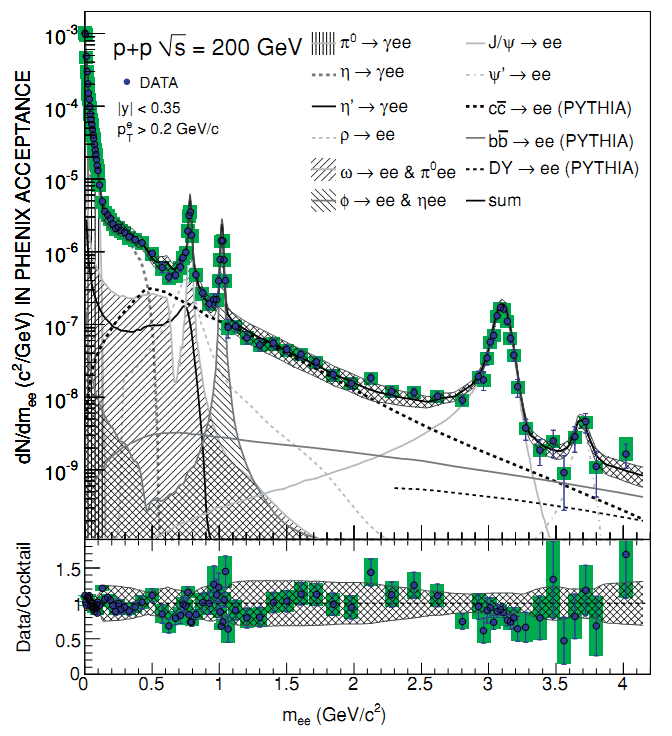
\includegraphics[width=1.0\textwidth]{introduction/PHENIX_pp200.png}
\caption{(Top) Inclusive dielectron invariant mass spectrum together with hadronic cocktail within PHENIX acceptance in $p$ + $p$ collisions at $\sqrt{s_{NN}}$ = 200 GeV. (Bottom) The ratio of data over cocktail as a function of invariant mass. \label{PHENIX_pp200Spec}}
\end{minipage}
\hfill
\begin{minipage}[htbp]{0.49\linewidth}
\centering
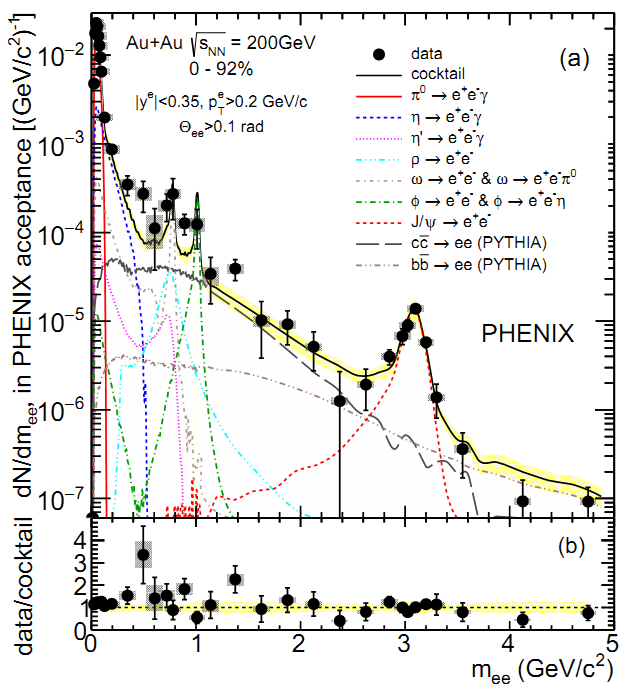
\includegraphics[width=1.0\textwidth]{introduction/PHENIX_AuAu200.png} 
\caption{(Top) Inclusive dielectron invariant mass spectrum together with hadronic cocktail within PHENIX acceptance in Au + Au minimum-bias collisions at $\sqrt{s_{NN}}$ = 200 GeV. (Bottom) The ratio of data over cocktail as a function of invariant mass.\label{PHENIX_AuAu200Spec}}
\end{minipage}
\end{figure}

A theoretical model from Rapp~\cite{broaden0,broaden1,broaden4} incorporating a broadened $\rho$ spectral function and QGP thermal radiation is employed to compare to the PHENIX data, as shown in Fig.~\ref{PHENIX_LMRexcessSpec}. The data can be reasonably described by the model calculation. The integrated excess yield (excess spectrum: data - cocktail) in 0.30 $<M_{ee}<$ 0.76 GeV/$c^{2}$ normalized by number of participants ($N_{part}$) as a function of $N_{part}$ is also measured and shown in Fig.~\ref{PHENIX_LMRexcessYield}. The integrated yield increases faster than $N_{part}$ scaling and is consistent with a expected power-law scaling.

\begin{figure}[htbp]
\begin{minipage}[htbp]{0.49\linewidth}
\centering
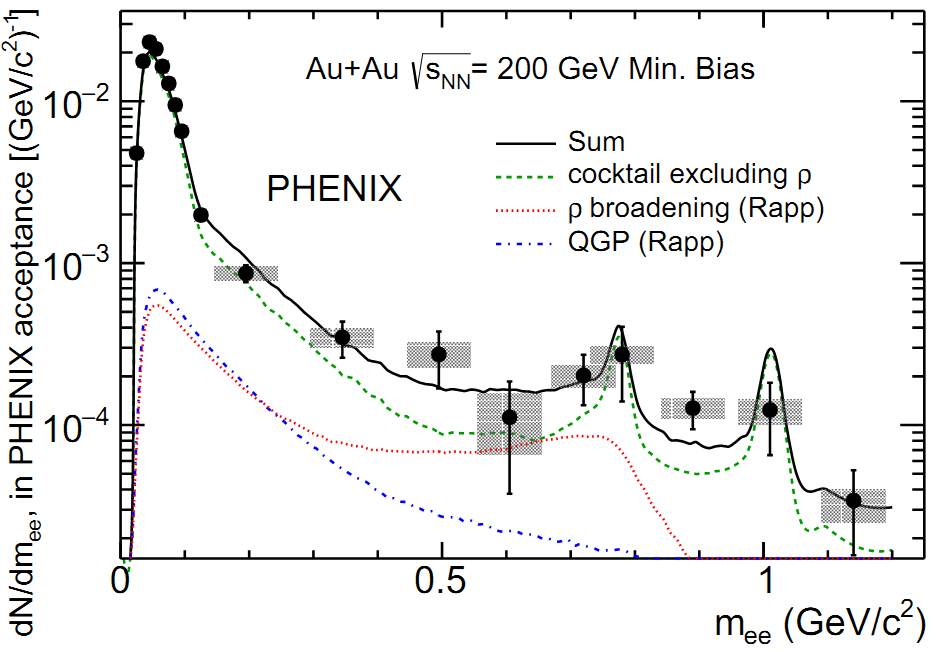
\includegraphics[width=1.0\textwidth]{introduction/PHENIX_LMexcess_Theo.png}
\caption{The minimum-bias invariant mass spectrum together with the model calculations of Rapp. \label{PHENIX_LMRexcessSpec}}
\end{minipage}
\hfill
\begin{minipage}[htbp]{0.49\linewidth}
\centering
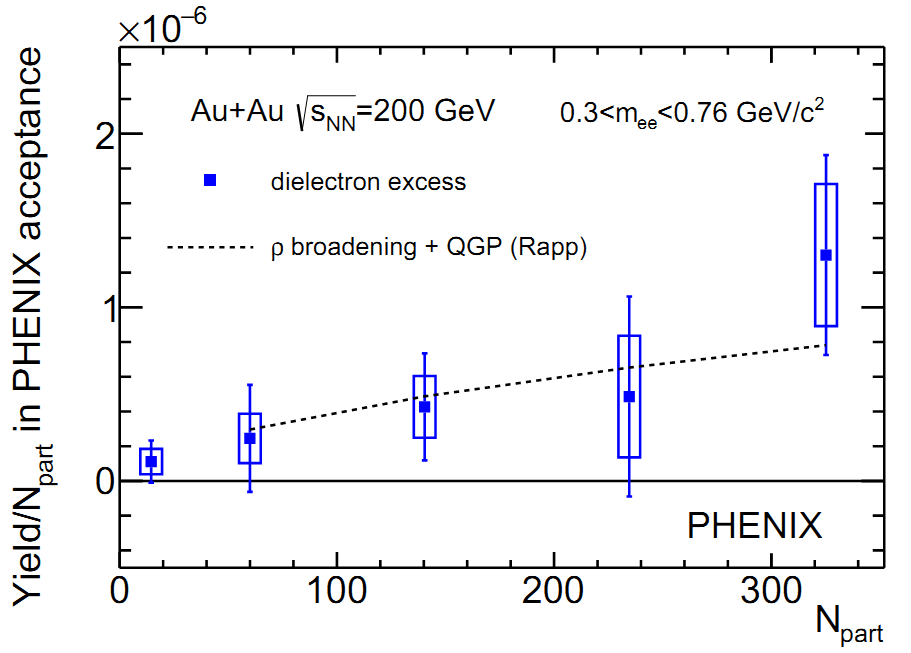
\includegraphics[width=1.0\textwidth]{introduction/PHENIX_LMexcess_Yield.png} 
\caption{Centrality dependence of the dielectron excess (data - cocktail) compared to the thermal radiation from hadronic medium and QGP phase from the model calculations of Rapp.\label{PHENIX_LMRexcessYield}}
\end{minipage}
\end{figure}

\subsection{STAR Experiment}
The Solenoidal Tracker at RHIC (STAR)~\cite{STARdet}, discussed in Sec.~\ref{stardet}, is a general purpose detector located at 6 o'clock of RHIC ring. The dielectron program is enabled with the barrel time-of-flight system upgrade. A (94.6 $\pm$ 1.9)\% overall electron purity can be achieved in Au + Au minimum-bias collisions at $\sqrt{s_{NN}}$ = 200 GeV~\cite{STAR:dielectron1}, combining the Time Projection Chamber (TPC) and Time of Flight (TOF) sub-detectors. 

STAR reported the dielectron measurements within STAR acceptance in $p$ + $p$ collisions at $\sqrt{s_{NN}}$ = 200 GeV using the data taken in year 2009~\cite{STAR:dielectron0}, as shown in Fig.~\ref{STAR_pp200Spec}. Within the uncertainties, the data is consistent with the hadronic cocktail simulation. STAR also reported the dielectron measurements within STAR acceptance in Au + Au collisions at $\sqrt{s_{NN}}$ = 200 GeV using the data taken in years 2010 and 2011~\cite{STAR:dielectron1:PRL,STAR:dielectron1}. The efficiency-corrected dielectron continuum in minimum-bias data and the comparisons with hadronic cocktail simulation and theoretical calculations incorporating broadened $\rho$ spectral functions~\cite{broaden0,broaden1,broaden4,broaden:PHSD0,broaden:PHSD1} (``effective many-body theory model'' and ``microscopic transport dynamic models'') are shown in Fig.~\ref{STAR_AuAu200Spec}. A significant enhancement compare to the hadronic cocktail in LMR ($M_{ee}<$ 1 GeV/$c^{2}$) can be observed, and the enhancement factor in 0.30 $<M_{ee}<$ 0.76 GeV/$c^{2}$ ($\rho$-like region) is 1.76 $\pm$ 0.06 (stat.) $\pm$ 0.26 (sys.) $\pm$ 0.29 (cocktail). The excess spectrum can be reasonably described by theoretical calculations incorporating broadened $\rho$ spectral function and QGP contribution from both Rapp and PHSD. Moreover, the excess in LMR can be consistently observed and described by the model calculations in differential measurements in various $p_{T}$ and centrality bins. The integrated excess yield in $\rho$-like region increases faster than $N_{part}$ scaling and follows a power-law scaling of $N_{part}$ ($\propto$$N_{part}^{1.44 \pm 0.10}$), indicating that the dielctron yield in $\rho$-like region is sensitive to the QCD medium dynamics. 

\begin{figure}[htbp]
\begin{minipage}[htbp]{0.50\linewidth}
\centering
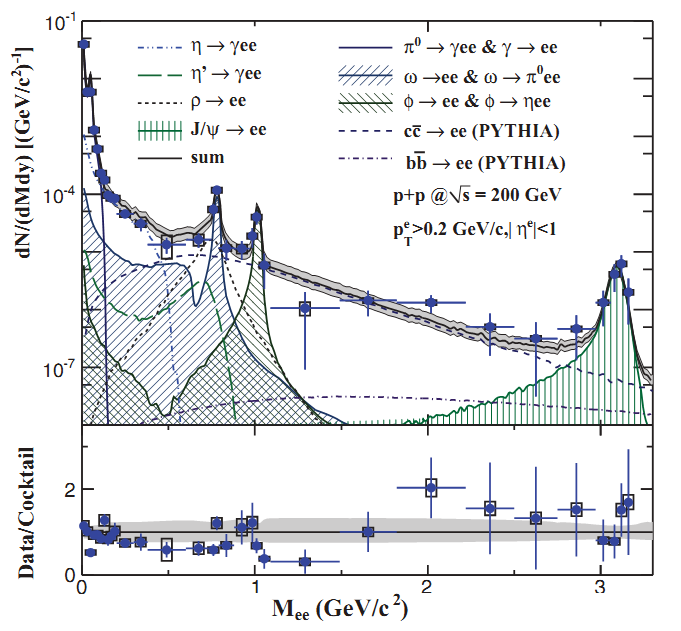
\includegraphics[width=1.0\textwidth]{introduction/STAR_pp200_spec.png}
\caption{(Top) The di-electron continuum after efficiency correction and hadronic cocktail simulation within STAR acceptance in $p$ + $p$ collisions at $\sqrt{s_{NN}}$ = 200 GeV (Bottom) The ratio of data over cocktail as a function of invariant mass. \label{STAR_pp200Spec}}
\end{minipage}
\hfill
\begin{minipage}[htbp]{0.48\linewidth}
\centering
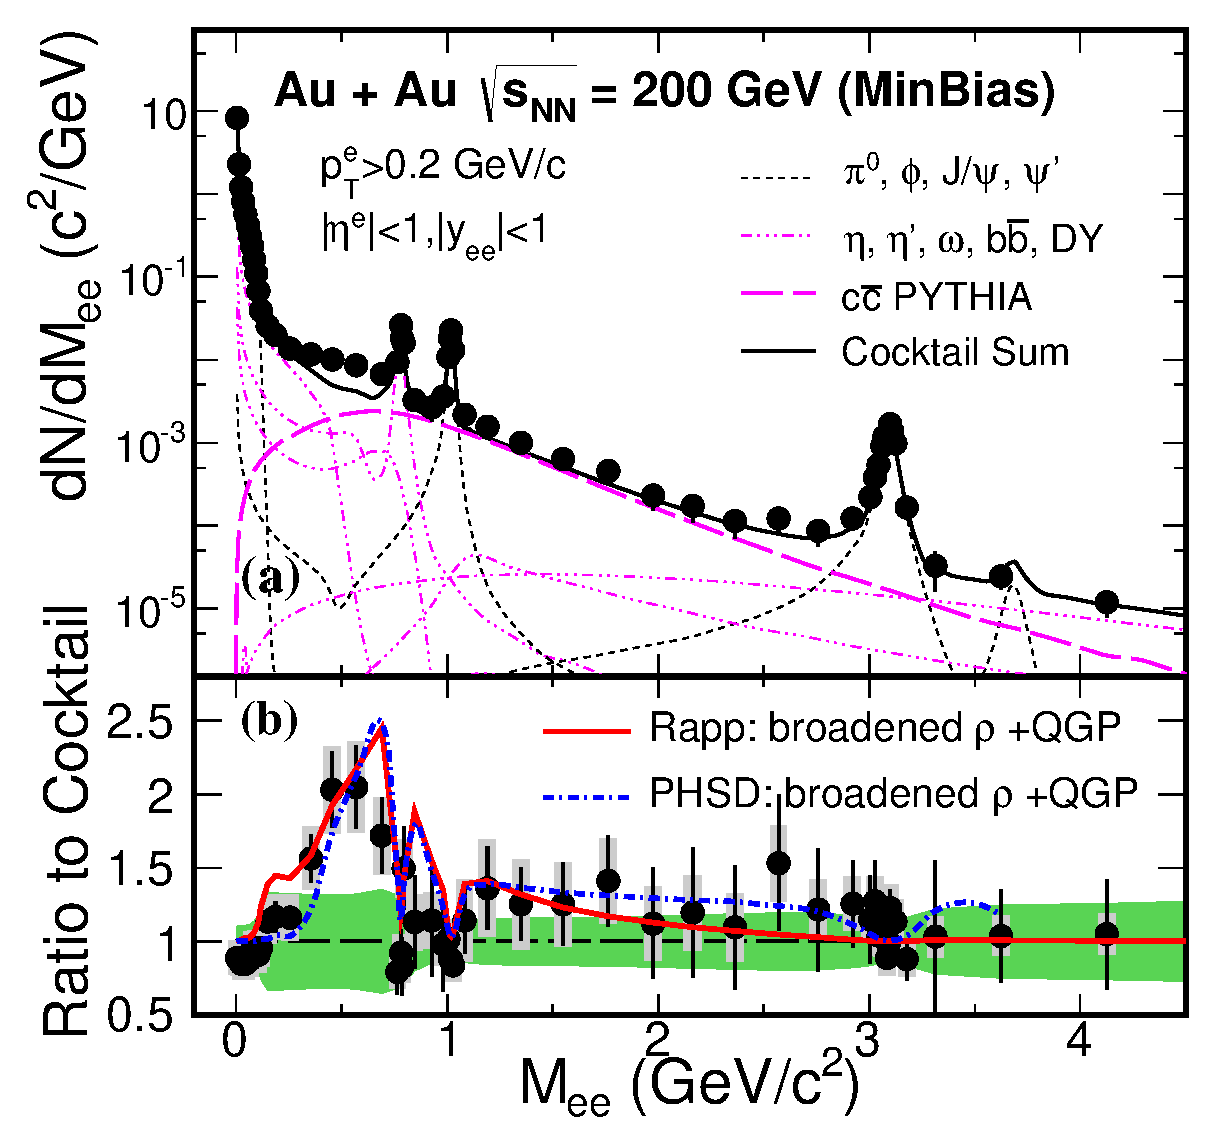
\includegraphics[width=1.0\textwidth]{introduction/STAR_AuAu200_spec.eps} 
\caption{(Top) The invariant mass spectrum from Au + Au minimum-bias collisions at $\sqrt{s_{NN}}$ = 200 GeV compared to a hadronic cocktail simulation. (Bottom) The ratio of data over cocktail as a function of invariant mass and model calculations.\label{STAR_AuAu200Spec}}
\end{minipage}
\end{figure}

\begin{figure}[htbp]
\begin{minipage}[htbp]{0.49\linewidth}
\centering
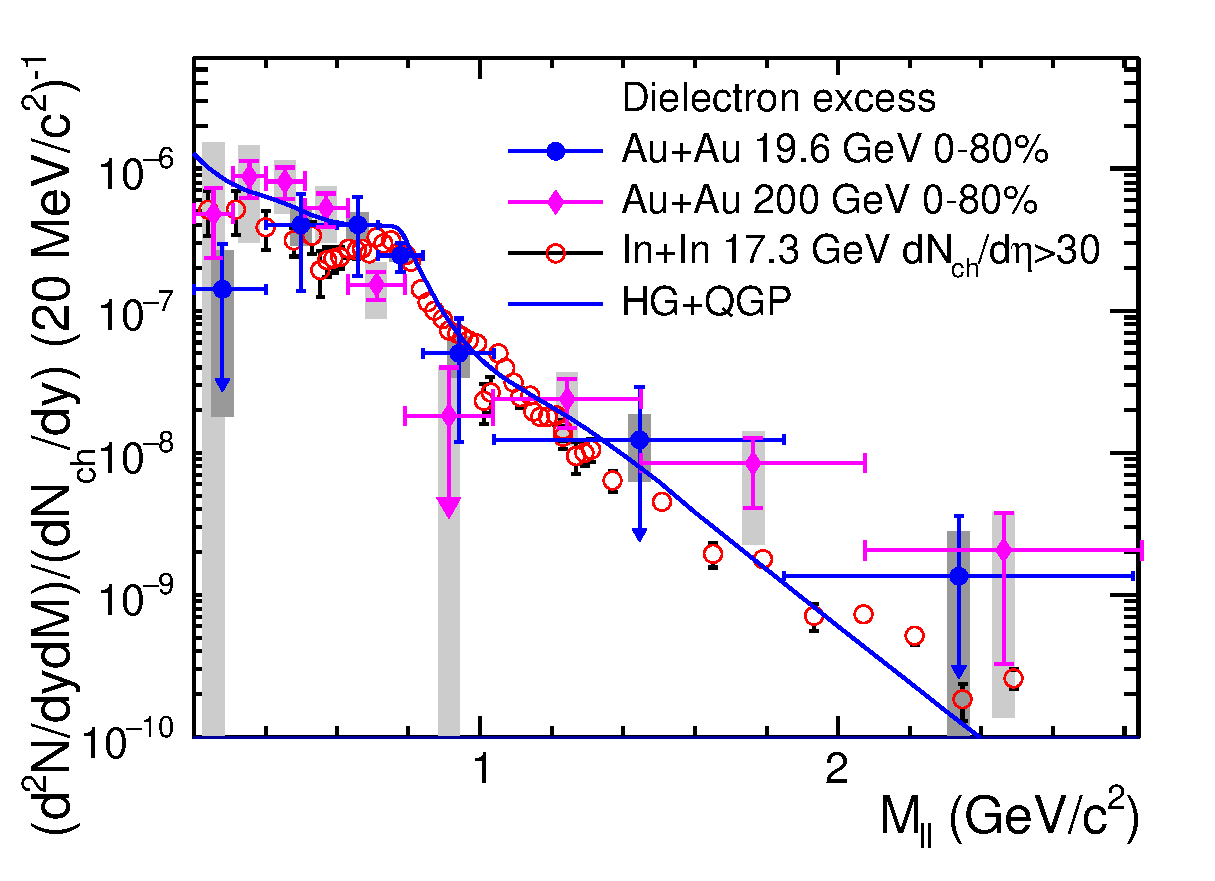
\includegraphics[width=1.0\textwidth]{introduction/STAR_Acc_ExcessSpec.eps}
\caption{The $dN_{ch}/dy$ normalized acceptance-corrected excess dielectron invariant mass spectra in Au + Au collisions at $\sqrt{s_{NN}}$ = 19.6 and 200 GeV, together with that of NA60 in In + In at $\sqrt{s_{NN}}$ = 17.3 GeV. A theoretical model calculation is also added for comparison.\label{STAR_AccExcessSpec}}
\end{minipage}
\hfill
\begin{minipage}[htbp]{0.49\linewidth}
\centering
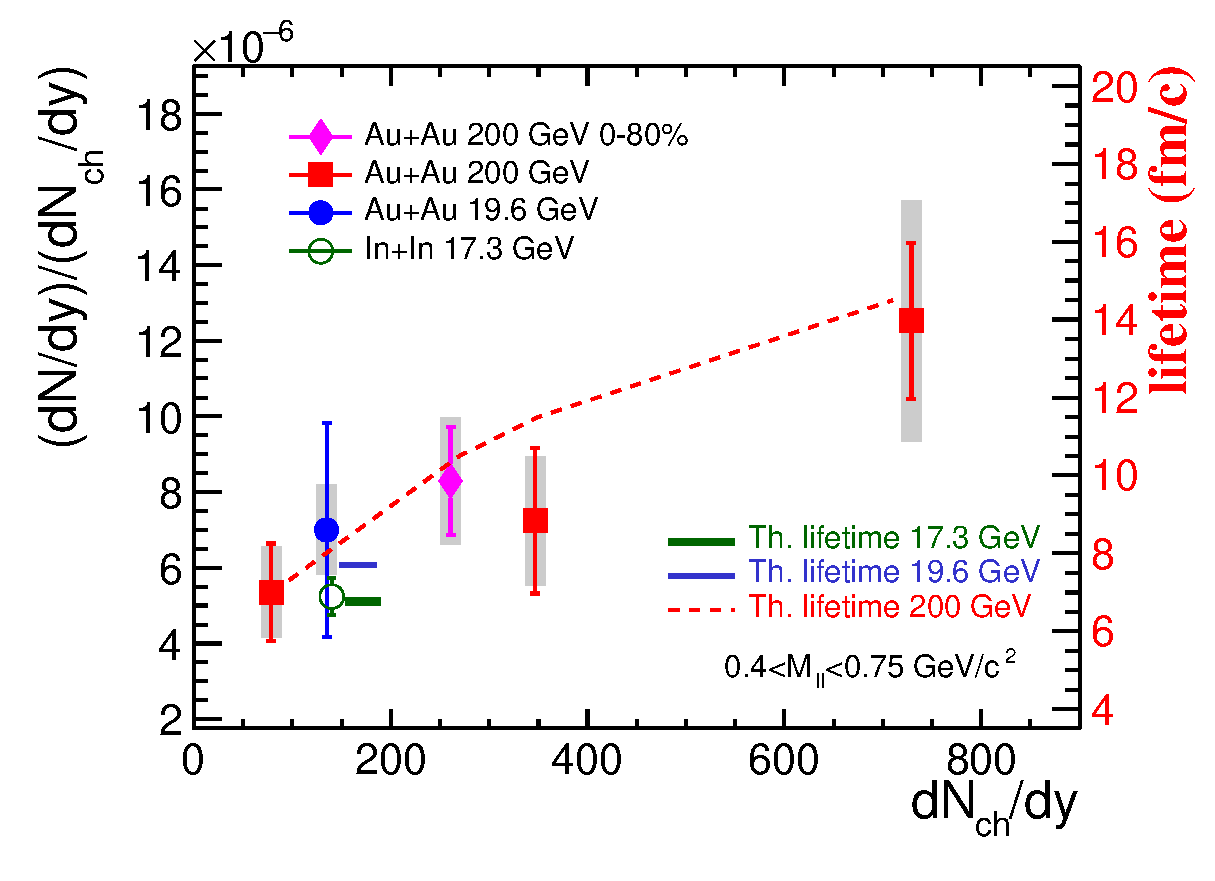
\includegraphics[width=1.0\textwidth]{introduction/STAR_Integrated_ExcessYield.eps} 
\caption{Integrated yields of the normalized dilepton excesses for 0.4 $<M_{ll}<$ 0.75 $GeV/c^{2}$ as a function of $dN_{ch}/dy$ in different collision systems and energies. The theoretical lifetimes are shown as a dashed curve and two horizontal bars.\label{STAR_AccExcessYield}}
\end{minipage}
\end{figure}

To quantitatively study excess dileptons, STAR also measured the acceptance-corrected excess spectra for Au + Au collision at $\sqrt{s_{NN}}$ = 19.6 and 200 GeV, as shown in Fig.~\ref{STAR_AccExcessSpec}. The charged particle density ($dN_{ch}/dy$) normalized excess spectrum in Au + Au collisions at $\sqrt{s_{NN}}$ = 19.6 GeV is similar with that of NA60 in In + In collisions at $\sqrt{s_{NN}}$ = 17.3 GeV within uncertainty in the whole mass region, while the excess at $\sqrt{s_{NN}}$ = 200 GeV is higher than that at $\sqrt{s_{NN}}$ = 17.3 GeV in the LMR and IMR, but within 2$\sigma$ uncertainty. All of the excess spectra can be described by the same model calculation from Rapp incorporating a broadened $\rho$ spectral function and QGP thermal radiation contribution. To quantitatively compare the excess in the LMR, the integrated excess yield in 0.4 $<M_{ee}<$ 0.75 GeV/$c^{2}$ are calculated for Au + Au at $\sqrt{s_{NN}}$ = 19.6 and 200 GeV. The excess yield has a centrality dependence and increases from peripheral to central collisions at $\sqrt{s_{NN}}$ = 200 GeV, and the excess yield in most central Au + Au collisions at 200 GeV is larger than that in lower energies. These measurements might indicate the lifetime of the medium created in Au + Au central collisions at 200 GeV is longer than those in peripheral and/or low-energy collisions, which enhances the dilepton production from thermal radiation.
 
 \begin{figure}[htbp]
\centering
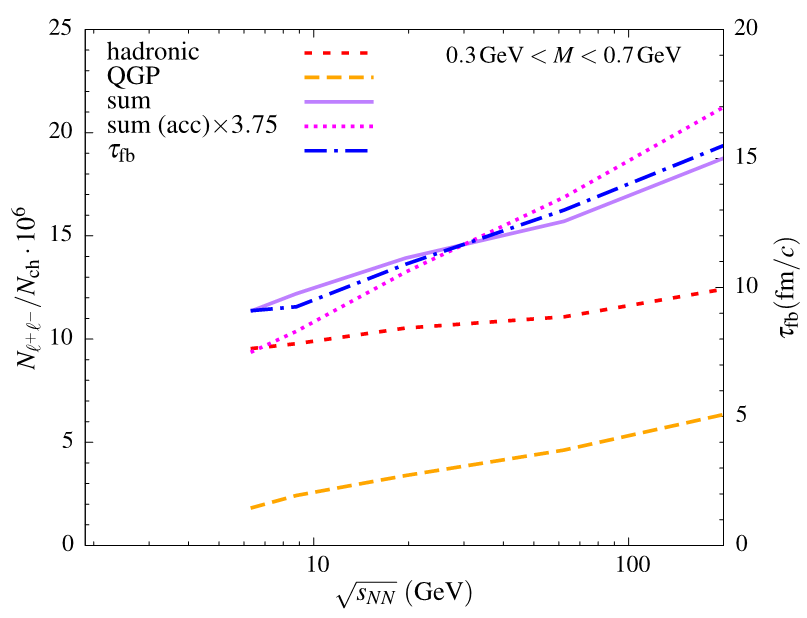
\includegraphics[keepaspectratio,width=0.6\textwidth]{introduction/norExcessYield_vs_energy.png}
\figcaption{Excess spectra in 0–10\% central AA collisions (A$\approx$200), integrated over the mass range $M_{ee}$ = 0.3-0.7 GeV/$c^{2}$, for QGP (dashed line) and in-medium hadronic (short-dashed line) emission and their sum (solid line). The underlying fireball lifetime (dot-dashed line) is given by the right vertical scale.}
 \label{lifetime}
\end{figure}

\section{Advantage of Dielectron Measurements in U + U Collisions at $\sqrt{s_{NN}}$ = 193 GeV}
 The Uranium nucleus is heavier than Gold nucleus, and the energy density created in U + U collisions at $\sqrt{s_{NN}}$ = 193 GeV is expected to be higher by about 20\% than that in Au + Au collisions at $\sqrt{s_{NN}}$ = 200 GeV~\cite{UUEnergyDensity}. The medium created in U + U collisions might have a longer lifetime compared with the Au + Au collisions. Recently, it is found in a model calculation that the charged particle multiplicity ($dN_{ch}/dy$) normalized dilepton excess yield in the low mass region is proportional to the lifetime of the hot, dense medium created in heavy-ion collisions at $\sqrt{s_{NN}}$ = 6 - 200 GeV~\cite{lifetime_cal}, as shown in Fig.~\ref{lifetime}. Thus it would be interesting to measure the normalized dielectron excess yields in U + U collisions and compare with that in Au + Au collisions.
  \chapter{Experimental Setup}

\section{Relativistic Heavy Ion Collider}
The Relativistic Heavy Ion Collider (RHIC) at Brookhaven National Laboratory (BNL), shown in Fig.~\ref{rhic_config}, is a versatile high energy collider~\cite{RHIC_Overview}. Since year 2000, RHIC has successfully collided $p$ + $p$, $p$ + Al, $p$ + Au, $d$ + Au, $^3$He + Au, Cu + Cu, Cu + Au, Au + Au, and U + U at different energies. The top  energy for the gold ions is 100 GeV/$u$ and that for protons is 250 GeV. A major scientific goal of  RHIC is to study the properties of hot, dense and strongly interacting quantum chromodynamics (QCD) matter created in the laboratory. Meanwhile, as the world-only polarized proton high energy collider, RHIC allows the experimental studies of nucleon's spin structure. Reviews of recent achievements and future of the RHIC spin program can be found in~\cite{RHIC_Spin}.

\begin{figure}[htbp]
\centering
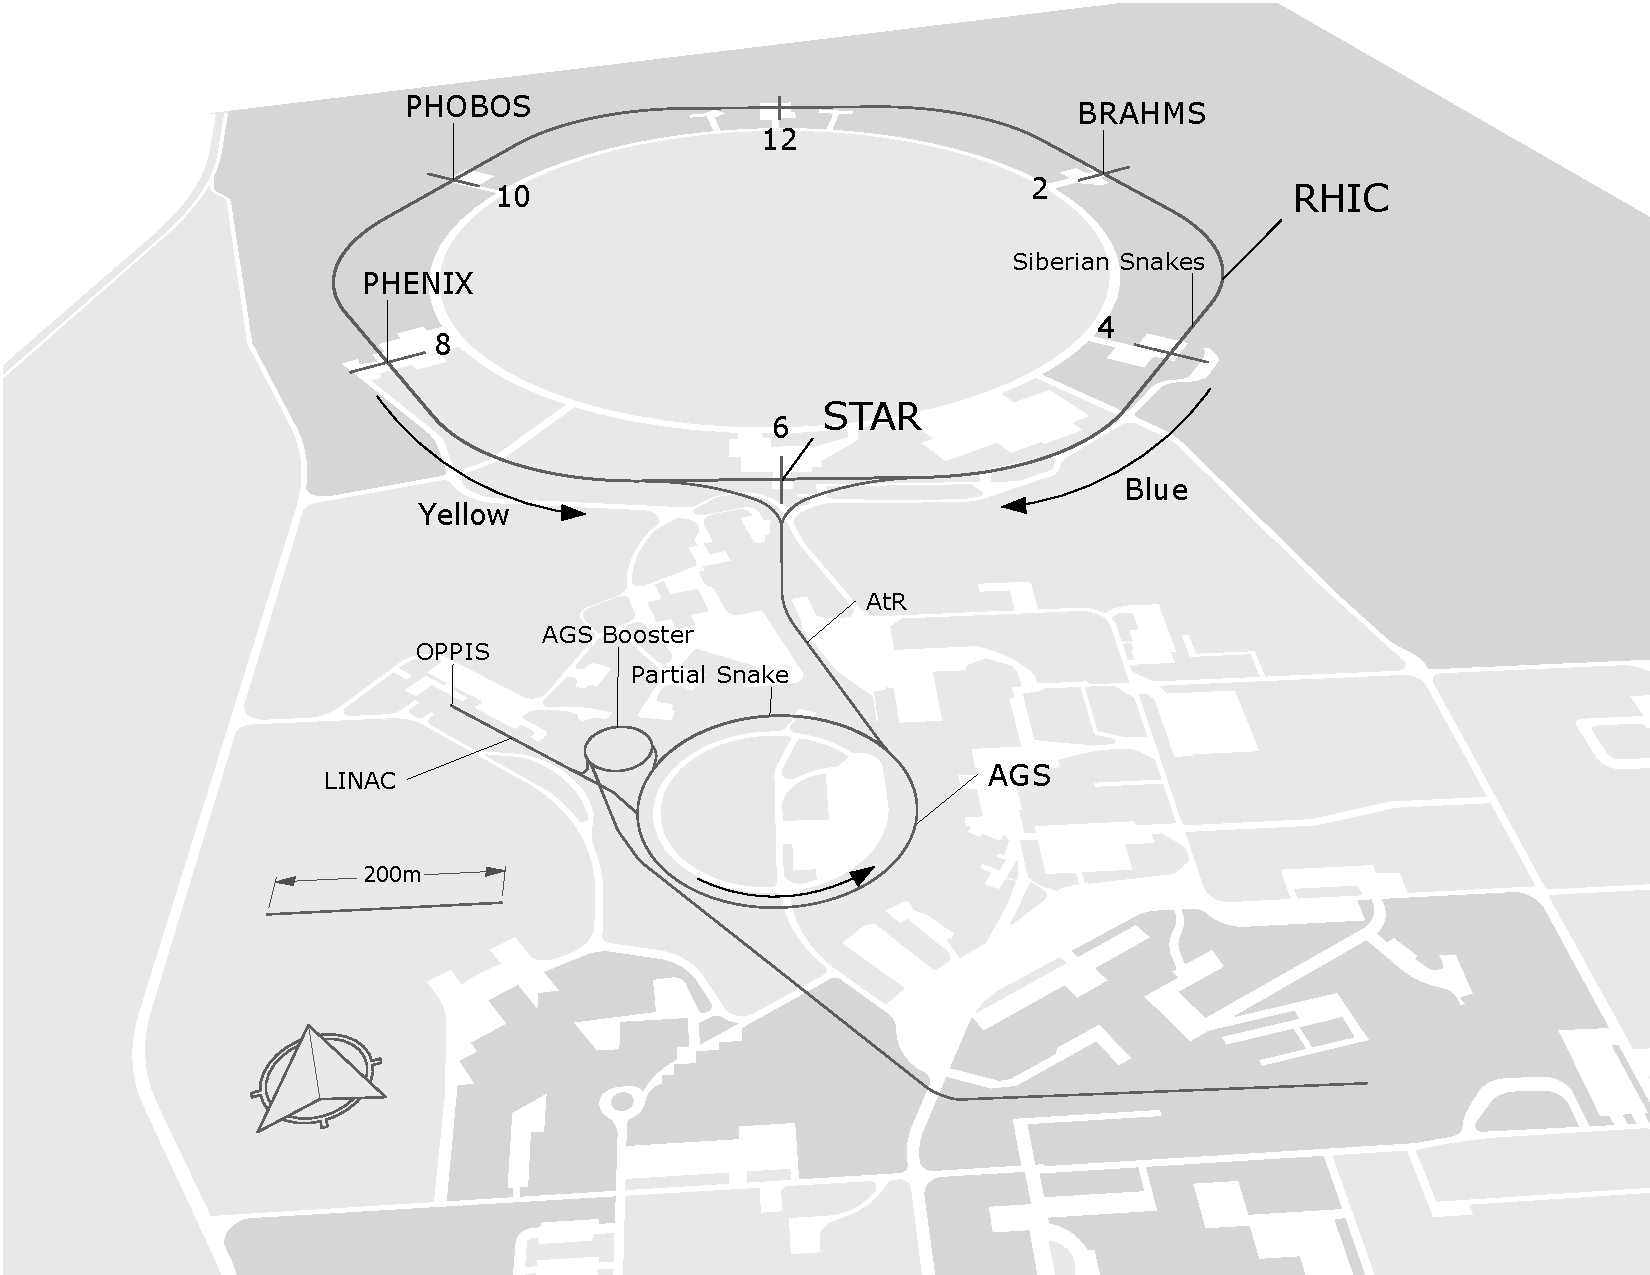
\includegraphics[keepaspectratio,width=0.85\textwidth]{rhic_star/RHIC_Configration.pdf}
\figcaption{The RHIC accelerator complex.}
 \label{rhic_config}
\end{figure}

The process of accelerating gold ions are show in Fig.~\ref{rhic_acc}. Negatively charged (Q = -1) gold ions from the pulsed sputter ion source are partially stripped of electrons in Tandem Van de Graaff, and accelerated to the energy of 1 MeV/$u$. The ions are stripped further (Q = +32) at the exit of the Tandem and then delivered to the Booster Synchrotron through a transfer line. The ions are accelerated to 95 MeV/$u$ in the Booster, and stripped again at the exit to achieve a charge state of Q = +77. The ions are then delivered to the Alternating Gradient Synchrotron (AGS) in 24 bunches. In the AGS, the ions beam are de-bunched, re-bunched to four bunches and accelerated to 10.8 GeV/$u$. The gold ions are fully stripped to the charge state of Q = +79 at the exit from the AGS. These four bunches, one bunch at a time, are injected to the RHIC ring through the AGS-to-RHIC beam transfer line. Once in RHIC, the ions are accelerated to 100 GeV/$u$ (typically, other energies are possible). The protons are accelerated in a different process. They are first accelerated to 200 MeV in a linear accelerator (Linac) before being delivered to the Booster, then to the AGS, and finally to RHIC ring.

RHIC consists of two 3.8 km quasi-circular concentric rings on a common horizontal plane, one (``Bule Ring'') for clockwise and the other (``Yellow Ring'') for counter-clockwise. There are six interaction points on RHIC rings, among which are located four experiments, called STAR at 6 o'clock, PHENIX at 8 o'clock, PHOBOS at 10 o'clock and BRAHMS at 2 o'clock. PHOBOS and BRAHMS experiments decommissioned in 2005 and 2006, respectively, after completing their physics goals. While the STAR and PHENIX experiments are still operating as of today.

An upgrade to Electron Ion Collider (EIC) known as eRHIC~\cite{eRHIC}, focused on the structure and interactions of gluon-dominated matter~\cite{EIC_Physics}, is being planed. The new facility will deliver electron-nucleon luminosity of 10$^{33}$-10$^{34}$ cm$^{-2}$sec$^{-1}$ for collisions of 15.9 GeV polarized electrons on either 250 GeV polarized protons or 100 GeV/$u$ heavy ion beams. The facility will also be capable of providing an electron beam energy of 21.2 GeV, at reduced luminosity. 

\begin{figure}[htbp]
\centering
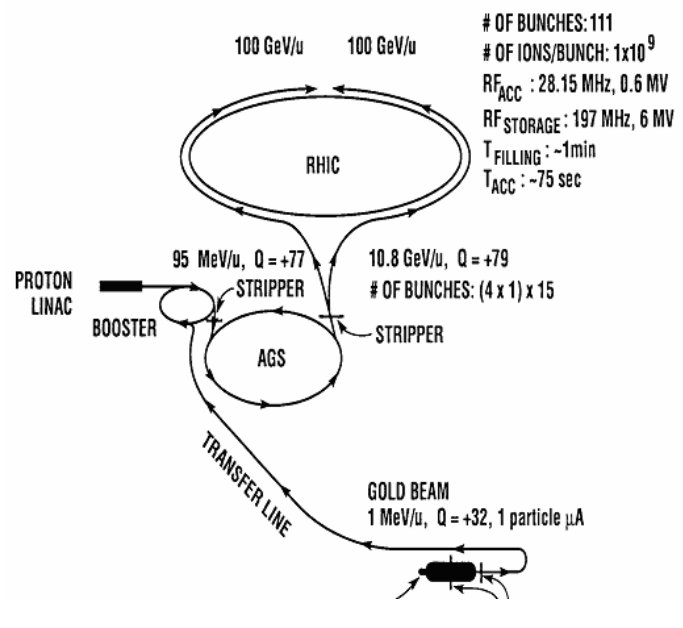
\includegraphics[keepaspectratio,width=0.7\textwidth]{rhic_star/RHIC_AccGold.png}
\figcaption{RHIC acceleration scenario for Au beam~\cite{RHIC_Configuration}.}
 \label{rhic_acc}
\end{figure}

\section{STAR Detector}
\label{stardet}
The Solenoidal Tracker at RHIC (STAR) ~\cite{STARdet}, composed of several sub-detector systems, is a multi-purpose particle detector. The large and uniform acceptance (0$<\phi<$ 2$\pi$, $|\eta|<$ 1) of the STAR detector, makes it well suited for event-by-event characterization of high charged particle multiplicity heavy-ion collisions. Figure~\ref{star} shows the layout of the STAR detector complex. The center of STAR serves as the original point. The $x$ direction is pointing to the south and the $y$ direction is pointing up (away from the earth surface). The $z$ direction is the beam pipe direction with the west direction as being positive. The whole system except the Muon Telescope Detector (MTD) is enclosed in a homogeneous magnetic filed generated by a solenoidal magnet. The magnetic field direction is parallel to the beam pipe and the maximum magnetic field is $|B_{z}|$ = 0.5 T. STAR can be operated in full field, reverse full field and half field magnetic field configurations.

\begin{figure}[htbp]
\centering
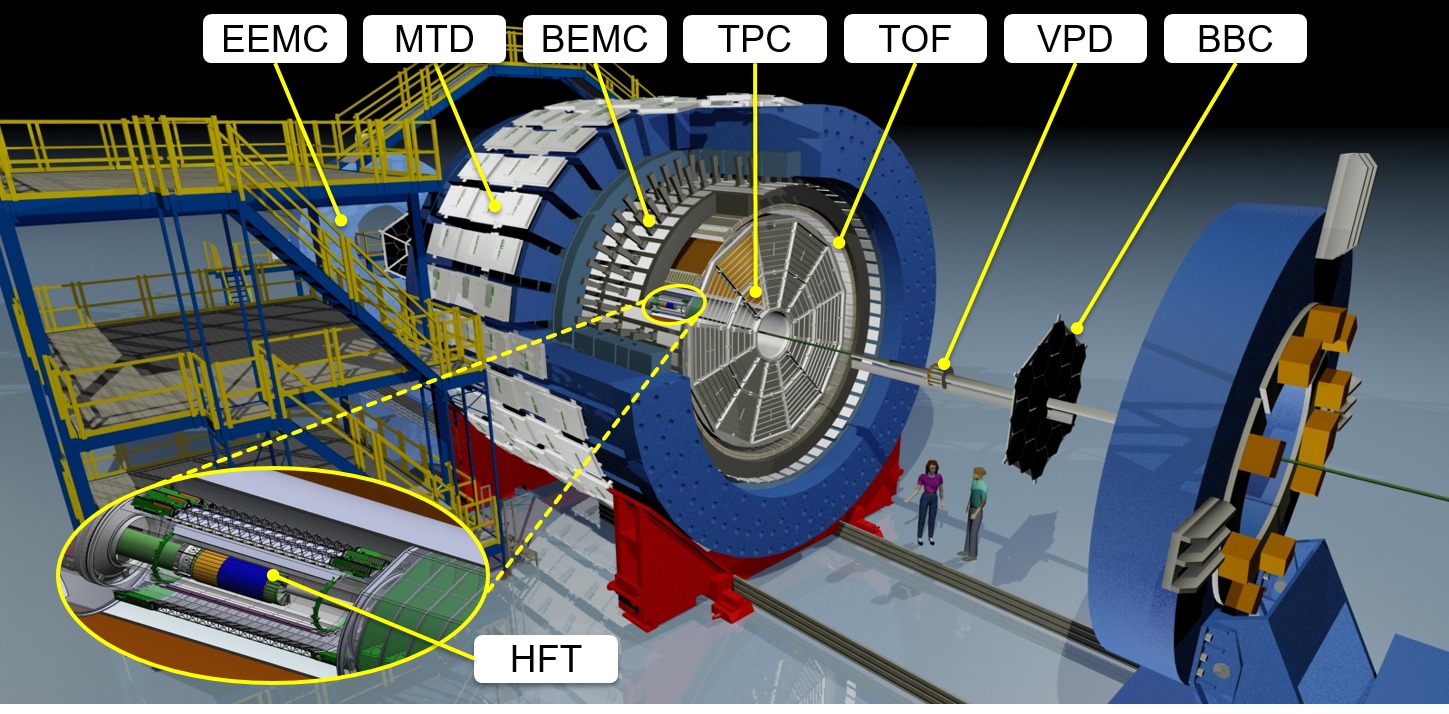
\includegraphics[keepaspectratio,width=1\textwidth]{rhic_star/STAR.png}
\figcaption{Perspective view of the STAR detector.}
 \label{star}
\end{figure}

Charged particle tracking close to the interaction region is accomplished by the Heavy Flavor Tracker (HFT)~\cite{HFTdet}. The HFT was completely installed before 2014 physics run, and successfully collected $\sim$1.2 billion minimum-bias Au + Au events in the 2014 run and $\sim$1 billion $p$ + $p$ , $\sim$0.6 billion $p$ + Au events in the 2015 run. The HFT consists of four cylindrical silicon detector layers and covers $|\eta|<$ 1.2. Two innermost silicon PiXeL detector (PXL) layers are the first application of the state-of-the-art thin Monolithic Active Pixel Sensors (MAPS) technology in a collider environment. The outermost layer is the Silicon Strip Detector while the Intermediate Silicon Tracker (IST) layer sits in the middle of the HFT. The high spatial resolution of the tracker allows us to reconstruct the secondary decay vertices of short-lived particles, such as the D$^{0}$, D$^{+/-}$, D$_{s}$ mesons. A preliminary measurement of the D$^{0}\rightarrow$ K$\pi$ production in Au + Au at $\sqrt{s_{NN}}=$ 200 GeV using 125M minimum-bias data collected in year 2014 is shown in Fig.~\ref{D0signal}~\cite{D0plot}. The combinatorial background is suppressed by $\sim$4 orders of magnitude achieved by the HFT. 

\begin{figure}[htbp]
\centering
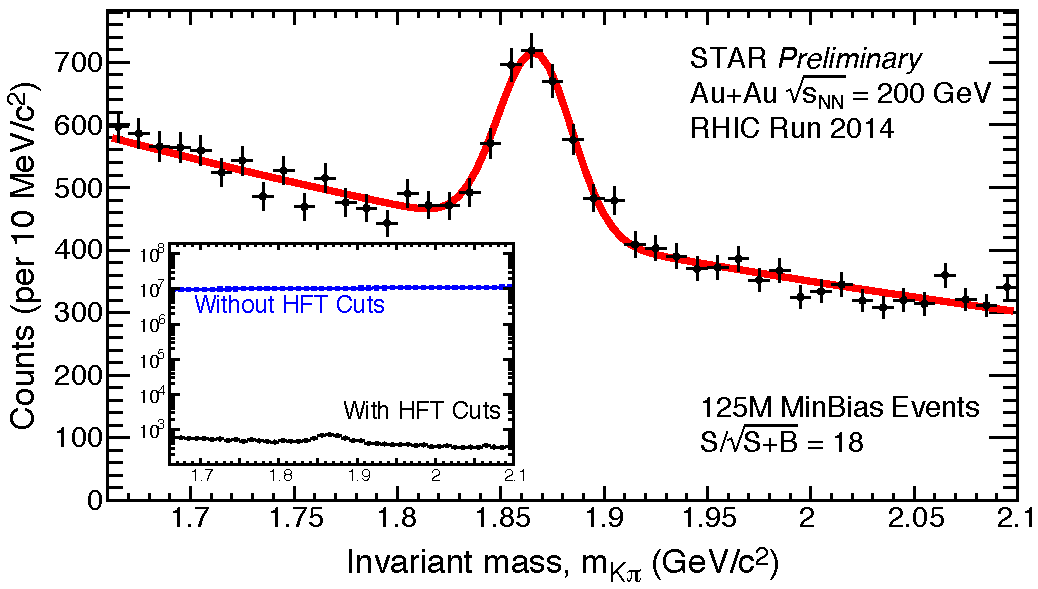
\includegraphics[keepaspectratio,width=0.8\textwidth]{rhic_star/D0_Signal.pdf}
\figcaption{D$^{0}\rightarrow$ K$\pi$ production in Au + Au at $\sqrt{s_{NN}}=$ 200 GeV using 125M  minimum-bias data collected in year 2014~\cite{D0plot}. The insert plot shows the suppression of combinatorial background by $\sim$4 orders of magnitude achieved by the HFT.}
 \label{D0signal}
\end{figure}

The Time Projection Chamber (TPC)~\cite{TPCdet} is the main tracking device in STAR, whose inner and outer field cages are located at radial distance of 50 and 200 cm respectively from the beam axis. The TPC is 4.2 meters long and it covers a pseudo-rapidity range $|\eta|<$ 1.8 and full azimuthal. The TPC provides charged particle tracking, momentum and ionization energy loss ($dE/dx$) measurements for particle identification. The TPC is surrounded by the Time-of-Flight (TOF)~\cite{TOFdet} detector which covers $|\eta|<$ 0.9 and complete azimuthal symmetry. The TOF measures the charged particle velocity and enable us to reject the slow hadron from electrons, opening an opportunity for dielectron analysis at STAR. Following the TOF is the Barrel ElectroMagnetic Calorimeter (BEMC)~\cite{BEMCdet}. The BEMC (0$<\phi<$2$\pi$, $|\eta|<$ 1) is used to trigger on and measure high transverse momentum electrons, photons. In addition, the BEMC also provides prompt charged particle signals essential to discriminate against pileup tracks in the TPC in high luminosity $p$ + $p$ collisions. Outside of the BEMC is the STAR magnet system. The magnetic coils and steels can reject most hadrons while the cross-section of muon in the magnet is small. The muons can penetrate the coils and steels and reach the MTD~\cite{MTDdet}, which is located at the outermost of STAR. The MTD system was fully installed in early 2014 and it covers about 45\% in azimuthal within $|\eta|<$ 0.5. The MTD can trigger on and identify muons based on its precise timing and modest position resolution.

Along the beam axis, there are three fast trigger detectors: Beam Beam Counter (BBC)~\cite{BBCdet}, Vertex Position Detector (VPD)~\cite{VPDdet}, Zero Degree Calorimeter (ZDC)~\cite{ZDCdet}.  The BBC consists of two collections of four scintillator annuli centered around the beam pipe, each located 3.74 m from the interaction region. The two inner (18 channels) and two outer (18 channels) annuli together cover a pseudo-rapidity range of ~2.1 $<|\eta|<$ 5.0, and there is a slight overlap between the inner and outer annuli. The BBC acts as a main detector in the $p$ + $p$ minimum-bias trigger. The minimum-bias trigger requires at least one hit in the two inner annuli of each side coincidentally. This trigger corresponds to a $p$ + $p$ cross section of  $\sim$26.1 $\pm$ 0.2 (stat.) $\pm$ 1.8 (sys.) mb, 87$\pm$8\% of the total none singly diffractive cross section. The VPD consists of two assemblies, and each assembly is composed of 19 channels (units) while only 16 channels are used for STAR trigger input. The two assemblies of the VPD are symmetrically located at a distance of 5.7 m with respect to the interaction region and the VPD covers a pseudo-rapidity of 4.24 $<|\eta|<$ 5.1. The VPD is fully integrated into the STAR trigger system and provides the primary input to the minimum-bias trigger in nucleus-nucleus collisons. The precise timing information from the VPD detector channels is used both in online ($\sim$150 ps in $\sqrt{s_{NN}}$ = 200 GeV Au + Au) and offline ($\sim$30 ps in $\sqrt{s_{NN}}$ = 200 GeV Au + Au) to measure the $z$ position of primary vertex and provide ``start time'' for the TOF and MTD. The two assemblies of ZDC are directly in line with the STAR beam pipe, located 18 m from the interaction point. The ZDC is used for measuring the energy in neutral particles surviving the heavy-ion collisons. The more overlap of ions, the less neutral particles survive from the collisions, and the smaller signal in the ZDC. This makes the ZDC sensitive to the centrality of the collisions. Each experiment at RHIC has a complement of ZDCs for triggering, monitoring luminosity, and cross-calibrating the centrality triggering between experiments.

In the next few sections, we will focus on the TPC and TOF which play a direct role in this dielectron analysis.

\subsection{Time Projection Chamber}
\label{detector:TPC}

The Time Projection Chamber (TPC) is the central element of STAR, and it records the charged particle tracks, momenta and ionization energy loss for particle identification. At the time it was built, the STAR TPC was the largest TPC in the world with a 4.2 m long and 4 m in diameter.  It sits in the STAR solenoidal magnet which produces a maximum 0.5 T magnetic field,  allowing for the momenta measurement.

Figure~\ref{tpccage} shows the schematic view of the STAR TPC. The TPC is an empty volume of P10 (90\% Ar + 10\%CH$_{4}$) gas regulated at 2 mbar above atmospheric pressure in a uniform electric field of $\sim$135 V/cm which is along z direction and defined by a thin conductive Central Membrane (CM, held at -28 kV) at the center of  the TPC, concentric field-cage cylinders and the readout end caps (held at ground potential). The P10 gas has long been used in TPCs with advantage of a fast drift velocity peaking at a low electric field. Operating on the peak of the velocity curve makes the drift velocity stable and insensitive to the small variations in temperature and pressure. The transverse diffusion and longitudinal diffusion at 0.5 T are about $\sigma_{T}$ = 3.3 mm (230 $\mu$m/$\sqrt{cm}$) and $\sigma_{L}$ = 5.2 mm (360 $\mu$m/$\sqrt{cm}$), respectively, after drifting the full length of TPC. The longitudinal diffusion width sets the scale for the resolution of the tracking system in the drift direction.

\begin{figure}[htbp]
\centering
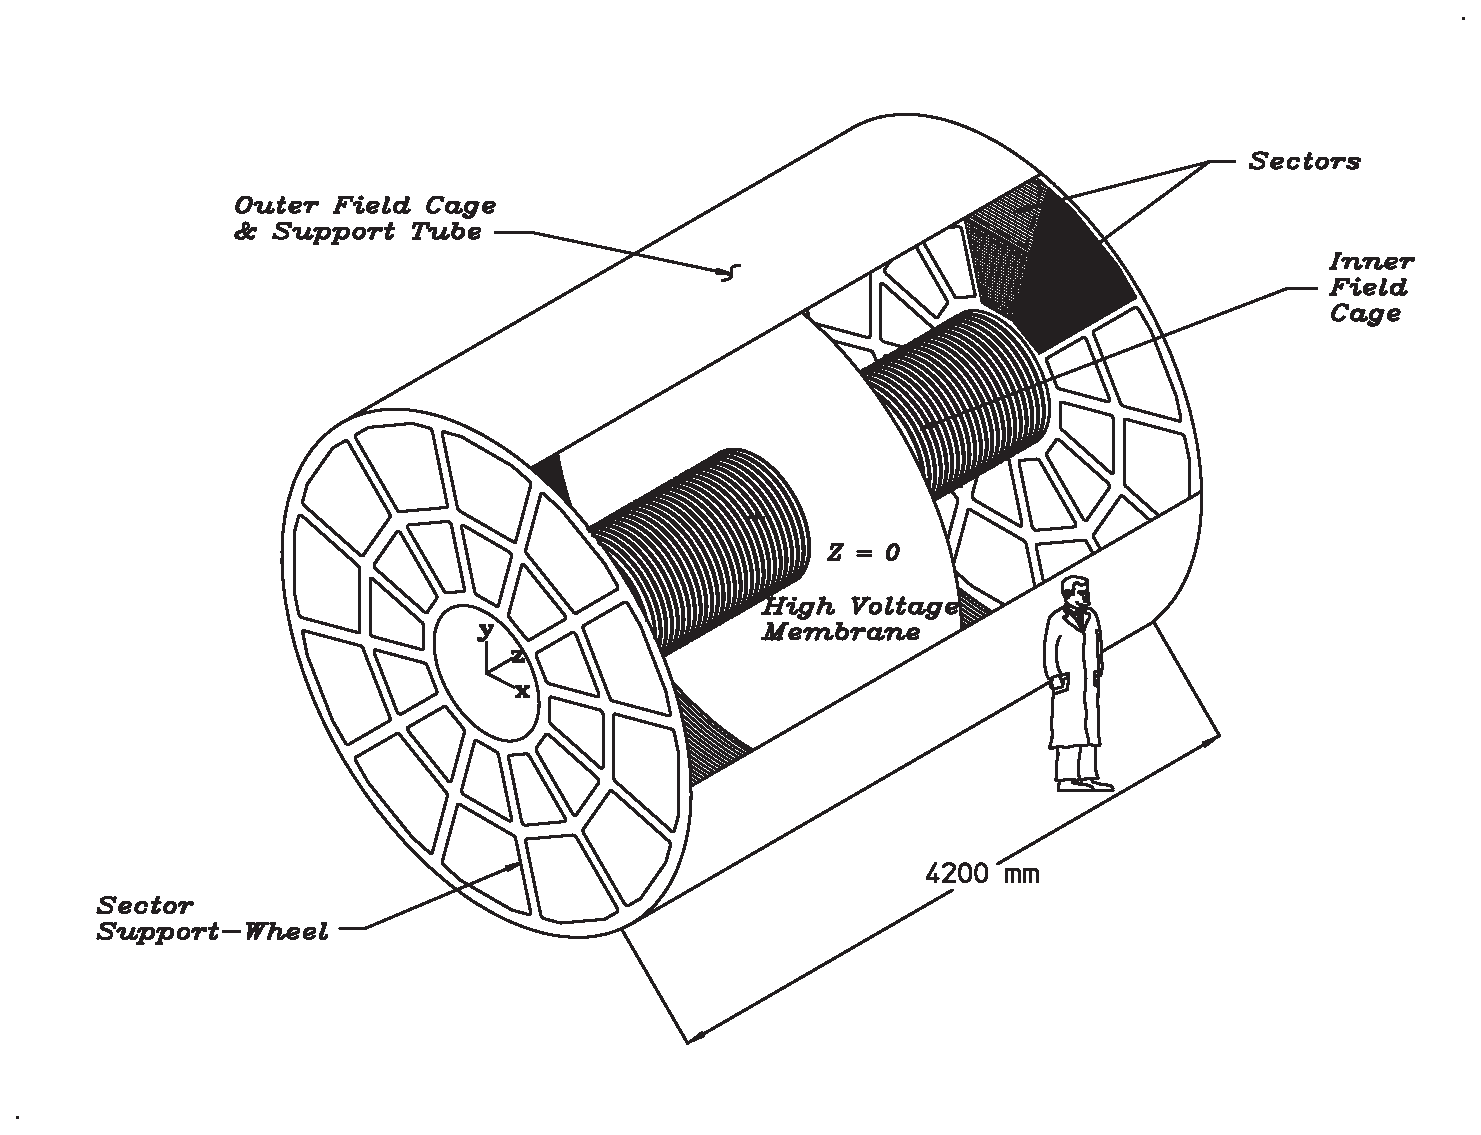
\includegraphics[keepaspectratio,width=0.9\textwidth]{rhic_star/tpcman.eps}
\figcaption{The schematics of the STAR TPC.}
 \label{tpccage}
\end{figure}

There are 12 sectors with 45 pad rows, arranged as on a clock face, in each readout end cap. Each sector is then divided into an outer and inner sub-sector as shown in Fig.~\ref{padplane}. The outer sub-sector has a continuous pad coverage to optimize the $dE/dx$ resolution and tracking resolution. The inner sub-sector with smaller pads, located at the region of highest track density, is optimized for good two-hit resolution. The use of separate pad rows instead of continuous pad coverage for inner sub-sector is due to the constraint imposed by the available packing density of the front end electronics channels on that time.

\begin{figure}[htbp]
\centering
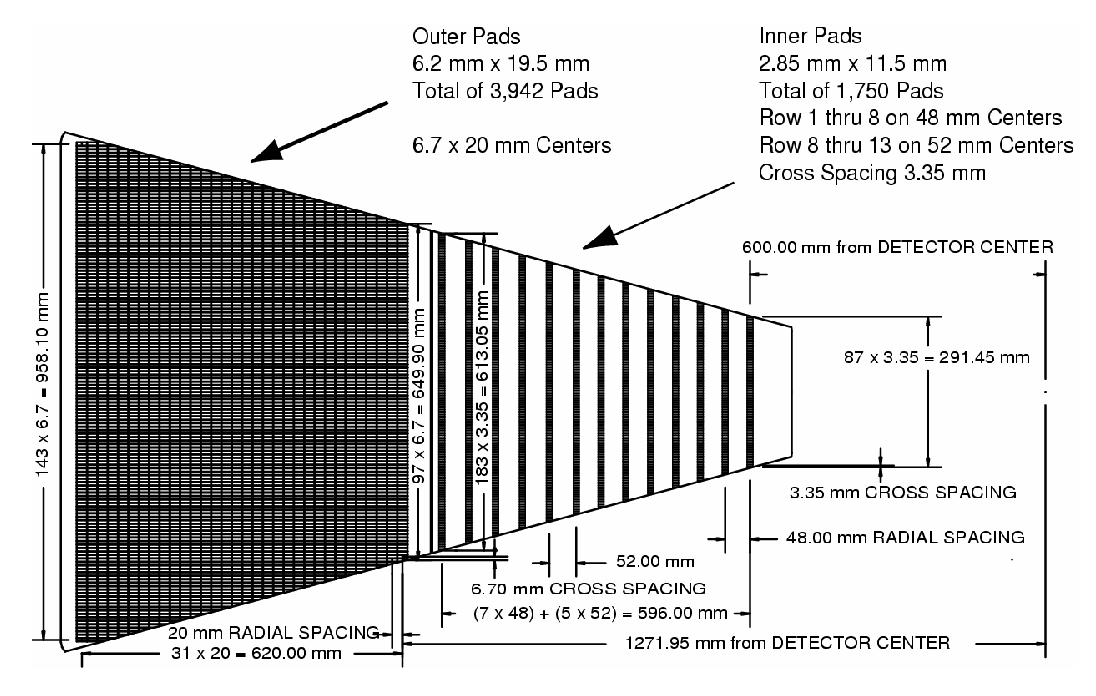
\includegraphics[keepaspectratio,width=0.8\textwidth]{rhic_star/padplane.eps}
\figcaption{ The anode pad plane with one full sector shown. The inner subsector is on the right and it has small pads arranged in widely spaced rows. The outer subsector is on the left and it is densely packed with larger pads.}
 \label{padplane}
\end{figure}

\begin{figure}[htbp]
\centering
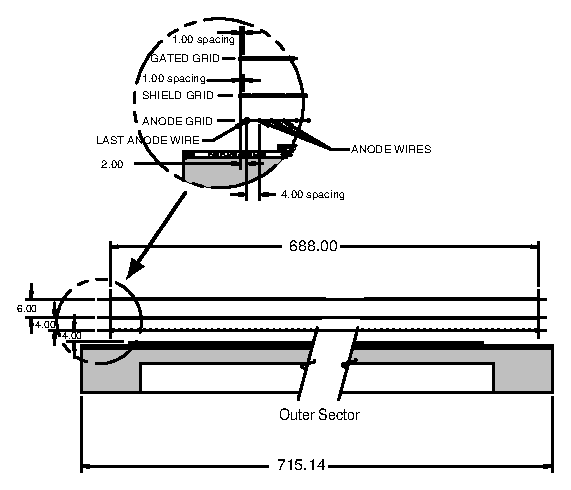
\includegraphics[keepaspectratio,width=0.8\textwidth]{rhic_star/outer_wires.eps}
\figcaption{ A cut-away view of an outer sub-sector pad plane. The cut is taken along a radial line from the center of the TPC to the outer field cage so the center of the detector is to the right. The figure shows the spacing of the anode wires relative to the pad plane, the ground shield grid, and the gated grid. The bubble diagram shows additional detail about the wire spacing. The inner subsector pad plane has the same layout except the spacing around the anode plane is 2 mm instead of the 4 mm shown here. All dimensions are in millimeters.}
 \label{mwpc}
\end{figure}

As charged particles pass through the TPC volume, they ionize the working gas along their path, releasing electrons and positive ions. The electrons drift toward the end cap and are collected by the Multi-Wire Proportional Chambers (MWPC). The MWPC is composed of a pad plane and three wire planes: a gating grid, a ground pane, and anode wires, shown in Fig.~\ref{mwpc}. The gating grid is ``close'' when the wires are alternately biased $\pm$75 V. Thus it blocks the entry of electron from TPC volume into MWPC and positive ions produced in MWPC into TPC volume. The gating grid is ``open'', biasing the wires to the same potential (typically -110 V), when recording the collision event. The positive ions are too slow to escape during the open period and get captured during the closed period. Once the electrons enter the MWPC, much more electrons are produced through avalanche in the high field inducing a signal on the readout plane. These induced signals  are used for tracing the position of ionization clusters along the charged particle tracks. The clusters are found separately in the $x$-$y$ plane ($r$-$\phi$ plane) and in z direction. The $x$ and $y$ coordinates of a cluster are determined by the charge measured on adjacent pads in a single pad row while the $z$ coordinate is determined by measuring the drift time of a cluster from the original point to the anodes on the endcap multiplying the average drift velocity (typically $\sim$5.45 cm/$\mu$s, but calibrated every few hours to account for atmospheric pressure variations by using artificial tracks created by lasers beams~\cite{TPClaser}). The particle tracks are then reconstructed from the individual clusters (hits) found in the TPC and the reconstruction is achieved with a Kalman filter routine. The resulted track collection from the TPC is combined with any other available tracking detector reconstruction hits and then refit. The reconstructed tracks are called global tracks. The primary interaction vertex is fit from the global tracks with at least ten hits. The Distance of Closest Approach (dca) to the fit primary vertex is calculated for each global track. Iterations are made such that global tracks with dca $>$ 3 cm are excluded from subsequent primary vertex fitting. The vertex resolution is inversely proportional to the square root of the number of tracks used in the calculation and can reach 350 $\mu$m when there are more than 1000 tracks. The tracks (global tracks with dca $<$ 3 cm) originated from the primary vertex are refit including the primary vertex to improve the momentum resolution, so called primary tracks. The momentum resolution of primary track in $p$ + $p$ collisions is approximately $\delta p_{T}/p_{T} \approx$ 1\% + 0.5\% $\times$ $p_{T}$.

Particle identification can be realized in the TPC through the $dE/dx$. The mean rate of $dE/dx$ of a charged particle passing trough the TPC can be described by the Bichsel function~\cite{Bichsel}. Different particle species with the same momentum may result in different $dE/dx$. The $dE/dx$ is extracted from the energy loss measured on up to 45 padrows. However, the mean $dE/dx$ is impossible to be accurately measured due to the ionization fluctuations and finite track length over the energy loss measured. Therefore, the most probable energy loss is measured by truncating the largest 30\% ionizations clusters. The typical resolution of $dE/dx$ in Au + Au collisions is $\sim$8\%, which makes the $\pi/K$ separation up to p $\sim$0.7 GeV/$c$ and ($\pi,K)/p$ separation up to p $\sim$1.1 GeV/$c$.

\subsection{Time of Flight}

The full barrel Time-of-Flight (TOF), based on the Multi-gap Resistive Plate Chamber (MRPC)~\cite{STARTOFmrpc0}, was completely installed in year 2010. The MRPC technology was first developed by the ALICE group~\cite{ALICETOFmrpc} to provide a cost-effective solution for large area Time-of-Flight coverage. The barrel TOF, covering $|\eta|<$ 0.9 and 2$\pi$ azimuthal, is composed of 120 trays, with 60 on east side and 60 on west side. Each tray consists of 32 single-end readout MRPC modules, whose structure is shown in Fig.~\ref{tofmrpc}. The MRPC module consists a stack of floating resistive plates with a series of uniform gas gaps (220 $\mu$m) defined by a nylon monofilament fishing line. The active size of the MRPC module is 61 $\times$ 200 mm$^{2}$. The module has 6 readout pads while each pad has an area of 63 $\times$ 31.5 mm$^{2}$. The interval between two pads is 3 mm wide. The first beam test for the MRPC module at CERN PS-T10 test beam facility using 7 GeV/$c$ pion beam resulted in 65 ps time resolution with greater than 95\% detection efficiency and capability of working at high event rate 500 Hz/cm$^{2}$ ~\cite{STARTOFmrpc0, STARTOFmrpc1}.


\begin{figure}[htbp]
\centering
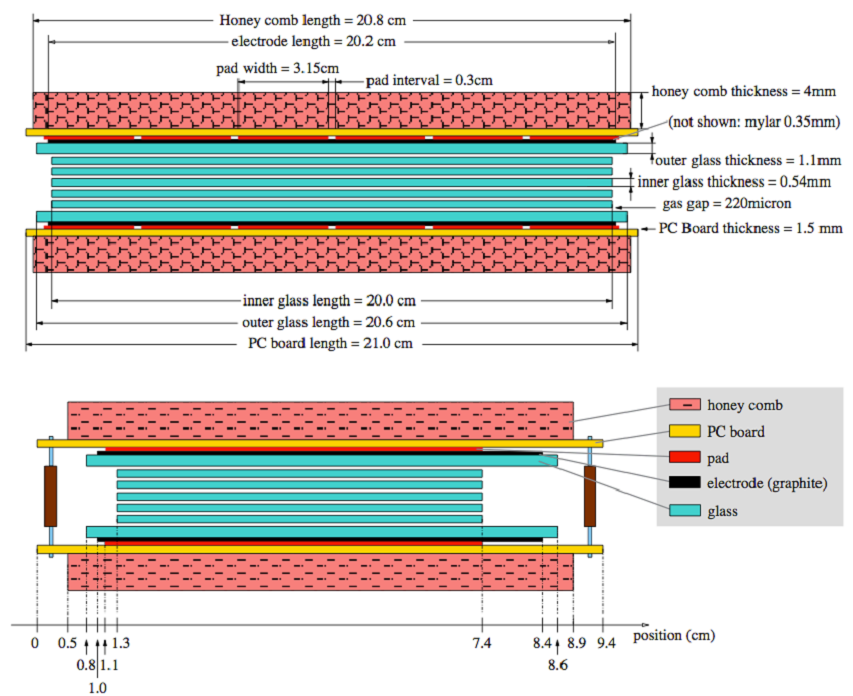
\includegraphics[keepaspectratio,width=0.8\textwidth]{rhic_star/TOFmrpc.png}
\figcaption{Two side views of MRPC~\cite{TOFdet}. The upper is for long side view and the lower is for short side view.}
 \label{tofmrpc}
\end{figure}

The whole TOF system consists of two parts, the barrel TOF and the VPD. The VPD has been explained in the former section. The VPD provided the ``start'' time of the charged particles while the barrel TOF provides the ``stop'' time. With HPTDC Integral Non-Linearity (INL) correction, T$_{0}$ correction (eliminating relative offsets caused by cable length and electronics), slewing correction (eliminating the time difference caused by different signal amplitude) applied (see details in~\cite{VPDdet,VPDTOFcalib0, VPDTOFcalib1}), the time resolutions of the VPD and barrel TOF can achieve $\sim$30 ps and $<$80 ps in heavy-ion collisions, respectively. With such time resolution, the TOF system significantly improves the particle identification capability. The $\pi/K$ separation momentum range is extended from $\sim$0.7 GeV/$c$ to $\sim$1.6 GeV/$c$ and $(\pi,K)/p$ separation from $\sim$1.1 GeV/$c$ to $\sim$3 GeV/$c$~\cite{tofpid}. Figure~\ref{tofbeta} shows the 1/$\beta$ distribution of different particle species measured by the TOF in U + U at $\sqrt{s_{NN}}$ = 193 GeV. For electron identification, the TOF is used to reject slow hadrons in cross-over $dE/dx$ regions which will be discussed in detail in Chapter~\ref{chap:analysis}. 

\begin{figure}[htbp]
\centering
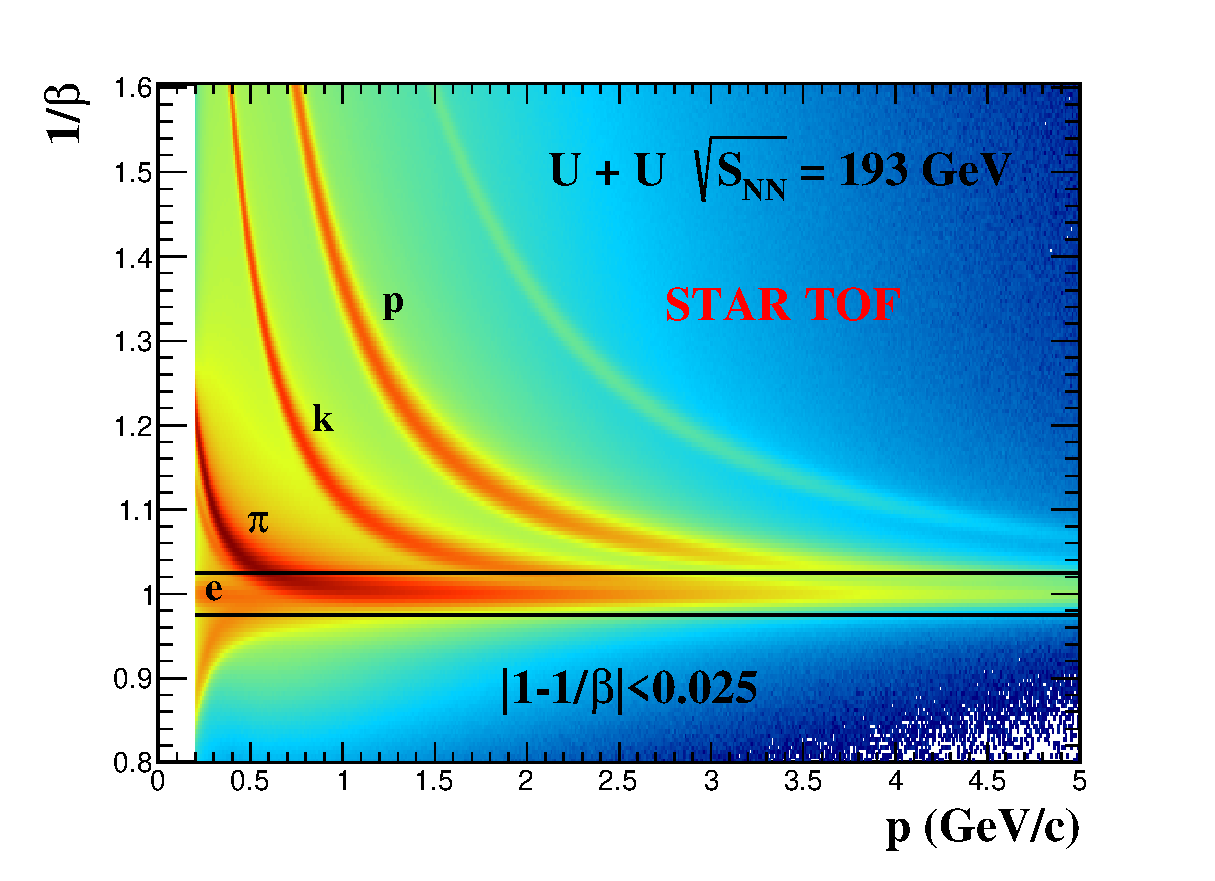
\includegraphics[keepaspectratio,width=0.8\textwidth]{rhic_star/betavsp.eps}
\figcaption{1/$\beta$ distribution for different particle species in U + U collisions at $\sqrt{s_{NN}}$ = 193 GeV.}
 \label{tofbeta}
\end{figure}

%封面是按照制本厂的要求制作的,其中行宽和行高都是固定的,中文标题最多占两行,英文标题最多占三行。如果您的题目超过了这个限制,请缩减题目长度,不要擅自修改模板中的相关配置参数。


  \chapter{Muon Telescope Detector}

A large-area, cost-effective Muon Telescope Detector (MTD) at mid-rapidity for the STAR can trigger on and identify muons based on its precise timing and modest position resolution, allowing us to measure dilepton through di-$\mu$ channel. Compared with electrons, muons have less background from gamma conversions and suffer less bremsstrahlung radiation energy loss effects in the detector materials. These make the muon be a more effective triggering particle in central nucleus-nucleus collisions at mid-rapidity at the STAR. The novel and compact device allows for the measurements of quarkonia, dilepton continuum (di-$\mu$ channel), as well as the correlation of heavy flavor quarks through their semi-leptonic decays (e-$\mu$ channel). The di-$\mu$ channel can be used to measure the J/$\psi$ meson over a broad transverse momentum range thanks to the low kinematic threshold of the MTD trigger on muons. It also has the potential to separate different $\varUpsilon$ states, predicted to melt at very different temperatures, as the bremsstrahlung radiation for muons is much smaller compared to electrons. The e-$\mu$ correlation can be used to distinguish between lepton pair production and heavy quark decays ($c + \overline{c} \rightarrow e + \mu(e), B \rightarrow e(\mu) + c \rightarrow e + \mu(e)$), allowing us directly access the QGP thermal radiation. The MTD will thus provide direct information on the temperature and the characteristics of color screening in the QGP created in RHIC collisions.

\section{MTD Configuration}

Out of the full MTD system, 10\%  (12 modules), 61\% (75 modules) and 100\% (122 modules) were installed in years 2012, 2013, 2014, respectively. The whole MTD system, covering $|\eta|$ < 0.5 and 2$\pi$ azimuthal, is mounted on BEMC PMT boxes behind the STAR magnet flux-return bars so called ``backlegs'' which serve as hadron absorbers. The schematic and physical picture are shown in Fig.~\ref{mtdsys}. There are 30 backlegs outside the magnetic coils to provide the return flux path for the magnetic field~\cite{STARmagnet} with only 28 of them mounted with MTD trays due to the mechanical constraints. Each backleg covers 8$^{\circ}$ in azimuthal while the gap between two backlegs covers 4$^{\circ}$. Nineteen of 28 MTD trays are five-module trays while two (BL8, BL24) of them are not fully shielded by the magnetic steels. Thus 3 $\times$ 5, 2 $\times$ 5 readout channels (exposed in the backleg gap) are disabled for BL8 and BL24, respectively, avoiding hot channels in the MTD trigger system. The remaining 9 bottom MTD trays are three-module trays due to the two cradles. Figure~\ref{mtdhitmap} shows the hit map of the MTD system during the run15 $p$ + $p$ at $\sqrt{s_{NN}}$ = 200 GeV.

\begin{figure}
\centering
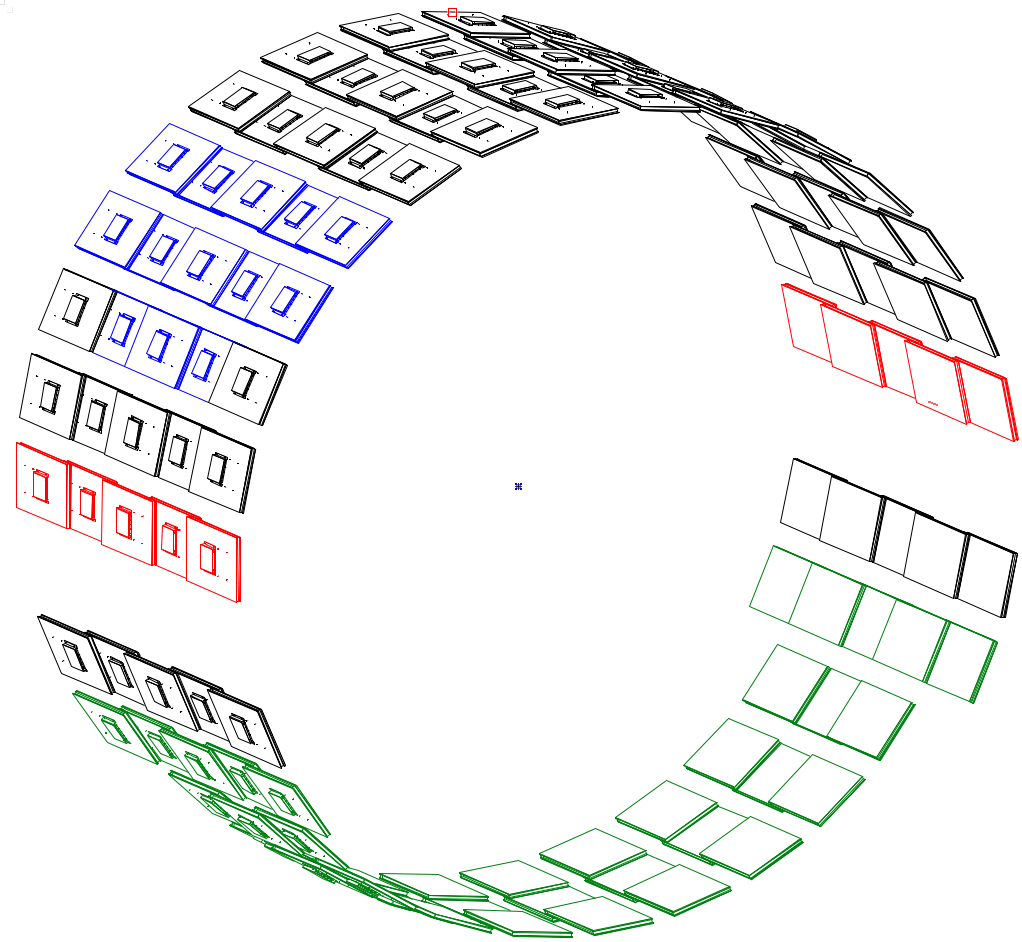
\includegraphics[width=0.48\textwidth]{mtd/MTD_schematics.png}
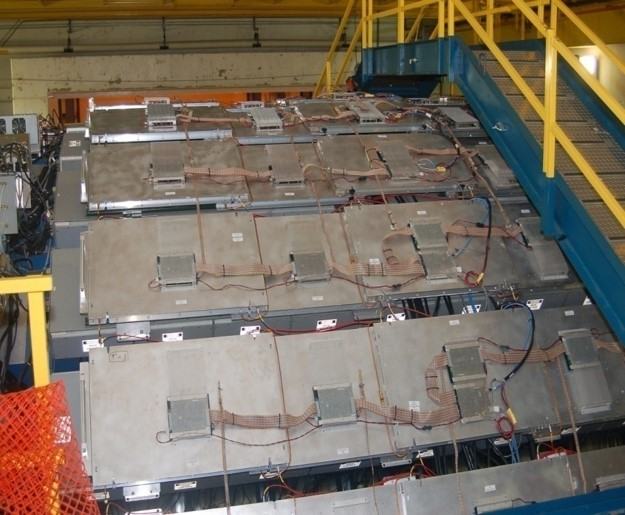
\includegraphics[width=0.48\textwidth]{mtd/MTD_reality.jpg}
\figcaption{(Left) The schematic view of the whole MTD system. Different colors represent the modules installed in different years: Blue - installed in year 2012; Black - installed in year 2013; Green and Red - installed in 2014, the two red trays are special trays with 2$\times$5 (in BL24) and 3$\times$5 (in BL8) readout channels disabled. (Right) The physical picture of the MTD system.}
\label{mtdsys}
\end{figure}

\begin{figure}[htbp]
\centering
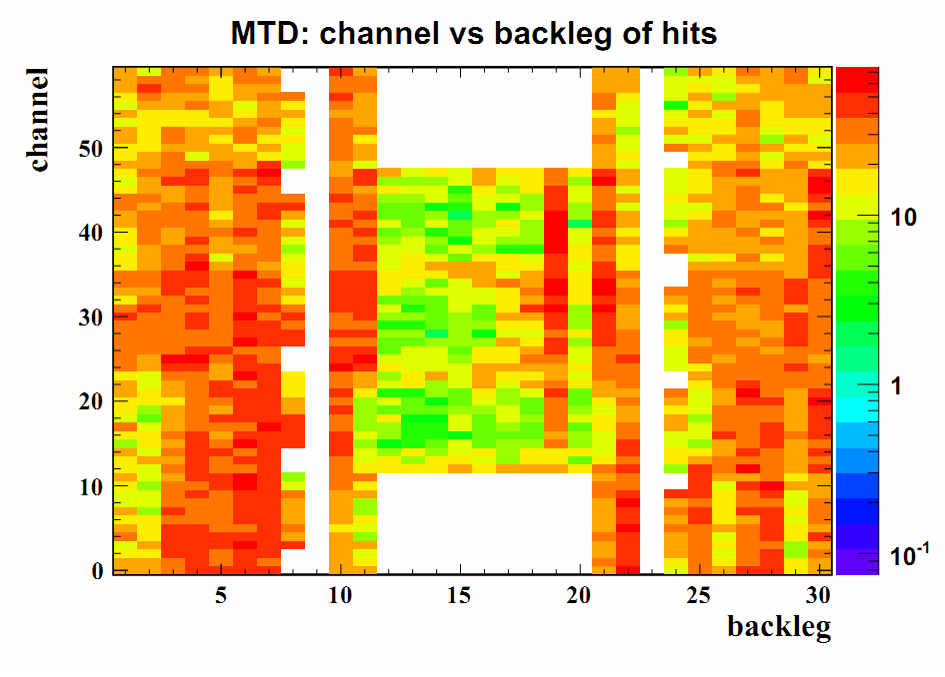
\includegraphics[keepaspectratio,width=0.7\textwidth]{mtd/MTDHitMap_pp200.png}
\vspace*{-5mm}
\figcaption{The hit map of the MTD system in the run15 $p$ + $p$ at $\sqrt{s_{NN}}$ = 200 GeV.}
 \label{mtdhitmap}
\end{figure}

The MTD detector is based on large Multi-gap Resistive Plate Chambers with long readout strips (LMRPC)~\cite{MTDdet}. Couple of prototypes with different designs were tested at T963 at Fermilab and beam line 3 at Institute of High Energy Physics (IHEP), resulting in $<$70 ps timing resolution and $\sim$1 cm spatial resolution along the readout strip with $>$95\% detection efficiency~\cite{MTDmrpc0,MTDmrpc1}. The final design of the LMRPC module is shown is Fig.~\ref{mtdmrpc}. The module has five 250 $\mu$m gas gaps which are defined by a stack of float glass sheets separated by a nylon monofilament fishing line. The thickness of the float glass (inner glass) sheets is 0.7 mm while the volume resistivity is $\sim$10$^{13}$ $\Omega\cdot$cm. The positive and the negative high voltage (HV) are applied to a coating of colloidal graphite paint (with surface resistivity of 1$\sim$10 M$\Omega$/$\Box$) on the external surface of the outer glass plates. The 3-D size of the outer glass is 890 $\times$ 559 $\times$ 1.1 mm$^{3}$. The total area of each LMRPC module defined by the Printed Circuit Board (PCB) is 915 $\times$ 580 mm$^{2}$ while the active area defined by the inner glass sheets is 874 $\times$ 543 mm$^{2}$. Twelve double-end readout strips are fixed on the PCB facing inner glasses, and the size of each strip is 870 mm long and 38 mm wide. The width of the intervals between two readout strips is 6 mm. Two pieces of 10 mm thick honeycomb-board are attached to the outer surfaces of the detector to reduce structural deformations.

\begin{figure}[htbp]
\centering
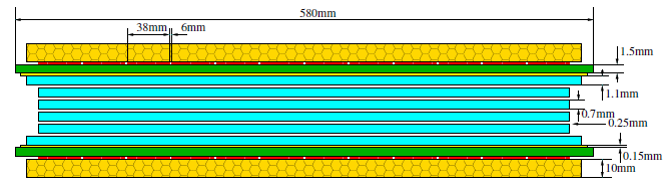
\includegraphics[keepaspectratio,width=1\textwidth]{mtd/MTDmrpc.png}
\figcaption{A schematic side-view of the LMRPC module.}
 \label{mtdmrpc}
\end{figure}

\begin{figure}[htbp]
\centering
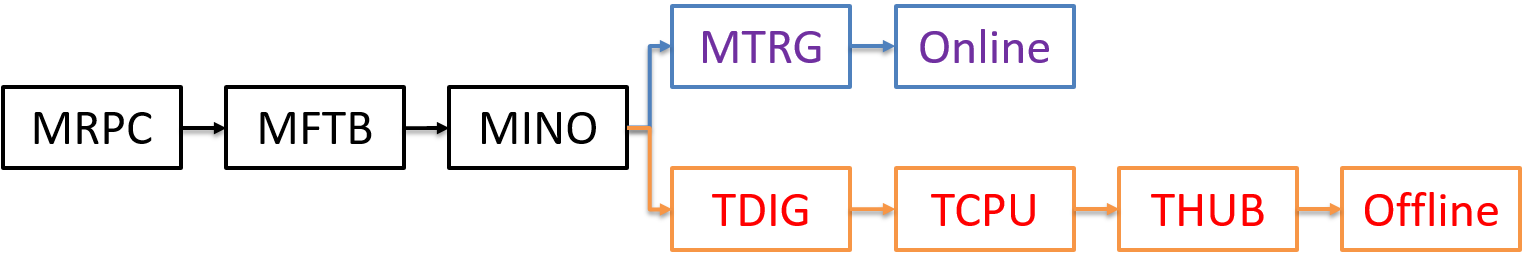
\includegraphics[keepaspectratio,width=1\textwidth]{mtd/MTDelectronics.png}
\figcaption{A schematic view of the MTD electronics and readout paths.}
 \label{mtdelectronics}
\end{figure}

The signals from the LMRPC modules are digitized by two different sets of electronics, shown in Fig.~\ref{mtdelectronics}, while the electronics for precise timing measurements is the same as that for the STAR TOF~\cite{TOFelectronics}. The signals from the MTD are sent to a MINO board to perform a leading-edge discrimination through a MFTB board. The outputs of the MINO board are sent to a TDIG board which uses the CERN HPTDC chip~\cite{HPTDC} to digitize the arrival times of the signals with respect to an externally input free-running 40 MHz clock. Each TDIG board uses three HPTDC chips in ``high resolution'' mode. The digitized times are 21 bit data words with a dynamic range of 52 $\mu$s and the least significant bit (LSB) time conversion is 25 ns/1024 $\approx$24.4 ps. The magnitude of the MTD signals is characterized by the width of output digital signals from MINO board called ``Time Over Threshold'' (TOT). A copy of  MINO outputs is passed to a MTRG board through a MTRG cable and combined with a logical "OR". Then, the outputs of the MTRG board are sent to electronics in the STAR trigger system called ``QT boards'' through long coax cables. The QT board performs magnitude and timing measurements using an analog-to-digital (ADC) and timing-to-amplitude (TAC) circuitry. The ADC and TAC measurements are each 12-bit numbers while the TAC timing measurement uses a common stop with respect to the 9.4 MHz RHIC clock with a digital-to-time conversion of $\sim$18 ps/LSB. The trigger logic of the MTD system will be discussed in details in Sec.~\ref{mtdtriggersection}. 

\section{MTD Trigger Logic}
\label{mtdtriggersection}

The whole MTD system (122 MTD modules) is divided into 28 MTD trigger patches. In general, one trigger patch is composed of 5 MTD modules in the same $\eta$ region. The same $\eta$ guarantees that the path lengths from collision vertex to the MTD modules of the same trigger patch are the same. Due to the asymmetric MTD geometry in $\phi$ direction, there are some trigger patches composed of less than 5 MTD modules. The signals from the MTD trigger patches are sent to QT boards (first layer of trigger system) numbered MT001 - MT004. The detail trigger patch compositions and the logic from trigger patches to QT boards can be found in Fig.~\ref{mtdtrgflow} and App.~\ref{chap:mtdtrgmap}. A timing cut is applied in the QT board to reject the noise. For each QT board, two earliest hit signals (with largest TAC sum - the read-out strips of MTD module are double-ended) are selected and sent to the next layer of the trigger system (MT101). Then all eight signals in MT101 are compared to the VPD time, and an online timing window is applied to reject the background and slow hadrons. The results of the selection are sent to the third layer of the trigger system called TF201, resulting in a 8-bit sequence. At last, the MTD related bits are formed in the Trigger Control Unit (TCU) based on the 8-bit sequence in TF201. The MTD related triggers generated by combining the bits from the MTD and other detectors (VPD, ZDC etc.), trigger on the interested collision events. The trigger flow of the MTD system for Run14 and Run15 is shown in Fig.~\ref{mtdtrgflow}. 

\begin{figure}[htbp]
\centering
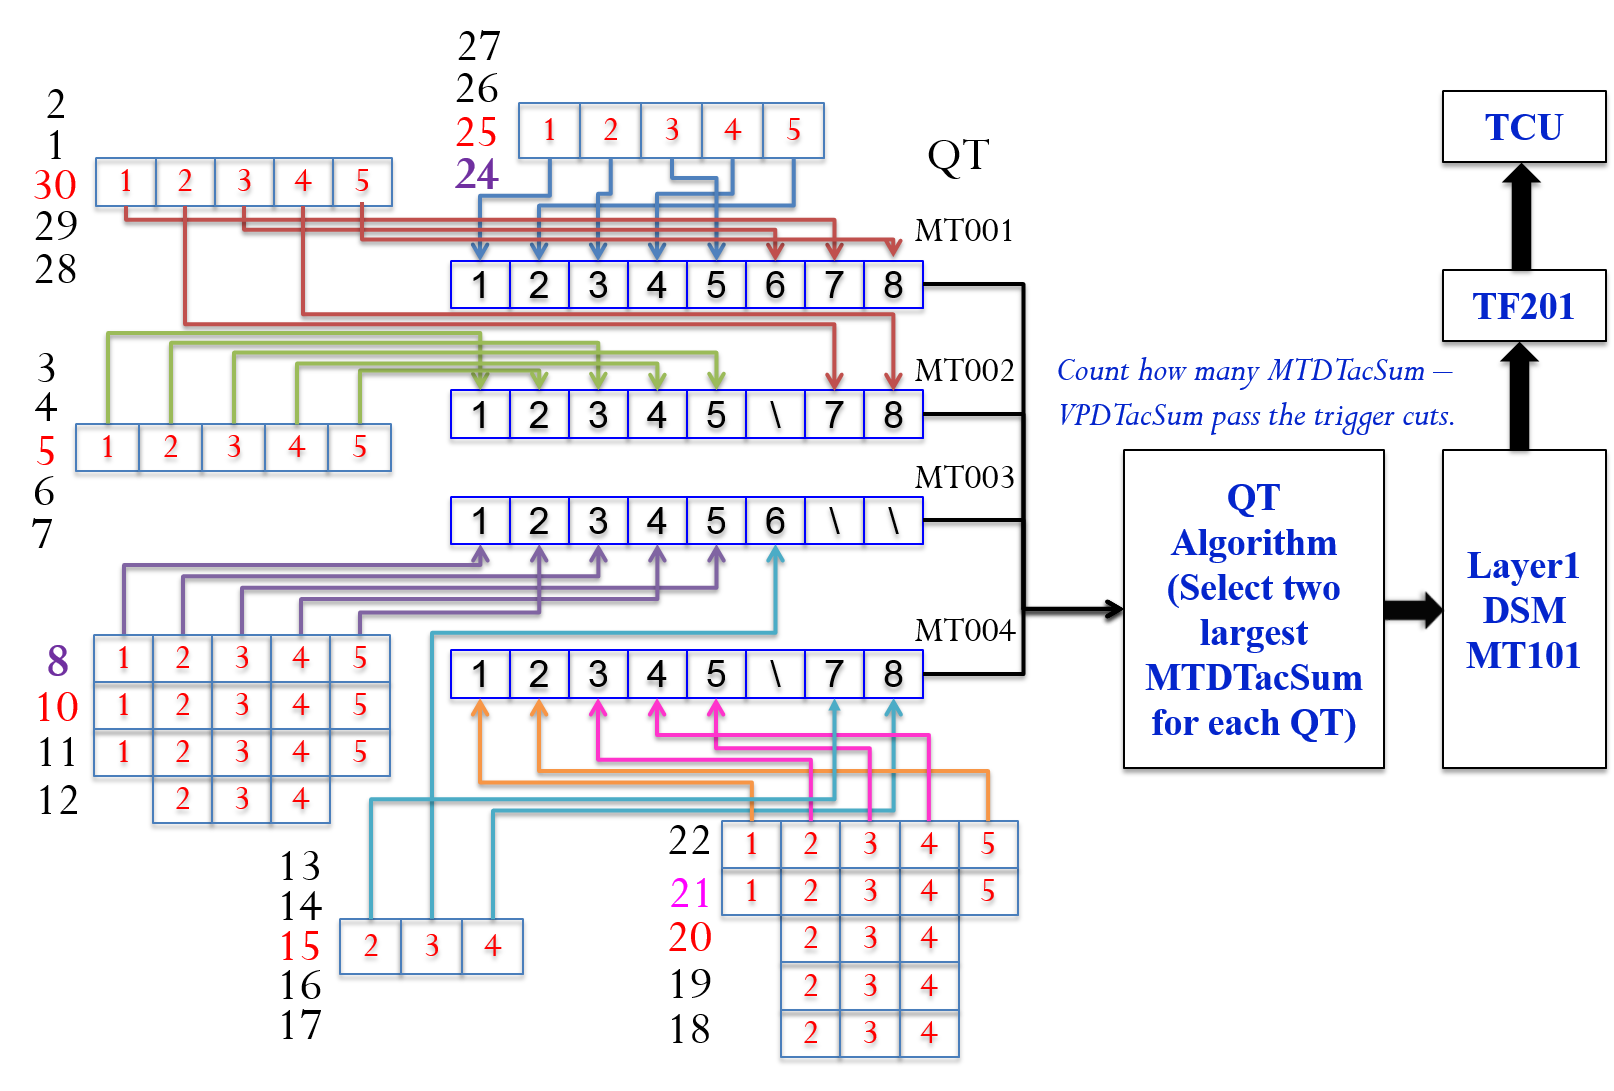
\includegraphics[keepaspectratio,width=1\textwidth]{mtd/mtd_trigger_flow.png}
\figcaption{The trigger flow of the MTD system in Run14 and Run15. In general, one trigger patch consists of 5 MTD modules (e.g. BL28-1, BL29-1, BL30-1, BL1-1, and BL2-1 form a trigger patch). Due to the asymmetric MTD geometry, there are some trigger patches consist of $<$ 5 MTD modules (e.g BL21-1 and BL22-1 form a trigger patch). The \textcolor{red}{\textbf{red}} backleg IDs represent that these backlegs are mounted with MTRG boards. Beside these backlegs, Module 1 and 5 of  BL21 (\textcolor{magenta}{\textbf{magenta}}) are also mounted with MTRG boards. BL8 and BL24 (\textcolor{violet}{\textbf{violet}}) are two special backlegs with 3 $\times$ 5 and 2 $\times$ 5 readout strips disabled, respectively.}
 \label{mtdtrgflow}
\end{figure}

\subsection{QT Algorithm}
The QT algorithm outputs two largest TAC pair sums (two earliest signal pairs from two trigger patches) with an 2-bit ID for each TAC pair sum. The 2-bit ID can tell which TPC sectors are covered by the corresponding trigger patch for partial tracking or ``DAQ 10K'' purpose. ``DAQ 10K'' is a sparse readout scheme for the TPC that would enable STAR to acquire events at rates of 10 kHz for classes of physics where only few TPC sectors contain all the necessary particle information. Each QT board has 32 inputs in a line and the inputs can be numbered 1 - 32 from top to bottom. Each MTD trigger patch has an East-end and West-end readout (mark East-end as $J2$, West-end as $J3$ for the modules located in positions 1, 2, and 3; mark West-end as $J2$, East-end as $J3$ for the modules located in positions 4 and 5) while each end readout occupies two QT input channels recording the magnitude and timing information.

In the QT board, an alignment is applied to each TAC channel, at the very beginning, to eliminate the differences of flight time from collision vertex to MTD tirgger patches due to different path lengths and electronics, shown in Fig.~\ref{tacalignment}. Second, a slewing correction is applied to each TAC channel based on the value of the corresponding ADC channel. After the TAC value modification, the TAC value is filtered by ``Good Hit'' criteria which requires the TAC value for a channel is greater than ``TAC\_Min'' and less than ``TAC\_Max'', to reject noise hits. Both of the $J2$ and $J3$ TAC values from the same trigger patch must satisfy the ``Good Hit'' requirement, otherwise, the TAC sum (TAC$_{sum}$ = TAC$_{J2}$ + TAC$_{J3}$) is set to 0 for this trigger patch. And then, the hit position correction for each trigger patch is applied according to the TAC difference between East-end and West-end TAC (TAC$_{J2}$ - TAC$_{J3}$) to eliminate the influence of different path lengths caused by different hit positions in the same trigger patch along $z$ direction (along beam axis), especially for the outermost trigger patches. The 13-bit corrected TAC pair sum is then truncated to 10 bits. Bits [3:12] (starting from zero) are kept. The two largest truncated, corrected TAC pair sums together with the corresponding 2-bit IDs are then found and transfered to the next layer of the trigger system (MT101).

\begin{figure}
\centering
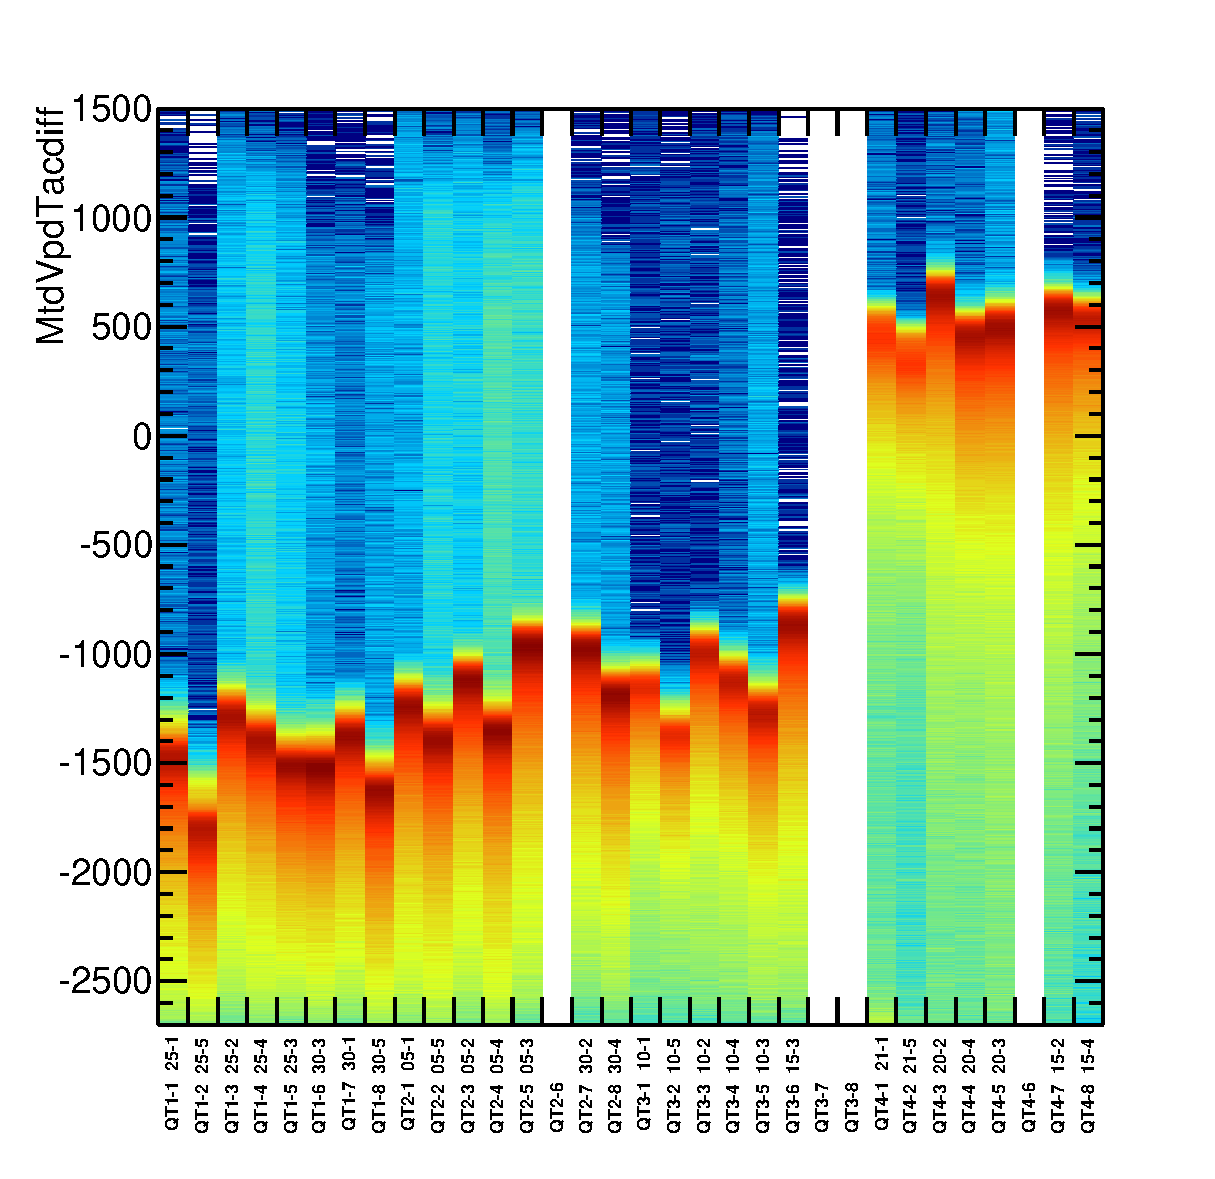
\includegraphics[width=0.48\textwidth]{mtd/MtdVpdTacdiffRawvsQtChannel.eps}
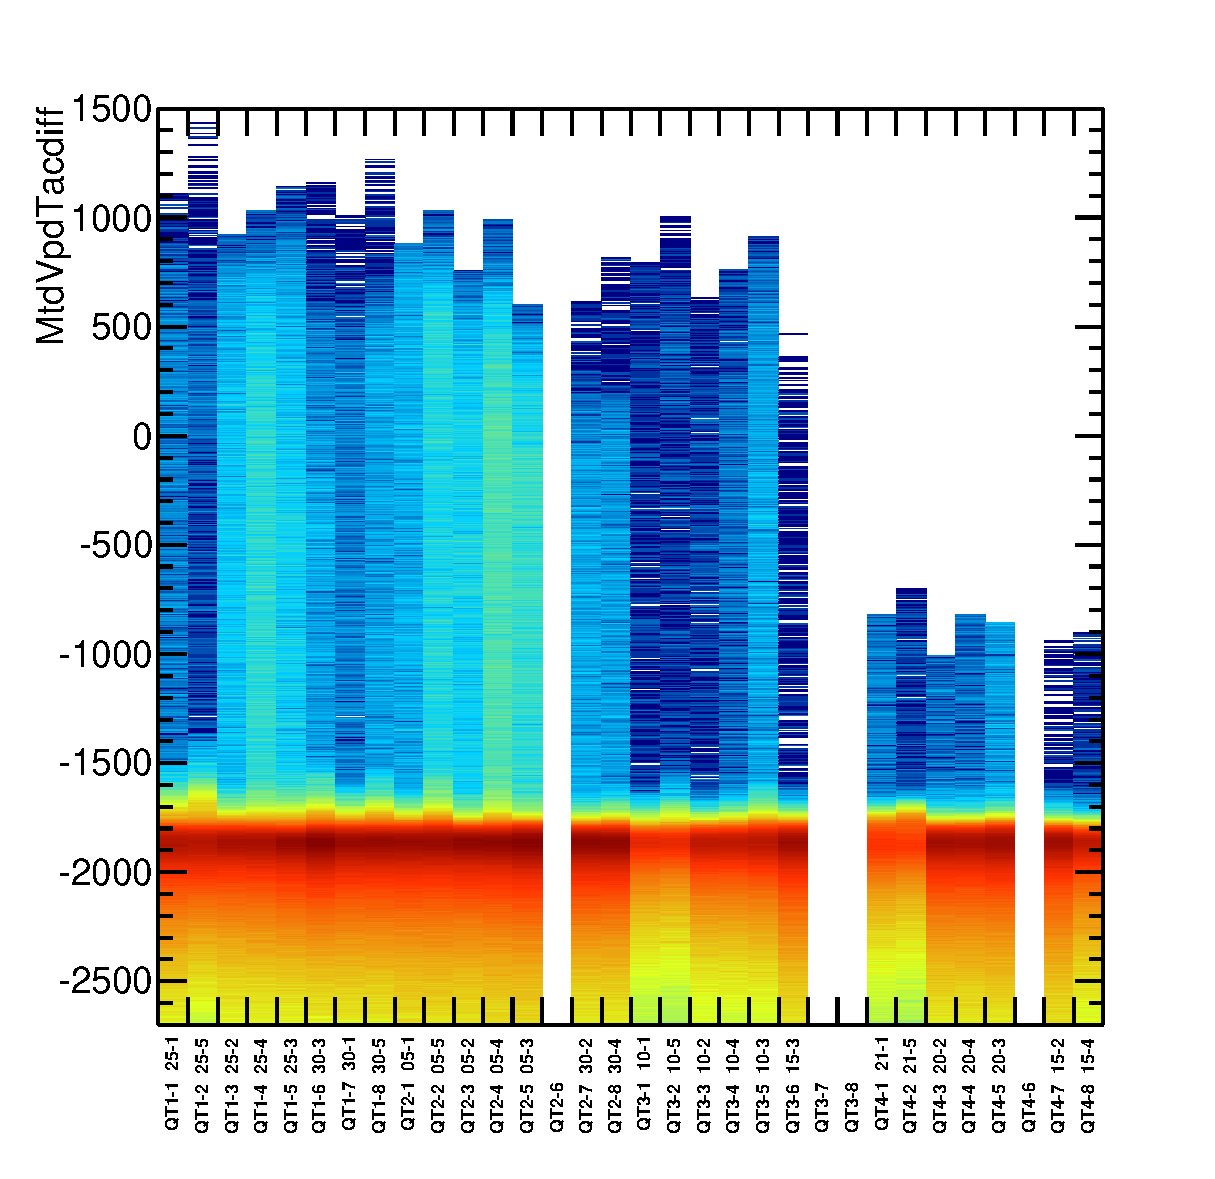
\includegraphics[width=0.48\textwidth]{mtd/MtdVpdTacdiffCorvsQtChannel.eps}
\figcaption{(Left) ``MTD TAC sum - VPD TAC sum'' vs. trigger patch before the TAC alignment in Run 14 Au + Au at $\sqrt{s_{NN}}$ = 200 GeV. (Right) ``MTD TAC sum - VPD TAC sum'' vs. trigger patch after the TAC alignment in Run 14 Au + Au at $\sqrt{s_{NN}}$ = 200 GeV.}
\label{tacalignment}
\end{figure}

\subsection{DSM Algorithm (MT101$\rightarrow$TF201$\rightarrow$TCU)}
The MT101 DSM receives its data through a TDSMI, so there are 10 12-bit input channels. The algorithm receives the 2 best TAC sums from each of the 4 MTD QT boards, and the IDs of those sums. It also receives the fastest (largest) TAC values from the QT boards covering the East and West sides of the VPD. The VPD TAC sum is calculated and truncated from 13 bits to 10 bits. Bits [3:12] (starting from zero) are kept. Then the algorithm finds the difference between the MTD and VPD TAC sums. All 8 MTD VPD TAC differences (MTD\_TAC\_Sum - VPD\_TAC\_Sum + 1024, to guarantee the MTD VPD TAC difference is larger than zero) are checked to determine if they are inside a timing window. If either TAC from East side of VPD, or TAC from West side of VPD, or MTD TAC sum is $\leq$0, the corresponding MTD VPD TAC difference is directly set to zero. Those that are inside the window are counted, and the count is sent to TF201. Meanwhile a 8-bit sequence (``MTD-VPD TAC difference in window'' bits) is sent to TF201 for indicating that each MTD VPD TAC difference is inside the timing window or not (``1'' is inside the window, ``0'' is outside the window). The MTD VPD TAC differences are also sorted to find the two largest values that are inside the window. The 2-bit IDs of those two channels are sent on to MT201 for the DAQ10k readout scheme. In addition, a bit is set if at least two of the incoming MTD TAC sums is non-zero. That bit is sent to TF201 for use as a debugging and monitoring trigger, or for triggering on cosmic rays. The MTD related bits in TCU is formed based on the information stored in TF201. Di-muon bit is set to TRUE if the count of MTD VPD TAC difference inside the timing window is $\geq$2, otherwise set to FALSE. Single-muon bit is set to TRUE if the count is $\geq$1 while MTD-Cosmic bit is set to TRUE if at least two of the MT101 incoming MTD TAC sums are non-zero. The MTD related triggers (di-muon, single-muon, e-muon, mtd-cosmic-ray) are formed based on the combination of TCU bits from the MTD detector and other relevant detectors. Table~\ref{mtdsampledlum} shows luminosity and statistics sampled by the MTD detector in physics Run13, Run14 and Run15. The MTD muon trigger efficiency for the Run14 Au + Au at $\sqrt{s_{NN}}$ = 200 GeV (Centrality: 0-60\%) is shown in Fig.~\ref{muontrgeff}. The overall muon trigger efficiency caused by trigger electronics and algorithm is around 78\%.

\begin{table}[htp]
\centering
\caption{The luminosity and statistics sampled by the MTD related triggers. ``single-muon'' trigger has at least one online muon candidate (provided by the MTD and VPD) and 5 cm online vertex cut (provided by the VPD). ``di-muon'' trigger has at least two online muon candidates and no online vertex cut. ``di-muon-5-hft'' trigger has at least two online muon candidates, 5 cm online vertex cut and read out HFT information. ``di-muon-30-hft'' trigger has at least two online muon candidates, 30 cm online vertex cut and read out HFT information. ``e-muon'' trigger has at least one online muon candidate, one online electron candidate (provided by the BEMC) and 30 cm online vertex cut.}
\label{mtdsampledlum}
\newcolumntype{V}{!{\vrule width 1.6pt}}
\begin{tabular}{Vc|c|c|r@{.}l|r@{.}lV}
\Xhline{1.6pt}
\textbf{Year} & \textbf{Collision Species} & \textbf{Trigger Type} & \multicolumn{2}{c|}{\textbf{Statistics}} & \multicolumn{2}{cV}{\textbf{Luminosity}} \\

\Xhline{1.2pt}
\multirow{3}{*}{\thead{\textbf{2013}\\\textbf{(Run13)}}} & \multirow{3}{*}{$p$ + $p$ @ 500 GeV} & single-muon & 21&1 M & 0&07 pb$^{-1}$ \\ \cline{3-7}
 && di-muon & 118&5 M & 28&27 pb$^{-1}$ \\ \cline{3-7}
 && e-muon & 52&1 M & 18&16 pb$^{-1}$ \\ 
 
 \Xhline{1.2pt}
 \multirow{8}{*}{\thead{\textbf{2014}\\\textbf{(Run14)}}} & \multirow{5}{*}{Au + Au @ 200 GeV} & single-muon & 317&4 M & 0&28 nb$^{-1}$ \\ \cline{3-7}
 && di-muon & 2635&0 M & 14&17 nb$^{-1}$ \\ \cline{3-7}
 && di-muon-5-hft & 110&7 M & 0&40 nb$^{-1}$ \\ \cline{3-7}
 && di-muon-30-hft & 79&6 M & 0&27 nb$^{-1}$ \\ \cline{3-7}
 && e-muon & 256&2 M & 2&57 nb$^{-1}$ \\ \cline{2-7}
& \multirow{3}{*}{He$^{3}$ + Au @ 200 GeV} & single-muon & 18&8 M & 0&45 nb$^{-1}$ \\ \cline{3-7}
&& di-muon & 96&6 M & 45&63 nb$^{-1}$ \\ \cline{3-7}
&& e-muon & 28&2 M & 8&48 nb$^{-1}$ \\ 

 \Xhline{1.2pt}
 \multirow{9}{*}{\thead{\textbf{2015}\\\textbf{(Run15)}}} & \multirow{3}{*}{$p$ + $p$ @ 200 GeV} & single-muon & 74&1 M & 0&48 pb$^{-1}$ \\ \cline{3-7}
 && di-muon & 320&4 M & 122&13 pb$^{-1}$ \\ \cline{3-7}
 && e-muon & 102&6 M & 45&92 pb$^{-1}$ \\ \cline{2-7}
& \multirow{3}{*}{$p$ + Au @ 200 GeV} & single-muon & 14&8 M & 0&74 nb$^{-1}$ \\ \cline{3-7}
&& di-muon & 266&2 M & 409&97 nb$^{-1}$ \\ \cline{3-7}
&& e-muon & 53&5 M & 60&62 nb$^{-1}$ \\ \cline{2-7}
& \multirow{3}{*}{$p$ + Al @ 200 GeV} & single-muon & 4&4 M & 1&07 nb$^{-1}$ \\ \cline{3-7}
&& di-muon & 93&5 M & 1035&44 nb$^{-1}$ \\ \cline{3-7}
&& e-muon & 4&2 M & 42&17 nb$^{-1}$ \\

\Xhline{1.6pt}
\end{tabular}
\end{table}

\begin{figure}[htbp]
\begin{minipage}[htbp]{0.50\linewidth}
\centering
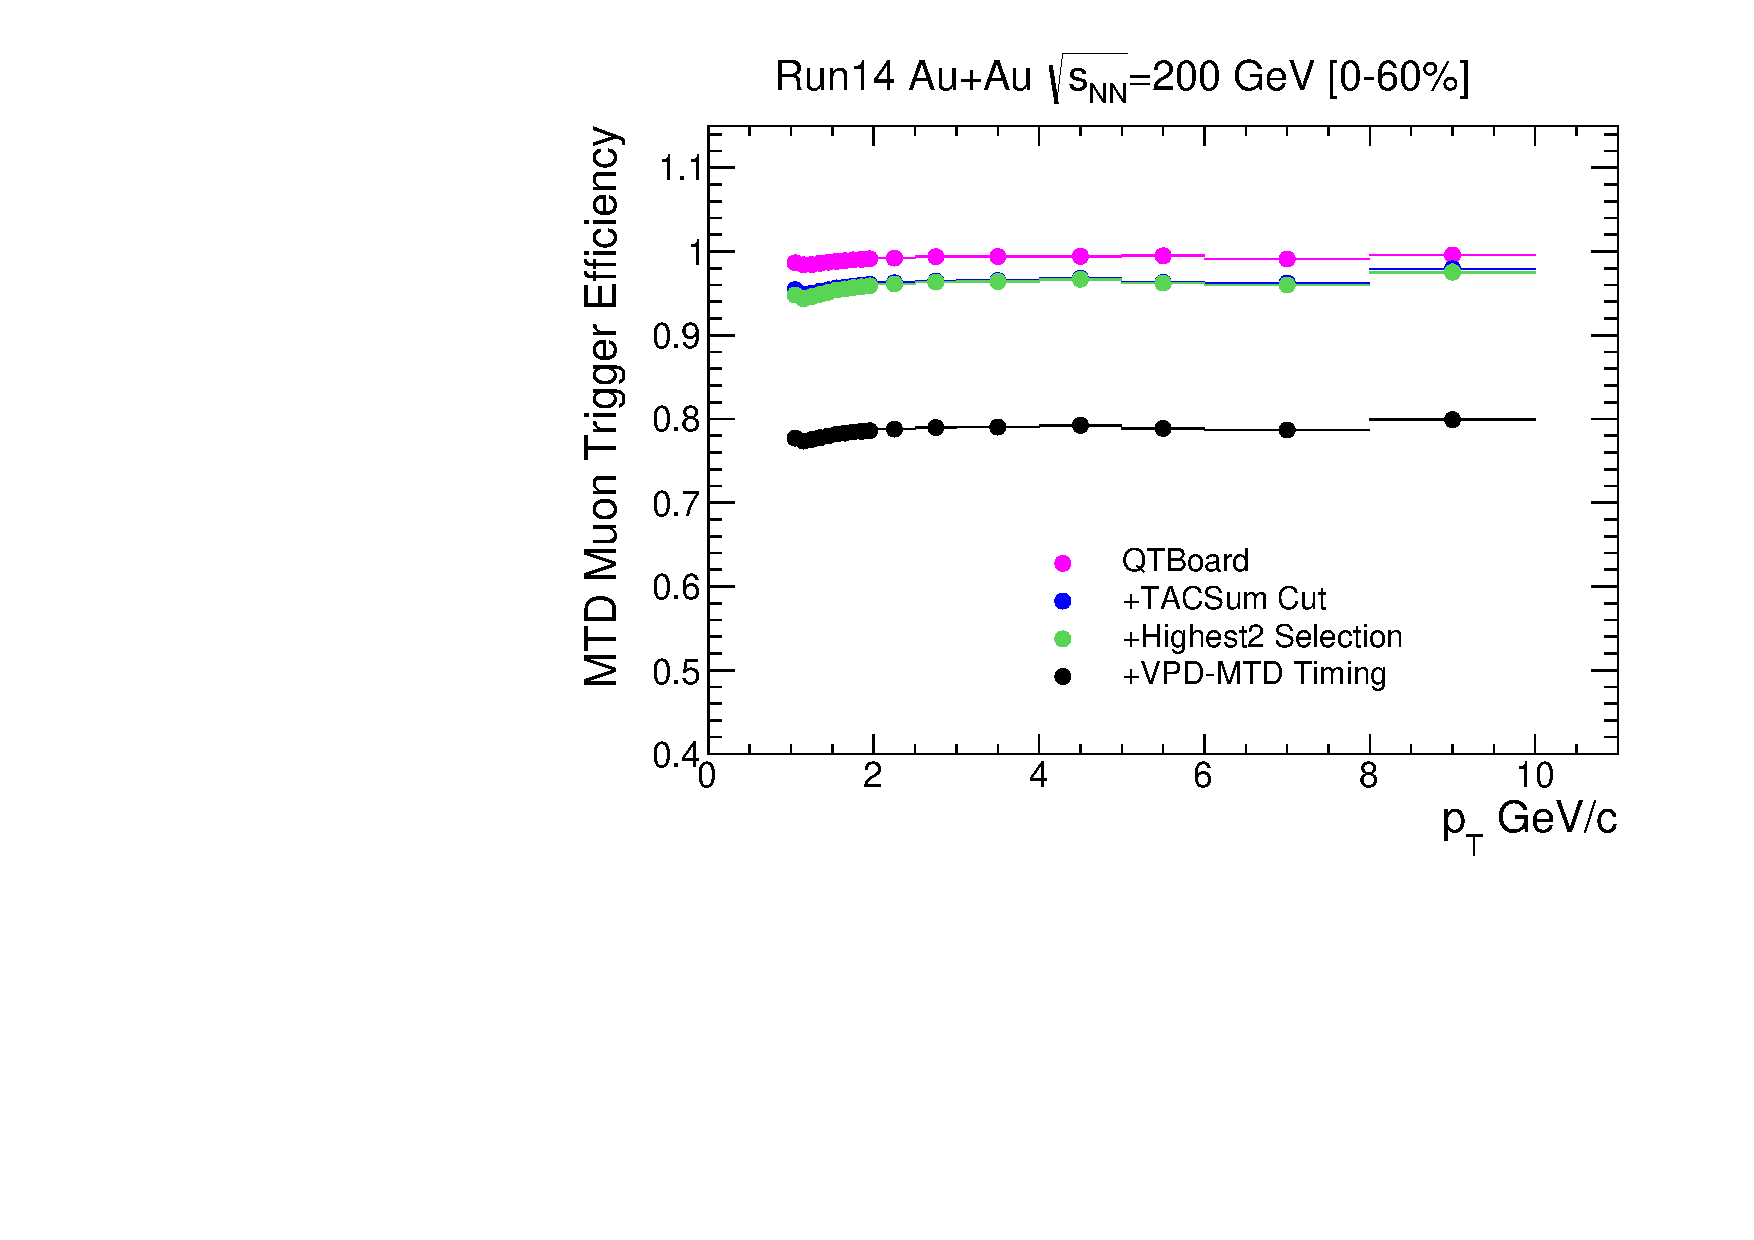
\includegraphics[angle=-90,width=1.0\textwidth]{mtd/MTDTriggerEfficiency.pdf}
\caption{The MTD muon trigger efficiency as a function of $p_{T}$ for the Run14 Au + Au at $\sqrt{s_{NN}}$ = 200 GeV (Centrality: 0-60\%). The muon trigger efficiency including the contribution of both trigger electronics and algorithm is around 78\%.\label{muontrgeff}}
\end{minipage}
\hfill
\begin{minipage}[htbp]{0.48\linewidth}
\centering
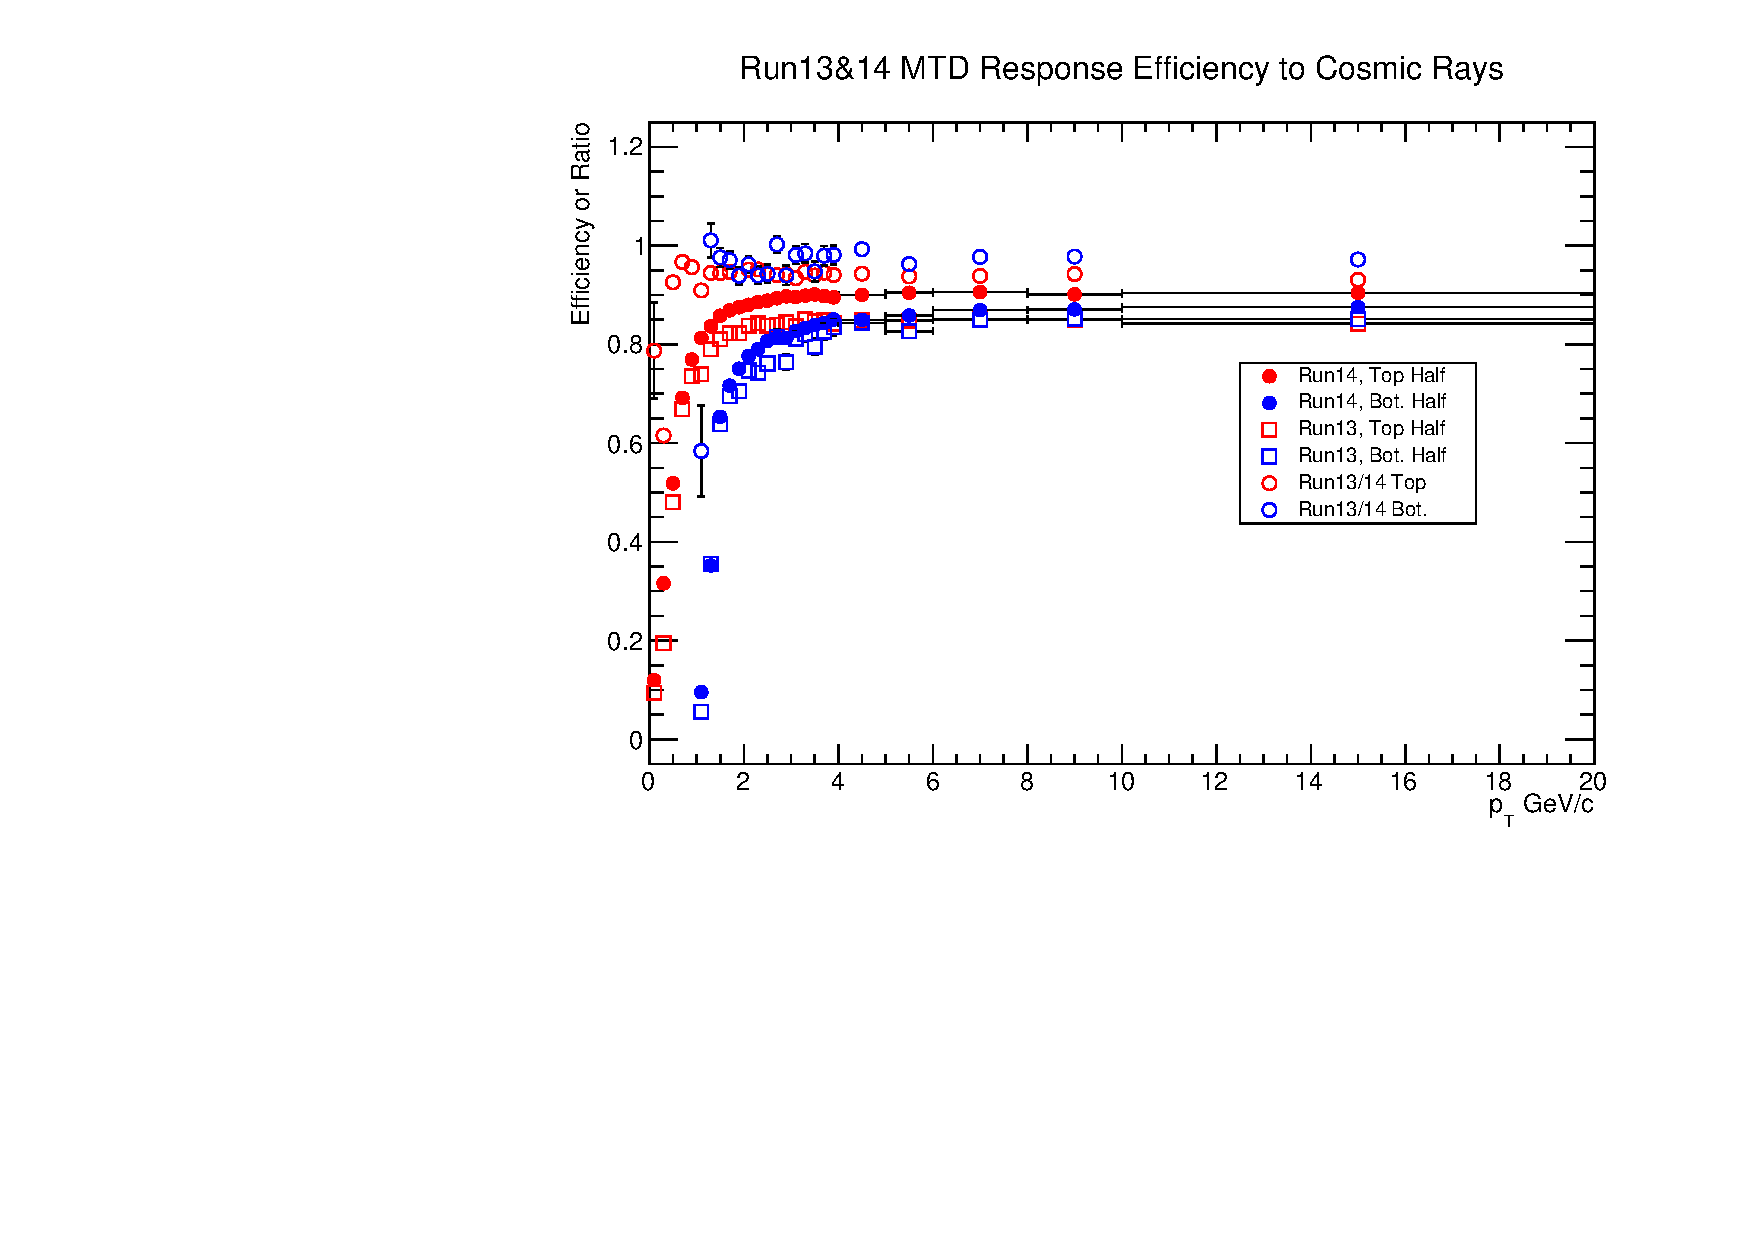
\includegraphics[angle=-90,width=1.0\textwidth]{mtd/MTDResponseEff.pdf} 
\caption{The MTD response efficiency as a function of muon $p_{T}$ for Run13 and Run14. The dots are Run14 response efficiency. The open squares are Run13 response efficiency. The circles are the response ratio between Run13 and Run14.\label{mtdresponseeff}}
\end{minipage}
\end{figure}

\begin{figure}[htbp]
\centering
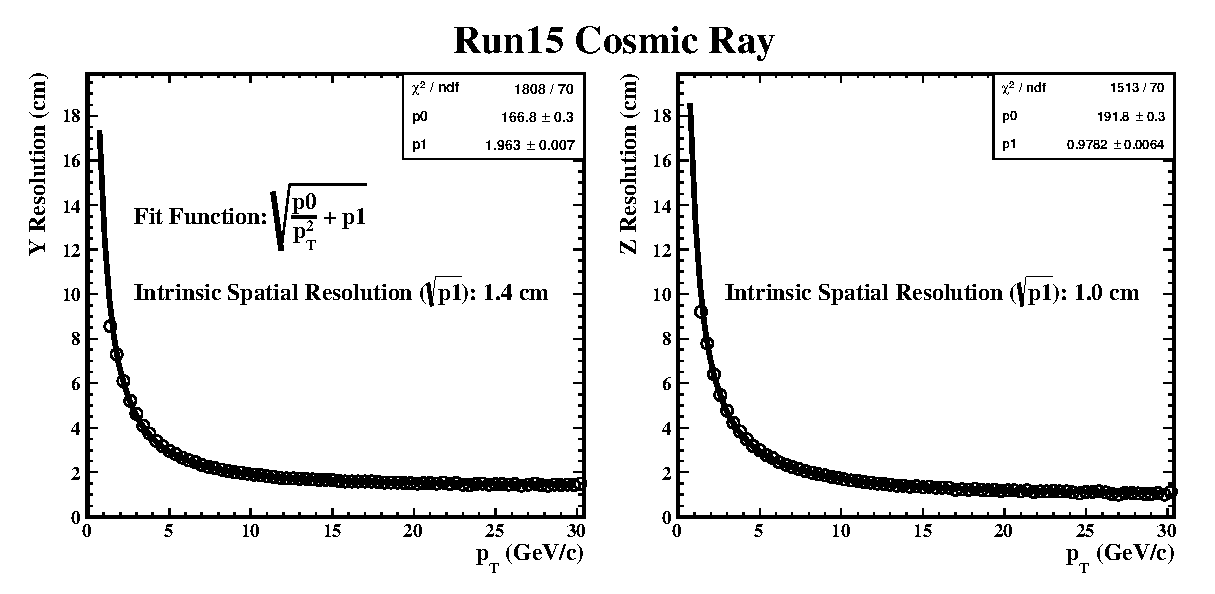
\includegraphics[keepaspectratio,width=1\textwidth]{mtd/posRes.eps}
\figcaption{The intrinsic spatial resolutions of the MTD along $y$ (left panel) and $z$ (right panel) direction as a function of $p_{T}$.}
 \label{posres}
\end{figure}

\begin{figure}[htbp]
\centering
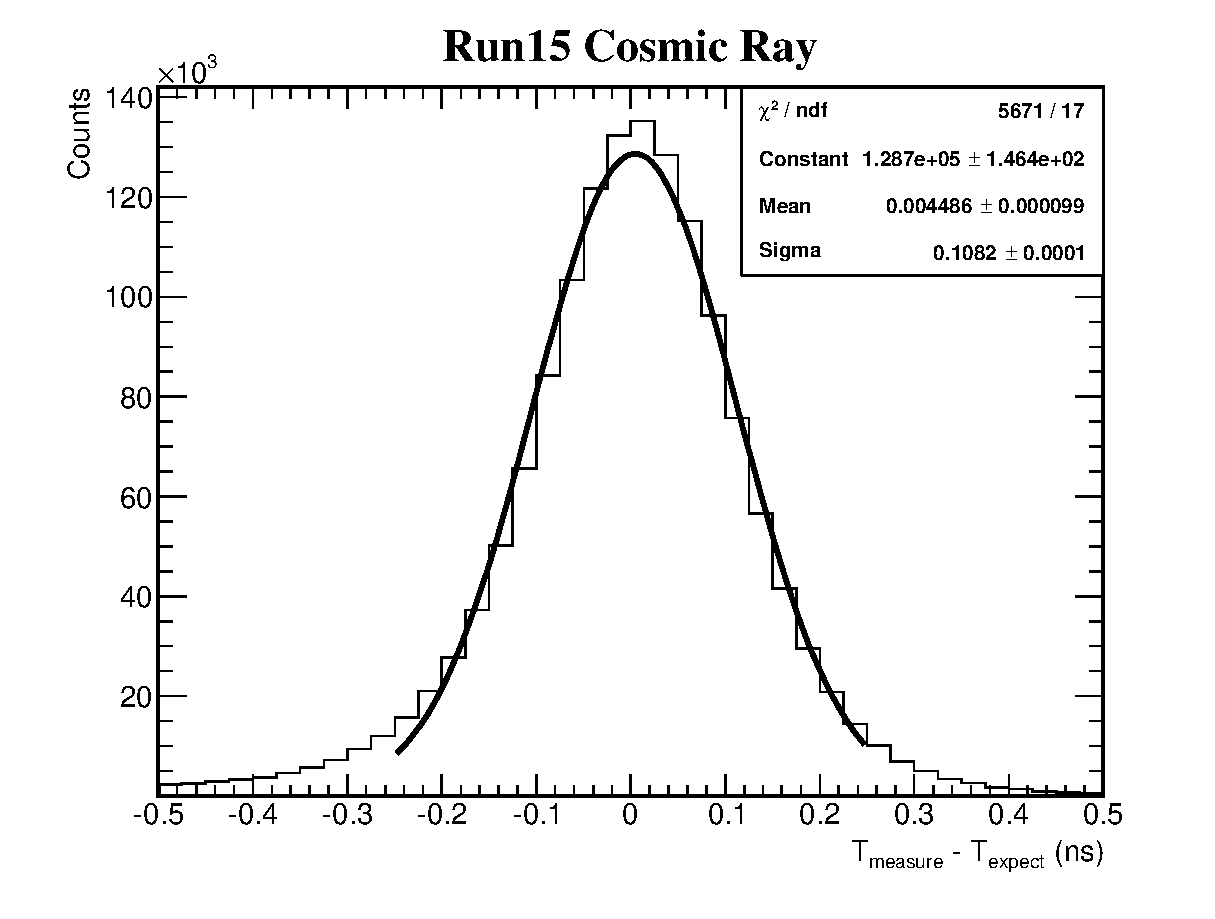
\includegraphics[keepaspectratio,width=0.6\textwidth]{mtd/timeRes.eps}
\figcaption{The overall time resolutions of the MTD (including the starting time contribution, provided by the TOF) after T$_{0}$ and slewing correction.}
 \label{timeRes}
\end{figure}

\section{MTD Performance and Physics Results}
The performance of the MTD system is studied through cosmic ray muons which allow to calibrate the detectors and measure their response efficiency, timing, and spatial resolution due to their very small multiple scattering effect in the detector material. The MTD response efficiency, including both of intrinsic and readout electronics response, can be obtained through calculating the ratio between tracks matched with MTD and tracks projected to MTD. Figure~\ref{mtdresponseeff} shows the MTD response efficiency for Run13 and Run14. The response efficiency trends as a function of $p_{T}$ for Run13 and Run14 are similar. The MTD response efficiency of Run13 is $\sim$85\% for both top half and bottom half while that of Run14 is $\sim$90\%, $\sim$85\% for top half and bottom half, respectively. The top half MTD response efficiency of Run13 is lower than that of Run14, due to electronics damage caused by an unexpected beam loss named ``blue abort kicker prefire''. The $p_{T}$ shift of the MTD response efficiency curves between top half and bottom half is because the cosmic ray muons pass through the magnetic steel firstly and lose energy before they are measured by the TPC. Thus $p_{T}$ measured by the TPC is smaller than the real $p_{T}$ in top half. The spatial resolution, in the $z$ direction (along the readout strips or beam axis direction) and the azimuthal direction ($\phi$ direction, perpendicular to the strips, also called $y$ direction with respect to the MTD module) , of the MTD is measured using the distance between the measured hit position and the track extrapolated position. Figure~\ref{posres} shows the dependence of the spatial resolution along the $y$ direction (left panel, $\Delta$y = R$\times$$\Delta\phi$) and $z$ direction (right panel) as a function of the muon transverse momentum. These data were fit with a function ($\sqrt{(p0/p_{T}^{2}) + p1}$) driven by the expectation for the contribution to the measured resolutions from multiple scattering in the detector materials. The intrinsic spatial resolution is then given by $\sqrt{p1}$. According to Fig.~\ref{posres}, the intrinsic spatial resolutions of the MTD along $y$ and $z$ direction are 1.4 and 1.0 cm, respectively. The time resolution of the MTD system can be measured via the time difference between the measured flight time from the TOF to the MTD and expected time using track extrapolation. After T$_{0}$ and slewing correction, an overall time resolution of 108 ps can be achieved, as shown in Fig.~\ref{timeRes}. The whole procedure and details are described in~\cite{MTDcalib}. The overall time resolution shown in Fig.~\ref{timeRes} includes the contributions from the starting time (56 - 65 ps, $\sigma_{TOF}$/$\sqrt{2}$) and the multiple scattering ($\sim$25 ps for 6 GeV/$c$ muons). The muon can be thus identified in the heavy-ion collisions via precise timing and modest position information.


\begin{figure}[htbp]
\begin{minipage}[htbp]{0.48\linewidth}
\centering
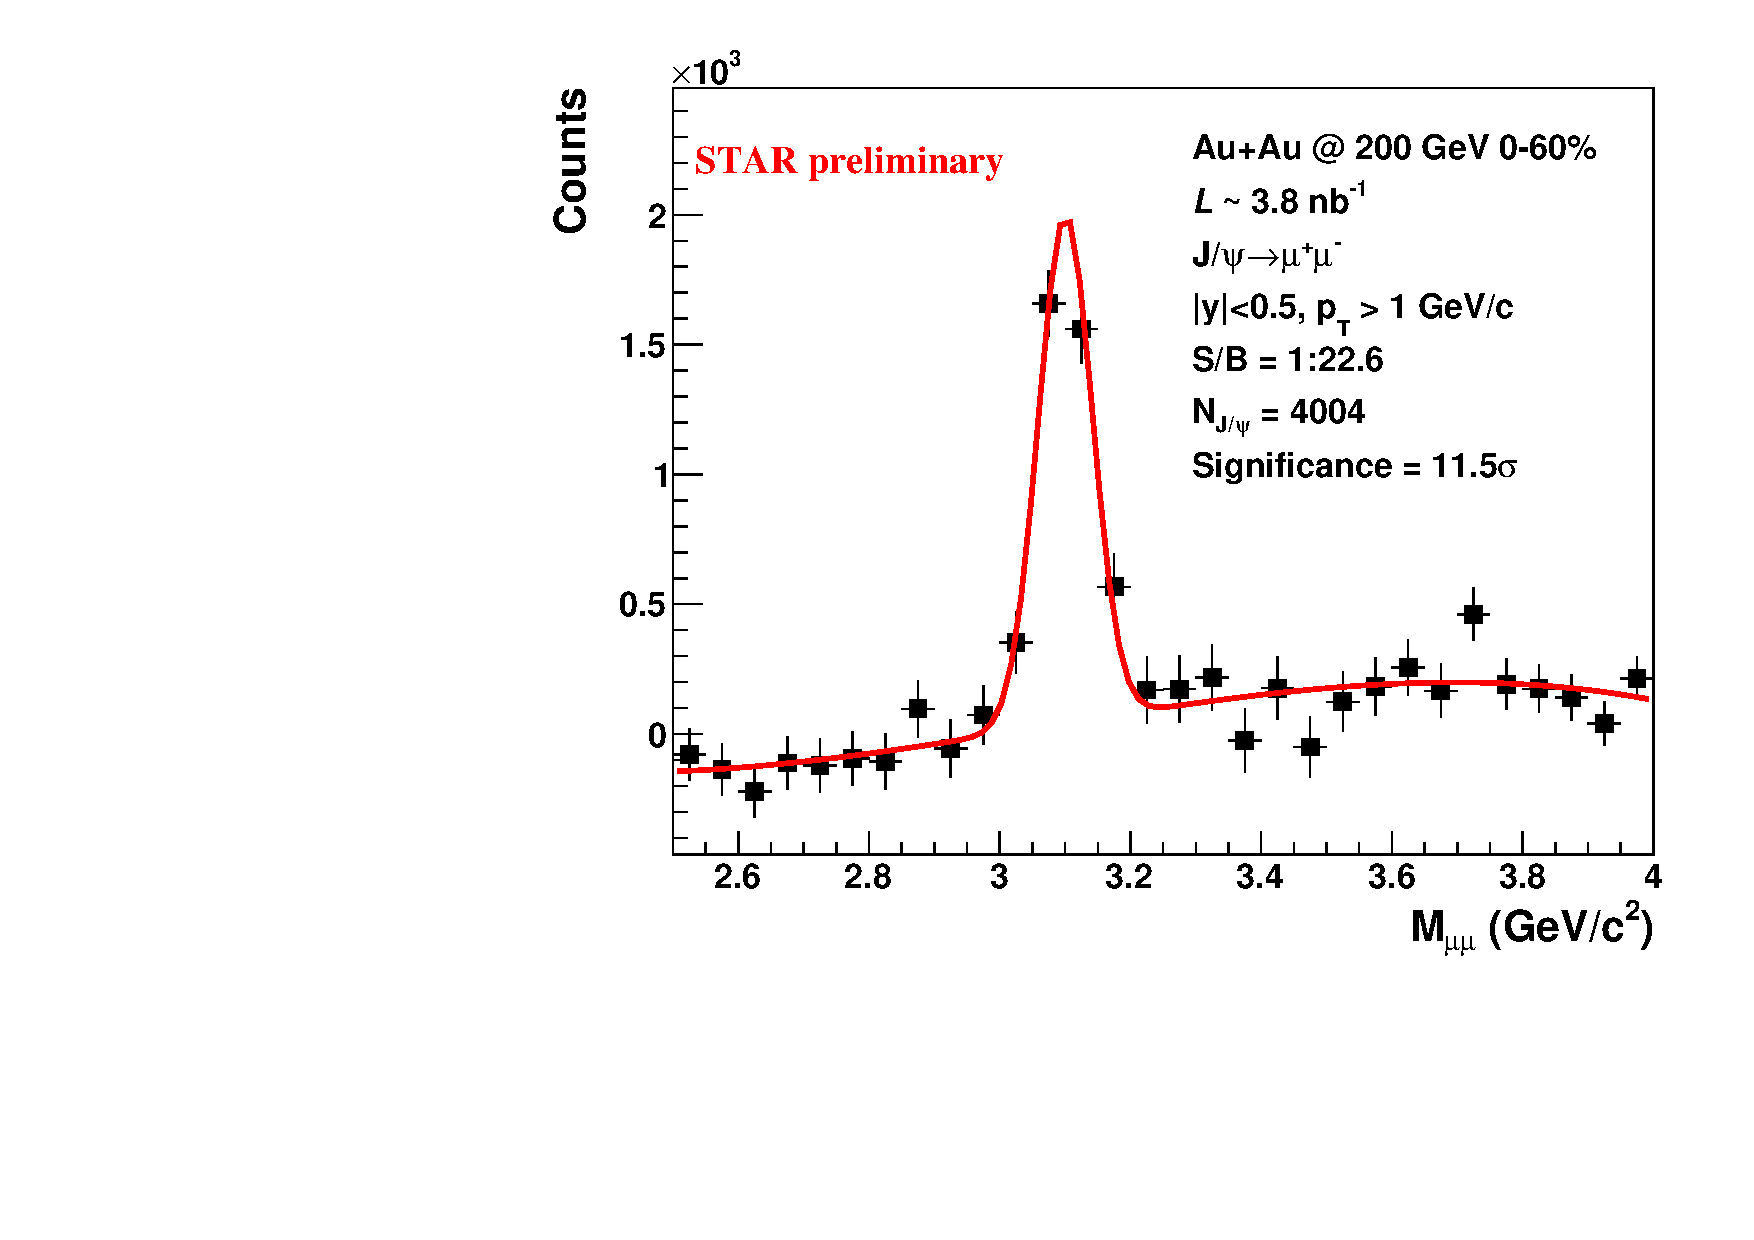
\includegraphics[angle=-90,width=1.0\textwidth]{mtd/Run14_JpsiInvMass.pdf}
\caption{Invariant mass distribution of unlike-sign muon pairs after subtracting mixed-event background. A Gaussian + Pol3 fit to the distribution is shown as the red line.\label{jpsiviamumu}}
\end{minipage}
\hfill
\begin{minipage}[htbp]{0.48\linewidth}
\centering
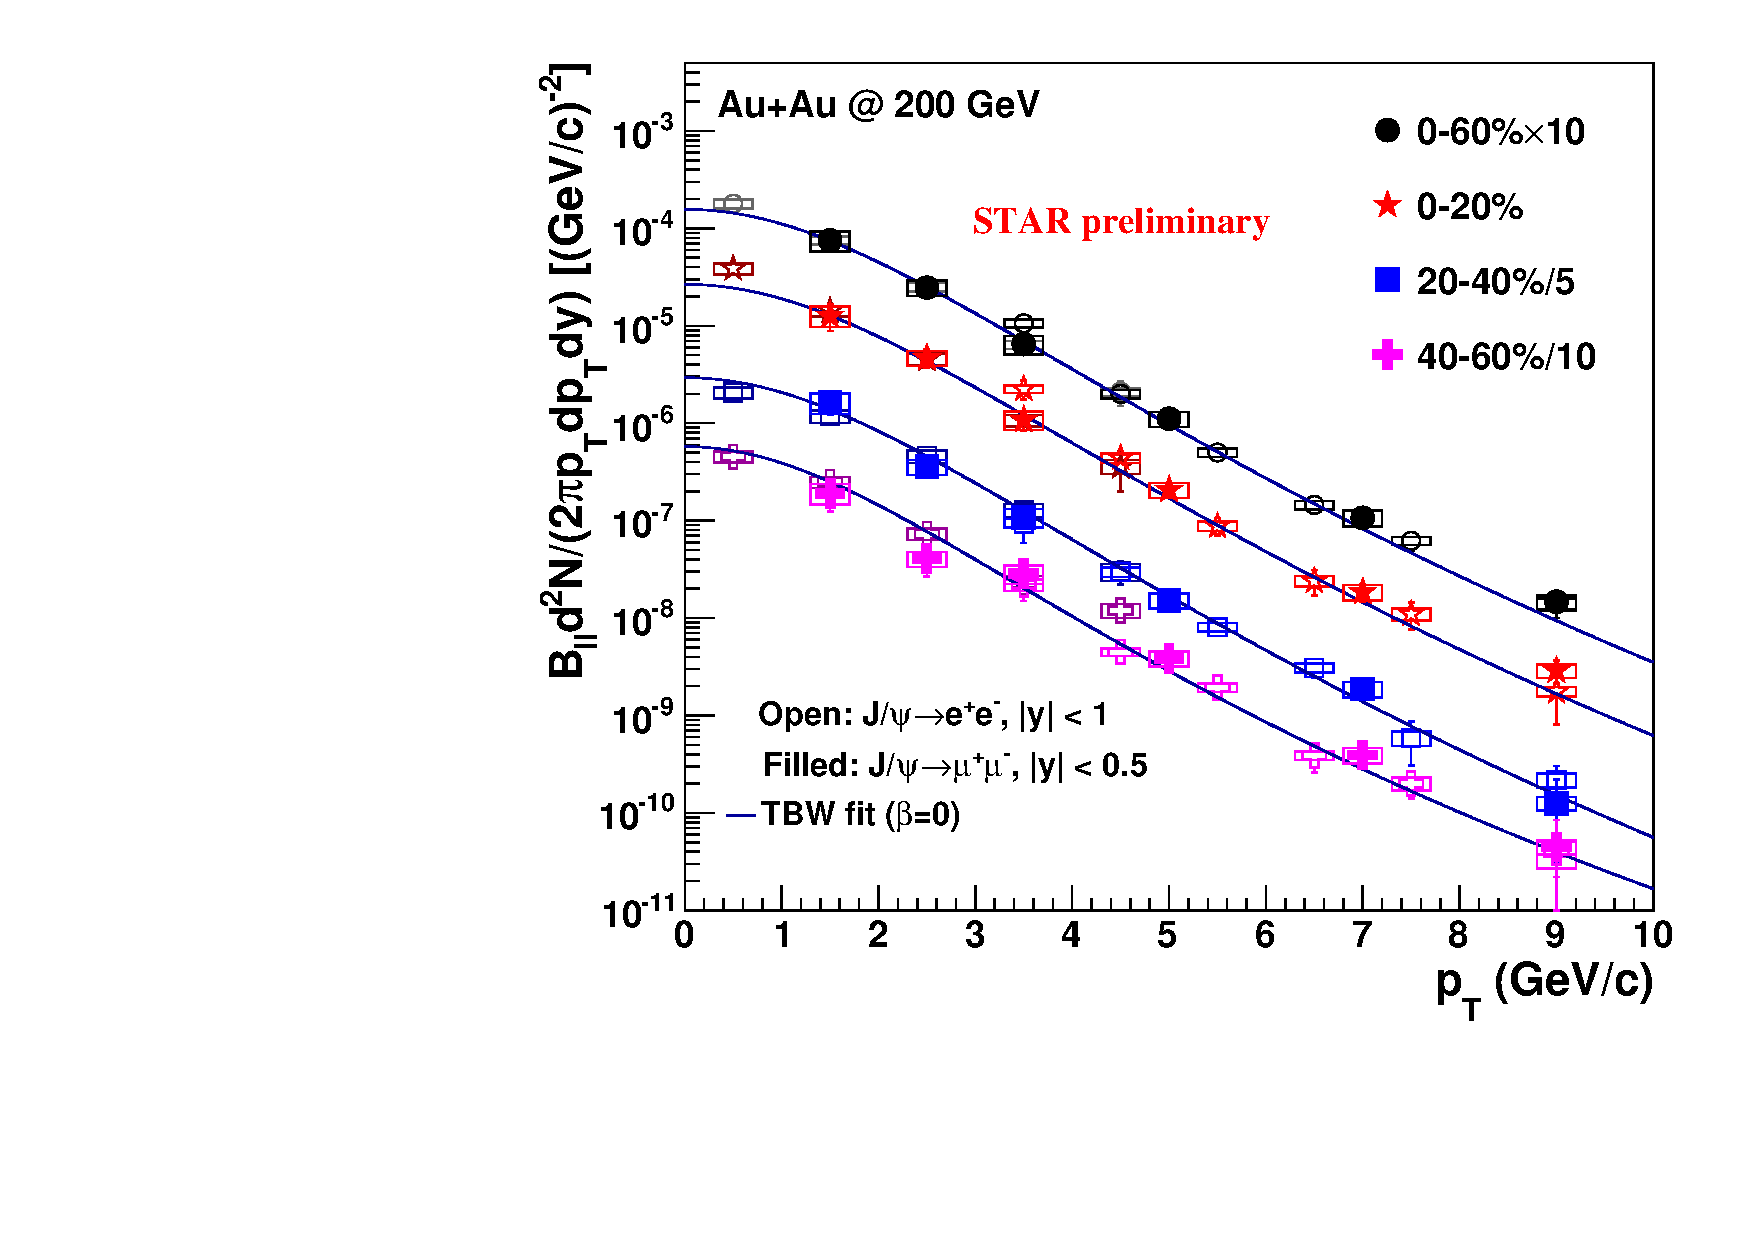
\includegraphics[angle=-90,width=1.0\textwidth]{mtd/Run14_JpsiInvYield_vs_pub.pdf} 
\caption{Invariant yield of inclusive J/$\psi$ vs. $p_{T}$ in four centralities bins (solid markers), with comparison to the published di-electron results (open markers)~\cite{JpsiViaee0, JpsiViaee1}. The solid lines are Tsallis Blast-wave fits to the di-electron results.\label{jpsiyield}}
\end{minipage}
\end{figure}

Lots of physics results from the MTD for Run13 $p$ + $p$ at $\sqrt{s_{NN}}$ = 500 GeV and Run14 Au + Au at $\sqrt{s_{NN}}$ = 200 GeV already came out~\cite{MTDResultpp500, MTDResultAuAu200}. Only part of them are briefly mentioned here. The invariant mass distribution of unlike-sign muon pairs after subtracting the combinatorial background is shown in Fig.~\ref{jpsiviamumu} for Run14 Au + Au at $\sqrt{s_{NN}}$ = 200 GeV. The combinatorial background is estimated via mixed-event technique, namely pairing muons from different events with similar properties. A clear J/$\psi$ peak can be seen with a total of about 4k J/$\psi$ candidates using only $\sim$26.7\% statistics collected in Run14 200 GeV Au + Au collisions. The distribution is fitted by a Gaussian distribution plus a third-order polynomial function (accounting for the residual background). The raw J/$\psi$ is then extracted after subtracting residual background within the mass range of 2.9 - 3.3 GeV/$c^{2}$. After the efficiency losses and detector acceptance are corrected for, the invariant $p_{T}$ spectra of inclusive J/$\psi$ are shown in Fig.~\ref{jpsiyield} for four centrality bins, compared with the published results via di-electron channel~\cite{JpsiViaee0, JpsiViaee1}. The invariant yield spectra measured by di-muon and di-electron channels agree well. $\varUpsilon$ mesons are also reconstructed via the di-muon channel as shown in Fig.~\ref{upsilonviamumu}, where the combinatorial and correlated background are subtracted by using the like-sign same event technique, namely pairing the same charge sign muons into pairs in the same event. A combined fit, constraining the line shape of different $\varUpsilon$ states determined by embedded simulated signals into real data and the shape of residual background ($b\overline{b}$ + Drell-Yan) estimated through PYTHIA simulation, is used to extract the total $\varUpsilon$ yield and the ratio of ($\varUpsilon_{2S}$ + $\varUpsilon_{3S}$)/($\varUpsilon_{1S}$). A total of 50 $\pm$ 22 $\varUpsilon$s are observed and a factor of 6 more statistics is expected combining the rest of 2014 data and the data that will be taken in 2016. Figure~\ref{upsilonproj} shows the projection for the statistical uncertainty on the ratio of ($\varUpsilon_{2S}$ + $\varUpsilon_{3S}$)/($\varUpsilon_{1S}$) using the full statistics of Run14 and Run16 for Au + Au at $\sqrt{s_{NN}}$ = 200 GeV, together with the published results in different collision systems at different energies~\cite{UpsilonWorldwide, UpsilonSTAR, UpsilonCMS}.

\begin{figure}[htbp]
\begin{minipage}[htbp]{0.48\linewidth}
\centering
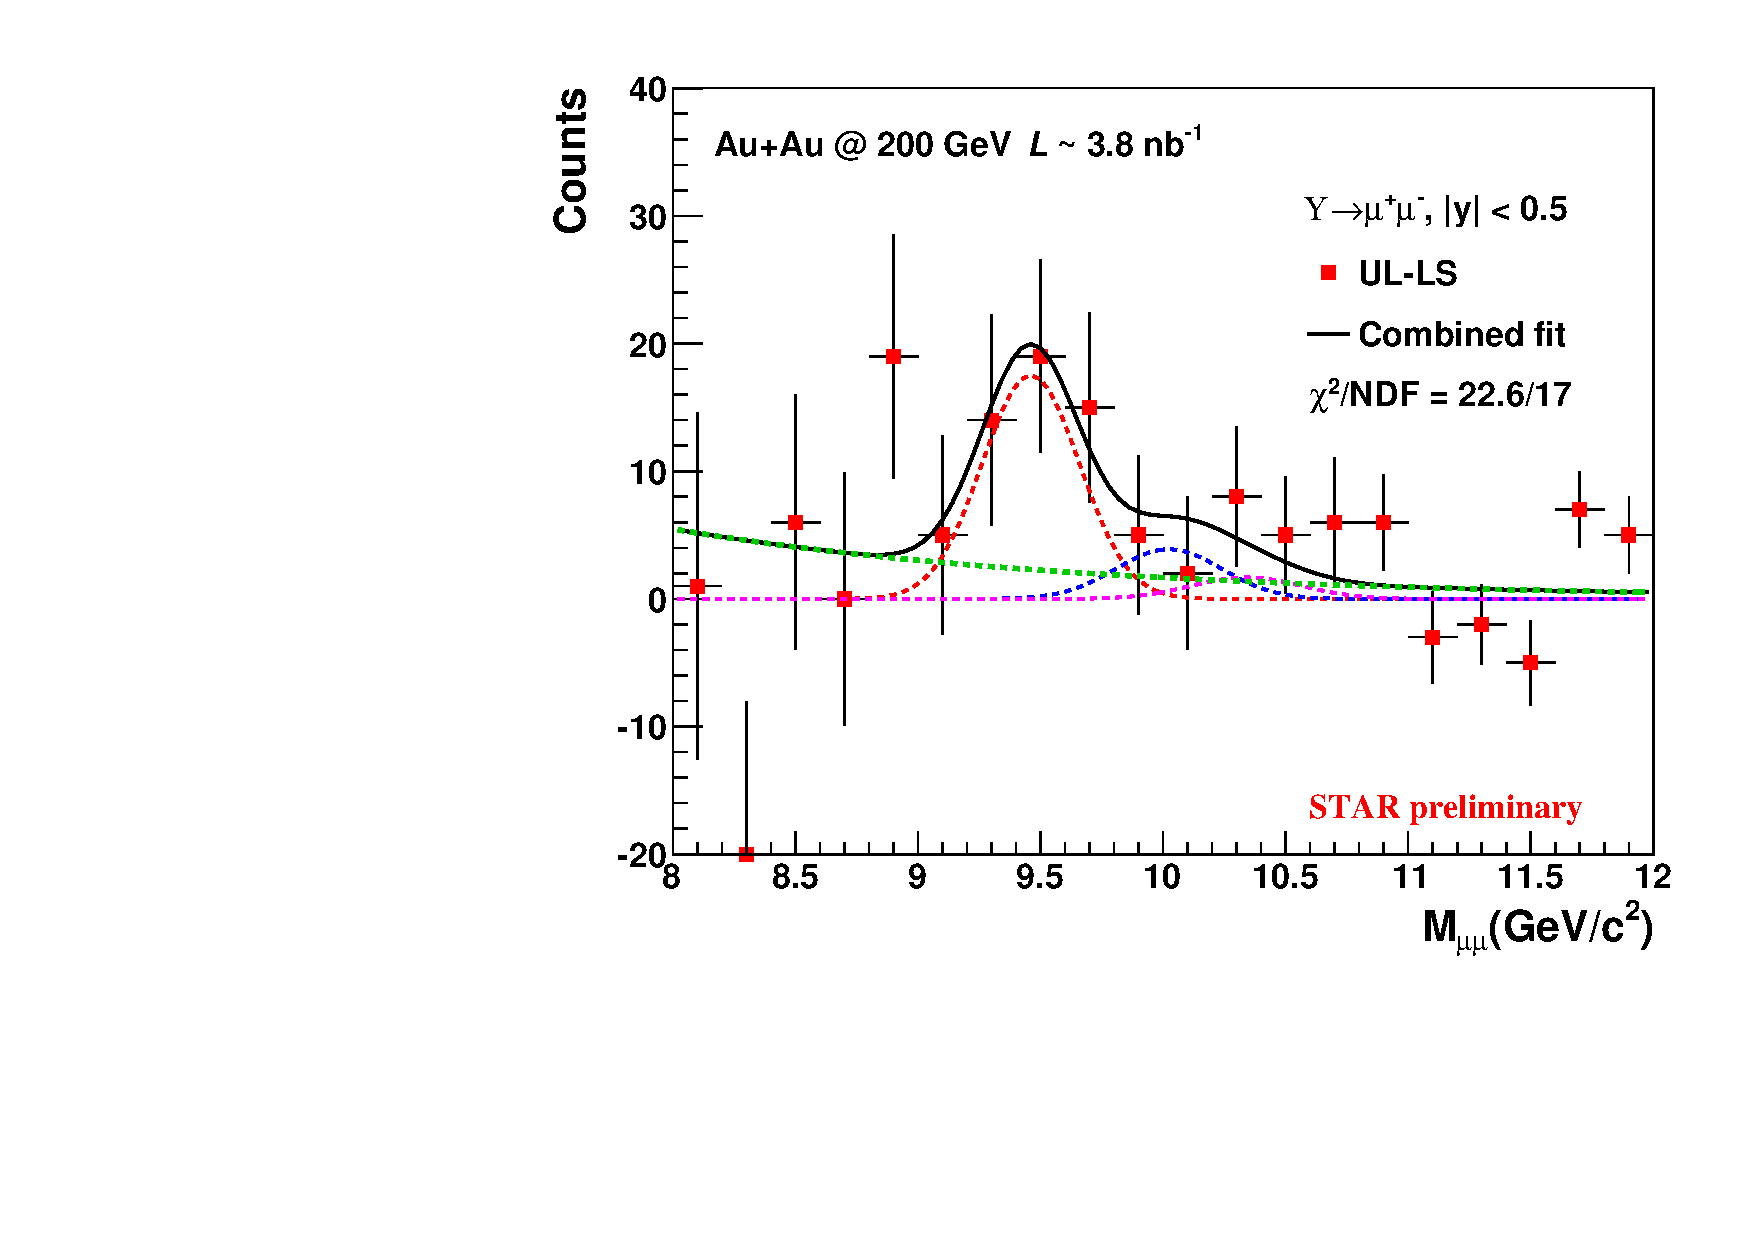
\includegraphics[angle=-90,width=1.0\textwidth]{mtd/Run14_Upsilon.pdf}
\caption{ Invariant mass distribution of unlike-sign dimuon pairs after subtracting the like-sign distribution (red points).
A combined fit of signal and residual background ($b\overline{b}$ + Drell-Yan) is shown as the solid black curve.\label{upsilonviamumu}}
\end{minipage}
\hfill
\begin{minipage}[htbp]{0.48\linewidth}
\centering
\includegraphics[angle=-90,width=1.0\textwidth]{mtd/Run14_Upsilon_Ratio_log.pdf} 
\caption{The projection of ($\varUpsilon_{2S}$ + $\varUpsilon_{3S}$)/($\varUpsilon_{1S}$) using full statistics of Run14 and Run16 Au+Au data collected by the MTD, together with the published results in different collision systems at different energies~\cite{UpsilonWorldwide, UpsilonSTAR, UpsilonCMS}.\label{upsilonproj}}
\end{minipage}
\end{figure}

We are still investigating the characteristics of hadrons recorded by the MTD and developing a better muon identification method. Once a pure muon sample can be identified, the di-$\mu$ and e-$\mu$ spectra using the full-statistics 200 GeV Au + Au data will be measured, which will provide a direct access to the QGP thermal radiation.

%封面是按照制本厂的要求制作的,其中行宽和行高都是固定的,中文标题最多占两行,英文标题最多占三行。如果您的题目超过了这个限制,请缩减题目长度,不要擅自修改模板中的相关配置参数。


  \chapter{Dielectron Analysis Details}
\label{chap:analysis}

\section{Event Selection and Centrality Definition}
\label{centrality}
The data set used in this analysis is from U + U collisions at $\sqrt{s_{NN}}$ = 193 GeV in RHIC run year 2012 (Run12). The minimum-bias (MB) trigger is defined as a coincidence between the two VPDs, a coincidence between the two ZDCs, and an online collision vertex cut. Moreover, a pile-up protection at the trigger level was applied for the data taking.

Events used in this analysis are required to have a valid collision vertex (primary vertex) within 30 cm of the TPC center along $z$ direction (the direction along beam axis) to ensure uniform a TPC acceptance. Furthermore, the distance between the collision vertex along $z$ direction constructed by the TPC ($V_{z}^{TPC}$) and the VPD ($V_{z}^{VPD}$, fast detector) is within 3 cm to reject the event with wrong reconstructed TPC vertex from different bunch-crossing collisions. To reject the events from the beam hitting the beam pipe, vertex with a radial length less than 2 cm with respect to the beam pipe center is required. After event selection, 270 million minimum-bias events are finally used in this analysis. Table~\ref{eventselection} lists the event selection criteria.

\begin{table}[htp]
\centering
\caption{Event selection in U + U collisions at 193 GeV.}
\label{eventselection}
\begin{tabular}{c}
\toprule[1.6pt]
Event Selection Criteria \\
\midrule[1.2pt]
\multirow{2}*{$|V_{r}|<$ 2 cm} \\
\\
\multirow{2}*{$|V_{z}^{TPC}|<$ 30 cm} \\
\\
\multirow{2}*{$|V_{z}^{TPC} - V_{z}^{VPD}|<$ 3cm} \\ 
\\  
\bottomrule[1.6pt]
\end{tabular}
\end{table}

The centrality in U + U collisions at 193 GeV is defined using the uncorrected charged particle density ($dN_{ch}/dy$). The primary tracks with $|\eta|$ $\leq$ 0.5, dca $\leq$ 3 cm and nHitsFit $\geq$ 10 (number of hits used for track fitting) are used to calculate the $dN_{ch}/dy$. Furthermore, the $dN_{ch}/dy$ is corrected for the $V_{z}^{TPC}$ and luminosity dependence to account for the acceptance and efficiency changes on the measured $dN_{ch}/dy$. Then the $dN_{ch}/dy$ is compared to a Monte Carlo (MC) Glauber calculation~\cite{MCGlauber} to delineate the centrality bins, the equivalent number of binary nucleon + nucleon collisions ($N_{bin}$ or $N_{coll}$) and the number of participants ($N_{part}$) for nucleus + nucleus collisions. Table~\ref{centrality} lists the $\langle$$N_{coll}$$\rangle$ and $\langle$$N_{part}$$\rangle$ from Glauber model for each defined centrality bin in U + U collisions at $\sqrt{s_{NN}}$ = 193 GeV. The 0-80\% and finer centrality-bins within this range are used in this analysis, because the 80-100\% centrality has significant trigger bias due to vertex inefficiency at low charged particle density.  

\begin{table}[htp]
\centering
\caption{Centrality bins and corresponding $\langle$$N_{coll}$$\rangle$, $\langle$$N_{part}$$\rangle$ in U + U at 193 GeV.}
\label{centrality}
\newcolumntype{V}{!{\vrule width 1.6pt}}
\begin{tabular}{Vc|r@{.}l|r@{.}lVc|r@{.}l|r@{.}lV}
\Xhline{1.6pt}
Centrality & \multicolumn{2}{c|}{$\langle$$N_{coll}$$\rangle$} & \multicolumn{2}{cV}{$\langle$$N_{part}$$\rangle$} & Centrality & \multicolumn{2}{c|}{$\langle$$N_{coll}$$\rangle$} & \multicolumn{2}{cV}{$\langle$$N_{part}$$\rangle$} \\
\Xhline{1.2pt}
0-5\% & 1281&26 & 414&87 & 5-10\% & 1010&97 & 355&42 \\ \hline
10-15\% & 798&53 & 300&92 & 15-20\% & 628&01 & 253&66 \\ \hline
20-25\% & 490&60 & 212&84 & 25-30\% & 379&86 & 177&48 \\ \hline
30-35\% & 290&31 & 146&78 & 35-40\% & 217&35 & 119&63 \\ \hline
40-45\% & 160&03 & 96&34 & 45-50\% & 115&69 & 76&43 \\ \hline
50-55\% & 81&76 & 59&55 & 55-60\% & 56&98 & 45&73 \\ \hline
60-65\% & 38&36 & 34&01 & 65-70\% & 25&06 & 24&55 \\ \hline
70-75\% & 16&28 & 17&46 & 75-80\% & 10&23 & 11&98 \\ \hline
\Xhline{1.6pt}
\end{tabular}
\end{table}

\section{Electron Identification}

\subsection{Track Selection}
The interested electrons (including positrons if not specified) are mainly from the collision point or short-lived particle decays close to the collision point. Thus the primary tracks, including the primary vertex for the track fitting resulting in a better momentum resolution, are used in this analysis. The primary tracks are required to satisfy the following selection criteria: $p_{T}$ is $\geq$ 0.2 GeV/$c$ to ensure that the track can pass through the TPC; the Distance of Closest Approach (dca) to the primary vertex is $\leq$ 1 cm to reduce contributions from secondary decays; the number of hit points (nHitsFit) along the track is $\geq$ 20 (of a maximum of 45) to ensure good momentum resolution; the ratio of number of hit points along the track over the number of maximum possible points (nHitsPoss) is $\geq$ 0.52 to suppress the possibility of selecting duplicated short tracks from track splitting; the number of points used for calculating $\langle$$dE/dx$$\rangle$ (nHitsDedx) is $\geq$ 15 to ensure good $dE/dx$ resolution; at last, the track is required to match with the TOF and restricted to $|\eta|$ $\leq$ 1.
 
\subsection{Electron Identification Cuts}

The electron candidates could be identified by combining the TPC and TOF. The TPC provides particle identification utilizing the $dE/dx$, because different particle species with the same momentum may have different $dE/dx$. However, in some momentum regions, the TPC can not identify different particle species with very similar $dE/dx$ (e.g. $e/K$ at p $\approx$ 0.5 GeV/$c$, $e/p$ at p $\approx$ 1 GeV/$c$). Different particle species with the same momentum have different velocities, thus the TOF with $<$80 ps time resolution can be used to identify different particle species in the $dE/dx$ crossover regions by precise velocity information ($1/\beta$ = $ct/l$). The normalized $dE/dx$, defined in Eq.~\ref{nsigmae:eq}, instead of $dE/dx$ is used in this analysis. Where $\langle{dE/dx}\rangle^{Mea.}$ and $\langle{dE/dx}\rangle^{Th.}_{e}$ represent measured and theoretical $dE/dx$, and $R_{dE/dx}$ is the STAR TPC $dE/dx$ resolution (typically $\sim$8\%). If the $dE/dx$ (truncated $dE/dx$) calibration is done perfectly, the $n\sigma_{e}$ of electron sample should be close to a standard Gaussian distribution (mean $=$ 0, $\sigma = $ 1).
\begin{equation}
n\sigma_e = \frac{1}{R_{dE/dx}}log\frac{\langle{dE/dx}\rangle^{Mea.}}{\langle{dE/dx}\rangle^{Th.}_{e}}
\label{nsigmae:eq}
\end{equation}

By applying the TOF velocity cut, the slow hadrons are rejected from electrons in the $dE/dx$ overlapping regions, as shown in Fig.~\ref{beta}. After the TOF velocity cut, the $n\sigma_{e}$ cut is applied to reject hadrons with almost the same velocity as electrons, as shown in Fig.~\ref{nsigmae:cut}. The electron sample is then extracted. A tachyon band is observed in the Fig.~\ref{beta}, that is because TOF hits from electrons originating from photon conversions in the material between the TPC and TOF leaving no trace in the TPC are randomly associated with TPC tracks especially in high-multiplicity collisions~\cite{STAR:dielectron1,dielectronJie}. The random match could also result in some slow hadrons surviving the TOF velocity cut. Besides the random match, the secondary particles with inaccurate track length and flight time measurement may also survive the TOF velocity cut. For those survived slow hadrons, if their $dE/dx$ overlap with electrons, there is no way to reject them, as shown in Fig.~\ref{nsigmae:cut}. Thus the electron purity should be estimated, as discussed in Sec.~\ref{purity}. For the systematic uncertainty study from hadron contamination, it will be discussed in Sec.~\ref{sysUncertainty}. Table.~\ref{eid} lists the track selection criteria and electron identification cuts. The $n\sigma_{e}$ distribution of the pure electron sample is centered at -0.34 instead of 0 due to the imperfect TPC calibration, as shown in Fig.~\ref{pureelectron}. Thus the $n\sigma_{e}$ cut is shift down 0.34 to account for this effect.

\begin{figure}[htbp]
\begin{minipage}[htbp]{0.48\linewidth}
\centering
\includegraphics[width=1.0\textwidth]{analysis/betavsp.png}
\caption{$1/\beta$ vs. particle momentum distribution.\label{beta}}
\end{minipage}
\hfill
\begin{minipage}[htbp]{0.48\linewidth}
\centering
\includegraphics[width=1.0\textwidth]{analysis/nsigmaevsp.png} 
\caption{$n\sigma_{e}$ vs. particle momentum after the high velocity cut applied, as shown in Fig.~\ref{beta}.\label{nsigmae:cut}}
\end{minipage}
\end{figure}

\begin{table}[htp]
\centering
\caption{Electron candidates selection criteria.}
\label{eid}
\newcolumntype{V}{!{\vrule width 1.6pt}}
\begin{tabular}{cVc}
\Xhline{1.6pt}
\thead{\small{Track Quality} \\ \small{Cuts} } &  \thead{ \small{Electron Identification} \\ \small{Cuts} } \\
\Xhline{1.2pt}
0.2 $\leq$ $p_{T}$$\leq$ 30 GeV/$c$ & \multirowcell{2}{p $<$ 1 GeV/$c$, \\ 1.5625$\times$(p - 0.2) - 2 \textbf{- 0.34} $\leq$ $|n\sigma_{e}|$ $\leq$ 2 \textbf{- 0.34}}\\ 
$|\eta|$ $\leq$ 1 & \\ 
nHitsFit $\geq$ 20 & \multirowcell{2}{p $\geq$ 1 GeV/$c$, \\ -0.75 \textbf{- 0.34} $\leq$ $|n\sigma_{e}|$ $\leq$ 2 \textbf{- 0.34}} \\
nHitsFit/nHitsPoss $\geq$ 0.52 & \\ 
nHitsDedx $\geq$ 15 & \multirow{2}*{ $|1 - 1/\beta|$ $\leq$ 0.025} \\
dca $\leq$ 1 cm & \\
\Xhline{1.6pt}
\end{tabular}
\end{table}

\subsection{Electron Purity}
\label{purity}
The pure hadron samples ($\pi/K/p$) are selected by combining tight $m^{2}$ and loose $n\sigma_{hadron}$ cuts. The selection criteria and $n\sigma_{e}$ distribution for each pure hadron sample are shown in Fig.~\ref{purehadron}. The pure electron sample is from the $\pi^{0}$ Dalitz decay and photon conversion. The invariant mass of the electron pair from photon conversion should be zero. However, the primary track, forced to originate from primary vertex, is used to reconstruct the electron pair invariant mass (see detailed procedure in Sec.~\ref{invmass}). That will introduce a artificial opening angle between electron and positron resulting in a non-zero invariant mass. The angle depends on the distance between the photon conversion point and the primary vertex. Thus the photons converting at different positions result in different invariant mass. The $M_{ee} <$ 0.015 GeV/$c^{2}$ is used to select the $\pi^{0}$ Dalitz decayed and photon conversion electrons with 148:1 signal-to-background ratio, shown in the left panel of Fig.~\ref{pheselection}. After subtracting the same sign electron pairs from the opposite sign electron pairs, shown in the right panel of Fig.~\ref{pheselection}, the pure electron sample is thus extracted, shown in Fig.~\ref{pureelectron}. Due to the high charged particle density in U + U collisions at 193 GeV, it is likely to happen that two tracks with same charge and similar momentum are very closed to each other. The two tracks are very likely to be reconstructed into ``one track'' due to the finite hit position resolution, so called ``merged track''. The pion is very abundant in U + U collisions at 193 GeV, thus the ``merged $\pi$'' should be taken into account for the purity study. The ``merged $\pi$'' could be selected using the same $m^{2}$ cut as normal $\pi$ but with $n\sigma_{\pi} >$ 6 (``merged $\pi$'' is with doubled $dE/dx$ compared to a normal $\pi$). The $n\sigma_{e}$ distribution of each selected pure sample could be fitted by Gaussian function in each fine $p_{T}$ bin. The mean and sigma of the $n\sigma_{e}$ distribution for each pure sample are shown in Fig.~\ref{puresamplemeansigma}. The electron purity is then estimated based on multi-Gaussian fitting while the mean and width of each component is constrained by the values in Fig.~\ref{puresamplemeansigma}. Figure~\ref{multigaus} shows an example of the multi-Gaussian fitting. In the $dE/dx$ overlap region, the multi-Gaussian fitting is not reliable. An exponential function is employed to extrapolate the hadron particle yields in the overlapping regions as shown in the left panel of  Fig.~\ref{particleyield}. The hadron yields are then constrained, just leaving the electron yield as a free parameter, in the multi-Gaussian function for refitting. The electron yield from the second-round multi-Gaussian fitting is extracted to check the fit reliability, shown in the right panel of Fig.~\ref{particleyield}. The electron purity difference between these two-round fittings is taken as the systematic uncertainty. Figure~\ref{electronpurity} shows the electron purity (overall at $\sim$95\%) in U + U minimum-bias collisions at 193 GeV.

\begin{figure}
\centering
\vspace*{-3mm}
\includegraphics[width=0.48\textwidth]{analysis/pikpsample.eps}
\hspace*{-5mm}
\includegraphics[width=0.48\textwidth]{analysis/PinSigEvsP.png}
\includegraphics[width=0.48\textwidth]{analysis/knSigEvsP.png}
\hspace*{-5mm}
\includegraphics[width=0.48\textwidth]{analysis/PnSigEvsP.png}
\figcaption{The selection criteria and $n\sigma_{e}$ distribution as a function of momentum for each pure hadron sample in U + U 193 GeV minimum-bias collisions. (Top Left) $m^{2}$ distribution of different particle species and pure hadron $m^{2}$ selection criteria. (Top Right) Pure pion sample. (Bottom Left) Pure kaon sample. (Bottom Right) Pure proton sample.}
\label{purehadron}
\end{figure}

\begin{figure}
\centering
\includegraphics[width=0.48\textwidth]{analysis/PHE.eps}
\includegraphics[width=0.48\textwidth]{analysis/PHE_UL_Like.eps}
\figcaption{The selection criteria and $n\sigma_{e}$ distribution of pure electron sample in U + U minimum-bias collisions at 193 GeV. (Left) The invariant mass distribution of $\pi^{0}$ Dalitz decay and photon conversion electron pairs. (Right) The $n\sigma_{e}$ distribution of $\pi^{0}$ Dalitz decay and photon conversion electrons.}
\label{pheselection}
\end{figure}

\begin{figure}[htbp]
\centering
\includegraphics[keepaspectratio,width=0.6\textwidth]{analysis/mean_of_nsigmae_vs_pt_4electron.eps}
\figcaption{The $n\sigma_{e}$ distribution of pure electron sample as a function of momentum in U + U minimum-bias collisions at 193 GeV. The mean of the $n\sigma_{e}$, shown as black dots, is shift to -0.34 due to imperfect TPC $dE/dx$ calibration.}
 \label{pureelectron}
\end{figure}

\begin{figure}
\centering
\includegraphics[width=0.48\textwidth]{analysis/mean_of_nsigmae_vs_pt.eps}
\includegraphics[width=0.48\textwidth]{analysis/sigma_of_nsigmae_vs_pt.eps}
\figcaption{The mean (Left) and sigma (Right) of the $n\sigma_{e}$ for each pure particle sample as a function of momentum in U + U 193 GeV minimum-bias collisions.}
\label{puresamplemeansigma}
\end{figure}

\begin{figure}[htbp]
\centering
\includegraphics[keepaspectratio,width=0.5\textwidth]{analysis/multi_Gaussian_fit.eps}
\figcaption{The $n\sigma_{e}$ distribution after the TOF velocity cut and the multi-Gaussian fit result in momentum bin (0.64, 0.68) GeV/$c$.}
 \label{multigaus}
\end{figure}

\begin{figure}[htbp]
\centering
\includegraphics[width=0.48\textwidth]{analysis/Fit_Interpolate_ConstValue.eps}
\includegraphics[width=0.48\textwidth]{analysis/Econst_crosscheck.eps}
\figcaption{(Left) The yields (solid markers) for different particle species extracted from first-round multi-Gaussian fitting as a function of momentum. The gray areas (left: $e/K$, right: $e/p$) depict the $dE/dx$ crossover regions. The solid lines are the exponential fits for extrapolating the hadron yields (open markers) in the crossover regions. (Right) The electron yields (the only free parameter) from the second-round multi-Gaussian fitting to check the fitting reliability.}
\label{particleyield}
\end{figure}

\begin{figure}[htbp]
\centering
\includegraphics[keepaspectratio,width=0.5\textwidth]{analysis/Electron_Pur.eps}
\figcaption{The electron purity in U + U minimum-bias collisions at 193 GeV, the green band represents the systematic uncertainties.}
 \label{electronpurity}
\end{figure}


\section{Pair Reconstruction and Background Subtraction}
\label{invmass}
The foreground (also called unlike-sign pairs, $N_{+-}$, including signal and background) is reconstructed by combining the electron and positron candidates in the same event. The invariant mass ($M_{ee}$) of the electron pairs are calculated by Eq.~\ref{mass}, 
\begin{equation}
M_{ee} = \sqrt{ (E_{+} + E_{-})^{2} - (\overrightarrow{p}_{+} + \overrightarrow{p}_{-})^{2}}
\label{mass}
\end{equation}
where $E_{+/-} = \sqrt{m_{e}^{2} + \overrightarrow{p}_{+/-}^{2}}$, $m_{e}$ = 0.511 MeV/$c^{2}$ and $\overrightarrow{p}_{+/-}$ are measured by the TPC. The signals come from the Drell-Yan production, quarkonia decay, QGP thermal radiation, heavy flavor semi-leptonic decay, vector mesons in-medium decay and long-lived hadron decays. The background sources include the combinatorial background, correlated background and photon conversions. The combinatorial background comes from uncorrelated electron and positron pairing while the correlated background comes from correlated electron and positron pairing; for example, pairs from Dalitz decay followed by a conversion of the decayed photon (e.g. $\pi^{0} \rightarrow \gamma + e^{+} + e^{-} \rightarrow e^{+} + e^{-} + e^{+} + e^{-}$) or jets (e.g. electron and positron are from same-jet fragmentation or back-to-back di-jet fragmentation). The photon conversion background is from the photon interacting with the detector material and converting into an electron-positron pair. The reconstruction and subtraction of these three background sources are discussed in following sections.

%\begin{figure}[htbp]
%\centering
%\includegraphics[keepaspectratio,width=1.0\textwidth]{analysis/hephivsp.png}
%\figcaption{The $\phi$ vs. $p_{T}$ distributions for electron and positron candidates. The blank strips are caused by the read-out sector boundaries. The bad TPC sector (sector 7, in positive $\eta$ region) is constrained by the black solid lines.}
% \label{ephivspt}
%\end{figure}

\begin{figure}[htbp]
\begin{minipage}[htbp]{0.49\linewidth}
\centering
\includegraphics[width=1.0\textwidth]{analysis/hephivsp.png}
\caption{The $\phi$ vs. $p_{T}$ distributions for electron and positron candidates. The blank strips are caused by the read-out sector boundaries. The bad TPC sector (sector 7, in positive $\eta$ region) is constrained by the black solid lines.\label{ephivspt}}
\end{minipage}
\hfill
\begin{minipage}[htbp]{0.49\linewidth}
\centering
\includegraphics[width=1.0\textwidth]{analysis/acceptance1D.eps} 
\caption{The 1-D acceptance correction factor as a function of $M_{ee}$ in Run12 U + U  minimum-bias collisions at 193 GeV.\label{acc1d}}
\end{minipage}
\end{figure}

\subsection{Like-sign Technique}
\label{likesign}

The like-sign technique, combining same charge sign electrons into pairs in the same event ($N_{++}$ and $N_{--}$), is used to account for the combinatorial and correlated backgrounds. The geometric mean of the like-sign pairs 2$\sqrt{N_{++} \bm\cdot N_{--}}$, demonstrated  in~\cite{PHENIX:dielectron0}, can fully describe the background in the foreground when the $e^{+}$ and $e^{-}$ are produced in statistically independent pairs. The geometric mean is consistently used in the same-event like-sign background reconstruction. 

%\begin{figure}[htbp]
%\centering
%\includegraphics[keepaspectratio,width=0.8\textwidth]{analysis/acceptance1D.eps}
%\figcaption{The 1-D acceptance correction factor as a function of $M_{ee}$ in Run12 U + U  minimum-bias collisions at 193 GeV.}
 %\label{acc1d}
%\end{figure}

The electrons and positrons are bended into opposite directions owing to the magnetic field. The $\phi$ versus $p_{T}$ of the identified electron and positron candidates is shown in Fig.~\ref{ephivspt}. The blank strips along the $\phi$ direction are caused by the TPC read-out sector boundaries. There is one TPC sector (sector 7, in positive $\eta$ region) with $dE/dx$ calibration issue in Run12 U + U collisions, depicted by the black solid lines in Fig.~\ref{ephivspt}. Thus all the tracks passing through this TPC sector are consistently rejected in this analysis. Due to the magnetic field and the TPC de-active areas (read-out sector boundaries, acceptance holes), the acceptances for the unlike-sign and like-sign pairs are different. The mixed-event technique, discussed in Sec.~\ref{mixedevent}, is employed to correct for this effect. The correction factor is calculated by the ratio of the mixed-event unlike-sign and like-sign distribution in each ($M_{ee}$, $p_{T}^{ee}$) bin and applied in 2-dimension (2-D). The final same-event like-sign background used is calculated by the Eq.~\ref{corrlikesign}, 
\begin{equation}
N_{++\&--}^{corr} = 2\sqrt{N_{++}(M, p_{T}) \bm\cdot N_{--}(M,p_{T})} \times \frac{B_{+-}(M,p_{T})}{2\sqrt{B_{++}(M, p_{T}) \bm\cdot B_{--}(M,p_{T})}}
\label{corrlikesign}
\end{equation}
where $N_{++}$, $N_{--}$, $B_{++}$, and $B_{--}$ represent the distribution of like-sign from the same-event and mixed-event, respectively. $B_{+-}$ represents the distribution of unlike-sign from the mixed-event. $N_{++\&--}^{corr}$ denotes the acceptance-corrected like-sign background from the same-event. Figure~\ref{acc1d} shows the 1-D acceptance correction factor as a function of $M_{ee}$ in Run12 U + U minimum-bias collisions at 193 GeV. 

\subsection{Mixed-Event Technique}
\label{mixedevent}
The like-sign technique, discussed in Sec.~\ref{likesign}, is taken as the best estimation for the combinatorial and correlated backgrounds. However, it is limited to the statistics. The mixed-event technique, combining the electrons and positrons from different events with similar characteristics, is used to reproduce the combinatorial background with improved statistical precision. The data sample is divided into different event pools according to the following event level properties: $z$ position of collision vertex, reference multiplicity, and event plane angle. The collision vertex position and reference multiplicity ensure that the same event pool has similar detector acceptance and efficiency. The event plane angle ensures the same event pool has similar momentum phase space alignment, and further guaranteed by the multiplicity assortment to ensure the events have similar momentum phase space distribution. The second-order event plane angle~\cite{EventPlane0, EventPlane1} is used to sort the events. The $z$ vertex position, form -30 cm to +30 cm, is divided into 10 equidistant bins. The reference multiplicity is divided into 16 bins (0 - 80\%, discussed in Sec.~\ref{centrality}) according to the official StRefMult package provided by STAR. The event plane angle $\Psi$ is divided into 24 equidistant bins. This granularity of the event pools is determined by the same procedure discussed in~\cite{STAR:dielectron1,dielectronJie}. Each event pool holds 100 events at maximum, and one event in the event pool is randomly updated when the pool is full. 

The mixed-event background must be normalized to the acceptance corrected same-event like-sign background. The mixed-event technique can not reproduce the correlated background, thus the normalization factor should be determined in a kinematic region where the same-event like-sign correlated background is negligible. Once the kinematic region selected, the normalization factor and the normalized combinatorial background ($B_{+-}^{comb}$) are calculated via the same method in~\cite{PHENIX:dielectron0} and also shown in Eq.~\ref{normalization}
\begin{equation}
\begin{split}
A_{+} = \frac{\int_{N.R.}N_{++}(M,p_{T})dMdp_{T}}{\int_{N.R.}B_{++}(M,p_{T})dMdp_{T}} \\
A_{-} = \frac{\int_{N.R.}N_{--}(M,p_{T})dMdp_{T}}{\int_{N.R.}B_{--}(M,p_{T})dMdp_{T}} \\
B_{++}^{norm} = \int_{0}^{\infty}A_{+}B_{++}(M,p_{T})dMdp_{T} \\
B_{--}^{norm} = \int_{0}^{\infty}A_{-}B_{--}(M,p_{T})dMdp_{T} \\
B_{+-}^{comb}(M,p_{T}) = \frac{2\sqrt{B_{++}^{norm}B_{--}^{norm}}}{\int_{0}^{\infty}B_{+-}(M,p_{T})dMdp_{T}}B_{+-}(M,p_{T}) 
\label{normalization}
\end{split}
\end{equation}
where N.R. represents the normalization region, $A_{+/-}$ is the like-sign normalization factor in N.R., $B_{++/--}^{norm}$ is the normalized mixed-event like-sign statistics and $B_{+-}^{comb}$ is the normalized mixed-event unlike-sign distribution. Unfortunately the mixed-event technique, working in Au + Au at 200 GeV, does not work in U + U at 193 GeV. There is no flat kinematic region found to do the normalization, as shown in Fig.~\ref{likemixratio}. This may be related to the asymmetric Uranium geometry compared to the symmetric Gold geometry, shown in Fig.~\ref{geometry}. Thus, the same-event like-sign technique is finally used to reconstruct the background in this analysis.

\begin{figure}[htbp]
\centering
\includegraphics[width=0.48\textwidth]{analysis/LMixPosRatio1D.eps}
\includegraphics[width=0.48\textwidth]{analysis/LMixNegRatio1D.eps}
\figcaption{Ratios between same-event and mixed-event like-sign distributions. There is no flat kinematic region to do the mixed-event normalization.}
\label{likemixratio}
\end{figure}

\begin{figure}[htbp]
\centering
\includegraphics[keepaspectratio,width=0.7\textwidth]{analysis/UUGeometry.png}
\figcaption{The spherical Gold nuclei (Left) and the ellipsoidal Uranium nuclei (Right).}
 \label{geometry}
\end{figure}

\subsection{Photon Conversion Removal}
The photon conversion electron pairs are removed from the foreground using the $\phi_{V}$ cut method which is similar to that used by the PHENIX Collaboration~\cite{PHENIX:dielectron0}. The opening angle between the electron and positron from the photon conversion should be 0, and the electron and positron are bent only in the plane perpendicular the magnetic field direction which is along the beam axis $z$ in STAR. The definitions of the unit vector and $\phi_{V}$ angle are shown in the following Eq.~\ref{phiv:eq}:
\begin{equation}
\begin{split}
\stackrel{\wedge}{u}\;= \frac{\overrightarrow{p}_{+} + \overrightarrow{p}_{-}}{|\overrightarrow{p}_{+} + \overrightarrow{p}_{-}|}, \quad
\stackrel{\wedge}v\;= \overrightarrow{p}_{+} \times \overrightarrow{p}_{-} \\
\stackrel{\wedge}w\;=\;\stackrel{\wedge}u \times \stackrel{\wedge}v, \quad
\stackrel{\wedge}w_{c}\;=\;\stackrel{\wedge}u \times \stackrel{\wedge}z \\
cos\phi_{V} = \frac{\stackrel{\wedge}w}{|\stackrel{\wedge}w|} \cdot \frac{\stackrel{\wedge}w_{c}}{|\stackrel{\wedge}w_{c}|}
\label{phiv:eq}
\end{split}
\end{equation}

\begin{figure}[htbp]
\begin{minipage}[htbp]{0.48\linewidth}
\centering
\includegraphics[width=1.0\textwidth]{analysis/sameUnLikeSphiVvsM.eps}
\caption{The $\phi_{V}$ angle vs. invariant mass distribution in Run12 U + U minimum-bias collisions at 193 GeV. The blue solid curve depicts the mass dependent $\phi_{V}$ cut employed to remove the photon conversion electron pairs.\label{phiv:plot}}
\end{minipage}
\hfill
\begin{minipage}[htbp]{0.48\linewidth}
\centering
\includegraphics[width=1.0\textwidth]{analysis/gammaConversionE.eps} 
\caption{Red: the invariant mass distribution of the photon conversion electron pairs. Black: the unlike-sign distribution without $\phi_{V}$ cut. Blue: the unlike-sign distribution with $\phi_{V}$ cut.\label{gammaconversion}}
\end{minipage}
\end{figure}

To illustrate the $\phi_{V}$ angle, a little more explanation is added here. Plane A is defined by mother particle momentum direction and beam axis direction, while plane B is defined by the daughter electron, positron momentum directions. The angle between plane A and plane B is defined as $\phi$ ($0^{\circ} \le \phi \le 90^{\circ}$). According to Eq.~\ref{phiv:eq}, $\phi_{V} = 90^{\circ} -/+\;\phi$. For electron and positron from the photon conversion, $\phi = 90^{\circ}$, thus the $\phi_{V}$ angle is zero or $\pi$. A fixed order between electron and positron is used to calculate the $\phi_{V}$ in this analysis for avoiding $\phi_{V} = \pi$ . There is no preferred orientation for combinatorial electron and positron pairs, and only very weak dependence for electron and positron pairs from hadron decays. Figure~\ref{phiv:plot} shows the $\phi_{V}$ angle as a function of invariant mass in U + U minimum-bias collisions at 193 GeV. The blue solid curve depicts the mass dependent $\phi_{V}$ cut employed to remove the photon conversion electron pairs. Figure~\ref{gammaconversion} shows the invariant mass distribution of the photon conversion electron pairs (red curve). As mentioned before, the different invariant mass peak depicts that the conversion electron pairs are from different materials. The mass shifted from zero is because the electrons are assumed to originate from the primary vertex during the final track reconstruction. Therefore, the two main peaks (for the red histogram) from low to high mass correspond to the conversion from the beam pipe and inner cone support structure, respectively.

\subsection{Raw Signal}
The background, in this analysis, is subtracted by the same-event like-sign technique. The same-event like-sign distribution is firstly corrected for the acceptance and then subtracted from the inclusive unlike-sign (foreground) distribution. The invariant mass distribution of signal pairs before detector efficiency losses correction (raw signal) is thus obtained. The upper panel of Fig.~\ref{rawsignal} shows the invariant mass distributions of foreground (black dots), background (black line) and raw signal (blue dots), while the bottom panel shows the signal-to-background ratio in U + U  minimum-bias collisions at $\sqrt{s_{NN}}$ = 193 GeV.

\begin{figure}[htbp]
\centering
\includegraphics[keepaspectratio,width=0.8\textwidth]{analysis/rawSignal_SBRatio.eps}
\figcaption{(Top) The invariant mass distributions of raw signal (blue dots), foreground (black dots) and background (black line). (Bottom) The signal-to-background ratio in U + U  minimum-bias collisions at $\sqrt{s_{NN}}$ = 193 GeV.}
 \label{rawsignal}
\end{figure}

\section{Efficiency and Acceptance Corrections}
To obtain the real invariant mass spectrum of dielectron within STAR acceptance ($p_{T}^{e} \geq 0.2\;GeV/c, |\eta_{e}| \leq 1, |Y_{ee}| \leq 1$), the raw spectrum should be corrected for the efficiency losses. The pair efficiency within STAR acceptance is evaluated by folding the single track efficiency. To measure the dielectron excess yield and study the medium properties, the dielectron excess spectrum (dielectron invariant mass spectrum with hadronic contributions except $\rho$-meson subtracted, see details in Sec.~\ref{cocktail}) is needed to be corrected for the detector acceptance.

\subsection{Single Track Efficiency}
\label{singletrkeff}
The single track efficiency losses are caused by the detector inefficiency and electron identification cuts. The detector efficiency includes the TPC tracking efficiency ($\varepsilon_{TPC}$), nHitsDedx cut efficiency ($\varepsilon_{nHitsDedx}$) and the TOF matching efficiency ($\varepsilon_{TOF}$). The electron identification cut efficiency ($\varepsilon_{eID}$) includes the efficiencies of TOF velocity and the $dE/dx$ selection cuts. So the single track efficiency can be derived by the Eq.~\ref{singleeff}
\begin{equation}
\varepsilon_{e} = \varepsilon_{TPC} \times \varepsilon_{nHitsDedx} \times \varepsilon_{TOF} \times \varepsilon_{eID}
\label{singleeff}
\end{equation}
Each part will be discussed in the following sub-sections.

\subsubsection{TPC Tracking Efficiency}
\label{embedding}
The TPC tracking efficiency ($\varepsilon_{TPC}$), including the TPC response and acceptance, is evaluated via the standard STAR embedding technique. The Monte Carlo (MC) tracks are embedded into the read data at the raw data level to have a realistic detector occupancy environment. The real data is randomly sampled over the entire U + U minimum-bias data set, while the number of embedded MC tracks is constrained to 5\% of the measured multiplicity of the real events to avoid a sizable impact on the realistic TPC tracking efficiency. The MC tracks, with flat $p_{T}$, $\eta$, and $\phi$, are generated and passed through the full simulation of the STAR detector geometry using the GEANT model~\cite{GEANT}, and then mixed with the real data . The mixed signals are processed using the exactly same off-line reconstruction chain. The quality assurance is made to ensure the MC simulation reproduces the real data before studying the TPC tracking efficiency, The TPC tracking efficiency is derived by taking the ratio of the number of reconstructed MC tracks ($N_{rec}$), satisfying the track quality cuts except nHitsDedx cut used in the data analysis, over the number of embedded MC tracks ($N_{emb}$), as shown in Eq.~\ref{tpceff}
\begin{equation}
\varepsilon_{TPC} = \frac{N_{rec}\;(nHitsFit\geq20\;\&\;\frac{nHitsFit}{nHitsPoss}\geq0.52\;\&\;dca\leq1\;\&\;|\eta|\leq1)}{N_{emb}\;(|\eta|\leq1)}
\label{tpceff}
\end{equation}
The 1-D TPC tracking efficiency in Run12 U + U minimum-bias collisions at 193 GeV is shown in Fig.~\ref{1dtpceff}. However, the 3-D ($p_{T}$, $\eta$, and $\phi$) TPC tracking efficiency will be used in the finally pair efficiency correction, discussed in Sec.~\ref{paireff}.

\subsubsection{nHitsDedx Cut Efficiency}
The nHitsDedx cut efficiency ($\varepsilon_{nHitsDedx}$) is derived from the real data, because the nHitsDedx variable from MC simulation is not consistent with the data. The photonic electron sample (using all track quality and eID cuts except nHitsDedx and the TOF velocity cuts) is selected according to the method discussed in  Sec.~\ref{purity}. The TOF velocity cut is abandoned, because it biases the nHitsDedx to a large number due to the TOF matching algorithm. The nHitsDedx cut efficiency is then derived by comparing the number of photonic electron tracks with and without nHitsDedx cut. Figure~\ref{nhitsdedxeff} shows the nHitsDedx cut efficiency as a function of $p_{T}$ in Run12 U + U minimum-bias collisions at 193 GeV.

\begin{figure}[htbp]
\begin{minipage}[htbp]{0.48\linewidth}
\centering
\includegraphics[width=1.0\textwidth]{analysis/TpcEff_MB.eps}
\caption{The 1-D TPC tracking efficiency in Run12 U + U minimum-bias collisions at 193 GeV.\label{1dtpceff}}
\end{minipage}
\hfill
\begin{minipage}[htbp]{0.48\linewidth}
\centering
\includegraphics[width=1.0\textwidth]{analysis/PHE_nHitsDedxEff.eps} 
\caption{The nHitsDedx cut efficiency in Run12 U + U minimum-bias collisions at 193 GeV.\label{nhitsdedxeff}}
\end{minipage}
\end{figure}

\subsubsection{TOF Matching Efficiency}
The TOF matching efficiency ($\varepsilon_{TOF}$), including the TOF response and the acceptance difference between the TPC and TOF, is evaluated by the real data. It can be calculated by comparing the number of qualified primary tracks matched with the TOF (with $\beta$ > 0, $N_{matched}$) over  the number of qualified primary tracks ($N_{TPC}$). Due to the limited statistics of  pure electron sample, the pure pion sample selected by a tight TPC $dE/dx$ cut (|$n\sigma_{\pi}$| < 0.6), is thus used to generate the 3-D ($p_{T}$, $\eta$, and $\phi$) TOF matching efficiency. The TOF matching efficiency difference between the electron and pion is then corrected for each ($\eta$, $\phi$) bin using the same $p_{T}$ dependent correction factor. The TOF matching efficiency difference between electrons and pions, is due to the decay loss of pions between the TPC and TOF as well as other effects (e.g. pile-up effect). The 1-D TOF matching efficiency and the $p_{T}$ dependent correction factor are shown in Fig.~\ref{tofeff}.

\begin{figure}[htbp]
\centering
\includegraphics[width=0.48\textwidth]{analysis/PHE_Pion_TofEff.eps}
\includegraphics[width=0.48\textwidth]{analysis/PHE_Pion_TofEffRatio.eps}
\figcaption{(Left) The 1-D TOF matching efficiency for pure electron and pion sample in Run12 U + U minimum-bias collisions at 193 GeV. (Right) The corresponding TOF matching efficiency ratio of electron over pion as a function of $p_{T}$.}
\label{tofeff}
\end{figure}

\subsubsection{eID Cuts Efficiency}
\label{eideff}
The electron identification cut efficiency ($\varepsilon_{eID}$) includes two components: the TOF velocity ($1/\beta$) cut efficiency and $dE/dx$ cut ($n\sigma_{e}$) efficiency. Pure electron sample is used to evaluate the TOF velocity cut efficiency, and the $1/\beta$ distribution of the pure electron is shown in the left panel of Fig.~\ref{betaeff}. The red lines depict the $1/\beta$ cut used in this analysis, and the efficiency is calculated using two methods: a Gaussian fit the $1/\beta$ distribution and direct counting for each $p_{T}$ bin. The Gaussian fit overestimates the $1/\beta$ cut efficiency due to the tail structure in each $p_{T}$ bin. Thus the default $1/\beta$ cut efficiency value, shown in the right panel (blue circles) of Fig.~\ref{betaeff}, comes from the direct counting method, and the difference between this two methods is taken into account for the systematic uncertainty. The $n\sigma_{e}$ cut efficiency is derived from the multi-Gaussian fit discussed in Sec.~\ref{purity}. Figure~\ref{nsigmaeeff} depicts the $n\sigma_{e}$ cut efficiency in Run12 U + U minimum-bias collisions at 193 GeV.

\begin{figure}[htbp]
\centering
\includegraphics[width=0.48\textwidth]{analysis/PHE_beta.png}
\includegraphics[width=0.48\textwidth]{analysis/Beta_CutEff_Minus1.eps}
\figcaption{(Left) The $1/\beta$ distribution for pure electron sample in Run12 U + U minimum-bias collisions at 193 GeV. Red dashed lines represent the $1/\beta$ cut used in this analysis. Black dots represent the $1/\beta_{mean}$ for each $p_{T}$ bin while the black curve is the fit function. (Right) The $1/\beta$ cut efficiencies using bin counting (default, blue circles) and Gaussian fit (black dots) methods.}
\label{betaeff}
\end{figure}

\begin{figure}[htbp]
\centering
\includegraphics[keepaspectratio,width=0.6\textwidth]{analysis/nSigEcut4TpcE_Eff.eps}
\figcaption{The $n\sigma_{e}$ cut efficiency in U + U  minimum-bias collisions at 193 GeV.}
 \label{nsigmaeeff}
\end{figure}

\subsection{Pair Efficiency and Acceptance}
\label{paireff}

\paragraph{Pair Efficiency}
The dielectron pair efficiency within STAR acceptance ($p_{T}^{e}$ $\geq$ 0.2 GeV/$c$, $|\eta_{e}|$ $\leq$ 1, $|Y_{ee}|$ $\leq$ 1) is evaluated from single track efficiency by two different simulation folding methods:
\begin{itemize}
\item[(i)] Toy MC simulation (Virtual photon simulation), which uses the virtual photon as input. The 2-D kinematics ($M_{ee}, p_{T}$) of the virtual photon is taken from the hadronic cocktail (discussed in Sec.~\ref{cocktail}) with flat rapidity (Y), azimuthal ($\phi$) distribution, and the virtual photon decays into electron and positron pairs isotropically.
\item[(ii)] Cocktail simulation, which uses the hadronic cocktail as input, including the correlated heavy flavor decay ($c\overline{c}$, $b\overline{b}$) and Drell-Yan process from PYTHIA~\cite{Pythia} simulation. The long-lived hadrons decay into electron and positron pairs isotropically. However, the electron and position from the heavy flavor decay are highly correlated.
\end{itemize} 
The largest difference between these two methods is the correlated heavy flavor contribution, which is still unclear in heavy-ion collisions due to possible medium modifications of the heavy flavor correlations compared to those in $p$ + $p$ collisions. In this analysis, the heavy flavor correlations rely on the PYTHIA simulation without any artificial modification.

The single track efficiencies caused by the TPC tracking and TOF matching are folded into pair efficiency in 3-D ($p_{T}$, $\eta$, and $\phi$) momentum space while the others are folded in 1-D ($p_{T}$) momentum space. The momentum resolution and energy loss effects, discussed in Sec.~\ref{cocktail}, are also taken into account during the folding process. The pair efficiency is calculated and applied in 2-D kinematics ($M_{ee}, p_{T}$). Figure~\ref{paireff2d} shows the 2-D pair efficiency evaluated by the ``Virtual photon simulation'' and ``Cocktail simulation'' methods in Run12 U + U minimum-bias collisions at 193 GeV. Figure~\ref{paireff1d} shows the 1-D pair efficiency comparisons between these two methods, and the differences are pretty small. The default pair efficiency is evaluated by the ``Virtual photon simulation'' and the difference between these two methods is taken into account for systematic uncertainty.  

\begin{figure}[htbp]
\centering
\includegraphics[width=0.48\textwidth]{analysis/pairEff2D_VP_Cen0_80.png}
\includegraphics[width=0.48\textwidth]{analysis/pairEff2D_Cock_Cen0_80.png}
\figcaption{The 2-D pair efficiency evaluated by the ``Virtual photon simulation'' (Left) and ``Cocktail simulation'' (Right) methods in Run12 U + U minimum-bias collisions at 193 GeV.}
\label{paireff2d}
\end{figure}

\begin{figure}[htbp]
\centering
\includegraphics[keepaspectratio,width=0.6\textwidth]{analysis/pairEff1D_AllCens.eps}
\figcaption{The 1-D pair efficiency comparisons between the ``Virtual photon simulation'' (Solid Markers) and ``Cocktail simulation'' (Open Markers) for different centralities in Run12 U + U collisions at 193 GeV.}
 \label{paireff1d}
\end{figure}

The $\phi_{V}$ cut (reject electron pairs) efficiency is evaluated through $\pi^{0}$ Dalitz decay embedding (see Sec.~\ref{embedding}) and the virtual photon simulation. The $\phi_{V}$ cut efficiency obtained by these two methods is shown in Fig.~\ref{phiveff}. The default $\phi_{V}$ cut efficiency is evaluated by the virtual photon simulation and the difference between these two methods is taken into account for the systematic uncertainty.

\begin{figure}[htbp]
\centering
\includegraphics[keepaspectratio,width=0.6\textwidth]{analysis/phiV_eff.eps}
\figcaption{The $\phi_{V}$ angle cut efficiencies obtained by $\pi^{0}$ Dalitz decay embedding and virtual photon simulation.}
 \label{phiveff}
\end{figure}

\begin{figure}[htbp]
\centering
\includegraphics[width=0.48\textwidth]{analysis/Acceptance2D_VP_Cen0_80.png}
\includegraphics[width=0.48\textwidth]{analysis/Acceptance2D_Cock_Cen0_80.png}
\figcaption{The 2-D detector acceptance derived by the ``Virtual photon simulation'' (Left) and ``Cocktail simulation'' (Right) methods in Run12 U + U minimum-bias collisions at 193 GeV.}
\label{acceptance2d}
\end{figure}

\begin{figure}[htbp]
\centering
\includegraphics[keepaspectratio,width=0.6\textwidth]{analysis/Acceptance1D_MB.eps}
\figcaption{The 1-D detector acceptance comparison between the ``Virtual photon simulation'' and ``Cocktail simulation'' in Run12 U + U minimum-bias collisions at 193 GeV.}
 \label{acceptance1d}
\end{figure}

\paragraph{Acceptance}
The efficiency-corrected dielectron spectrum is within STAR acceptance ($p_{T}^{e} \geq 0.2\;GeV/c, |\eta_{e}| \leq 1, |Y_{ee}| \leq 1$). Thus the dielectron excess spectrum (dielectron invariant mass spectrum with hadronic contributions except $\rho$-meson removed. See details in Sec.~\ref{cocktail}) is needed to be corrected for the detector acceptance to quantitatively measure the excess yields and study the medium properties. The acceptance factor is calculated by taking the ratio of dielectron yields after over before filtering STAR acceptance, as shown in the following equation:
\begin{equation}
\varepsilon_{Acc} = \frac{dN/dM_{ee}\;(p_{T}^{e}\geq0.2\;GeV/c\;,\;|\eta_{e}|\leq1\;,\;|Y_{ee}|\leq1)}{dN/dM_{ee}\;(|Y_{ee}|\leq1)}
\label{acceptance:eq}
\end{equation}
The acceptance correction can be evaluated using the same methods (``Virtual photon simulation'', ``Cocktail simulation'' ) described in the pair efficiency correction section. However, the acceptance factors evaluated by these two methods have a huge difference in the IMR, as shown in Fig.~\ref{acceptance2d} and Fig.~\ref{acceptance1d}. The difference is due to the unknown charm correlation which dominates in the dielectron IMR at RHIC energy. In IMR, the correlation of electron pairs is from the pure decay kinematics in the ``Virtual photon simulation'' method while that inherits the correlation of strong correlated charm generated by PYTHIA in ``Cocktail simulation'' method. The acceptance factor evaluated by the ``Virtual photon simulation'' method is finally applied to the excess spectrum, which does not contain the heavy flavor contribution, in 2-D kinematics ($M_{ee}$, $p_{T}$).

\section{Hadronic Cocktail Simulation}
\label{cocktail}
Dielectrons as measured by the detector originate from all stage in the evolution of heavy-ion collisions. The contribution of the dielectron pairs from hadronic decays, so called hadronic cocktail, to the final dielectron spectrum can be well evaluated trough MC simulation once their yields and $p_{T}$ spectra are measured. The components of the cocktail simulation in this analysis are listed below:
\begin{itemize}
\item[(i)] Two-body decays: $\omega \rightarrow e^{+}e^{-}$, $\phi \rightarrow e^{+}e^{-}$, $J/\psi \rightarrow e^{+}e^{-}$, $\psi^{\prime} \rightarrow e^{+}e^{-}$.
\item[(ii)] Dalitz decays: $\pi^{0} \rightarrow \gamma e^{+}e^{-}$, $\eta \rightarrow \gamma e^{+}e^{-}$, $\eta^{\prime} \rightarrow \gamma e^{+}e^{-}$, $\omega \rightarrow \pi^{0}e^{+}e^{-}$, $\phi \rightarrow \eta e^{+}e^{-}$.
\item[(iii)] Heavy-flavor decays: $c\overline{c} \rightarrow e^{+}e^{-}+X$, $b\overline{b} \rightarrow e^{+}e^{-}+X$.
\item[(iv)] Drell-Yan process.
\end{itemize}
The $\rho^{0}$, considered to be modified by the hadronic medium, is excluded in the cocktail simulation. 

For U + U collisions at 193 GeV, there is no measurement for the identified particle species. However, the energy density created in U + U collisions at $\sqrt{s_{NN}}$ = 193 GeV is only about 20\% higher than that in Au + Au collisions at $\sqrt{s_{NN}}$ = 200 GeV~\cite{UUEnergyDensity}. Thus the hadron $p_{T}$ spectra in Au + Au collisions at 200 GeV~\cite{STAR:dielectron1} are employed for cocktail simulation in this analysis, as shown in Fig.~\ref{tbwfit}. The measurements of identified particle species (the symbols in Fig.~\ref{tbwfit}) except $J/\psi$ in Au + Au collisions at 200 GeV, are simultaneously fitted by a core-corona-based Tsallis Blast-Wave (TBW) model~\cite{TBW0, TBW1}. The core and corona describe the bulk production and the hard scattering contributions from $p$ + $p$-like collisions, respectively. The $J/\psi$ is excluded from simultaneously fit, because the $J/\psi$ is not considered as a component of the bulk medium. The TBW fit can well describe the measured light hadron spectra and also provide predictions for the meson species without measurement (e.g. low $p_{T}$ $\eta$, $\eta^{\prime}$, $\omega$) using the same core TBW parameters obtained from the simultaneously fit. The rapidity and azimuthal distribution of the input hadron are assumed to be flat. The yields ($dN/dy$) of the input hadron in Au + Au collisions are extracted  by integrating the fits over the whole $p_{T}$ region.

\begin{figure}[htbp]
\centering
\includegraphics[keepaspectratio,width=0.6\textwidth]{analysis/TBW_AuAu200GeV.eps}
\figcaption{The invariant yields of mesons in Au + Au collisions at 200 GeV. The solid lines show the simultaneous TBW fit to the measured data points (except J/$\psi$) and the TBW predictions for $\eta$, $\eta^{\prime}$, and $\omega$ with the same core TBW parameters. The dashed lines show the TBW fit to the measured J/$\psi$ and the prediction for the $\psi^{\prime}$.}
 \label{tbwfit}
\end{figure}

The $dN/dy$ or cross section ($\sigma$) with their uncertainties and corresponding decay branching ratios of various cocktail components used in Au + Au minimum-bias collisions at 200 GeV, are summarized in~\cite{STAR:dielectron1} (TABLE \uppercase\expandafter{\romannumeral3}). The $dN/dy$ of cocktail hadron components (without measurements) used in U + U minimum-bias collisions at 193 GeV are essentially derived from that of Au + Au minimum-bias collision at 200 GeV by $N_{part}$. The $\pi^{0}$ $dN/dy$ (($\pi^{+} + \pi^{-}$)/2)~\cite{IdentPartYieldsPRCLong} of Au + Au collisions at 200 GeV scaled by $N_{part}/2$ as a function of $N_{part}$, is fitted by a first-order polynomial function. The $\pi^{0}$ $dN/dy$ of U + U collisions at 193 GeV for different centralities are evaluated by this first-order polynomial function, as shown in Fig.~\ref{uupi0yields}. The input $dN/dy$ for other cocktail hadron components (except $J/\psi$ and $\psi^{\prime}$) in U + U minimum-bias collisions at 193 GeV are scaled with the relative pion yields, $R_{\pi^{0}}$ (shown in Tab.~\ref{uupi0}), with respect to Au + Au minimum-bis collisions at 200 GeV. The $dN/dy$ of $J/\psi$ and $\psi^{\prime}$ are scaled by relative $N_{coll}$. The quoted systematic uncertainties of the hadron yields are the same as that of Au + Au collisions at 200 GeV. The input $p_{T}$ spectra of cocktail hadron components for different centralities in U + U collisions at 193 GeV, are also the same as those (using the similar TBW function fit to the available data) of the corresponding centralities in Au + Au collisions at 200 GeV. The heavy flavor contributions to the hadronic cocktail will be discussed later.

\begin{figure}[htbp]
\centering
\includegraphics[keepaspectratio,width=0.6\textwidth]{analysis/AuAuUU_normalized_pi0dNdy_vs_Npart.eps}
\figcaption{The $\pi^{0}$ yields (black dots) scaled by $N_{part}/2$ as a function of $N_{part}$ is fitted by a first-order polynomial function (black line).  The $\pi^{0}$ yields of U + U collisions for different centralities (red stars) are evaluated by this fit function.}
 \label{uupi0yields}
\end{figure}

\begin{table}[htp]
\centering
\caption{The scale factors ($R_{\pi^{0}}$) for different centralities in U + U collisions at 193 GeV, with respect to the $dN_{\pi^{0}}/dy$ (98.49) Au + Au minimum-bias collisions at 200 GeV.}
\label{uupi0}
\begin{tabular}{lr@{.}lr@{.}lr@{.}l}
\Xhline{1.6pt}
Centrality (\%) & \multicolumn{2}{c}{$dN_{\pi^{0}}/dy$} & \multicolumn{2}{c}{$R_{\pi^{0}}$} & \multicolumn{2}{c}{$\langle$$N_{coll}$$\rangle$} \\
\Xhline{1.2pt}
 0-80 & 115&76 & 1&175 & 350&08 \\
 60-80 & 15&72 & 0&160 & 22&48  \\
 40-80 & 33&35 & 0&339 & 63&05  \\
 40-60 & 51&65 & 0&524 & 103&61 \\
 10-40 & 165&90 & 1&684 & 467&44 \\
 0-10 & 358&48 & 3&640 & 1146&12 \\
\Xhline{1.6pt}
\end{tabular}
\end{table}

Once the kinematics ($p_{T}$, $\eta$, and $\phi$) of the parent hadron obtained, the kinematics of the daughter electrons are determined by the decay kinematics. The electron pair mass depends on the parent particle and the decay mode (two-body decay or Dalitz decay). The electron pair mass of two-body decay follows a narrow Breit-Wigner distribution as given in Eq.~\ref{breit:wigner}
\begin{equation}
\frac{dN}{dM_{ee}} = \frac{2\Gamma_{0}}{(M_{ee} - M_{h})^{2} + \Gamma_{0}^{2}/4}
\label{breit:wigner}
\end{equation}
where the $\Gamma_{0}$ represents the PDG~\cite{PDG} width, and $M_{h}$ is the mass of the hadron which decays into the dielectron. The electron pair mass ($M_{ee}$) is constrained to [$2m_{e}$, 4 $GeV/c^{2}$], where the $m_{e}$ is the electron mass. The electron pair mass of Dalitz decay follows the Kroll-Wada formula~\cite{KrollWada} as given in Eq.~\ref{kroll:wada}, 
\begin{equation}
\frac{dN}{dM_{ee}} = PS \cdot |F(M_{ee}^{2})|^{2} \cdot QED
\label{kroll:wada}
\end{equation}
Where PS is the phase space term defined in Eq.~\ref{ps:com}. The $M_{h}$ is mass of the hadron which undergoes a Dalitz decay process ($h \rightarrow Xe^{+}e^{-}$) and $X$ is the third daughter particle with a mass $M_{X}$. if $X$ is massless (e.g. $\gamma$ in $\pi^{0}$, $\eta$, $\eta^{\prime}$ Dalitz decay), the phase space term simplifies to Eq.~\ref{ps:sim}.
\begin{equation}
PS =  \left( (1 + \frac{M_{ee}^{2}}{M_{h}^{2} - M_{X}^{2}})^{2} - \frac{4M_{h}^{2}M_{ee}^{2}}{(M_{h}^{2}-M_{X}^{2})^{2}} \right)^{\frac{3}{2}}
\label{ps:com}
\end{equation}
\begin{equation}
PS =  \left( 1- \frac{M_{ee}^{2}}{M_{h}^{2}} \right)^{3}
\label{ps:sim}
\end{equation}

The QED term is described by Eq.~\ref{qed}, where N represents a degeneracy factor that depends on how many photons can convert. N is 4 for $\omega$ and $\phi$ while it is 2 for other hadrons undergoing Dalitz decay process, involved in this analysis. The $\alpha$ is the fine-structure constant ($\sim$1/137).
\begin{equation}
QED =  \frac{N \cdot \alpha}{3\pi}\sqrt{1-\frac{4m_{e}^{2}}{M_{ee}^{2}}}\left(1 + \frac{2m_{e}^{2}}{M_{ee}^{2}}\right)\frac{1}{M_{ee}}
\label{qed}
\end{equation}

The $F(M_{ee}^{2})$ is the electromagnetic form factor. The form factor, described in Eq.~\ref{formfactor}, is used for almost all Dalitz decay involved in this analysis except $\eta^{\prime}$. 
 \begin{equation}
|F(M_{ee}^{2})|^{2} =  \left(\frac{1}{1 - M_{ee}^{2}\Lambda^{-2}}\right)^{2}
\label{formfactor}
\end{equation}
where the $\Lambda^{-2}$ is the form factor slope, listed in Tab.~\ref{inverselambdasquare}. For $\pi^{0}$ the form factor is usually given by Eq.~\ref{pi0formfactor},
 \begin{equation}
|F(M_{ee}^{2})|^{2} =  \left(1 + M_{ee}^{2}\Lambda^{-2}\right)^{2}
\label{pi0formfactor}
\end{equation}
For $\eta^{\prime}$, the form factor is given by Eq.~\ref{etaprimeformfactor}. The $\Lambda^{-2}$ and $\Gamma_{0}^{2}$ are from the fit to the data presented in~\cite{etaprimeInvLamSqu}, where the $\Lambda^{-2}$ and $\Gamma_{0}^{2}$ are 1.8396 and 1.99 $\times$ $10^{-2}$, respectively. 
 \begin{equation}
|F(M_{ee}^{2})|^{2} =  \frac{1}{(1 - M_{ee}^{2}\Lambda^{-2})^{2} + \Gamma_{0}^{2}\Lambda^{-2}}
\label{etaprimeformfactor}
\end{equation}

\begin{table}[htp]
\centering
\caption{The electromagnetic form factor slope of mesons.}
\label{inverselambdasquare}
\begin{tabular}{cr@{.}l}
\Xhline{1.6pt}
Meson & \multicolumn{2}{c}{$\Lambda^{-2}$} \\
\Xhline{1.2pt}
 $\pi^{0}$ & 1&756~\cite{pi0InvLamSqu} \\
 $\eta$ & 1&95~\cite{etaomegaInvLamSqu} \\
 $\eta^{\prime}$ & 1&8396~\cite{etaprimeInvLamSqu}\\
 $\omega$ & 2&24~\cite{etaomegaInvLamSqu} \\
 $\phi$ & 3&8~\cite{phiInvLamSqu} \\
\Xhline{1.6pt}
\end{tabular}
\end{table}

The correlated heavy flavor contributions ($c\overline{c}$, $b\overline{b}$, and Drell-Yan) to the cocktail are obtained from the PYTHIA~\cite{Pythia} simulation. These three sources are first simulated in $p$ + $p$ collisions and then scaled by $N_{coll}$, listed in Tab.~\ref{uupi0}, to account for the contributions in U + U collisions. The parameter settings (other parameters use the STAR default tune) for different heavy flavors in PYTHIA (version 6.419) are listed below:
\begin{itemize}
\item[(i)] $c\overline{c}$: MSEL = 4 (c trigger), PARP(91) = 1 ($\langle k_{T} \rangle$ = 1.0 GeV/$c$), PARP(67) = 1.0 (parton shower level). 
\item[(ii)] $b\overline{b}$: MSEL = 5 (b trigger), PARP(91) = 1.5 ($\langle k_{T} \rangle$ = 1.5 GeV/$c$).
\item[(iii)] Drell-Yan: MSEL = 11 ($Z_{0}$ or $\gamma^{*}$  trigger), PARP(91) = 1.5 ($\langle k_{T} \rangle$ = 1.5 GeV/$c$).
\end{itemize}
The charm settings are tuned to match the STAR measurement of the charmed-meson spectrum in $p$ + $p$ collisions~\cite{charmedMesonpp}. The input charm-pair production cross section is also from the STAR measurements~\cite{charmedMesonpp, charmedMesonAuAu}. The Drell-Yan setting are tuned to match the theoretical calculation, and the same PYTHIA settings (except trigger setting) are used in the bottom simulation. The input bottom and Drell-Yan production cross sections are $\sigma_{pp}^{b\overline{b}}$ = 37 $\mu$b, $\sigma_{pp}^{DY}$ = 42 nb.

All the physics results reported in Chap.~\ref{chap:result} are not corrected for the STAR detector resolution. It's very challenging to precisely reproduce the momentum resolution through embedding, due to various distortion effects in the TPC in the high luminosity RHIC environment. However, a data-driven method is involved in the hadronic cocktail simulation, accounting for these effects~\cite{STAR:dielectron1}. In the Run12 U + U minimum-bias embedding, the reconstructed electron $p_{T}^{rec}$ probability at a given input $p_{T}^{MC}$ can be described by a double crystal ball function, given in Eq.~\ref{doublecrystal}
\begin{equation} \label{doublecrystal}
P(p_{T}^{rec}, p_{T}^{MC}) \propto 
\begin{cases}
 A \times (B - R)^{-n}, &  R < -\alpha \\
 e^{-\frac{R^{2}}{2}}, & -\alpha \leq R < \beta \\
 C \times (D + R)^{-m}, & R \geq \beta
\end{cases}
\end{equation}
with
\begin{equation} \label{define}
\begin{split}
 A &= \left(\frac{n}{|\alpha|}\right)^{n}\times e^{-\frac{\alpha^{2}}{2}} \\ 
 B &= \frac{n}{|\alpha|} - |\alpha| \\
 C &= \left(\frac{m}{|\beta|}\right)^{m}\times e^{-\frac{\beta^{2}}{2}} \\
 D &= \frac{m}{|\beta|} - |\beta| \\
 R &= \left(\frac{p_{T}^{rec} - p_{T}^{MC}}{p_{T}^{MC}} - \mu\right)/\frac{\sigma_{p_{T}}}{p_{T}}
 \end{split}
 \end{equation}
where n = 1.29, $\alpha$ = 1.75, m = $2.92$, and $\beta$ = 1.84 in Run10 and Run11 Au + Au minimum-bias collisions at 200 GeV~\cite{STAR:dielectron1}, are employed in this analysis. The $\mu$ = -0.001 is slightly shifted from 0, because the energy loss is taken into account for STAR tracking with an assumption that all tracks are pions. 

The electron $p_{T}$ resolution ($\sigma_{p_{T}}/p_{T}$) as a funtion of  $p_{T}$ is evaluated from Run12 U + U embedding, shown in Fig.~\ref{ptres}. This distribution can be described by Eq.~\ref{ptresfun},
 \begin{equation} \label{ptresfun}
 \sigma_{p_{T}}/p_{T} = \sqrt{(a \times p_{T})^{2} + b^{2}}
 \end{equation}
The two parameters of Eq.~\ref{ptresfun} are tuned to match the J/$\psi$ signal from the simulation with that from data. These two parameters used in this analysis are also the same as that used in Run10 and Run11 minimum-bias collisions at 200 GeV~\cite{STAR:dielectron1}, which are a = 6.0 $\times$ $10^{-3}$ $c$/GeV and b = 8.3 $\times$ $10^{-3}$.

\begin{figure}[htbp]
\centering
\includegraphics[keepaspectratio,width=0.6\textwidth]{analysis/positron_momRes.eps}
\figcaption{The transverse momentum resolution for positron as a function of $p_{T}$ from Run12 U + U minimum-bias embedding sample.}
 \label{ptres}
\end{figure}

Figure~\ref{uu193cock} shows the cocktail simulation within STAR acceptance including the light hadrons decay and correlated heavy flavor decay in U + U minimum-bias collisions at 193 GeV. The cocktails of different acceptance settings and the cocktail within STAR acceptance including the detector efficiency losses in U + U minimum-bias collisions at 193 GeV are depicted in Fig.~\ref{cocktails}. As discussed in Sec.~\ref{paireff}, the dielectron pair efficiency within STAR acceptance and STAR acceptance factor can be evaluated from Fig.~\ref{cocktails}.
\begin{figure}[htbp]
\begin{minipage}[htbp]{0.48\linewidth}
\centering
\includegraphics[width=1.0\textwidth]{analysis/UU193GeV_Cock.eps}
\caption{The cocktail simulation within STAR acceptance (solid line) including the light hadrons decay and correlated heavy flavor decay (dashed lines) in U + U minimum-bias collisions at 193 GeV.\label{uu193cock}}
\end{minipage}
\hfill
\begin{minipage}[htbp]{0.48\linewidth}
\centering
\includegraphics[width=1.0\textwidth]{analysis/minibias_cocktail.eps} 
\caption{The cocktails of different acceptance settings (Black - before filtering STAR acceptance; Red - within STAR acceptance) and the cocktail within STAR acceptance including the detector efficiency losses (Blue) in U + U minimum-bias collisions at 193 GeV.\label{cocktails}}
\end{minipage}
\end{figure}

\section{Systematic Uncertainties}
\label{sysUncertainty}

The sources of the systematic uncertainty that contribute to the final result in this analysis are listed below:
\begin{itemize}
\item[(i)] Background subtraction.
\item[(ii)] Hadron contamination. 
\item[(iii)] Efficiency correction.
\item[(iv)] Cocktail simulation.
\end{itemize} 

\paragraph{Background subtraction} In this analysis, the acceptance corrected like-sign background is subtracted for obtaining the raw signal. Where the acceptance factor is calculated by the the ratio of the mixed-event unlike-sign and like-sign distribution. The systematic uncertainty of the acceptance factor can be evaluated by varying the event categories (varying the number of  $V_{z}$, centrality and event-plane bins) and event-pool size. The difference between 2-D ($M_{ee}$, $p_{T}^{ee}$) and 1-D ($M_{ee}$) acceptance corrections is also taken into account.

\paragraph{Hadron contamination} The identified electron candidates contain a small amount of fast hadrons, as discussed in Sec.~\ref{purity}. If these hadrons are correlated with other particles (e.g. resonance decays), they may contribute into the final signal spectrum. The electron purity and the relative ratios of hadron over electron in the identified electron sample are shown in Fig.~\ref{electronpurity} and Fig.~\ref{hadroncon}, respectively. To estimate the contribution of the hadron contamination, the pure hadron samples are firstly selected by a tight $m^{2}$ cut (shown in Fig.~\ref{purehadron}). We randomly picked hadrons from these pure samples according to the hadron contamination levels in both total and the $p_{T}$ differential yields, creating a hadron pool. The same procedure used in the dielectron analysis is applied to the hadron contamination pool to estimate the $e-h$ and $h-h$ contribution. The effect in U + U collisions at 193 GeV should be similar to that in Au + Au collisions at 200 GeV. According to the published STAR dielectron long paper~\cite{STAR:dielectron1}, the relative contribution to the final spectrum is <5\% between 1 and 3 GeV/$c^{2}$.

\begin{figure}[htbp]
\begin{minipage}[htbp]{0.49\linewidth}
\centering
\includegraphics[width=1.0\textwidth]{analysis/hardon_contamination.eps}
\caption{The relative ratio of hadrons over electrons in the identified electron sample as a function of momentum.\label{hadroncon}}
\end{minipage}
\hfill
\begin{minipage}[htbp]{0.49\linewidth}
\centering
\includegraphics[width=1.0\textwidth]{analysis/Minibias_SysUncertainty.eps} 
\caption{The overall systematic uncertainty together with the major sources that contribute to the final result in U + U minimum-bias collisions at 193 GeV.\label{sysuncertainty}}
\end{minipage}
\end{figure}

\paragraph{Efficiency correction} The systematic uncertainty caused by efficiency correction includes uncertainties on the single track efficiency which is folded into the pair efficiency, the pair efficiency evaluated by different methods and the $\phi_{V}$ cut efficiency. The systematic uncertainty on TPC tracking efficiency (nHitsFit, dca) is evaluated by varying the selection cuts in the data and MC embedding at the same time and then comparing the difference between the change of data and MC embedding. The systematic uncertainties on nHitsDedx cut, $n\sigma_{e}$ cut and the TOF matching are evaluated by comparing the corresponding efficiency differences between different pure electron samples (using different invariant mass cuts to select the pure electron samples). The systematic uncertainty on the $1/\beta$ cut efficiency is evaluated by comparing the efficiency difference between direct bin counting method and Gaussian fit (discussed in Sec.~\ref{eideff}). These systematic uncertainties owing to the single track efficiency are summarized in Tab.~\ref{singletrkeffuncertainty}. Due to the unknown heavy flavor correlation in the medium, two extreme methods (discussed in Sec.~\ref{paireff}) are employed to fold the single track efficiency into the pair efficiency. The difference of the pair efficiency between these two methods are also taken into account for the efficiency correction systematic uncertainty. The systematic uncertainty of the $\phi_{V}$ cut efficiency is evaluated by comparing the difference between the efficiency from the $\pi^{0}$ embedding sample and the virtual photon decay sample.

\paragraph{Cocktail simulation}  The systematic uncertainty of the cocktail simulation is evaluated by folding the systematic uncertainties of meson yields and the heavy flavor cross sections.

 The systematic uncertainties of the final dielectron invariant mass spectra are summarized in Fig.~\ref{sysuncertainty}. The total systematic uncertainty, shown in Fig.~\ref{sysuncertainty}, is obtained by a direct sum of the contribution of each individual component listed at the beginning of this section. 

\begin{table}[htp]
\centering
\caption{Systematic uncertainties on single track efficiency.}
\label{singletrkeffuncertainty}
\newcolumntype{V}{!{\vrule width 1.6pt}}
\begin{tabular}{ccc}
\Xhline{1.6pt}
 & Component & Uncertainty (\%) \\
\Xhline{1.2pt}
\multirow{4}*{TPC} & nHitsFit & 3.4\\ 
& DCA & 1.8 \\
& nHitsdEdx & 1.1 \\
& n$\sigma_{e}$ & 0.5 \\ 
\Xhline{1.2pt}
 \multirow{2}*{TOF} & Matching & 1.4 \\
 & $1/\beta$ & 2.4 \\
 \Xhline{1.2pt}
 Total && 4.9 \\
\Xhline{1.6pt}
\end{tabular}
\end{table}

  \chapter{Results and Discussion}
\label{chap:result}

After the like-sign background removal, the raw spectra are then corrected for the detector efficiency losses. The invariant mass, transverse momentum, and centrality differential measurements of dielectron yields within STAR acceptance, compared to Monte-Carlo hadronic contributions (excluding $\rho$-meson) and model calculations, are reported in this chapter. In particular, the dielectron production at very low $p_{T}$ ($p_{T}$ < 0.15 GeV/$c$) in peripheral collisions which may have a link to the photoproduction, are also discussed. Furthermore, the detector acceptance corrections for the excess spectra (dielectron invariant mass spectrum with hadronic contributions except $\rho$-meson removed) are applied. System-size and energy dependences of low mass excess yield are reported together with model comparisons.

\section{Dielectron Invariant Mass Spectra in Minimum-Bias Collisions}
\label{broadenedrho}
The dielectron invariant mass spectrum measured within STAR acceptance ( $p_{T}^{e}$ > 0.2 GeV/$c$, $|\eta^{e}|$ < 1 and $|y_{ee}|$ < 1) in U + U minimum-bias collisions (0 - 80\%) at $\sqrt{s_{NN}}$ = 193 GeV is shown in the top panel of Fig.~\ref{minibias_spec}. The vertical bars represent the statistical errors while the gray boxes represent the systematic uncertainties of the data. The data are compared with the hadronic cocktail simulation without the $\rho$ meson contribution. The $\rho$ meson is expected to be modified by the hot, dense medium created in U + U collisions, thus the contribution of $\rho$ mesons is left for theoretical input which will be discussed later. The data over hadronic cocktail ratio as a function of invariant mass is shown in the bottom panel of Fig.~\ref{minibias_spec}. The yellow band is the systematic uncertainty of the cocktail simulation. A significant enhancement of dielectron yields is observed with respect to the hadronic cocktail simulation without $\rho$ contribution in the LMR. The data, integrated in the $\rho$-like mass region (0.30 < $M_{ee}$ < 0.76 GeV/$c^{2}$), is a factor of 2.11 $\pm$ 0.11(stat.) $\pm$ 0.23(sys.) $\pm$ 0.27(cocktail) larger than the cocktail simulation. In the IMR, the cocktail is dominated by the charm contribution, and the measured dielectron yields are consistent with the cocktail simulation. However, no conclusive evidence for contributions from other sources (e.g. QGP thermal radiation) can be ruled out due to the limits of the data precision and our present understanding of the modification of the charmed hadron production in heavy-ion collisions.
 
\begin{figure}[htbp]
\centering
\includegraphics[keepaspectratio,width=0.8\textwidth]{results/minibias_dielectronSpec.eps}
\figcaption{(Top) Dielectron invariant mass spectrum within STAR acceptance ($p_{T}^{e}$> 0.2 GeV/$c$, $|\eta^{e}|<$ 1, and $|y_{ee}|<$ 1) in U + U minimum-bias collisions at $\sqrt{s_{NN}}$ = 193 GeV, compared with hadronic cocktail simulation (solid line) including light hadron decays and correlated heavy flavor decays (dashed lines).  (Bottom) The ratio of dielectron yield over cocktail with a theoretical model~\cite{broaden1,broaden2,broaden3,broaden4} comparison. Gray boxes represent the systematic uncertainties of the data. Yellow bands depict systematic uncertainties of the cocktail simulation.}
 \label{minibias_spec}
\end{figure}

As mentioned in the Sec.~\ref{dilepton:physics}, theoretical calculations suggest that the vector meson spectral functions will undergo modifications in a hot and dense hadronic medium, which are considered as a link to chiral symmetry restoration. There are two chiral symmetry restoration scenarios commonly used in calculations: (a) the drop of pole mass~\cite{dropmass} and the broadening of the spectral function~\cite{broaden0,broaden1,broaden2,broaden3,broaden4}. The precise measurements from the NA60 experiment at $\sqrt{s_{NN}}$ = 17.3 GeV demonstrated that an in-medium broadened $\rho$ scenario could reproduce the low mass dilepton enhancement, while the dropping mass scenario failed to describe this enhancement~\cite{NA60:dimuon0,NA60:dimuon3}. With the total baryon density nearly a constant and the dilepton emission rate dominant in the critical temperature from top RHIC energy down to the top SPS energy, the characteristic of dilepton production in the LMR region is expected to be similar between RHIC and SPS. However, the QGP contribution is expected to become sizable for $M_{ll}$ > 1.5 GeV/$c^{2}$ at top RHIC energy owing to a well-established partonic phase~\cite{broaden1}.

A model calculation (``macroscopic effective many-body theory model'') containing a broadened $\rho$ spectral function (HG\_med) and QGP thermal radiation from Rapp $et\,al.$~\cite{broaden1,broaden2,broaden3,broaden4} is added to the hadronic cocktail and compared with the data. The comparison shows the model calculation is consistent with the data within uncertainties, as shown in the bottom panel of Fig.~\ref{minibias_spec}. The model calculation involves a realistic space-time evolution, and the dielectron yields in the model calculation are integrated over the full space-time evolution and filtered by STAR acceptance. In this model, the dilepton production in the hadronic medium is calculated via electromagnetic correlators based on the vector-meson dominance model (VDM) approach trough a macroscopic (thermal) medium evolution. The $\rho$-meson propagator is calculated from the interactions of the $\rho$ with mesons and baryons. The dilepton yields are determined by the $\rho$ propagator in the medium with an assumption of a thermal equilibrated hadronic medium. Many theoretical calculations~\cite{dileptonMed0,dileptonMed1,dileptonMed2} show that the coupling with baryons in the medium plays a dominate role in the broadening of the $\rho$ spectral function. Thus, the medium total baryon density is a critical factor in determining the dielectron yield in heavy-ion collisions at these energies. The dilepton production in the partonic phase (QGP) is calculated via perturbative $q\bar{q}$ annihilation with nonperturbative corrections inferred from lattice QCD. The theoretical calculation has demonstrated that the dilepton emission rates from the hadronic medium should be equivalent to the rates from the partonic phase, dominant in the critical temperature ($T_{c}$) region, which is known as ``parton-hadron'' duality~\cite{LMRDileptonTheory}.

\section{$p_{T}$ Dependence of The Dielectron Spectra}
The differential measurements of dielectron spectra within STAR acceptance in various $p_{T}$ bins, together with the corresponding hadronic cocktails, are shown in the left panel of Fig.~\ref{diffpt_spectra}. The corresponding ratios of data over cocktail simulations are shown in the right panel of Fig.~\ref{diffpt_spectra}. Enhancements in the LMR are consistently observed compared with corresponding hardronic cocktails in all $p_{T}$ bins.  These enhancements can be consistently described by the broadened $\rho$ model calculation discussed in last section. To quantitatively describe the enhancements, the ratios of data over cocktail simulations and integrated dielectron yields in the $\rho$-like mass region (0.30 $<M_{ee}<$ 0.76 GeV/$c^{2}$) are calculated and summarized in Tab.~\ref{diffpt_yields}. The relative enhancement in the data compared to the cocktail has no obvious $p_{T}$ dependence.

\begin{figure}[htbp]
\centering
\includegraphics[keepaspectratio,width=0.8\textwidth]{results/diffPtBins_dielectronSpec.eps}
\figcaption{(Left) Invariant mass spectra from $\sqrt{s_{NN}}$ = 193 GeV U + U minimum-bias collisions in different $p_{T}$ bins. The solid curves represent the hadronic cocktail simulations. (Right) The ratios of dielectron yield over cocktail for different $p_{T}$ bins with theoretical model comparisons. Gray boxes (arrows) show the systematic uncertainties of the data. Yellow bands depict systematic uncertainties of the cocktail simulations.}
 \label{diffpt_spectra}
\end{figure}

\begin{figure}[htbp]
\centering
\includegraphics[keepaspectratio,width=0.8\textwidth]{results/diffCenBins_dielectronSpec.eps}
\figcaption{ (Left) Invariant mass spectra from $\sqrt{s_{NN}}$ = 193 GeV U + U collisions in different centralities. The solid curves represent the hadronic cocktail simulations. (Right) The ratios of dielectron yield over cocktail for different centralities with theoretical model comparisons. Gray boxes (arrows) show the systematic uncertainties of the data. Yellow bands depict systematic uncertainties of the cocktail simulations.}
 \label{diffcen_spectra}
\end{figure}

\section{Centrality Dependence of The Dielectron Spectra and Low-Mass Excess Yields}
The dielectron spectra within STAR acceptance are also studied in various centrality bins (0-10\%, 10-40\%, and 40-80\%). The dielectron spectra together with the hadronic cocktails are shown in the left panel of Fig.~\ref{diffcen_spectra} while the ratios of data over cocktail are shown in the right panels. The same broadened $\rho$ model calculations are added to the ratio plots for comparison.  The ratios of data over cocktail simulations and integrated dielectron yields in the $\rho$-like mass region (0.30 $<M_{ee}<$ 0.76 GeV/$c^{2}$) are summarized in Tab.~\ref{diffcen_yields}. The enhancement factor with respect to the cocktail (data/cocktail) in the $\rho$-like mass region does not show a significant centrality dependence within the uncertainty. The correlated charm contributions, which become very important in the mass region in the mass region 0.50 $<M_{ee}<$ 3.0 GeV/$c^{2}$, are all taken from the PYTHIA simulation (discussed in Sec.~\ref{cocktail}) and then scaled by $N_{coll}$.

\begin{table}[htp]
\centering
\caption{The $p_{T}$ dependence of the integrated yields and enhancement factor with respect to cocktail within STAR acceptance in the $\rho$-like mass region (0.30 $<M_{ee}<$ 0.76 GeV/$c^{2}$).}
\label{diffpt_yields}
\newcolumntype{V}{!{\vrule width 1.6pt}}
\begin{tabular}{ccc}
\Xhline{1.6pt}
 $p_{T}$ (GeV/$c$) &  Yield ($\times10^{-3}$) & Yield/Cocktail \\
\Xhline{1.2pt}
0-0.5    & 1.55 $\pm$ 0.17 $\pm$ 0.39 & 2.16 $\pm$ 0.24 $\pm$ 0.54 \\ 
0.5-1.0 & 1.69 $\pm$ 0.15 $\pm$ 0.31 & 1.82 $\pm$ 0.16 $\pm$ 0.33 \\ 
1.0-1.5 & 0.83 $\pm$ 0.08 $\pm$ 0.16 & 2.68 $\pm$ 0.25 $\pm$ 0.50 \\ 
1.5-5.0 & 0.31 $\pm$ 0.04 $\pm$ 0.07 & 3.12 $\pm$ 0.39 $\pm$ 0.75 \\ 
\Xhline{1.6pt}
\end{tabular}
\end{table}

\begin{table}[htp]
\centering
\caption{The centrality dependence of the integrated yields and enhancement factor with respect to cocktail within STAR acceptance in the $\rho$-like mass region (0.30 $<M_{ee}<$ 0.76 GeV/$c^{2}$).}
\label{diffcen_yields}
\newcolumntype{V}{!{\vrule width 1.6pt}}
\begin{tabular}{ccc}
\Xhline{1.6pt}
 Centrality (\%) &  Yield ($\times10^{-3}$) & Yield/Cocktail \\
\Xhline{1.2pt}
0-10   & 16.49 $\pm$ 2.47 $\pm$ 1.84 & 2.23 $\pm$ 0.33 $\pm$ 0.25 \\ 
10-40 &   5.97 $\pm$ 0.41 $\pm$ 0.68 & 1.88 $\pm$ 0.13 $\pm$ 0.22 \\ 
40-80 &   0.98 $\pm$ 0.06 $\pm$ 0.10 & 1.90 $\pm$ 0.12 $\pm$ 0.20 \\ 
0-80   &   4.74 $\pm$ 0.26 $\pm$ 0.51 & 2.11 $\pm$ 0.11 $\pm$ 0.23 \\ 
\Xhline{1.6pt}
\end{tabular}
\end{table}

Figure~\ref{diffcen_excess_spectra} shows the dielectron excess invariant mass spectra (data - cocktail) within STAR acceptance in the mass region 0.3 $< M_{ee} <$ 1.25 GeV/$c^{2}$ for 40-80\%, 10-40\%, and 0-10\% U + U collisons at $\sqrt{s_{NN}}$ = 193 GeV. From Fig.~\ref{diffcen_spectra} (right panels) and Fig.~\ref{diffcen_excess_spectra}, we can see that the broadened $\rho$ model calculation can well describe the LMR region enhancements for all centrality bins. The dielectron mass integral excess yields within STAR acceptance in the $\rho$-like mass region scaled by $N_{part}$ (number of participants) as a function of $N_{part}$ are shown in Fig.~\ref{diffcen_excess_yield}. The integral excess yields in U + U collisons at $\sqrt{s_{NN}}$ = 193 GeV, following a similar trend in Au + Au collisons at $\sqrt{s_{NN}}$ = 200 GeV~\cite{STAR:dielectron1}, increase faster than $N_{part}$ scaling as a function of centrality, indicating that the dielectron yields in the $\rho$-like region are sensitive to the QCD medium dynamics, as expected by the theoretical calculations~\cite{rhopeak,broaden4}.
 
\begin{figure}[htbp]
\begin{minipage}[htbp]{0.50\linewidth}
\centering
\includegraphics[width=0.9\textwidth]{results/diffCenBins_excessSpec.eps}
\caption{Mass spectra of the excess (data - cocktail) within STAR acceptance in the LMR for 40-80\%, 10-40\%, and 0-10\% U + U collisions at $\sqrt{s_{NN}}$ = 193 GeV, compared with a model calculation (red lines). Gray boxes represent the systematic uncertainties for the data. Magenta brackets depict the total systematic uncertainties including those from cocktails. \label{diffcen_excess_spectra}}
\end{minipage}
\hfill
\begin{minipage}[htbp]{0.48\linewidth}
\centering
\includegraphics[width=1.0\textwidth]{results/diffCenBins_yield.eps} 
\caption{The dielectron excess yield within STAR acceptance scaled by $N_{part}$ in the $\rho$-like mass region as a function of  $N_{part}$. The blue solid circles are the results for 40-80\%, 10-40\%, and 0-10\% U + U collisions at $\sqrt{s_{NN}}$ = 193 GeV. The red solid squares are the results for 40-80\%, 10-40\%, and 0-10\% Au + Au collisions at $\sqrt{s_{NN}}$ = 200 GeV~\cite{STAR:dielectron1}. Gray boxes represent the systematic uncertainties of the data. Red and blue brackets depict the total systematic uncertainties including those from cocktails.\label{diffcen_excess_yield}}
\end{minipage}
\end{figure}

\section{STAR Acceptance-corrected Dielectron Spectrum and Excess Yields}
To quantify the excess yields and quantitatively study the medium properties, the excess spectra are needed to be corrected for the detector acceptance. The acceptance correction is evaluated by a Toy Monte Carlo simulation using virtual photon as input (see details in Sec.~\ref{paireff}), and the 2-D acceptance correction factor for U + U minimum-bias collisions at 193 GeV can be found in the left panel of Fig.~\ref{acceptance2d}. The STAR acceptance-corrected excess spectrum for U + U minimum-bias collisions at 193 GeV is shown in Fig.~\ref{acc_excess_spec}. The spectrum are normalized by charged particle density at mid-rapidity ($dN_{ch}/dy$) to cancel out the volume effect, and compared with the same broadened $\rho$ model calculation from Rapp $et\,al.$~\cite{broaden1,broaden3,broaden4}. The model calculation is consistent with the acceptance-corrected excess invariant mass spectra within uncertainty. To quantitatively compare the excess in the LMR, the $dN_{ch}/dy$ normalized integral yields of excess invariant mass spectra in the mass region 0.4 $<M_{ll}<$ 0.75 GeV/$c^{2}$ for different collision species and collision energies as a function of $dN_{ch}/dy$ are shown in Fig.~\ref{intExcessYield}. The lifetime given by the same model calculations, which consistently describe the dielectron excess of SPS and RHIC data~\cite{CERES:dielectron3,NA60:dimuon0,PHENIX:dielectron1,STAR:dielectron1}, are also shown as dashed lines and horizontal bars in Fig.~\ref{intExcessYield}. We can clearly see the theoretical medium lifetime has collision energy dependence and strong centrality dependence in U + U collisions at 193 GeV and Au + Au collisions at 200 GeV. The normalized integral excess yields have a centrality dependence and increase from peripheral to central collisions in U + U collisions at $\sqrt{s_{NN}}$ = 193 GeV and Au + Au collisions at $\sqrt{s_{NN}}$ = 200 GeV. Moreover, the normalized integral yields of the most central U + U collisions at $\sqrt{s_{NN}}$ = 193 GeV and Au + Au collisions at $\sqrt{s_{NN}}$ = 200 GeV are higher than those at lower energies. With total baryon density nearly a constant (as shown in Fig.~\ref{ppiratio}) and the dilepton emission rate dominant in the critical temperature region ($T_{c}$) at $\sqrt{s_{NN}}$ = 17.3 - 200 GeV, the normalized integral excess yields in LMR is proportional to the medium lifetime~\cite{lifetime_cal}. Those measurements indicate that the hot and dense medium created in central U + U collisions at $\sqrt{s_{NN}}$ = 193 GeV and Au + Au collisions at $\sqrt{s_{NN}}$ = 200 GeV has longer lifetime than those in peripheral or low-energy collisions, which enhances the dilepton production from thermal radiation.

\begin{figure}[htbp]
\centering
\includegraphics[keepaspectratio,width=0.8\textwidth]{results/Excess_The_193.eps}
\figcaption{STAR acceptance-corrected dielectron excess invariant mass spectra, normalized by $dN_{ch}/dy$, in minimum-bias U + U collisions at 193 GeV (red squares) and Au + Au collisions at 200 GeV (black dots). A model calculation for Au + Au collisions at 200 GeV (red solid curve)~\cite{broaden1,broaden2,broaden3,broaden4} containing a broadened $\rho$ spectral function in hadronic medium (blue dashed curve) and QGP thermal radiation (magenta dashed curve) is compared with data.}
 \label{acc_excess_spec}
\end{figure}

\begin{figure}[htbp]
\centering
\includegraphics[keepaspectratio,width=0.8\textwidth]{results/IntExcess.eps}
\figcaption{The $dN_{ch}/dy$ normalized integral yields of  dilepton excess invariant mass spectra in different collision species and collision energies for 0.40 $<$ $M_{ll}$ $<$ 0.75 GeV/$c^{2}$ as a function of $dN_{ch}/dy$ (In + In@17.3 GeV~\cite{NA60:dimuon4}, Au + Au@19.6, 200 GeV~\cite{STAR:dielectron2}, Au + Au@27, 39, 62 GeV~\cite{dielectoninUU193}). The blue solid circles are the results for 40-80\%, 10-40\%, and 0-10\% U + U collisions at $\sqrt{s_{NN}}$ = 193 GeV. The red solid squares are the results for 40-80\%, 10-40\%, and 0-10\% Au + Au collisions at $\sqrt{s_{NN}}$ = 200 GeV. The theoretical lifetime inputs in the model calculations~\cite{lifetime_cal} are shown as dash lines and horizontal bars are shown as dash lines and horizontal bars.}
 \label{intExcessYield}
\end{figure}

\section{Low $p_{T}$ Dielectron Production in U + U Peripheral Collisions}
The photoproduction $\rho^{0}$, $J/\psi$ and $\psi$(2$S$) in the ultra-peripheral heavy-ion collisions have been reported by STAR, PHENIX and ALICE collaborations~\cite{STARUPCrho0,STARUPCrho1,PHENIXUPCjpsi,ALICEUPCjpsi}. These results are consistent with the theoretical models for the coherent photoproduction. Recently, an excess $J/\psi$ yield at very low transverse momentum ($p_{T}$ < 0.3 GeV/$c$) in peripheral Pb + Pb collisions has been reported by ALICE~\cite{ALICEPCjpsi}. The observed excess is interpreted with coherent photoproduction of $J/\psi$ at the moment. If the $\rho$ meson can be produced via coherent photoproduction process in the peripheral heavy-ion collisions, it might sit in QGP. This will provide a direct probe of the QGP. In the following two sub-sections, the low $p_{T}$ dielectron productions in U + U peripheral collisions at $\sqrt{s_{NN}}$ = 193 GeV are discussed.

\subsection{The $p_{T}$ Dependence of Dielectron Mass Spectra for Different Centralities.}
The U + U minimum-bias data sample is divided into four centrality classes (0-10\%, 10-40\%, 40-60\%, and 60-80\%) according to the uncorrected charge particle density (discussed in Sec.~\ref{centrality}). For each centrality class, the dielectron mass spectra within STAR acceptance are studied in there $p_{T}$ bins (0-0.15 GeV/$c$, 0.15-0.30 GeV/$c$, and 0.30-10.0 GeV/$c$). Figure~\ref{lowptMassSpec_Cen60_80} shows the efficiency-corrected mass spectrum within STAR acceptance at very low $p_{T}$ ($p_{T}$ < 0.15 GeV/$c$) in peripheral U + U collisions (60-80\%), where a significant enhancement with respect to hadronic cocktail simulation (without $\rho$ contribution) can be observed for the entire mass region. The $p_{T}$ distributions of hadrons used in cocktail simulation at very low $p_{T}$ are extrapolated from the measurements at higher $p_{T}$. The integrated yield in 0.40 $<M_{ee}<$ 0.76 GeV/$c^{2}$, is a factor of 16.4 $\pm$ 1.1(stat.) $\pm$ 2.6(sys.) $\pm$ 4.2(cocktail) larger than the cocktail simulation. While the relative enhancement factor in 2.8 $<M_{ee}<$ 3.2 GeV/$c^{2}$ ($J/\psi$ mass region) is 20.4 $\pm$ 4.2(stat.) $\pm$ 3.0(sys.) $\pm$ 3.2(cocktail). Figure~\ref{lowptExcessSpec_Cen60_80} depicts the corresponding excess spectrum (data-cocktail) together with the same broadened $\rho$ model calculation discussed in Sec.~\ref{broadenedrho}. The broadened $\rho$ theoretical model calculation for the centrality 60-80\% is evaluated from that of minimum-bias (0-80\%) by $N_{part}$ scaling. We can clearly see that the broadened $\rho$ model calculation can not account for the excess yields in the mass region 0.40 $<M_{ee}<$ 0.76 GeV$/c^{2}$. Thus, there are significant contributions from other sources, such as coherent photoproduction. The mass spectra in the $p_{T}$ region 0.15 $<p_{T}<$ 0.30 GeV/$c$ and 0.30 $<p_{T}<$ 10.0 GeV/$c$ in the same centrality class are shown in Fig.~\ref{highptMassSpec_Cen60_80}. An enhancement still can be observed, especially in the $J/\psi$ mass region, in 0.15 $<p_{T}<$ 0.30 GeV/$c$ though the statistics is limited. The enhancement factors in 0.40 $<M_{ee}<$ 0.76 GeV/$c^{2}$ and $J/\psi$ mass region in different $p_{T}$ regions in various centrality classes (except centrality 0-10\% bin due to the limited statistics) are listed in Tab.~\ref{enhancement:4diffpts}. These enhancement factors listed in Tab.~\ref{enhancement:4diffpts} reveal the enhancement mostly happens at very low $p_{T}$ in peripheral collisions.

\begin{figure}[htbp]
\begin{minipage}[htbp]{0.50\linewidth}
\centering
\includegraphics[width=0.9\textwidth]{results/diffPt_corrSignal_CenBin0_PtBin0.eps}
\caption{Dielectron invariant mass spectrum within STAR acceptance ($p_{T}^{e}$> 0.2 GeV/$c$, $|\eta^{e}|<$ 1, and $|y_{ee}|<$ 1) at very low $p_{T}$ ($ p_{T}<$ 0.15 GeV/$c$) in U + U peripheral collisions (60-80\%) at $\sqrt{s_{NN}}$ = 193 GeV, compared with hadronic cocktail simulation (black solid line). Gray boxes depict the systematic uncertainties of the data. Yellow bands depict systematic uncertainties of the cocktail simulations. \label{lowptMassSpec_Cen60_80}}
\end{minipage}
\hfill
\begin{minipage}[htbp]{0.48\linewidth}
\centering
\includegraphics[width=1.0\textwidth]{results/diffPt_excessSpec_CenBin0_PtBin0.eps} 
\caption{Mass spectra of the excess (data - cocktail) within STAR acceptance in LMR at very low $p_{T}$ ($p_{T}<$ 0.15 GeV/$c$) in U + U peripheral collisions (60-80\%), together with a broadened $\rho$ model calculation (red solid line). Gray boxes represent the systematic uncertainties of the data. Dark violet brackets represent the total systematic uncertainties including those from cocktail simulation.\label{lowptExcessSpec_Cen60_80}}
\end{minipage}
\end{figure}

\begin{figure}[htbp]
\centering
\includegraphics[width=0.49\textwidth]{results/diffPt_corrSignal_CenBin0_PtBin1.eps}
\includegraphics[width=0.49\textwidth]{results/diffPt_corrSignal_CenBin0_PtBin2.eps}
\figcaption{Dielectron invariant mass spectra within STAR acceptance in 0.15 $<p_{T}<$ 0.30 GeV/$c$ (Left) and 0.30 $<p_{T}<$ 10.0 GeV/$c$ (Right) in U + U peripheral collisions (60-80\%) at $\sqrt{s_{NN}}$ = 193 GeV, compared with hadronic cocktail simulations (black solid lines). Gray boxes depict the systematic uncertainties of the data. Yellow bands depict systematic uncertainties of the cocktail simulations.}
\label{highptMassSpec_Cen60_80}
\end{figure}

\begin{table}[htp]
\centering
\tabcaption{The $p_{T}$ dependence of the enhancement factor with respect to cocktail within STAR acceptance in 0.40 $< M_{ee} <$ 0.76 GeV/$c^{2}$ and  2.8 $< M_{ee} <$ 3.2 GeV/$c^{2}$ in various centrality bins.}
\label{enhancement:4diffpts}
\newcolumntype{V}{!{\vrule width 1.6pt}}
\begin{tabular}{cccc}
\Xhline{1.6pt}
\multirow{2}{*}{$p_{T}$ region (GeV/$c$)} & \multirow{2}{*}{Centrality (\%)} & \multirow{2}*{}{\thead{Yield/Cocktail \\ (0.4 $< M_{ee} <$ 0.76 GeV/$c^{2}$)}} &  \multirow{2}*{}{\thead{Yield/Cocktail \\ (2.8 $< M_{ee} <$ 3.2 GeV/$c^{2}$)}}\\
\Xhline{1.2pt}
\multirow{3}{*}{0 $<p_{T}<$ 0.15} & 60-80 & 16.4 $\pm$ 1.1 $\pm$ 2.6 & 20.4 $\pm$ 4.2 $\pm$ 3.0 \\
 & 40-60 & 5.4 $\pm$ 1.0 $\pm$ 1.0 & 7.8 $\pm$ 1.5 $\pm$ 1.4 \\
 & 10-40 & 3.1 $\pm$ 0.9 $\pm$ 0.6 & 2.8 $\pm$ 1.2 $\pm$ 0.7 \\
\Xhline{1.2pt}
\multirow{3}{*}{0.15 $<p_{T}<$ 0.3} & 60-80 & 1.4 $\pm$ 0.7 $\pm$ 0.4 & 3.5 $\pm$ 1.0 $\pm$ 0.5 \\
 & 40-60 & 1.2 $\pm$ 0.6 $\pm$ 0.3 & 1.2 $\pm$ 0.7 $\pm$ 0.3 \\
 & 10-40 & 1.1 $\pm$ 0.6 $\pm$ 0.4 & 2.8 $\pm$ 0.7 $\pm$ 0.6 \\
\Xhline{1.2pt}
\multirow{3}{*}{0.3 $<p_{T}<$ 10} & 60-80 & 1.3 $\pm$ 0.2 $\pm$ 0.2 & 1.8 $\pm$ 0.1 $\pm$ 0.3 \\
 & 40-60 & 1.7 $\pm$ 0.2 $\pm$ 0.3 & 1.2 $\pm$ 0.1 $\pm$ 0.2 \\
 & 10-40& 2.2 $\pm$ 0.2 $\pm$ 0.4 & 0.9 $\pm$ 0.1 $\pm$ 0.2 \\
\Xhline{1.6pt}
\end{tabular}
\end{table}

\subsection{The $p_{T}$ Spectra for Different Mass Regions in Different Centralities.}
To gain more insight into the dielectron enhancement at very low $p_{T}$ in the peripheral U + U collisions at $\sqrt{s_{NN}}$ = 193 GeV, the $p_{T}$ spectra in different mass regions (0.40 $<M_{ee}<$ 0.76 GeV/$c^{2}$, 1.20 $<M_{ee}<$ 2.67 GeV/$c^{2}$, 2.8 $<M_{ee}<$ 3.2 GeV/$c^{2}$) in various centrality classes (10-40\%, 40-60\%, and 60-80\%) are studied. The enhancement yields may be from different sources, such as $\gamma + Pomeron \rightarrow e^{+}e^{-}$ and $\gamma + \gamma \rightarrow e^{+}e^{-}$ processes~\cite{STARUPCrho0, PHENIXUPCjpsi}. The $p_{T}$ spectra of these two process may be different. Thus, it would be helpful to compare the $p_{T}$ spectra for different mass regions for understanding the enhanced signals. The efficiency-corrected $p_{T}$ spectra within STAR acceptance in different mass regions in different centrality classes are shown in Fig.~\ref{ptspec:4diffcens}. From the $p_{T}$ spectra, we can clearly observe significant enhancements in the low $p_{T}$ region (typically $p_{T}<$ 0.1 GeV/$c$) for all the three mass regions in the most peripheral (60-80\%) collisions, and the enhancements decrease toward central collisions. Moreover, the $p_{T}$ spectra in all the three mass regions have a fairly sharp transition around 0.1 GeV/$c$.

\begin{figure}[htbp]
\centering
\includegraphics[width=1.0\textwidth]{results/PtSpec_CenBin0.eps}
\includegraphics[width=1.0\textwidth]{results/PtSpec_CenBin1.eps}
\includegraphics[width=1.0\textwidth]{results/PtSpec_CenBin3.eps}
\figcaption{The efficiency-corrected $dN/dp_{T}$ spectra and cross section as a function of $p_{T}$ within STAR acceptance in  0.40 $<M_{ee}<$ 0.76 GeV/$c^{2}$ (Left column), 1.20 $<M_{ee}<$ 2.67 GeV/$c^{2}$ (Middle column), 2.8 $<M_{ee}<$ 3.2 GeV/$c^{2}$ (Right column) in 60-80\% (Top two rows), 40-60\% (Middle two rows) and 10-40\% (Bottom two rows). Grey boxes (arrows) depict the systematic uncertainties of data.}
\label{ptspec:4diffcens}
\end{figure}

  \chapter{R\&D of Gaseous Detectors for Particle Identification}

My Ph.D work starts with the R\&D of two different kinds of gaseous detectors. One is Mini-drift THick Gas Electron Multiplier Chamber (THGEM) used as the readout of Transition Radiation Detector (TRD), the other is Multi-gap Resistive Plate Chamber (MRPC) for Beijing Spectrometer end-cap Time of Flight (eTOF) upgrade. The R\&D motivations and test results of these two gaseous detectors will be discussed in the following sections.

\section{THGEM for TRD}
An Electron Ion Collider (EIC)~\cite{eic} will probe with unprecedented precision the low Bjorken-x domain where gluons and sea quarks dominate for both nucleons and nuclei. A possible realization of the accelerator facility based on RHIC, called eRHIC, has been proposed~\cite{erhic}. The STAR was planned to evolve into eSTAR with a suite of upgrades optimized for the EIC physics program, and the eSTAR detector performance and a broad range of flagship measurements were studied through simulation~\cite{estarloi}. One of the major experimental challenges was to cleanly identify the scattered electron. Thus, a compact TRD located in forward rapidity (-2 $<\eta<$ -1), was proposed~\cite{startrdproposal}. The proposed TRD based on THGEM, provides $dE/dx$ measurement in addition to the transition radiation (TR) signal and tracklet reconstruction capability. The operation principle and design of the THGEM based TRD chamber is depicted by Fig.~\ref{trd_working_principle}. The TRD serves two functions. Firstly, it provides additional $dE/dx$ measurement at the entire momentum range. This is essential for small angle scattering, where only a small section of the particle trajectory falls within the tracking detector acceptance, resulting in few hits in the tracking detector and worse $dE/dx$ resolution (1/$\sqrt{N}$ rule). Through the simulation~\cite{startrdproposal}, TRD with 300 $\mu$m spatial resolution is enough for tracking due to the thick TRD radiator and material in the TPC endcap. Secondly, it adds necessary TR signal to particles at high momentum. The TR threshold is around $\gamma$~$>$~1000$\sim$2000. From a practical standpoint, only electrons provide such radiation into the ionization chamber in the TRD, boosting the effective electron $dE/dx$ to even higher values from the existing relativistic rise.

\begin{figure}[htbp]
\centering
\includegraphics[keepaspectratio,width=0.6\textwidth]{detector/gemTRD_workingPrinciple.png}
\figcaption{Schematic of the THGEM based TRD.}
 \label{trd_working_principle}
\end{figure}

\subsection{The THGEM Chamber}
The THGEM chamber, one of the most recently developed micropattern gas detectors, is a robust, high-gain gaseous electron multiplier, and has a hole-structure~\cite{thgem,thgem1}. It is manufactured economically by mechanically drilling sub-millimeter diameter holes in a thin printed-circuit board (PCB), followed by Cu-etching of the hole's rim.

\begin{figure}[htbp]
\begin{minipage}[htbp]{0.68\linewidth}
\centering
\includegraphics[width=0.9\textwidth]{detector/foil_structure.png}
\caption{The structure of the THGEM foil. \label{foil_structure}}
\end{minipage}
\hfill
\begin{minipage}[htbp]{0.3\linewidth}
\centering
\includegraphics[width=1.0\textwidth]{detector/readout_structure.png} 
\caption{The readout board structure of the THGEM chamber.\label{readout_structure}}
\end{minipage}
\end{figure}

The THGEM chamber in this study uses three THGEM foils in cascade. The foil structure is shown in Fig.~\ref{foil_structure}. The major parameters include foil thickness 300 $\mu$m, hole diameter 150 $\mu$m, and hole pitch 400 $\mu$m. The rim clearance region around the hole is $\sim$50 $\mu$m. The effective readout area given by the foil  is 10$\times$10 cm$^{2}$. Figure~\ref{readout_structure} depicts the readout board structure of the THGEM chamber. The readout unit, with a pitch of 800 $\mu$m, is strip-style in $x$ direction while pad-style (inter-connected beneath) in $y$ direction. The thickness of the THGEM chamber ionization gap is 11.3 mm. The THGEM chamber is placed in a gas-tight aluminum box with a gas mixture (90$\%$ Ar + 10$\%$ CO$_{2}$) at atmospheric pressure.

\subsection{Cosmic Ray Test System Setup}\label{systemsetup}
Two different setups of the cosmic ray test system are shown in Fig.~\ref{cosmic_system_setup}. Three scintillators read out by photomultipliers, providing trigger for this system, are placed upstream and downstream of the three GEM chambers. The system consists of two regular GEM chambers (GEM0, GEM2) and one THGEM chamber (GEM1) in between. The vertical ($z$ direction) distance between the THGEM chamber and the regular GEM chamber is 10.5 cm. The readout boards of the two regular GEM chambers, with 3.8 mm ionization gap width, are identical to that of  the THGEM chamber. These two GEM chambers are used to calibrate the THGEM chamber. They can also be used to measure the cosmic ray tracklet slope to study the track reconstruction capability of the THGEM chamber. The left setup in Fig.~\ref{cosmic_system_setup} with all the detectors aligned vertically is used to measure the detection efficiency of the THGEM chamber while the right setup with 4.1 cm horizontal offset between the THGEM chamber and the regular GEM chamber along $y$ direction is used to study other performance of the THGEM chamber, such as spatial resolution, track reconstruction capability,  gain uniformity and stability. The front end electronics (FEE) of these three GEM chambers are all based on the APV25-S1 chip~\cite{apv}, and the readout system is almost the same as that of the forward GEM tracker (FGT) at the STAR experiment~\cite{fgtreadout}. The only difference is that the front end card has only 2 APV chips rather than 5 used for the FGT. Each readout unit is sampled in 27 time bins (26.7 ns bin width) along electron drift direction ($z$ direction).

\begin{figure}[htbp]
\centering
\includegraphics[keepaspectratio,angle=270,width=1.0\textwidth]{detector/cosmic_system_setup.pdf}
\figcaption{Schematic of the two different setups of the cosmic ray test system. Left Panel: The setup with the THGEM chamber (GEM1) and two regular GEM chambers (GEM0, GEM2) aligned vertically. Right Panel: The setup with 4.1 cm horizontal offset between the THGEM chamber and the regular GEM chamber along $y$ direction. The distance between the THGEM chamber and the regular GEM chamber along $z$ direction is 10.5 cm.}
 \label{cosmic_system_setup}
\end{figure}

\subsection{Performance of The THGEM Chamber}
\paragraph{Efficiency plateau} 
The detection efficiency is scanned as a function of HV with the cosmic ray test system to obtain the optimum operating voltage of the THGEM chamber. The efficiency plateau of the THGEM chamber is shown in Fig.~\ref{eff_plateau}. The detection efficiency goes above 90$\%$ when the applied HV is higher than -3.5 kV. -3.65 kV is selected as the operating HV for the THGEM chamber at which the efficiency is greater than 94$\%$.

\paragraph{Spatial resolution} 
The performance of the two regular GEM chambers was tested elsewhere before this cosmic ray test. Their spatial resolutions are found to be better than 150 $\mu$m. The vertically incident cosmic ray tracks (tan$\theta$ $<$ 0.1, $\theta$ is the zenith angle) are selected to measure the spatial resolution of the THGEM chamber. Figure~\ref{thgem_spatial} shows the residual distribution in the $x$ direction, $x_{project}-x_{measure}$, where $x_{project}$ is the cosmic ray trajectory position at the THGEM chamber projected from the two regular GEM chambers and $x_{measure}$ is the hit position measured by the THGEM chamber. The residual distribution in $y$ direction is very similar. The 1-D spatial resolution of the THGEM chamber is $\sim$220 $\mu$m after subtracting the contribution from the two regular GEM chambers. 
\begin{figure}[htbp]
\begin{minipage}[htbp]{0.48\linewidth}
\centering
\includegraphics[width=1.0\textwidth]{detector/eff_vs_hv.eps}
\caption{The efficiency plateau of the THGEM chamber. \label{eff_plateau}}
\end{minipage}
\hfill
\begin{minipage}[htbp]{0.5\linewidth}
\centering
\includegraphics[width=1.0\textwidth]{detector/spatial_resolution.eps} 
\caption{The residual distribution in $x$ direction.\label{thgem_spatial}}
\end{minipage}
\end{figure}

\paragraph{Electron drift velocity} 
The electron drift velocity in the gas mixture can be obtained through correlating the hit point's 
 $z$ position with its corresponding drift time in the THGEM chamber. The hit point with maximum energy deposit of a large zenith angle track is selected firstly. The $x$, $y$ positions ($x_{1}$, $y_{1}$) of this point are calculated by the center of gravity method. The $z$ position ($z_{1}$) of this point is then derived through the equation  $ \frac{\sqrt{(x_{0}-x_{2})^{2}+(y_{0}-y_{2})^{2}}}{|z_{0}-z_{2}|} = \frac{\sqrt{(x_{0}-x_{1})^{2}+(y_{0}-y_{1})^{2}}}{|z_{0}-z_{1}|}$,  where $x_{0}$, $y_{0}$ are the $x$, $y$ positions measured by GEM0 using the center of gravity method while $x_{2}$, $y_{2}$ are provided by GEM2. $z_{0}$, $z_{2}$ are the positions of GEM0 and GEM2 along $z$ direction. This process is depicted in Fig.~\ref{driftv_principle}. The correlation between $z$ position and its corresponding drift time is shown in Fig.~\ref{thgem_v}(a). The electron drift velocity can then be extracted from a linear fit to the correlation. The electron drift velocity (at drift E $\approx$ 0.26 kV/cm) obtained using this method is 2.26 cm/$\mu$s, consistent with the data commonly used in the literature~\cite{driftv_data}. The spatial resolution of the THGEM chamber in $z$ direction can be derived by plotting the difference of $z$ position projected by two regular GEM chambers and the $z$ position calculated from the drift velocity and drift time. The overall spatial resolution in $z$ direction is $\sim$1.1 mm, as Fig.~\ref{thgem_v}(b) depicts, including the uncertainty from the trigger clock distribution (TCD) ($\sim$0.2 mm) and the uncertainty from the THGEM and the regular GEM chamber spatial resolutions in $x$, $y$ direction ($\sim$0.8 mm, $\frac{\sqrt{\sigma_{x_{0}}^{2}+\sigma_{x_{1}}^{2}}}{tan\theta}$, this formula is derived under the assumption that the THGEM (GEM) chamber has the same spatial resolution in $x$, $y$ direction. $\sigma_{x_{0}}$ = 0.15 mm is the regular GEM chamber spatial resolution in $x$ direction while $\sigma_{x_{1}}$ = 0.22 mm is the THGEM chamber spatial resolution in $x$ direction.  and the average tan$\theta$ of the collected cosmic ray is 0.32. With these contributions subtracted, the intrinsic spatial resolution in $z$ direction of the THGEM chamber is $\sim$0.7 mm.
 
\begin{figure}[htbp]
\begin{center}
\includegraphics[keepaspectratio,width=0.8\textwidth]{detector/drift_v_principle.png}
\vspace*{-3mm}
\caption{The principle of deriving maximum energy deposit point's z position.} \label{driftv_principle}
\end{center}
\end{figure}
\begin{figure}[htbp]
\begin{center}
\includegraphics[keepaspectratio,width=1.0\textwidth]{detector/drift_velocity.eps}
\vspace*{-3mm}
\caption{(a) The correlation between $z$ position of the point with maximum energy deposit and its corresponding drift time. (b) The residual distribution of $z$ position, $z_{project}$ is the $z$ position projected by two regular GEM chambers, $z_{calculate}$ is the $z$ position calculated from the drift velocity and drift time.} \label{thgem_v}
\end{center}
\end{figure}

\paragraph{Track reconstruction capability} 
The cosmic ray can be reconstructed just by the THGEM chamber. Firstly, searching for a hit point for each time bucket. If found, the $x$, $y$ positions of this point are calculated using the center of gravity method. Secondly, all these hit points are fitted by a linear function to obtain the cosmic ray tracklet slope (tan$\theta$)  if the number of points is more than two. Thus, the correlation between $slope_{THGEM}$ (measured by the THGEM chamber itself) and $slope_{Two~Regular~GEMs}$ (the slope of the same cosmic ray track measured by the two regular GEM chambers) can be used to study the tracklet slope resolution of the THGEM chamber, which characterizes the track reconstruction capability. The resolution of tracklet slope obtained by the two regular GEM chambers is $\sim$$10^{-3}$ since the distance between the two regular GEMs along $z$ direction is 21.0 cm and the regular GEM's spatial resolution in $x$ or $y$ direction is $\sim$150 $\mu$m. Figure~\ref{track_reconstruction} shows the correlation between tracklet slope measured by the THGEM chamber and that measured by the two regular GEM chambers in $x$ direction, the tracklet slope resolution of the THGEM chamber in $x$ and $y$ direction and the THGEM chamber tracklet slope resolution as a function of cosmic ray incident angle. The tracklet slope resolution in $x$ ($y$) direction is 0.03. Moreover, the results shown in Fig.~\ref{track_reconstruction}(d) indicate that the tracklet slope resolution deteriorates with increasing incident angle as previously observed in similar studies~\cite{spatialResvsAngle}.

\begin{figure}[htbp]
\begin{center}
\includegraphics[keepaspectratio,width=0.98\textwidth]{detector/track_reconstruction_capability.eps}
\vspace*{-3mm}
\caption{(a) The correlation between the tracklet slope measured by the THGEM chamber and that measured by the two regular GEM chambers in $x$ direction. (b) The residual distribution of the tracklet slope in $x$ direction. (c) The residual distribution of  the tracklet slope in $y$ direction. (d) The tracklet slope resolution of the THGEM chamber in $x$ or $y$ direction as a function of incident angle.} \label{track_reconstruction}
\end{center}
\end{figure}

\paragraph{Gain uniformity and stability} 
The readout board of the THGEM chamber is artificially divided into 6$\times$6 identical sub-regions. The non-uniformity is described using $\frac{dE/dx-<dE/dx>}{<dE/dx>}$, where $dE/dx$ is the average recorded charge for all tracks passing the given region while $<$$dE/dx$$>$ is the average of  $dE/dx$ over all regions. The measured $dE/dx$ of different sub-regions is shown in Fig.~\ref{foil_uniformity}(a). The $dE/dx$ non-uniformity for most of the sub-regions (32 out of 36) is less than 15$\%$ as Fig.~\ref{foil_uniformity}(b) depicts. The $<$$dE/dx$$>$ as a function of operating time for the THGEM can be found in Fig.~\ref{stability}. The THGEM shows an increase of gain in the first 24 hours and remains stable afterwards.

\begin{figure}[htbp]
\begin{center}
\includegraphics[keepaspectratio,width=1.0\textwidth]{detector/foil_uniformity.eps}
\vspace*{-3mm}
\caption{(a) $dE/dx$ value of each sub-region, $dE/dx$ is the average recorded charge for all tracks passing the given region. (b) $dE/dx$ non-uniformity of each sub-region, $<$$dE/dx$$>$ is the average of $dE/dx$ over all regions.} \label{foil_uniformity}
\end{center}
\end{figure}

\begin{figure}[htbp]
\begin{center}
\includegraphics[keepaspectratio,width=0.5\textwidth]{detector/gain_vs_time.eps}
\vspace*{-3mm}
\caption{The $<$$dE/dx$$>$ as a function of  operating time for the THGEM chamber.} \label{stability}
\end{center}
\end{figure}

\subsection{Summary of The THGEM Cosmic Ray Test}
The results of the cosmic ray test reveal the excellent performance of the THGEM chamber. The detection efficiency of the THGEM chamber is greater than 94$\%$ and the 1-D spatial resolution is $\sim$220 $\mu$m. Moreover, the THGEM chamber shows good spatial resolution ($\sim$0.7 mm) along electron drift direction and good tracklet slope resolution (0.03) in $x$, $y$ direction, which are important for the small incident angle track reconstruction. In addition to these, the THGEM chamber shows good uniformity and stability during a long run. Such work offers an important reference for the proposed TRD design.

\section{MRPC for Beijing Spectrometer eTOF Upgrade}
The Beijing Spectrometer~\cite{beijingSpe} is a general-purpose detector designed for $e^{+}e^{-}$ collisions in the $\tau$-charm energy region at the Beijing Electron Positron Collider (BEPC\uppercase\expandafter{\romannumeral2}). The old eTOF of Beijing Spectrometer consisted of 2$\times$48 fast scintillators readout with fine-mesh photomultiplier tubes~\cite{oldETOF}. The time resolution was 110 ps for muons in the di-$\mu$ events, 138 ps for pions, and 148 ps for electrons in the Bhabha events. The momentum range for $K/\pi$ separation (2$\sigma$) was limited to 1.1 GeV/$c$~\cite{pikIdentification}. A GEANT4 simulation was carried out~\cite{eTOFSimulation} to study the cause of the degradation of time resolution for electrons. The major reason was found to be the multiple scattering effects upon materials ($\sim$0.28 $X_{0}$) between the main drift chamber (MDC) end-cap and the eTOF. Despite the low event multiplicities (<4 tracks per event), the secondary particles produced eTOF upstream (mainly gammas, electrons and positrons) caused a high multi-hit probability for electron events (around 71.5\%) in each eTOF scintillator module, making the position-dependent time calibration difficult. A new particle detection technique insensitive to gamma and a smaller readout cell size are thus required for the eTOF upgrade. The MRPC~\cite{mrpc0,mrpc1,mrpc2}, with good time resolution, high detection efficiency and relatively low cost, can be produced with high granularity and is relatively insensitive to gamma. A proposal was raised in 2010 to upgrade the Beijing Spectrometer eTOF with the MRPC technology, aiming at an overall 80 ps time resolution for minimum ionizing particles (MIPs), which will extend the momentum range for $K/\pi$ separation (2$\sigma$) to 1.4 GeV/$c$.

\subsection{The MRPC Modules}
Three MRPC prototypes with different readout modes were manufactured. The length of each MRPC module is 35.2 cm while the widths are shown in Fig.~\ref{mrpcView0}. Two readout modes, namely single-end and double-end, are considered. The single-end readout MRPC consists of 2$\times$12 readout cells. The lengths of the cells range from 4.1 cm to 6.8 cm. The double-end readout MRPC has 12 readout cells with the lengths ranging from 8.6 cm to 14.1 cm. The interval between any adjacent cells is 4mm. Among the three modules tested, two have single-end readouts and one has double-end readouts. Figure~\ref{mrpcView1} schematically shows a cross-sectional view of the MRPC prototypes. All the MRPC prototype modules have 12 gas gaps arranged in a double-stack configuration mirrored with respect to the central electrode. The gap width is 220 $\mu$m, defined by nylon fishing line. Floating glass sheets with volume resistance of ~$10^{13}$ $\Omega\cdot$cm are used as the resistive plates. The thicknesses are 0.4 mm and 0.55 mm for the inner and outer glass, respectively. The outer surfaces of the outermost glass in each stack are coated with graphite tapes, which serve as high voltage electrodes. The surface resistivity of the graphite tape is about 200 k$\Omega$/$\Box$. Two pieces of 3 mm thick honeycomb-board are attached to the outer surfaces of the detector to reduce structural deformations. The MRPC prototype module is placed in a gas-tight aluminum box whose total thickness is 2.5mm (~0.028 $X_{0}$), flushed with a standard gas mixture (90\% Freon + 5\% SF6 + 5\% iso-C$_{4}$H$_{10}$).

\begin{figure}[htbp]
\begin{minipage}[htbp]{0.43\linewidth}
\centering
\includegraphics[width=0.9\textwidth]{detector/mrpc_view0.png}
\caption{The layouts of the two readout patterns (single-end readout (a) and double-end readout (b)) from a top view. \label{mrpcView0}}
\end{minipage}
\hfill
\begin{minipage}[htbp]{0.55\linewidth}
\centering
\includegraphics[width=1.0\textwidth]{detector/mrpc_view1.png} 
\caption{The schematic drawing of the cross-section of the MRPC.\label{mrpcView1}}
\end{minipage}
\end{figure}

\subsection{Beam Test System Setup}
A beam test was performed at the E3 line of BEPC\uppercase\expandafter{\romannumeral2} using the secondary particles (mainly $e^{+/-}$, $\pi^{+/-}$, p) from an incident electron beam hitting a carbon target. The momenta of the secondary particles are around 600 MeV/$c$. Among these secondary particles, protons are dominant. The setup of the beam test is shown in Fig.~\ref{beamtestSetup}. The Cherenkov detector (C0) is used to veto the electron. The MRPC module, placed in a gas-tight aluminum box, is fixed on a movable platform. The differential output signals of the MRPC are fed to the FEE directly. The coincidence signal of two larger scintillators (S1, S2) and four smaller scintillators (T1-4) is used as the trigger of the beam test DAQ system. Meanwhile, the four smaller scintillators (2$\times$5 cm$^{2}$ active area) both provide a reference time (T$_{0}$) for the MRPC module, and identify the incident particle species through their charge spectra. The signals from the T$_{0}$, after discrimination and LVDS conversion, are sent to the TDIG for a leading-edge time measurement. The charges of the T$_{0}$ signals are measured by a charge-to-digital converter (QDC) module after proper delay. The logic diagram of the beam test DAQ system is shown in Fig.~\ref{daqSys}.

\begin{figure}[htbp]
\begin{center}
\includegraphics[keepaspectratio,width=0.8\textwidth]{detector/beamtest_setup.png}
\vspace*{-3mm}
\caption{The setup of beam test experiment.} \label{beamtestSetup}
\end{center}
\end{figure}

\begin{figure}[htbp]
\begin{center}
\includegraphics[keepaspectratio,width=1.0\textwidth]{detector/daq_logic.png}
\vspace*{-3mm}
\caption{The logic diagram of the beam test DAQ system.} \label{daqSys}
\end{center}
\end{figure}

\subsection{Performance of The MRPC Modules}

\paragraph{The HV Scan}
The efficiency and time resolution are scanned as a function of the high voltage (HV) in order to find the optimum operation voltage of the MRPC. The MRPC efficiency plateau and time resolution of the two different readout modes are shown in Fig~\ref{eff_res}. For the single-end readout mode, the detection efficiency is above 98\% when the applied HV is higher than $\pm$5.8 kV for protons and $\pm$6.6 kV for pions (MIP). To keep the efficiency of the double-end readout MRPC above 98\%, the applied HV has to be greater than $\pm$6.4 kV and $\pm$7.0 kV for protons and pions, respectively. Comparing the two different readout modes, it is clear that the double-end readout MRPC needs higher working HV to achieve better time resolution. This is understood since each end of the double-end readout MRPC cell shares the induced signal charge almost equally. For the results reported in following sections, the corresponding working HVs are ±7.0 kV and ±7.2 kV for the single-end and double-end readout MRPC, respectively.

\begin{figure}[htbp]
\begin{center}
\includegraphics[keepaspectratio,width=0.66\textwidth]{detector/eff_res_vs_hv.eps}
\vspace*{-3mm}
\caption{The HV dependence of the efficiency and time resolution of two different readout MRPCs.} \label{eff_res}
\end{center}
\end{figure}

\paragraph{The Beam Position Scan Across The Cells}
Since the MRPC modules are made in trapezium shape, the length of each cell varies. Scans across the cells are done to investigate the influence of different cell lengths. In the following discussion, the shorter cell starts with the lower cell ID.
For the single-end readout mode, two identical MRPC modules were placed close to each other and tested at the same time. The one upstream is defined as MRPC1, the other one is defined as MRPC2. They have similar performance as shown in Fig.~\ref{single_end_padscan_across}. The time resolution is less than 50 ps for most cells except for the two outmost ones. Similarly, the double-end readout MRPC has also been scanned across the cells. The overall time resolution is $\sim$40 ps, and the cell length has negligible influence on the time resolution, as shown in Fig.~\ref{double_end_padscan_across}.

\begin{figure}[htbp]
\begin{minipage}[htbp]{0.49\linewidth}
\centering
\includegraphics[width=1.0\textwidth]{detector/single_padscan_across.png}
\caption{The cross-cell scan result of the single-end readout MRPC. \label{single_end_padscan_across}}
\end{minipage}
\hfill
\begin{minipage}[htbp]{0.49\linewidth}
\centering
\includegraphics[width=1.0\textwidth]{detector/double_padscan_across.png} 
\caption{The cross-cell scan result of the double-end readout MRPC.\label{double_end_padscan_across}}
\end{minipage}
\end{figure}

\paragraph{The Beam Position Scan Along The Cells}
To investigate the detector performance with respect to the different particle incident position, especially for the single-end readout mode, a scan has been performed along the cell. Two cells (cell 6 and cell 11) are scanned with 1-cm step. As shown in Fig.~\ref{scanSchedule} and Fig.~\ref{positionScanAlong}, the time resolution seems to be slightly worse when the hits are close to the readout end of the cell where signal is fed out, as previously observed in similar studies~\cite{positionDep}.

\begin{figure}[htbp]
\begin{center}
\includegraphics[keepaspectratio,width=0.8\textwidth]{detector/scan_schedule.png}
\vspace*{-3mm}
\caption{The beam scan positions along the cells of the single-end readout MRPC, with a scan step of 1 cm.} \label{scanSchedule}
\end{center}
\end{figure}

\begin{figure}[htbp]
\begin{center}
\includegraphics[keepaspectratio,width=0.49\textwidth]{detector/single_positionscan_pad6.png}
\includegraphics[keepaspectratio,width=0.49\textwidth]{detector/single_positionscan_pad11.png}
\vspace*{-3mm}
\caption{Scans along the cells of the single-end readout MRPC for (a) cell 6 and (b) cell 11.} \label{positionScanAlong}
\end{center}
\end{figure}

\begin{figure}[htbp]
\begin{center}
\includegraphics[keepaspectratio,width=0.7\textwidth]{detector/BES_eTOF_resolution.png}
\vspace*{-3mm}
\caption{The time resolutions of eTOF MRPC modules, which are obtained from collision data.} \label{eTOFRes}
\end{center}
\end{figure}

\subsection{Summary of The MRPC Beam Test}
The results of the beam test at the BEPC E3 line prove the excellent performance of these MRPC modules. The efficiencies of all three MRPC prototypes are higher than 98\%. The time resolution of the double-end readout MRPC can reach 40 ps for 600 MeV/$c$ protons. After subtracting the contribution from the beam position uncertainty, the intrinsic time resolution of the single-end readout MRPC is expected to be better than 50 ps for MIP. For the double-end readout mode, the incident position has negligible effect on the MRPC performance. According to the results of this beam test, the performance of the double-end readout MRPC is insensitive to the position of
incidence. Since the tracking performance is limited in precision within the Beijing Spectrometer eTOF acceptance, the double-end readout MRPC is a better choice for the Beijing Spectrometer eTOF upgrade according to this beam test. In November 2015, the MRPC-based eTOF system was fully installed in Beijing Spectrometer. The time resolution of the MRPC-based eTOF system obtained from the collision data is $\sim$60 ps, as shown in Fig.~\ref{eTOFRes}.

%封面是按照制本厂的要求制作的,其中行宽和行高都是固定的,中文标题最多占两行,英文标题最多占三行。如果您的题目超过了这个限制,请缩减题目长度,不要擅自修改模板中的相关配置参数。


  \chapter{Summary and Outlook}
\label{chap:outlook}

\section{Summary}
We have reported the newest dielectron measurements in U + U collisions at $\sqrt{s_{NN}}$ = 193 GeV by the STAR experiment at RHIC. The measured dielectron invariant mass spectrum within STAR acceptance ($p_{T}^{e}>0.2$ GeV/$c$, $|\eta^{e}|<$ 1, and $|y_{ee}|<$ 1) in minimum-bias collisions shows an enhancement with respect to hadronic cocktail simulation in the mass region 0.3-0.76 GeV/$c^{2}$ ($\rho$-like). The enhancement factor, integrated over the $\rho$-like mass region and the full $p_{T}$ acceptance, is 2.1 $\pm$ 0.1(stat.) $\pm$ 0.2(sys.) $\pm$ 0.3(cocktail). Meanwhile, systematic measurements are performed in differential $p_{T}$ bins and centrality bins. The enhancements in LMR are consistently observed and the enhancement factor has a mild $p_{T}$ and centrality dependence. An effective many-body model calculation (Rapp $et\,al.$) including a broadened $\rho$ spectral function and QGP thermal radiation is employed to compare with our measurements, which can reasonably describe these low-mass enhancements. The integrated excess yields in the $\rho$-like mass region increase faster than $N_{part}$ scaling as a function of centrality, indicating that the dielectron yields in the $\rho$-like region are sensitive to the QCD medium dynamics. Furthermore, the dielectron excess invariant mass spectra, with STAR acceptance corrected for, are reported for the first time in U + U collisions at $\sqrt{s_{NN}}$ = 193 GeV. The charged particle density normalized integral yields (in 0.4 $<M_{ee}<$ 0.75 GeV/$c^{2}$) of the most central U + U collisions at $\sqrt{s_{NN}}$ = 193 GeV are higher than those in peripheral or lower-energy collisions, which indicates that the hot and dense medium created in central U + U collisions at $\sqrt{s_{NN}}$ = 193 GeV has a longer lifetime.

We also report the dielectron mass spectra within STAR acceptance at very low $p_{T}$ ($p_{T}$ < 0.15 GeV/$c$) in U + U collisions at $\sqrt{s_{NN}}$ = 193 GeV. The dielectron yields show a significant enhancement with respect to hadronic cocktail for the entire mass region in the most peripheral (60-80\%) collisions. The enhancement factors are 16.4 $\pm$ 1.1(stat.) $\pm$ 2.6(sys.) $\pm$ 4.2(cocktail) and 20.4 $\pm$ 4.2(stat.) $\pm$ 3.0(sys.) $\pm$ 3.2(cocktail) in 0.4 $<M_{ee}<$ 0.76 GeV/$c^{2}$ and 2.8 $<M_{ee}<$ 3.2 GeV/$c^{2}$, respectively. Moreover, the $p_{T}$ spectra within STAR acceptance for three selected pair invariant mass regions (0.4 $<M_{ee}<$ 0.76 GeV/$c^{2}$, 1.2 $<M_{ee}<$ 2.67 GeV/$c^{2}$, and 2.8 $<M_{ee}<$ 3.2 GeV/$c^{2}$) are reported. The $p_{T}$ spectra have a fairly sharp transition around 0.1 GeV/$c$ in all the three mass regions in the most peripheral U + U collisions. These observed excess may be from the photoproduction in the peripheral collisions, which will provide insight into the dynamics of nuclear interactions and may become a novel probe of the QGP.

This thesis also presents the R\&D work on two different gaseous detectors: mini-drift THGEM and MRPC. Trough the cosmic ray test, the THGEM exhibits excellent performance. The detection efficiency of the THGEM chamber is greater than 94$\%$ and the 1-D spatial resolution is $\sim$220 $\mu$m. Furthermore, the THGEM chamber shows excellent track reconstruction capability and good uniformity and stability, which are essential to the TRD design. Three MRPC prototypes with different readout modes (single-end and double-end readout modes) show remarkable performance in the beam test. The efficiencies of all three MRPC modules are higher than 98\%. The time resolution of single-end readout MRPC is 47 ps but has incident position dependence. The time resolution of double-end readout MRPC is 40 ps and the double-end readout MRPC is insensitive to the position of incidence. The double-end readout MRPC is finally decided to be used for the Beijing Spectrometer eTOF upgrade according to this beam test. In November 2015, the MRPC-based eTOF system was fully installed in Beijing Spectrometer. The time resolution of the MRPC-based eTOF system obtained from the collision data is $\sim$60 ps, which is much better than the design specification (80 ps).

\section{Outlook}
A major goal of heavy-ion collisions is to determine the QCD phase diagram which is a unique and fundamental feature of Quantum Chromodynamics (QCD). The most experimentally accessible way to characterize the QCD phase diagram is in the plane of temperature ($T$) and the baryon chemical potential ($\mu_{B}$). In order to study experimentally the QCD structure as a function of $T$ and $\mu_{B}$, the first RHIC Beam Energy Scan (BES \uppercase\expandafter{\romannumeral1})~\cite{BESI} was carried out in which data were acquired from Au + Au collisions at energies of 62.4, 39, 27, 19.6, 14.5, 11.5 and 7.7 GeV in years 2010, 2011 and 2014. The results from BES \uppercase\expandafter{\romannumeral1} of searching for the critical point and first-order phase boundary have narrowed the region of interest to collision energies below $\sqrt{s_{NN}}$ = 20 GeV. The BES \uppercase\expandafter{\romannumeral1} data also enabled other new and systematic measurements, such as the dielectron mass spectrum in the LMR, which is considered to be a link to chiral symmetry restoration. However, the strength of the conclusions is limited by statistical and systematic uncertainties in the measurements of BES \uppercase\expandafter{\romannumeral1} program. BES \uppercase\expandafter{\romannumeral2} has been proposed based on the results from BES \uppercase\expandafter{\romannumeral1}, aiming for collecting high-statistics data at the lower-energy end of the BES \uppercase\expandafter{\romannumeral1} range ($\sqrt{s_{NN}}$ < 20 GeV) with the electron cooling~\cite{ecooling} upgrade to the collider. The electron cooling upgrade to the collider will increase the luminosity for future low energy runs by a factor of four to fifteen. Meanwhile, two sub-systems (inner Time Projection Chamber and end-cap Time of Flight) of STAR will be upgraded, which will significantly improve the quality of the measurements. BES \uppercase\expandafter{\romannumeral2} is scheduled to run in years 2019 and 2020~\cite{BESII}, and focuses on the low collision energies which cover the range from 7.7 to 19.6 GeV (7.7, 9.1, 11.5, 14.5, and 19.6 GeV). An internal fixed target program focus on the energies below 7.7 GeV is also proposed~\cite{FixedTarget}. The BES \uppercase\expandafter{\romannumeral2} program has several goals, such as $Onset~of~QGP$, $First-order~Phase~Transition$, $Critical~Point$ and $Chiral~Phase~Transition$. We only focus on the upgrade of the STAR sub-systems and the dielectron measurements in BES \uppercase\expandafter{\romannumeral2} in the following sections. 

\subsection{Inner Time Projection Chamber (iTPC) Upgrade}
Time Projection Charmer (TPC), as the main tracking device, has been playing a central role in the STAR physics program for over 15 years. The performance of the TPC remains close to the original design requirements. However, unlike the outer TPC sectors, the current inner TPC sectors have separated pad rows instead of continuous pad coverage, as shown in Fig.~\ref{padplane}. This constraint was caused by the cost and the available packing density of the front-end-electronics (FEE) channels at that time when the TPC was designed and built. The smaller pad design (11.5 $\times$ 2.85 mm$^{2}$) in the inner sectors is good for two-hit separation and results in a good two-track resolution in high track density region. However, the inner TPC sectors are only used for tracking to improve the momentum resolution, but do not contribute significantly to improve the $dE/dx$ resolution due to the separated pad rows, resulting in a shorter sample track length.

\begin{figure}[htbp]
\centering
\includegraphics[keepaspectratio,width=1.0\textwidth]{outlook/iTPC_efficiency.png}
\figcaption{Tracking efficiency of pion, kaon, and proton as a function of $\eta$ and $p_{T}$ (GeV/c) for the current TPC design (blue) and iTPC design (red). The theoretical curve for the efficiency for tracks longer than 30 cm is shown as a green dashed line.}
 \label{iTPCTrkEff}
\end{figure}

The STAR Collaboration plans to upgrade the 24 inner TPC sectors by increasing the segmentation on the inner pad plane and renewing the inner wires~\cite{iTPC}. A detailed study of the new iTPC design and performance has been carried out using the STAR simulation framework. Finally, the configuration with a pad size of 15.5 $\times$ 4.5 mm$^{2}$ is chosen for the iTPC upgrade. With these larger pad configuration, the inner sectors will have 40 pad rows instead of 13 pad rows, and the number of pads in inner iTPC sectors is roughly double the number of pads in the existing inner TPC sectors. Figure.~\ref{iTPCTrkEff}~\cite{iTPC} shows the tracking efficiency of pion, kaon, and proton as a function of pseudo-rapidity and transverse momentum for current TPC and iTPC configurations. The results of current TPC are shown as blue curves while those of iTPC are shown as red curves. The tracking efficiency of iTPC is approximately a factor of five higher than that of current TPC in the 1 $<|\eta|<$ 1.5, and a factor of two larger for the low $p_{T}$ hadrons even at mid-rapidity. The $dE/dx$ resolutions as a function of track length from the primary vertex to the edge of TPC for different pseudo-rapidity regions are shown in Fig.~\ref{iTPCDedxRes}~\cite{iTPC}. The $dE/dx$ resolution of iTPC is consistently better than that of current TPC, especially in the high pseudo-rapidity region ($|\eta|>$ 1). That's because the $dE/dx$ resolution is roughly inversely proportional to $\sqrt{N_{dE/dx}}$, where $N_{dE/dx}$ is the number of sampled TPC hits used in calculating the $dE/dx$. Thus, the $dE/dx$ resolution depends only on the sample track length. The iTPC has a factor of 3 more pad rows than current TPC, resulting in a longer sample track length (95\% vs. 20\%) and thus a better $dE/dx$ resolution. Most analysis groups in STAR require at least 25 hits used for the track fitting. This criterion requires tracks must reach a radius of 170 and 90 cm for current TPC and iTPC respectively, which sets the pseudo-rapidity limits to be 1.0 and 1.5 respectively. The pseudo-rapidity can be converted to rapidity using the appropriate transformation Jacobians. The acceptance maps of different hadrons for current TPC and iTPC are shown in Fig.~\ref{pidLimits}~\cite{eTOFPhysics}.
 
 \begin{figure}[htbp]
\centering
\includegraphics[keepaspectratio,width=1.0\textwidth]{outlook/iTPC_dedx_resolution.png}
\figcaption{The comparisons of $dE/dx$ resolution between current TPC and upgraded iTPC in $|\eta|<$ 1 (Left) and $|\eta|>$ 1 (Right).}
 \label{iTPCDedxRes}
\end{figure}

\begin{figure}[htbp]
\centering
\includegraphics[width=0.315\textwidth]{outlook/pion_acceptance.png}
\includegraphics[width=0.32\textwidth]{outlook/kaon_acceptance.png}
\includegraphics[width=0.313\textwidth]{outlook/proton_acceptance.png}
\figcaption{The y-$p_{T}$ acceptance maps for pions (Left), kaons (Middle), and protons (Right) showing the limits due to tracking coverage and PID.}
 \label{pidLimits}
\end{figure}
 
 The proposed iTPC upgrade will provide better momentum resolution and $dE/dx$ resolution, which will slightly increase the particle identification (PID) capabilities. Most importantly, the upgrade will increase the $p_{T}$ acceptance from $>$160 MeV/$c$ to $>$70 MeV/$c$ and pseudo-rapidity coverage from $|\eta|<$ 1.0 to $|\eta|<$ 1.5, which are crucial for the BES \uppercase\expandafter{\romannumeral2} program.
  
\subsection{End-cap Time of Flight (eTOF) Upgrade}
Even with the iTPC upgrade, the PID still be limited to pretty low $p_{T}$ regions ($\pi/K$:0.75 GeV/$c$; $(\pi,K)/p$:1.6 GeV/$c$), as shown in Fig.~\ref{pidLimits}, due to the $dE/dx$ cross over regions. Moreover, electron identification can not be extended to high pseudo-rapidity region if PID is based on iTPC alone, due to high hadron background. Therefore, another discriminating tool is needed for clean particle identification, such as time of flight. The STAR collaboration and the CBM collaboration propose to install a ``wheel'' of CBM TOF detectors~\cite{CBMTof} on the inside face of the STAR east pole tip for the BES \uppercase\expandafter{\romannumeral2} program. The end-cap Time of Flight (eTOF) will be made up of 36 CBM TOF modules with a total of 108 MRPCs and 6912 readout channels. The eTOF will be located at a distance of 2.8 m from the interaction point. The inner and outer radii of eTOF ``wheel'' are 0.75 and 1.75 m respectively, which correspond to $\eta=$ -1.5 and $\eta=$ -1.1 respectively. Figure~\ref{eTOF} shows the schematic view of the proposed eTOF. 

\begin{figure}[htbp]
\centering
\includegraphics[keepaspectratio,width=0.8\textwidth]{outlook/etof_schematic.png}
\figcaption{A schematic view of the proposed eTOF layout.}
 \label{eTOF}
\end{figure}

The barrel and end-cap TOF (bTOF and eTOF) are all based on the MRPC technology and have similar 80 ps time resolution. Combining with iTPC and eTOF, the $\pi/K$ identification capability will extend from 0.75 to 1.60 GeV/$c$ and $(\pi,K)/p$ can be identified from 1.1 to 3.0 GeV/$c$~\cite{tofpid}. These TOF (bTOF and eTOF) PID limits are shown in Fig.~\ref{pidLimits}. Moreover, the electron identification can be made for the range 0.2 $<p_{T}<$ 2.0 GeV/$c$, which makes the dielectron measurements in forward rapidity be possible.

\subsection{Dielectron Measurements in BES \uppercase\expandafter{\romannumeral2} Program}
Dilepton measurements play an essential role in the study of the hot and dense nuclear matter. Dileptons are produced in the whole evolution of the system and escape with minimum interaction with the strongly interacting medium. Different kinematics ($M_{ll}$, $p_{T}^{ll}$) of dilepton pairs can be used to probe the properties of the formed matter throughout its entire evolution. In the BES \uppercase\expandafter{\romannumeral2}, we mainly focus on the Low Mass Region (LMR, $M_{ll}<$ 1.1 GeV/$c^{2}$) of the dilepton measurements. As mentioned in Sec.~\ref{dilepton:physics}, the in-medium modification to the vector mesons in LMR are considered as a link to chiral symmetry restoration. One can not directly observe the degenerating of the chiral partners (e.g. $\rho$ and $a_{1}$(1260)), a direct signature of chiral symmetry restoration, since it is extremely challenging to measure a spectral function for the $a_{1}$(1260) in the heavy-ion collisions. Instead, efforts are devoted to studying the modification 
of the vector meson spectral functions. Models are employed to connect the modification functions to chiral symmetry restoration. The results from RHIC top energy and BES \uppercase\expandafter{\romannumeral1} energies are consistently described by a theoretical models including the broadened $\rho$ spectral function and QGP thermal radiation. However, with limited statistics and large systematic uncertainties, we are unable to distinguish models with different broadened $\rho$ mechanisms. For instance, the Parton-Hadron String Dynamic (PHSD) transport model versus Rapp's many-body model with a macroscopic medium evolution. Furthermore, It has been shown that the total baryon density is a critical factor in determining the dielectron excess yield in a model which reasonably describes the STAR data. The ($p+\bar{p}$)/($\pi^{+}+\pi^{-}$) ratio which approximately represent the total baryon density at freeze-out, as shown in Fig.~\ref{ppiratio}, remains approximately similar from top RHIC energy down to the top SPS energy and then increases by a factor of two as one goes down through the BES \uppercase\expandafter{\romannumeral2} energies. This means that the dielectron results of BES \uppercase\expandafter{\romannumeral1} and top RHIC energies (19.6-200 GeV) can not test the total baryon density dependence of broadened $\rho$ spectrum.

 \begin{figure}[htbp]
\centering
\includegraphics[keepaspectratio,width=0.8\textwidth]{outlook/p_over_pi_ration.png}
\figcaption{The ($p+\bar{p}$)/($\pi^{+}+\pi^{-}$) ratio as a function of center-of-mass energy for different centralities.}
 \label{ppiratio}
\end{figure}

In BES \uppercase\expandafter{\romannumeral2}, we will be able to quantitatively evaluate the total baryon density dependence of in-medium $\rho$ modification toward chiral symmetry restoration. With the proposed beam time, the statistics will be a factor of ten larger than that of BES \uppercase\expandafter{\romannumeral1}. Furthermore, the upgrade of iTPC and eTOF will allow a full exploitation of these larger data samples. The iTPC upgrade will provide significant improvement in $dE/dx$ resolution and noticeable momentum resolution~\cite{iTPC}, resulting in a significant hadron contamination reduction in the electron sample. For instance, STAR has performed a detailed study of dielectron measurements in Au+Au collisions at $\sqrt{s_{NN}}$ =19.6 GeV~\cite{STAR:dielectron2}. The dominate systematic uncertainty is hadron contamination, which is up to 20\% in the mass region of interest. The iTPC upgrade is expected to reduce the hadron contamination by more than an order of magnitude. The iTPC upgrade will enlarge the low $p_{T}$ acceptance for the charged particles. The electrons and positrons will be identified down to 0.1 GeV/$c$, compared to 0.2 GeV/$c$ in current TPC configuration. Through the virtual photon toy Monte Carlo simulation, discussed in Sec.~\ref{paireff}, the detector acceptance for dielectron measurements will be increased by more than a factor of two in the 0.4 $<M_{ee}<$ 0.7 GeV/$c^{2}$ region~\cite{iTPC}. This will further increase the statistics of the LMR dielectron measurements by a factor of two. The iTPC upgrade will also significantly improve the tracking efficiency for charged particles. In additional, it will reduce the tracking efficiency uncertainty from 5\% to 1-2\%, which will reduce the systematic uncertainties of the charged hadron yield measurements and thus reduce the systematic uncertainties of the cocktail simulation. Moreover, the iTPC upgrade will reduce the systematic uncertainty of acceptance differences between unlike-sign and like-sign pairs. With all of these improvements, the systematic uncertainties of the dielectron excess mass spectra will be reduced by a factor of 2 while statistic uncertainties will be reduced by a factor of 4.5 ($\sqrt{10}\times\sqrt{2}$). The left panel of Fig.~\ref{bes2proj} shows the dielectron excess spectrum within STAR acceptance in Au + Au minimum-bias collisions at $\sqrt{s_{NN}}$ = 19.6 GeV in the BES \uppercase\expandafter{\romannumeral1} together with different model calculations~\cite{STAR:dielectron2}, and the corresponding projections for BES \uppercase\expandafter{\romannumeral2} with current TPC configuration (black markers and boxes) and with iTPC upgrade (red markers and boxes). Combining high statistics and iTPC upgrade in BES \uppercase\expandafter{\romannumeral2}, we are able to distinguish the models with different ρ-meson broadening mechanisms (e.g. PHSD vs. Rapp's broadened $\rho$ model). The right panel of Fig.~\ref{bes2proj} shows the pion density ($dN_{\pi}/d\eta$) normalized integrated excess yields (after STAR acceptance correction) for top RHIC energy and BES \uppercase\expandafter{\romannumeral1} energies~\cite{STAR:dielectron1,STAR:dielectron2,dielectoninUU193} and the projections for BES \uppercase\expandafter{\romannumeral2} energies with iTPC upgrade, together with model expectations from PHSD for energies below 20 GeV and Rapp's model above 20 GeV. The results from top RHIC energy and BES \uppercase\expandafter{\romannumeral1} energies are reasonably described by Rapp's broadened $\rho$ model. Most importantly, the total baryon density increases by a factor of two with the collision energies going down from 19.6 to 7.7 GeV, and the PHSD model calculation predicts the normalized dielectron excess yields in the LMR will increase by a factor of two due to the total baryon density behavior. The precise BES \uppercase\expandafter{\romannumeral2} measurements will allow a reliable study of total baryon density effect on the $\rho$ broadening spectrum.   

With the eTOF upgrade, the electron identification will be extended to the range $|\eta|<$ 1.5. As shown in Fig.~\ref{forwardBaryon}, the ratio of ($p+\bar{p}$)/($\pi^{+}+\pi^{-}$) also increases by a factor of two by shifting the analysis frame from middle rapidity to forward rapidity. The rapidity dependent measurements during the BES \uppercase\expandafter{\romannumeral2} enabled by eTOF will provide a strong and independent study on the total baryon density dependence of the broadened $\rho$ spectrum, which will provide complementary information on this important physics topic. 

The STAR detector during the BES \uppercase\expandafter{\romannumeral2} will play a unique and crucial role in studying the in-medium broadened $\rho$ mechanism, which is fundamental to our understanding and assessment of chiral symmetry restoration in hot QCD matter.

\begin{figure}[htbp]
\centering
\includegraphics[width=0.48\textwidth]{outlook/AuAu200_iTPC_proj.png}
\includegraphics[width=0.5\textwidth]{outlook/iTPC_BESII_prediction.eps}
\figcaption{(Left) The dielectron excess spectrum within STAR acceptance in Au + Au minimum-bias collisions at $\sqrt{s_{NN}}$ = 19.6 GeV in the BES \uppercase\expandafter{\romannumeral1} together with the statistical and systematic uncertainty projections for BES \uppercase\expandafter{\romannumeral2} with current TPC configuration (black markers and boxes) and with iTPC upgrade (red markers and boxes). Different model calculations are also added. (Right) The $dN_{\pi}/d\eta$ normalized dielectron integrated excess yield in 0.40 $<M_{ee}<$ 0.75 GeV/$c^{2}$ for top RHIC energy and BES \uppercase\expandafter{\romannumeral1} energies, together with statistical and systematic uncertainty projections for the BES \uppercase\expandafter{\romannumeral2} energies. Model expectations from PHSD for energy below 20GeV and Rapp's model above 20 GeV are also added.}
 \label{bes2proj}
\end{figure}

\begin{figure}[htbp]
\centering
\includegraphics[width=0.46\textwidth]{outlook/proton_dndy_y.png}
\includegraphics[width=0.51\textwidth]{outlook/pion_dndy_y.png}
\figcaption{The values of $dN/dy$ for protons (circles) ~\cite{NA49proton} and pions (squares)~\cite{NA49pion} from 17.3 GeV Pb + Pb data. The closed symbols are within the coverage of the current configuration. The open symbols show the extension of coverage enabled by the iTPC and eTOF upgrades.}
 \label{forwardBaryon}
\end{figure}


%%%%%%%%%%%%%%%%%%%%%%%%%%%%%%
%% 附件部分
%%%%%%%%%%%%%%%%%%%%%%%%%%%%%%
\backmatter

  % 参考文献
  % 使用 BibTeX
  % 选择参考文献的排版格式。注意ustcbib这个格式不保证完全符合要求,请自行决定是否使用
  %\bibliographystyle{ustcbib}%{GBT7714-2005NLang-UTF8}
  %\bibliography{bib/tex}
  %\nocite{*} % for every item
  % 不使用 BibTeX
   %\renewcommand{\baselinestretch}{0.5}
\begin{thebibliography}{10}

\bibitem{QCDtheory}
H. Fritzsch and M. Gell-Mann,
\newblock ``Current algebra: Quarks and what else?''
\newblock {\em Proceedings of the XVI International Conference on High Energy Physics. C720906V2, 135 (1972)}.

\bibitem{DISasymptotic}
D.W. Duke and R.G. Roberts,
\newblock ``Deep inelastic scattering and asymptotic freedom: A detailed analysis and confrontation.''
\newblock {\em Nucl. Phys. B 166, 243 (1980)}.

\bibitem{runningExp}
S. Bethke,
\newblock ``The 2009 world average of $\alpha_{s}$.''
\newblock {\em Eur. Phys. J. C 64, 689 (2009)}.

\bibitem{LQCDPhaseTransistion}
F. Karsch, E. Laermann, and A. Peikert,
\newblock ``The pressure in 2, 2+1 and 3 flavour QCD.''
\newblock {Phys. Lett. B 478, 447 (2000)}.

\bibitem{CriticalPoint}
Z. Fodor and S.D. Katz,
\newblock ``Critical point of QCD at finite $T$ and $\mu$, lattice results for physical quark masses.''
\newblock {JHEP 0404, 050 (2004)}.

\bibitem{BESI}
B. I. Abelev {\it et al.} (STAR Collaboration),
\newblock ``Experimental Study of the QCD Phase Diagram \& Search for the Critical Point: Selected Arguments for the Run-10 Beam Energy Scan.''
\newblock {\em STAR Internal Note: SN0493 (2009)}.

\bibitem{BESII}
L. Adamczyk {\it et al.} (STAR Collaboration),
\newblock ``Studying the Phase Diagram of QCD Matter at RHIC.''
\newblock {\em STAR Internal Note: SN0598 (2014)}.

\bibitem{STARwp}
J. Adams {\it et al.} (STAR Collaboration),
\newblock ``Experimental and theoretical challenges in the search for the quark–gluon plasma: The STAR Collaboration's critical assessment of the evidence from RHIC collisions.''
\newblock {\em Nucl. Phys. A 757, 102 (2005)}.

\bibitem{PHENIXwp}
K. Adcox {\it et al.} (PHENIX Collaboration),
\newblock ``Formation of dense partonic matter in relativistic nucleus–nucleus collisions at RHIC: Experimental evaluation by the PHENIX Collaboration.''
\newblock {\em Nucl. Phys. A 757, 184 (2005)}.

\bibitem{PHOBOSwp}
B.B. Back {\it et al.} (PHOBOS Collaboration),
\newblock ``The PHOBOS perspective on discoveries at RHIC.''
\newblock {\em Nucl. Phys. A 757, 28 (2005)}.

\bibitem{BRAHMSwp}
I. Arsene {\it et al.} (BRAHMS Collaboration),
\newblock ``Quark–gluon plasma and color glass condensate at RHIC? The perspective from the BRAHMS experiment.''
\newblock {\em Nucl. Phys. A 757, 1 (2005)}.

\bibitem{InitialDilepton}
R. Rapp and E. Shuryak,
\newblock ``Thermal dilepton radiation at intermediate masses at the CERN-SpS.''
\newblock {\em Phys. Lett. B 473, 13 (2000)}.

\bibitem{JpsiDeconfinement}
T. Matsui adn H. Satz,
\newblock ``J/$\psi$ suppression by quark-gluon plasma formation.''
\newblock {\em Phys. Lett. B 178, 416 (1986)}.

\bibitem{lifetime_cal}
R. Rapp and H. van Hees,
\newblock ``Thermal dileptons as fireball thermometer and chronometer.''
\newblock {\em Phys. Lett. B 753, 586 (2016)}.

\bibitem{rhopeak}
Ulrich Heinz and Kang Seog Lee,
\newblock ``The $\rho$-peak in the dimuon spectrum as a clock for fireball lifetimes in relativistic nuclear collisions.''
\newblock {\em Phys. Lett. B 259, 162 (1991)}.

\bibitem{dropmass}
G.E. Brown and M. Rho,
\newblock ``Chiral restoration in hot and/or dense matter.''
\newblock {\em Phys. Rep. 269, 333 (1996)}.

\bibitem{broaden0}
R. Rapp and J. Wambach,
\newblock ``Low-Mass Dileptons at the CERN-SPS: Evidence for Chiral Restoration?''
\newblock {\em Eur. Phys. J. A 6, 415 (1999)}.

\bibitem{broaden1}
R. Rapp,
\newblock ``Signatures of thermal dilepton radiation at ultrarelativistic energies.''
\newblock {\em Phys. Rev. C 63, 054907 (2001)}.

\bibitem{broaden2}
R. Rapp and J. Wambach,
\newblock ``Chiral Symmetry Restoration and Dileptons in Relativistic Heavy-Ion Collisions.''
\newblock {\em Adv. Nucl. Phys. 25, 1 (2002)}.

\bibitem{broaden3}
H. van Hees and R. Rapp,
\newblock ``Dilepton Radiation at the CERN Super Proton Synchrotron.''
\newblock {\em Nucl. Phys. A 806, 339 (2008)}.

\bibitem{broaden4}
R. Rapp,
\newblock ``Dilepton Spectroscopy of QCD Matter at Collider Energies.''
\newblock {\em Adv. High Energy Phys. 2013, 148253 (2013)}.

\bibitem{broaden:PHSD0}
W. Cassing and E. L. Bratkovskaya,
\newblock ``Parton–hadron–string dynamics: An off-shell transport approach for relativistic energies.''
\newblock {\em Nucl. Phys. A 831, 215 (2009)}.

\bibitem{broaden:PHSD1}
E. L. Bratkovskaya {\it et al.},
\newblock ``Parton–Hadron-String Dynamics at relativistic collider energies.''
\newblock {\em Nucl. Phys. A 856, 162 (2011)}.

\bibitem{dileptonMed0}
H.J. Xu {\it et al.},
\newblock ``Di-electron production from vector mesons with medium modifications in heavy ion collisions.''
\newblock {\em Phys. Rev. C 85, 024906 ( 2012)}.

\bibitem{dileptonMed1}
G. Vujanovic {\it et al.},
\newblock ``Dilepton production in high energy heavy ion collisions with 3+1 D relativistic viscous hydrodynamics.''
\newblock {\em Nucl. Phys. A 904-905, 557c ( 2013)}.

\bibitem{dileptonMed2}
G. Vujanovic {\it et al.},
\newblock ``Dilepton emission in high-energy heavy-ion collisions with viscous hydrodynamics.''
\newblock {\em Phys. Rev. C 89, 034904 ( 2014)}.

\bibitem{LMRDileptonTheory}
R. Rapp, J. Wambach, and H. van Hees,
\newblock ``The Chiral Restoration Transition of QCD and Low Mass Dileptons.''
\newblock {\em 	arXiv:0901.3289}.

\bibitem{DLS:dielectron0}
H. Z. Huang {\it et al.} (DLS Collaboration),
\newblock ``Dielectron yields in $p+d$ and $p+p$ collisions at 4.9 GeV.''
\newblock {\em 	Phys. Lett. B 297, 233 (1992)}.

\bibitem{DLS:dielectron1}
R. J. Porter {\it et al.} (DLS Collaboration),
\newblock ``Dielectron Cross Section Measurements in Nucleus-Nucleus Reactions at 1.0A GeV.''
\newblock {\em Phys. Rev. Lett. 79, 1229 (1997)}.

\bibitem{HADES:dielectron0}
G. Agakichiev {\it et al.} (HADES Collaboration),
\newblock ``Dielectron Production in $^{12}$C + $^{12}$C Collisions at 2A GeV with the HADES Spectrometer.''
\newblock {\em Phys. Rev. Lett. 98, 052302 (2007)}.

\bibitem{HADES:dielectron1}
G. Agakichiev {\it et al.} (HADES Collaboration),
\newblock ``Study of dielectron production in C + C collisions at 1 A GeV.''
\newblock {\em Phys. Lett. B 663, 43 (2008)}.

\bibitem{HADES:dielectron2}
G. Agakichiev {\it et al.} (HADES Collaboration),
\newblock ``Origin of the low-mass electron pair excess in light nucleus-nucleus collisions.''
\newblock {\em Phys. Lett. B 690, 118 (2010)}.

\bibitem{HADES:dielectron3}
G. Agakichiev {\it et al.} (HADES Collaboration),
\newblock ``Dielectron production in Ar + KCl collisions at 1.76A GeV.''
\newblock {\em Phys. Rev. C 84, 014902 (2011)}.

\bibitem{HELIOS:dimuon}
A. L. S. Angelis {\it et al.} (HELIOS/3 Collaboration),
\newblock ``Excess of continuum dimuon production at masses between threshold and the J/$\psi$ in S–W interactions at 200 GeV/$c$/nucleon.''
\newblock {\em Eur. Phys. J. C 13, 433 (2000)}.

\bibitem{NA38:dimuon}
M. C.  Abreu {\it et al.} (NA38 Collaboration),
\newblock ``Muon pair and vector meson cross-sections in p-W and S-U collisions at 200 GeV/nucleon.''
\newblock {\em Phys. Letter. B 368, 230 (1996)}.

\bibitem{NA50:dimuon}
M. C.  Abreu {\it et al.} (NA38 and NA50 Collaboration),
\newblock ``Dimuon and charm production in nucleus-nucleus collisions at the CERN-SPS.''
\newblock {\em Eur. Phys. J. C 14, 443 (2000)}.

\bibitem{CERES:experiment}
R. Baur {\it et al.},
\newblock ``The CERES RICH detector system.''
\newblock {\em Nucl. Instr. Meth. A 343, 87 (1994)}.

\bibitem{CERES:dielectron0}
G. Agakichiev {\it et al.} (CERES Collaboration),
\newblock ``Enhanced Production of Low-Mass Electron Pairs in 200 GeV/Nucleon S-Au Collisions at the CERN Super Proton Synchrotron.''
\newblock {\em Phys. Rev. Lett. 75, 1272 (1995)}.

\bibitem{CERES:dielectron1}
G. Agakichiev {\it et al.} (CERES Collaboration),
\newblock ``Systematic study of low-mass electron pair production in p–Be and p–Au collisions at 450 GeV/$c$.''
\newblock {\em Eur. Phys. J. C 4, 231 (1998)}.

\bibitem{CERES:dielectron2}
D. Adamova {\it et al.} (CERES Collaboration),
\newblock ``Enhanced Production of Low-Mass Electron-Positron Pairs in 40-A GeV Pb-Au Collisions at the CERN SPS.''
\newblock {\em Phys. Rev. Lett. 91, 042301 (2003)}.

\bibitem{CERES:dielectron3}
G. Agakichiev {\it et al.} (CERES Collaboration),
\newblock ``$e^{+}e^{-}$-pair production in Pb-Au collisions at 158 GeV per nucleon.''
\newblock {\em Eur. Phys. J. C 41, 513 (2005)}.

\bibitem{NA60:dimuon0}
R. Arnaldi {\it et al.} (NA60 Collaboration),
\newblock ``First Measurement of the $\rho$ Spectral Function in High-Energy Nuclear Collisions.''
\newblock {\em Phys. Rev. Lett. 96, 162302 (2006)}.

\bibitem{NA60:dimuon1}
R. Arnaldi {\it et al.} (NA60 Collaboration),
\newblock ``Evidence for Radial Flow of Thermal Dileptons in High-Energy Nuclear Collisions.''
\newblock {\em Phys. Rev. Lett. 100, 022302 (2008)}.

\bibitem{NA60:dimuon2}
R. Arnaldi {\it et al.} (NA60 Collaboration),
\newblock ``Evidence for the production of thermal muon pairs with masses above 1 GeV/$c^{2}$ in 158 A GeV indium-indium collisions.''
\newblock {\em Eur. Phys. J. C 59, 607 (2009)}.

\bibitem{NA60:dimuon3}
R. Arnaldi {\it et al.} (NA60 Collaboration),
\newblock ``NA60 results on thermal dimuons.''
\newblock {\em Eur. Phys. J. C 61, 711 (2009)}.

\bibitem{NA60:dimuon4}
H.J. Specht (for the NA60 Collaboration),
\newblock ``Thermal Dileptons from Hot and Dense Strongly Interacting Matter.''
\newblock {\em AIP Conf. Proc. 1322, 1 (2010)}.

\bibitem{NA60:dimuon5}
S Damjanovic (for the NA60 Collaboration),
\newblock ``Thermal dileptons at SPS energies.''
\newblock {\em J. Phys. G : Nucl. Part. Phys. 35, 104036 (2008)}.

\bibitem{PHENIX:overview}
K. Adcox {\it et al.} (PHENIX Collaboration),
\newblock ``PHENIX detector overview.''
\newblock {\em Nucl. Instr. Meth. A 499, 469 (2003)}.

\bibitem{PHENIX:HBD}
W. Anderson {\it et al.},
\newblock ``Design, construction, operation and performance of a Hadron Blind Detector for the PHENIX experiment.''
\newblock {\em Nucl. Instr. Meth. A 646, 35 (2011)}.

\bibitem{PHENIX:dielectron0}
A. Adare {\it et al.} (PHENIX Collaboration),
\newblock ``Detailed measurement of the $e^{+}e^{-}$ pair continuum in $p$ + $p$ and Au + Au collisions at $\sqrt{s_{NN}}$ = 200 GeV and implications for direct photon production.''
\newblock {\em Phys. Rev. C 81, 034911 (2010)}.

\bibitem{PHENIX:dielectron1}
A. Adare {\it et al.} (PHENIX Collaboration),
\newblock ``Dielectron production in Au+Au collisions at $\sqrt{s_{NN}}$ = 200 GeV.''
\newblock {\em 	arXiv:1509.04667}.

\bibitem{STAR:dielectron0}
L. Adamczyk {\it et al.} (STAR Collaboration),
\newblock ``Di-electron spectrum at mid-rapidity in $p+p$ collisions at $\sqrt{s_{NN}}$ = 200 GeV.''
\newblock {\em Phys. Rev. C 86, 024906 (2012)}.

\bibitem{STAR:dielectron1:PRL}
L. Adamczyk {\it et al.} (STAR Collaboration),
\newblock ``Dielectron Mass Spectra from Au + Au Collisions at $\sqrt{s_{NN}}$ = 200 GeV.''
\newblock {\em Phys. Rev. Lett. 113, 022301 (2014)}.

\bibitem{STAR:dielectron1}
L. Adamczyk {\it et al.} (STAR Collaboration),
\newblock ``Measurements of Dielectron Production in Au+Au Collisions at $\sqrt{s_{NN}} =$ 200 GeV from the STAR Experiment.''
\newblock {\em Phys. Rev. C 92, 24912 (2015)}.

\bibitem{STAR:dielectron2}
L. Adamczyk {\it et al.} (STAR Collaboration),
\newblock ``Energy dependence of acceptance-corrected dielectron excess mass spectrum at mid-rapidity in Au+Au collisions at $\sqrt{s_{NN}}$ = 19.6 and 200 GeV.''
\newblock {\em Phys. Lett. B 750, 64 (2015)}.

\bibitem{ALICE:dielectron}
M. K. Kohler (for the ALICE Collaboration),
\newblock ``Dielectron measurements in pp, p–Pb and Pb–Pb collisions with ALICE at the LHC.''
\newblock {\em Nucl. Phys. A 931, 665 (2014)}.

% chapter 2 (Experimental Setup)
\bibitem{RHIC_Overview}
M. Harrison {\it et al.},
\newblock ``RHIC project overview.''
\newblock {\em Nucl. Instr. Meth. A 499, 235 (2003)}.

\bibitem{RHIC_Configuration}
RHIC Accelerator Division,
\newblock ``RHIC Configuration Manual.''
\newblock {\em https://www.bnl.gov/cad/accelerator/docs/pdf/RHICConfManual.pdf}.

\bibitem{RHIC_Spin}
E.C. Aschenauer {\it et al.},
\newblock ``The RHIC Spin Program: Achievements and Future Opportunities.''
\newblock {\em arXiv:1304.0079}.

\bibitem{eRHIC}
E.C. Aschenauer {\it et al.},
\newblock ``eRHIC Design Study: An Electron-Ion Collider at BNL.''
\newblock {\em arXiv:1409.1633}.

\bibitem{EIC_Physics}
A. Accardi {\it et al.},
\newblock ``Electron Ion Collider: The Next QCD Frontier - Understanding the glue that binds us all.''
\newblock {\em arXiv:1212.1701}.

\bibitem{STARdet}
K.H. Ackermann {\it et al.} (STAR Collaboration),
\newblock ``STAR detector overview.''
\newblock {\em Nucl. Instr. Meth. A 499, 624 (2003)}.

\bibitem{HFTdet}
 D. Beavis {\it et al.},
\newblock ``The STAR Heavy Flavor Tracker Technical Design Report.''
\newblock {\em https://drupal.star.bnl.gov/STAR/starnotes/public/sn0600}.

\bibitem{D0plot}
G. Contin (for the STAR Collaboration),
\newblock ``The STAR Heavy Flavor Tracker and Upgrade Plan.''
\newblock {\em Quark Matter 2015 proceedings}.

\bibitem{TPCdet}
M. Anderson {\it et al.},
\newblock ``The STAR time projection chamber: a unique tool for studying high multiplicity events at RHIC.''
\newblock {\em Nucl. Instr. Meth. A 499, 659 (2003)}.

\bibitem{TPClaser}
J. Abele {\it et al.},
\newblock ``The laser system for the STAR time projection chamber.''
\newblock {\em Nucl. Instr. Meth. A 499, 692 (2003)}.

\bibitem{TOFdet}
The STAR TOF Collaboration,
\newblock ``Proposal for a large area Time of Flight system for STAR.''
\newblock {\em https://drupal.star.bnl.gov/STAR/starnotes/public/sn0621}.

\bibitem{BEMCdet}
M. Beddo {\it et al.},
\newblock ``The STAR Barrel Electromagnetic Calorimeter.''
\newblock {\em Nucl. Instr. Meth. A 499, 725 (2003)}.

\bibitem{MTDdet}
L. Ruan {\it et al.},
\newblock ``Perspectives of a Midrapidity Dimuon Program at RHIC: A Novel and Compact Muon Telescope Detector.''
\newblock {\em J. Phys. G 36, 095001 (2009)}.

\bibitem{BBCdet}
C. A. Whitten Jr. (for the STAR Collaboration),
\newblock ``The Beam-Beam Counter: A Local Polarimeter at STAR.''
\newblock {\em AIP Conference Proceedings 980 (1), 390 (2008)}.

\bibitem{VPDdet}
W.J Llope {\it et al.},
\newblock ``The STAR Vertex Position Detector.''
\newblock {\em Nucl. Instr. Meth. A 759, 23 (2014)}.

\bibitem{ZDCdet}
C. Adler {\it et al.},
\newblock ``The RHIC zero degree calorimeters.''
\newblock {\em Nucl. Instr. Meth. A 470, 488 (2001)}.

\bibitem{Bichsel}
H. Bichsel,
\newblock ``A method to improve tracking and particle identification in TPCs and silicon detectors.''
\newblock {\em Nucl. Instr. Meth. A 562, 154 (2006)}.

\bibitem{STARTOFmrpc0}
M. Shao {\it et al.},
\newblock ``Beam test results of two kinds of multi-gap resistive plate chambers.''
\newblock {\em Nucl. Instr. Meth. A 492, 344 (2002)}.

\bibitem{STARTOFmrpc1}
B. Bonner {\it et al.},
\newblock ``A single Time-of-Flight tray based on multigap resistive plate chambers for the STAR experiment at RHIC.''
\newblock {\em Nucl. Instr. Meth. A 508, 181 (2003)}.

\bibitem{ALICETOFmrpc}
E. Cerron Zeballos {\it et al.},
\newblock ``A new type of resistive plate chamber: The multigap RPC.''
\newblock {\em Nucl. Instr. Meth. A 374, 132 (1996)}.

\bibitem{VPDTOFcalib0}
L.J. Ruan,
\newblock ``Pion, Kaon, Proton and Antiproton Spectra in $d$ + Au and $p$ + $p$ Collisions
at $\sqrt{s_{NN}}$ = 200 GeV at the Relativistic Heavy Ion Collider.''
\newblock {\em Ph. D. Thesis, University of Science and Technology of China (2004)}.

\bibitem{VPDTOFcalib1}
B.C Huang,
\newblock ``Di-lepton production measurements in $p$ + $p$ and Au + Au collisions at RHIC.''
\newblock {\em Ph. D. Thesis, University of Science and Technology of China (2011)}.

\bibitem{tofpid}
M. Shao {\it et al.},
\newblock ``Extensive particle identifica tion with TPC and TOF at the STAR experiment.''
\newblock {\em Nucl. Instr. Meth. A 558, 419 (2006)}.

\bibitem{STARmagnet}
F. Bergsma {\it et al.},
\newblock ``The STAR detector magnet subsystem.''
\newblock {\em Nucl. Instr. Meth. A 499, 633 (2003)}.

% Chapter3 (MTD)
\bibitem{MTDmrpc0}
Y.J. Sun {\it et al.},
\newblock ``New prototype multi-gap resistive plate chambers with long strips.''
\newblock {\em Nucl. Instr. Meth. A 593, 307 (2008)}.

\bibitem{MTDmrpc1}
Y. Wang {\it et al.},
\newblock ``Performance of a new LMRPC prototype for the STAR MTD system.''
\newblock {\em Nucl. Instr. Meth. A 640, 85 (2011)}.

\bibitem{TOFelectronics}
J.J. Schambach {\it et al.},
\newblock `Star Time of Flight Readout Electronics, Daq, and Cosmic Ray Test Stand.''
\newblock {\em Int. J. Mod. Phys. E 16, 2496 (2007)}.

\bibitem{HPTDC}
M. Mota {\it et al.},
\newblock ``A High-Resolution Time Interpolator Based on a Delay Locked Loop and an RC Delay Line.''
\newblock {\em IEEE J. Solid-State Circuits, Vol. 34, 10 (1999)}.

\bibitem{MTDcalib}
C. Yang {\it et al.},
\newblock ``Calibration and performance of the STAR Muon Telescope Detector using cosmic rays.''
\newblock {\em Nucl. Instr. Meth. A 762, 1 (2014)}.

\bibitem{MTDResultpp500}
R.R. Ma (for the STAR Collaboration),
\newblock ``Measurement of J/$\psi$ production in p + p collisions at $\sqrt{s_{NN}}$ = 500 GeV at STAR experiment.''
\newblock {\em Hard Probe 2015 proceedings}.

\bibitem{MTDResultAuAu200}
R.R. Ma (for the STAR Collaboration),
\newblock ``J/$\psi$ and $\varUpsilon$ measurements via the di-muon channel in Au + Au collisions at $\sqrt{s_{NN}}$ = 200 GeV with the STAR experiment.''
\newblock {\em Quark Matter 2015 proceedings}.

\bibitem{JpsiViaee0}
 L. Adamczyk {\it et al.} (STAR Collaboration),
\newblock ``J/$\psi$ production at low $p_{T}$ in Au + Au and Cu + Cu collisions at $\sqrt{s_{NN}}$ = 200 GeV with the STAR detector.''
\newblock {\em Phys. ReV. C 90, 024906 (2014)}.

\bibitem{JpsiViaee1}
 L. Adamczyk {\it et al.} (STAR Collaboration),
\newblock ``J/$\psi$ production at high transverse momenta in $p$ + $p$ and Au+Au collisions at $\sqrt{s_{NN}}$ = 200 GeV.''
\newblock {\em Phys. Lett. B 722, 55 (2013)}.

\bibitem{UpsilonWorldwide}
 W.M Zha {\it et al.},
\newblock ``Systematic study of the experimental measurements on ratios of different $\varUpsilon$ states.''
\newblock {\em Phys. ReV. C 88, 067901 (2013)}.

\bibitem{UpsilonSTAR}
 L. Adamczyk {\it et al.} (STAR Collaboration),
\newblock ``Suppression of $\varUpsilon$ production in $d$ + Au and Au + Au collisions at $\sqrt{s_{NN}}$ = 200 GeV.''
\newblock {\em  Phys. Lett. B 735, 127 (2014)}.

\bibitem{UpsilonCMS}
 S. Chatrchyan {\it et al.} (CMS Collaboration),
\newblock ``Observation of Sequential  $\varUpsilon$ Suppression in PbPb Collisions.''
\newblock {\em  Phys. Rev. Lett. 109, 222301 (2012)}.

%Chapter 4 (Analysis Details)
\bibitem{MCGlauber}
M.L. Miller {\it et al.},
\newblock ``Glauber Modeling in High-Energy Nuclear Collisions.''
\newblock {\em Annu. Rev. Nucl. Part. Sci. 57, 205 (2007)}.

\bibitem{dielectronJie}
J. Zhao,
\newblock ``Dielectron production at RHIC.”
\newblock {\em Ph. D. Thesis, Shanghai Institute of Applied Physics, CAS, (2013)}.

\bibitem{EventPlane0}
A. M. Poskanzer and S. A. Voloshin,
\newblock ``Methods for analyzing anisotropic flow in relativistic nuclear collisions.''
\newblock {\em Phys. Rev. C 58, 1671 (1998)}.

\bibitem{EventPlane1}
J. Adams {\it et al.} (STAR Collaboration),
\newblock ``Azimuthal anisotropy in Au + Au collisions at $\sqrt{s_{NN}}$ = 200 GeV.''
\newblock {\em Phys. Rev. C 72, 014904 (2005)}.

\bibitem{GEANT}
CERN Program Library Long Write-up W5013,
\newblock ``GEANT - Detector Simulation and Simulation Tool''
\newblock {\em http://wwwasdoc.web.cern.ch/wwwasdoc/geant\_html3/geantall.html}.

\bibitem{Pythia}
Torb\"orn Sj\"ostrand {\it et al.},
\newblock ``High-energy-physics event generation with Pythia 6.1.''
\newblock {\em  Comput. Phys. Commun. 135, 238 (2001)}.

\bibitem{UUEnergyDensity}
D. Kikola {\it et al.},
\newblock ``Prospects for quarkonia production studies in U + U collisions.''
\newblock {\em Phys. Rev. C 84, 054907 (2011)}.

\bibitem{TBW0}
Z. B. Tang {\it et al.},
\newblock ``Spectra and radial flow in relativistic heavy ion collisions with Tsallis statistics in a blast-wave description.''
\newblock {\em Phys. Rev. C 79, 051901 (2009)}.

\bibitem{TBW1}
Z. B. Tang {\it et al.},
\newblock ``The Statistical Origin of Constituent-Quark Scaling in QGP Hadronization.''
\newblock {\em Chin. Phys. Lett. 30, 031201 (2013)}.

\bibitem{IdentPartYieldsPRCLong}
B. I. Abelev {\it et al.} (STAR Collaboration),
\newblock ``Systematic measurements of identified particle spectra in $pp$, $d$ + Au , and
Au + Au collisions at the STAR detector.''
\newblock {\em Phys. Rev. C 79, 034909 (2009)}.

\bibitem{PDG}
K. A. Olive {\it et al.} (Particle Data Group),
\newblock ``REVIEW OF PARTICLE PHYSICS.''
\newblock {\em Chin. Phys. C 38, 090001 (2014)}.

\bibitem{KrollWada}
N. M. Kroll, W. Wada,
\newblock ``Internal Pair Production Associated with the Emission of High-Energy Gamma Rays.''
\newblock {\em Phys. Rev. 98, 1355 (1955)}.

\bibitem{pi0InvLamSqu}
K Nakamura {\it et al.},
\newblock ``Review of Particle Physics.''
\newblock {\em  J. Phys. G 37, 075021 (2010)}.

\bibitem{etaomegaInvLamSqu}
R. Arnaldi {\it et al.} (NA60 Collaboration),
\newblock ``Study of the electromagnetic transition form-factors in $\eta \rightarrow \mu^{+}\mu^{-}gamma$ and $\omega \rightarrow \mu^{+}\mu{-}\pi^{0}$ decays with NA60.''
\newblock {\em Phys. Lett. B 677, 260 (2009)}.

\bibitem{etaprimeInvLamSqu}
L.G. Landsberg,
\newblock ``Electromagnetic decays of light mesons.''
\newblock {\em  Phys. Rept. 128, 301 (1985)}.

\bibitem{phiInvLamSqu}
M. N. Achasov {\it et al.},
\newblock ``Study of conversion decays $\phi \rightarrow \eta e^{+}e^{-}$ and $\eta \rightarrow \gamma e^{+}e^{-}$ in the experiment with SND detector at VEPP-2M collider.''
\newblock {\em  Phys. Lett. B 504, 275 (2001)}.

\bibitem{charmedMesonpp}
L. Adamczyk {\it et al.} (STAR Collaboration),
\newblock ``Measurements of $D^{0}$ and $D^{*}$ production in $p$ + $p$ collisions at $\sqrt{s}$ = 200 GeV.''
\newblock {\em Phys. Rev. D 86, 072013 (2012)}.

\bibitem{charmedMesonAuAu}
L. Adamczyk {\it et al.} (STAR Collaboration),
\newblock ``Observation of $D^{0}$ Meson Nuclear Modifications in Au + Au Collisions at $\sqrt{s_{NN}}$ = 200 GeV.''
\newblock {\em Phys. Rev. Lett. 113, 142301 (2014)}.

%Chapter 5 (Results and discussion)
\bibitem{dielectoninUU193}
S. Yang (for the STAR Collaboration),
\newblock ``System-size and energy dependences of dielectron excess invariant mass spectra at STAR.''
\newblock {\em Quark Matter 2015 proceedings}.

\bibitem{STARUPCrho0}
C. Adler {\it et al.} (STAR Collaboration),
\newblock ``Coherent $\rho^{0}$ Production in Ultraperipheral Heavy-Ion Collisions.''
\newblock {\em 	Phys. Rev. Lett. 89, 272302 (2002)}.

\bibitem{STARUPCrho1}
B. I. Abelev {\it et al.} (STAR Collaboration),
\newblock ``$\rho^{0}$ photoproduction in ultraperipheral relativistic heavy ion collisions at $\sqrt{s_{NN}}$ = 200 GeV.''
\newblock {\em 	Phys. Rev. C 77, 034910 (2008)}.

\bibitem{PHENIXUPCjpsi}
S. Afanasiev {\it et al.} (PHENIX Collaboration),
\newblock ``Photoproduction of $J/\psi$ and of high mass $e^{+}e^{-}$ in ultra-peripheral Au + Au collisions at $\sqrt{s_{NN}}$ = 200 GeV.''
\newblock {\em 	Phys. Lett. B 679, 321 (2009)}.

\bibitem{ALICEUPCjpsi}
B. Abelev {\it et al.} (ALICE Collaboration),
\newblock ``Coherent $J/\psi$ photoproduction in ultra-peripheral Pb–Pb collisions
at $\sqrt{s_{NN}}$ = 2.76 TeV.''
\newblock {\em 	Phys. Lett. B 718, 1273 (2013)}.

\bibitem{ALICEUPCpsi2s}
J. Adam {\it et al.} (ALICE Collaboration),
\newblock ``Coherent  $\psi$(2S) photo-production in ultra-peripheral Pb–Pb collisions 
at $\sqrt{s_{NN}}$ = 2.76 TeV.''
\newblock {\em 	Phys. Lett. B 751, 358 (2015)}.

\bibitem{ALICEPCjpsi}
J. Adam {\it et al.} (ALICE Collaboration),
\newblock ``Measurement of an excess in the yield of $J/\psi$ at very low $p_{T}$ in Pb–Pb collisions at $\sqrt{s_{NN}}$ = 2.76 TeV.''
\newblock {\em arXiv:1509.08802 (2015)}.

%Chapter 6 (Gaseous detectors)
\bibitem{eic}
 A. Accardi {\it et al.},
\newblock ``Electron Ion Collider: The Next QCD Frontier - Understanding the glue that binds us all.''
\newblock {\em arXiv:1212.1701 (2012)}.

\bibitem{erhic}
 A. Accardi {\it et al.},
\newblock ``eRHIC Design Study: An Electron-Ion Collider at BNL.''
\newblock {\em arXiv:1409.1633 (2014)}.

\bibitem{estarloi}
The STAR Collaboration,
\newblock ``eSTAR: A Letter of Intent.''
\newblock {\em STAR Internal Note: SN0592 (2013)}.

\bibitem{startrdproposal}
The STAR Collaboration,
\newblock ``STAR Transition Radiation Detector Proposal.''
\newblock {\em https://wiki.bnl.gov/conferences/images/3/3d/TRD$\_$EIC$\_$RDproposal$\_$FY2012$\_$v3.pdf}.

\bibitem{thgem}
R. Chechik {\it et al.},
\newblock ``Thick GEM-like hole multipliers: properties and possible applications.''
\newblock {\em Nucl. Instr. Meth. A 535, 303 (2004)}.

\bibitem{thgem1}
A. Breskin {\it et al.},
\newblock ``A concise review on THGEM detectors.''
\newblock {\em Nucl. Instr. Meth. A 598, 107 (2009)}.

\bibitem{apv}
 M.J. French {\it et al.},
\newblock ``Design and results from the APV25, a deep sub-micron CMOS front-end chip for the CMS tracker.''
\newblock {\em Nucl. Instr. Meth. A 466, 359 (2001)}.
 
\bibitem{fgtreadout}
G.J. Visser {\it et al.},
\newblock ``A Readout System Utilizing the APV25 ASIC for the Forward GEM Tracker in STAR.'' 
\newblock {\em Real Time Conference (RT), 18th IEEE-NPSS, (2012) p1-6}.

\bibitem{driftv_data}
T. Zhao {\it et al.},
\newblock ``A Study of electron drift velocity in Ar-CO$_{2}$ gas mixtures.''
\newblock {\em Nucl. Instr. Meth. A 340, 485 (1994)}.

\bibitem{spatialResvsAngle}
F. Simon {\it et al.},
\newblock ``Beam Performance of Tracking Detectors with Industrially Produced GEM Foils.''
\newblock {\em Nucl. Instr. Meth. A 598, 432 (2009)}.

\bibitem{beijingSpe}
M. Ablikim{\it et al.},
\newblock ``Design and Construction of the BES\uppercase\expandafter{\romannumeral3} Detector.''
\newblock {\em Nucl. Instr. Meth. A 614, 345 (2010)}.

\bibitem{oldETOF}
S.H. An {\it et al.},
\newblock ``Testing the time resolution of the BES\uppercase\expandafter{\romannumeral3} end-cap TOF detectors.''
\newblock {\em Meas. Sci. Technol. 17 2650 (2006)}.

\bibitem{pikIdentification}
C. Zhao {\it et al.},
\newblock ``Time calibration for the end cap TOF system of BES\uppercase\expandafter{\romannumeral3}.''
\newblock {\em Chin. Phys. C 35, 72 (2011)}.

\bibitem{eTOFSimulation}
H. Zhang {\it et al.},
\newblock ``A GEANT4 simulation study of BES\uppercase\expandafter{\romannumeral3} endcap TOF upgrade.''
\newblock {\em Chin. Phys. C 37, 096002 (2013)}.

\bibitem{mrpc0}
E.C. Zeballos {\it et al.},
\newblock ``A very large multigap resistive plate chamber.''
\newblock {\em Nucl. Instr. Meth. A 434, 362 (1999)}.

\bibitem{mrpc1}
P. Fonte {\it et al.},
\newblock ``High-resolution RPCs for large TOF systems.''
\newblock {\em Nucl. Instr. Meth. A 449, 295 (2000)}.

\bibitem{mrpc2}
A. Akindinov {\it et al.},
\newblock ``Final test of the MRPC production for the ALICE TOF detector.''
\newblock {\em Nucl. Instr. Meth. A 602, 709 (2009)}.

\bibitem{positionDep}
N. Tomida {\it et al.},
\newblock ``High time resolution RPCs with different readout geometries.''
\newblock {\em  JINST 7, P12005 (2012)}.

%Chapter 7 (Summary and outlook)
\bibitem{ecooling}
A. V. Fedotov {\it et al.},
\newblock ``DESIGN ASPECTS OF AN ELECTROSTATIC ELECTRON COOLER FOR
LOW-ENERGY RHIC OPERATION.''
\newblock {\em Proceedings of 2011 Particle Accelerator Conference, New York, NY, USA}.

\bibitem{FixedTarget}
L. Adamczyk {\it et al.} (STAR Collaboration),
\newblock ``A fixed target program for STAR.''
\newblock {\em In preparation}.

\bibitem{iTPC}
L. Adamczyk {\it et al.} (STAR Collaboration),
\newblock ``Proposal for STAR Inner TPC Sector Upgrade (iTPC).''
\newblock {\em STAR Internal Note: SN0619 (2015)}.

\bibitem{eTOFLoI}
STAR and CBM Collaboration,
\newblock ``Letter of Interest: CBM TOF as STAR Endcap TOF for BES-II at RHIC.''
\newblock {\em STAR Internal Note: SN0639 (2015)}.

\bibitem{eTOFPhysics}
STAR and CBM Collaboration,
\newblock ``Physics Program for the STAR/CBM eTOF upgrade.''
\newblock {\em In preparation}.

\bibitem{CBMTof}
N. Herrmann,
\newblock ``Technical Design Report for the CBM Time-of-Flight System (TOF).''
\newblock {\em GSI Report GSI-2015-01999 (2014)}.

\bibitem{NA49proton}
C. Alt {\it et al.} (NA49 Collaboration),
\newblock ``Energy and centrality dependence of $\bar{p}$ and p production and the $\bar{\Lambda}/\bar{p}$ ratio in Pb + Pb collisions between 20A GeV and 158A GeV.''
\newblock {\em Phys. Rev. C 73, 044910 (2006)}.

\bibitem{NA49pion}
O. Chvala {\it et al.} (NA49 Collaboration),
\newblock ``Pion production in Pb + Pb collisions at the SPS.''
\newblock {\em Nucl. Phys. A 749, 304 (2005)}.

\end{thebibliography}


  % 附录,没有请注释掉
  \begin{appendix}
    \chapter{The Trigger Map of The MTD System for Run14 and Run15}
\label{chap:mtdtrgmap}

Here is a summary of the logic from the MTD modules to electronics in the STAR trigger system called ``QT board''. The whole MTD system (122 MTD modules) is divided into 28 MTD trigger patches. In general, one trigger patch consists of 5 MTD modules in the same $\eta$ region. However, this is not necessary for every trigger patch due to the asymmetric MTD geometry in $\phi$ direction. This granularity is reduced to 12 MTD trigger sectors (different TPC coverage scenarios) in the QT: 6 divisions in $\phi$ by 2 in $\eta$ (positive (West) or negative (East) $\eta$).

The MTD QT boards are numbered MT001 - MT004. Each QT board, with 4 daughter cards, has 32 inputs in a line and the inputs can be numbered 1 - 32 from top to bottom. Inputs 1 - 8, 9 - 16, 17 - 24, and 25 - 32 are belonging to daughter card A, B, C and D, respectively. Each MTD trigger patch has two output signals, marked as J2 and J3, while each signal occupies two QT input channels recording the magnitude and timing information. Thus there are a maximum of eight MTD trigger patches in any given QT board. Inputs 1 - 4, 9 - 12, 17 - 20, 25 - 28 of QT board are for MTRG trigger outputs. Inputs 5-8 are the associated TACs for inputs 1-4, etc. The J2 of the trigger patches located at backleg position 1, 2 and 3 corresponds to the East-end readout while the J3 corresponds to the West-end readout. Meanwhile, the J2 of the trigger patches located at backleg position 4 and 5 corresponds to the West-end readout while the J3 corresponds to the East-end readout. The logic from the MTD modules to QT board guarantees that there are a maximum of four MTD trigger sectors in any given QT and the four sectors are identified with two bits.

The MTRG outputs go through a breakout board, BNC-to-Lemo, before going to the QT board. Each breakout board handles up to 16 MTRG outputs.

NOTE: The \textcolor{red}{\textbf{red MTD modules}} (BL means Backleg) in the following tables are the locations of the MTRG boards. In general, the MTRG board is located in the middle (in $\phi$) position of a MTD trigger patch. 

\begin{table}[htp]
\centering
\tabcaption{The trigger map of the MTD system  (for MT001).}
\label{mtdtrgmap}
\newcolumntype{V}{!{\vrule width 1.6pt}}
\begin{tabular}{Vc|c|c|c|c|c|c|cV}
\Xhline{1.6pt}
\thead{\textbf{QT}\\\textbf{Board ID}} & \thead{\textbf{Daughter}\\\textbf{Card ID}} & \thead{\textbf{MTRG}\\\textbf{Input}} & \thead{\textbf{MTRG}\\\textbf{Output}} & \thead{\textbf{1st Breakout}\\\textbf{Channel}} &\thead{\textbf{QT Input}\\\textbf{Channel}} & \thead{\textbf{2-bit MTD}\\\textbf{Sector ID}} & \thead{\textbf{TPC Sector}\\\textbf{Coverage}} \\
 \Xhline{1.2pt}
 \multirow{16}{*}{\thead{\textbf{MT001}\\\textbf{(0x10)}}} & \multirow{4}{*}{A} & \multirow{2}{*}{\thead{BL24-1, \textcolor{red}{\textbf{BL25-1}},\\BL26-1, BL27-1}} & J2 & 1 &1 & \multirow{2}{*}{1} & \multirow{2}{*}{21, 22}\\ \cline{4-6}
 &&& J3 & 2 & 2 && \\ \cline{3-8}
 && \multirow{2}{*}{\thead{BL24-5, \textcolor{red}{\textbf{BL25-5}},\\BL26-5, BL27-5}} & J2 & 3 & 3 & \multirow{2}{*}{2} & \multirow{2}{*}{2, 3} \\ \cline{4-6}
 &&& J3 & 4 & 4 && \\ \cline{2-8}
 & \multirow{4}{*}{B} & \multirow{2}{*}{\thead{BL24-2, \textcolor{red}{\textbf{BL25-2}},\\BL26-2, BL27-2}} & J2 & 5 & 9 & \multirow{2}{*}{1} & \multirow{2}{*}{21, 22} \\ \cline{4-6}
 &&& J3 & 6 & 10 && \\ \cline{3-8}
 && \multirow{2}{*}{\thead{BL24-4, \textcolor{red}{\textbf{BL25-4}},\\BL26-4, BL27-4}} & J2 & 7 & 11 & \multirow{2}{*}{2} & \multirow{2}{*}{2, 3} \\ \cline{4-6}
 &&& J3 & 8 & 12 && \\ \cline{2-8}
 & \multirow{4}{*}{C} & \multirow{2}{*}{\thead{BL24-3, \textcolor{red}{\textbf{BL25-3}},\\BL26-3, BL27-3}} &  J2 & 9 & 17 & 1 & 21, 22 \\ \cline{4-8}
 &&& J3 & 10 & 18 & 2 & 2, 3 \\ \cline{3-8}
 && \multirow{2}{*}{\thead{BL28-3, BL29-3, \textcolor{red}{\textbf{BL30-3}},\\BL1-3, BL2-3}} & J2 & 11 & 19 & 3 & 23, 24 \\ \cline{4-8}
 &&& J3 & 12 & 20 & 4 & 1, 12 \\ \cline{2-8}
 & \multirow{4}{*}{D} & \multirow{2}{*}{\thead{BL28-1, BL29-1, \textcolor{red}{\textbf{BL30-1}},\\BL1-1, BL2-1}} & J2 & 13 & 25 & \multirow{2}{*}{3} & \multirow{2}{*}{23, 24} \\ \cline{4-6}
 &&& J3 & 14 & 26 && \\ \cline{3-8}
 && \multirow{2}{*}{\thead{BL28-5, BL29-5, \textcolor{red}{\textbf{BL30-5}},\\BL1-5, BL2-5}} & J2 & 15 & 27 & \multirow{2}{*}{4} & \multirow{2}{*}{1, 12} \\ \cline{4-6}
 &&& J3 & 16 & 28 && \\
 \Xhline{1.6pt}
\end{tabular}
\end{table}

\begin{table}[htp]
\centering
\tabcaption{The trigger map of the MTD system  (for MT002).}
\label{mtdtrgmap}
\newcolumntype{V}{!{\vrule width 1.6pt}}
\begin{tabular}{Vc|c|c|c|c|c|c|cV}
\Xhline{1.6pt}
\thead{\textbf{QT}\\\textbf{Board ID}} & \thead{\textbf{Daughter}\\\textbf{Card ID}} & \thead{\textbf{MTRG}\\\textbf{Input}} & \thead{\textbf{MTRG}\\\textbf{Output}} & \thead{\textbf{2nd Breakout}\\\textbf{Channel}} &\thead{\textbf{QT Input}\\\textbf{Channel}} & \thead{\textbf{2-bit MTD}\\\textbf{Sector ID}} & \thead{\textbf{TPC Sector}\\\textbf{Coverage}} \\
 \Xhline{1.2pt}
\multirow{16}{*}{\thead{\textbf{MT002}\\\textbf{(0x1a)}}} & \multirow{4}{*}{A} & \multirow{2}{*}{\thead{BL3-1, BL4-1, \textcolor{red}{\textbf{BL5-1}},\\BL6-1, BL7-1}} & J2 & 1 & 1 & \multirow{2}{*}{1} & \multirow{2}{*}{13, 14}\\ \cline{4-6}
 &&& J3 & 2 &2 && \\ \cline{3-8}
 && \multirow{2}{*}{\thead{BL3-5, BL4-5, \textcolor{red}{\textbf{BL5-5}},\\BL6-5, BL7-5}} & J2 & 3 & 3 & \multirow{2}{*}{2} & \multirow{2}{*}{10, 11} \\ \cline{4-6}
 &&& J3 & 4 & 4 && \\ \cline{2-8}
 & \multirow{4}{*}{B} & \multirow{2}{*}{\thead{BL3-2, BL4-2, \textcolor{red}{\textbf{BL5-2}},\\BL6-2, BL7-2}} & J2 & 5 & 9 & \multirow{2}{*}{1} & \multirow{2}{*}{13, 14} \\ \cline{4-6}
 &&& J3 & 6 & 10 && \\ \cline{3-8}
 && \multirow{2}{*}{\thead{BL3-4, BL4-4, \textcolor{red}{\textbf{BL5-4}},\\BL6-4, BL7-4}} & J2 & 7 & 11 & \multirow{2}{*}{2} & \multirow{2}{*}{10, 11} \\ \cline{4-6}
 &&& J3 & 8 & 12 && \\ \cline{2-8}
 & \multirow{4}{*}{C} & \multirow{2}{*}{\thead{BL3-3, BL4-3, \textcolor{red}{\textbf{BL5-3}},\\BL6-3, BL7-3}} & J2  & 9 & 17 & 1 & 13, 14 \\ \cline{4-8}
 &&& J3 & 10 & 18 & 2 & 10, 11 \\ \cline{3-8}
 && \multirow{2}{*}{N/A} & \multirow{2}{*}{N/A} & 11 & \multirow{2}{*}{N/A} & \multirow{2}{*}{N/A} &\multirow{2}{*}{N/A} \\  \cline{5-5}
 &&&& 12 &&& \\ \cline{2-8}
 & \multirow{4}{*}{D} & \multirow{2}{*}{\thead{BL28-2, BL29-2, \textcolor{red}{\textbf{BL30-2}},\\BL1-2, BL2-2}} & J2 & 13 & 25 & \multirow{2}{*}{3} & \multirow{2}{*}{23, 24} \\ \cline{4-6}
 &&& J3 & 14 & 26 && \\ \cline{3-8}
 && \multirow{2}{*}{\thead{BL28-4, BL29-4, \textcolor{red}{\textbf{BL30-4}},\\BL1-4, BL2-4}} & J2 & 15 & 27 & \multirow{2}{*}{4} & \multirow{2}{*}{1, 12} \\ \cline{4-6}
 &&& J3 & 16 & 28 && \\
\Xhline{1.6pt}
\end{tabular}
\end{table}

\begin{table}[htp]
\centering
\tabcaption{The trigger map of the MTD system  (for MT003).}
\label{mtdtrgmap}
\newcolumntype{V}{!{\vrule width 1.6pt}}
\begin{tabular}{Vc|c|c|c|c|c|c|cV}
\Xhline{1.6pt}
\thead{\textbf{QT}\\\textbf{Board ID}} & \thead{\textbf{Daughter}\\\textbf{Card ID}} & \thead{\textbf{MTRG}\\\textbf{Input}} & \thead{\textbf{MTRG}\\\textbf{Output}} & \thead{\textbf{3rd Breakout}\\\textbf{Channel}} &\thead{\textbf{QT Input}\\\textbf{Channel}} & \thead{\textbf{2-bit MTD}\\\textbf{Sector ID}} & \thead{\textbf{TPC Sector}\\\textbf{Coverage}} \\
 \Xhline{1.2pt}
\multirow{16}{*}{\thead{\textbf{MT003}\\\textbf{(0x1c)}}} & \multirow{4}{*}{A} & \multirow{2}{*}{\footnotesize{BL8-1, \textcolor{red}{\textbf{BL10-1}}, BL11-1}} & J2 & 1 & 1 & \multirow{2}{*}{1} & \multirow{2}{*}{15, 16}\\ \cline{4-6}
 &&& J3 & 2 & 2 && \\ \cline{3-8}
 && \multirow{2}{*}{\footnotesize{BL8-5, \textcolor{red}{\textbf{BL10-5}}, BL11-5}} & J2 & 3 & 3 & \multirow{2}{*}{2} & \multirow{2}{*}{8, 9} \\ \cline{4-6}
 &&& J3 & 4 & 4 && \\ \cline{2-8}
 & \multirow{4}{*}{B} & \multirow{2}{*}{\thead{BL8-2, \textcolor{red}{\textbf{BL10-2}},\\BL11-2, BL12-2}} & J2 & 5 & 9 & \multirow{2}{*}{1} & \multirow{2}{*}{15, 16} \\ \cline{4-6}
 &&& J3 & 6 & 10 && \\ \cline{3-8}
 && \multirow{2}{*}{\thead{BL8-4, \textcolor{red}{\textbf{BL10-4}},\\BL11-4, BL12-4}} & J2 & 7 & 11 & \multirow{2}{*}{2} & \multirow{2}{*}{8, 9} \\ \cline{4-6}
 &&& J3 & 8 & 12 && \\ \cline{2-8}
 & \multirow{4}{*}{C} & \multirow{2}{*}{\thead{BL8-3, \textcolor{red}{\textbf{BL10-3}},\\BL11-3, BL12-3}} &  J2 & 9 & 17 & 1 & 15, 16 \\ \cline{4-8}
 &&& J3 & 10 & 18 & 2 & 8, 9 \\ \cline{3-8}
 && \multirow{2}{*}{\thead{BL13-3, BL14-3, \textcolor{red}{\textbf{BL15-3}},\\BL16-3, BL17-3}} & J2 & 11 & 19 & 3 & 17, 18 \\ \cline{4-8}
 &&& J3 & 12 & 20 & 4 & 6, 7 \\ \cline{2-8}
 & \multirow{4}{*}{D} & \multirow{2}{*}{N/A} & \multirow{2}{*}{N/A} & 13 & \multirow{2}{*}{N/A} & \multirow{2}{*}{N/A} &\multirow{2}{*}{N/A} \\  \cline{5-5}
 &&&& 14 &&& \\ \cline{3-8}
 && \multirow{2}{*}{N/A} & \multirow{2}{*}{N/A} & 15 & \multirow{2}{*}{N/A} & \multirow{2}{*}{N/A} &\multirow{2}{*}{N/A} \\  \cline{5-5}
 &&&& 16 &&& \\ 
\Xhline{1.6pt}
\end{tabular}
\end{table}

\begin{table}[htp]
\centering
\tabcaption{The trigger map of the MTD system  (for MT004).}
\label{mtdtrgmap}
\newcolumntype{V}{!{\vrule width 1.6pt}}
\begin{tabular}{Vc|c|c|c|c|c|c|cV}
\Xhline{1.6pt}
\thead{\textbf{QT}\\\textbf{Board ID}} & \thead{\textbf{Daughter}\\\textbf{Card ID}} & \thead{\textbf{MTRG}\\\textbf{Input}} & \thead{\textbf{MTRG}\\\textbf{Output}} & \thead{\textbf{4th Breakout}\\\textbf{Channel}} &\thead{\textbf{QT Input}\\\textbf{Channel}} & \thead{\textbf{2-bit MTD}\\\textbf{Sector ID}} & \thead{\textbf{TPC Sector}\\\textbf{Coverage}} \\
 \Xhline{1.2pt}
\multirow{16}{*}{\thead{\textbf{MT004}\\\textbf{(0x1e)}}} & \multirow{4}{*}{A} & \multirow{2}{*}{\footnotesize{\textcolor{red}{\textbf{BL21-1}}, BL22-1}} & J2 & 1 & 1 & \multirow{2}{*}{1} & \multirow{2}{*}{19, 20}\\ \cline{4-6}
 &&& J3 & 2 & 2 && \\ \cline{3-8}
 && \multirow{2}{*}{\footnotesize{\textcolor{red}{\textbf{BL21-5}}, BL22-5}} & J2 & 3 & 3 & \multirow{2}{*}{2} & \multirow{2}{*}{4, 5} \\ \cline{4-6}
 &&& J3 & 4 & 4 && \\ \cline{2-8}
 & \multirow{4}{*}{B} & \multirow{2}{*}{\thead{BL18-2, BL19-2, \textcolor{red}{\textbf{BL20-2}},\\BL21-2, BL22-2}} & J2 & 5 & 9 & \multirow{2}{*}{1} & \multirow{2}{*}{19, 20} \\ \cline{4-6}
 &&& J3 & 6 & 10 && \\ \cline{3-8}
 && \multirow{2}{*}{\thead{BL18-4, BL19-4, \textcolor{red}{\textbf{BL20-4}},\\BL21-4, BL22-4}} & J2 & 7 & 11 & \multirow{2}{*}{2} & \multirow{2}{*}{4, 5} \\ \cline{4-6}
 &&& J3 & 8 & 12 && \\ \cline{2-8}
 & \multirow{4}{*}{C} & \multirow{2}{*}{\thead{BL18-3, BL19-3, \textcolor{red}{\textbf{BL20-3}},\\BL21-3, BL22-3}} & J2 & 9 & 17 & 1 & 19, 20 \\ \cline{4-8}
 &&& J3 & 10 & 18 & 2 & 4, 5 \\ \cline{3-8}
 && \multirow{2}{*}{N/A} & \multirow{2}{*}{N/A} & 11 & \multirow{2}{*}{N/A} & \multirow{2}{*}{N/A} &\multirow{2}{*}{N/A} \\  \cline{5-5}
 &&&& 12 &&& \\ \cline{2-8}
 & \multirow{4}{*}{D} & \multirow{2}{*}{\thead{BL13-2, BL14-2, \textcolor{red}{\textbf{BL15-2}},\\BL16-2, BL17-2}} & J2 & 13 & 25 & \multirow{2}{*}{3} & \multirow{2}{*}{17, 18} \\ \cline{4-6}
 &&& J3 & 14 & 26 && \\ \cline{3-8}
 && \multirow{2}{*}{\thead{BL13-4, BL14-4, \textcolor{red}{\textbf{BL15-4}},\\BL16-4, BL17-4}} & J2 & 15 & 27 & \multirow{2}{*}{4} & \multirow{2}{*}{6, 7} \\ \cline{4-6}
 &&& J3 & 16 & 28 && \\
\Xhline{1.6pt}
\end{tabular}
\end{table}


%%%%%%%%%%%%%%%%%%%%%%%%%%%
%%%%%%%%%%%%%%%%%%%%%%%%%%%
%%%%%%%%%%%%%%%%%%%%%%%%%%%

\chapter{The Trigger Map of The MTD System for Run16}

To subtract the jitter between different daughter cards of the QT board, a monitor signal is needed for each daughter card. The first ADC and first TAC channels of each daughter card are favored to be used for monitor. The TAC channel will have the actual TAC monitor signal while the ADC channel is used to record the running average of that signal, allowing for checking the noise correction offline. That means one trigger patch must be removed from each QT daughter card. Here is the Run 16 MTD trigger map, which is based on the map of Run14 and Run15. To make cabling work easier, the first 8 channels (4 trigger patches) of the breakout board go to one QT board and the rest 8 channels go to another QT board.  

NOTE: Each QT board, with 4 daughter cards, has 32 inputs in a line and the inputs can be numbered 1 - 32 from top to bottom. Inputs 1 - 8, 9 - 16, 17 - 24, and 25 - 32 are belonging to daughter card A, B, C and D, respectively. Inputs 1 - 4, 9 - 12, 17 - 20, 25 - 28 of QT board are for MTRG trigger outputs. Inputs 5-8 are the associated TACs for inputs 1-4, etc.  

\begin{table}[htp]
\centering
\tabcaption{The trigger map of the MTD system  (for MT001).}
\label{mtdtrgmap}
\newcolumntype{V}{!{\vrule width 1.6pt}}
\begin{tabular}{Vc|c|c|c|c|c|c|cV}
\Xhline{1.6pt}
\thead{\textbf{QT}\\\textbf{Board ID}} & \thead{\textbf{Daughter}\\\textbf{Card ID}} & \thead{\textbf{MTRG}\\\textbf{Input}} & \thead{\textbf{MTRG}\\\textbf{Output}} & \thead{\textbf{1st Breakout}\\\textbf{Channel}} &\thead{\textbf{QT Input}\\\textbf{Channel}} & \thead{\textbf{2-bit MTD}\\\textbf{Sector ID}} & \thead{\textbf{TPC Sector}\\\textbf{Coverage}} \\
 \Xhline{1.2pt}
 \multirow{8}{*}{\thead{\textbf{MT001}\\\textbf{(0x10)}}} & \multirow{2}{*}{A} & \multirow{2}{*}{\thead{BL24-1, \textcolor{red}{\textbf{BL25-1}},\\BL26-1, BL27-1}} & J2 & 1 & 3 & \multirow{2}{*}{1} & \multirow{2}{*}{21, 22}\\ \cline{4-6}
 &&& J3 & 2 & 4 && \\ \cline{2-8}
 & \multirow{2}{*}{B} & \multirow{2}{*}{\thead{BL24-5, \textcolor{red}{\textbf{BL25-5}},\\BL26-5, BL27-5}} & J2 & 3 & 11 & \multirow{2}{*}{2} & \multirow{2}{*}{2, 3} \\ \cline{4-6}
 &&& J3 & 4 & 12 && \\ \cline{2-8}
 & \multirow{2}{*}{C} & \multirow{2}{*}{\thead{BL24-2, \textcolor{red}{\textbf{BL25-2}},\\BL26-2, BL27-2}} & J2 & 5 & 19 & \multirow{2}{*}{1} & \multirow{2}{*}{21, 22} \\ \cline{4-6}
 &&& J3 & 6 & 20 && \\ \cline{2-8}
 & \multirow{2}{*}{D} & \multirow{2}{*}{\thead{BL24-4, \textcolor{red}{\textbf{BL25-4}},\\BL26-4, BL27-4}} & J2 & 7 & 27 & \multirow{2}{*}{2} & \multirow{2}{*}{2, 3} \\ \cline{4-6}
 &&& J3 & 8 & 28 && \\ \cline{2-8}
 \Xhline{1.6pt}
\end{tabular}
\end{table}

\begin{table}[htp]
\centering
\tabcaption{The trigger map of the MTD system  (for MT002).}
\label{mtdtrgmap}
\newcolumntype{V}{!{\vrule width 1.6pt}}
\begin{tabular}{Vc|c|c|c|c|c|c|cV}
\Xhline{1.6pt}
\thead{\textbf{QT}\\\textbf{Board ID}} & \thead{\textbf{Daughter}\\\textbf{Card ID}} & \thead{\textbf{MTRG}\\\textbf{Input}} & \thead{\textbf{MTRG}\\\textbf{Output}} & \thead{\textbf{1st Breakout}\\\textbf{Channel}} &\thead{\textbf{QT Input}\\\textbf{Channel}} & \thead{\textbf{2-bit MTD}\\\textbf{Sector ID}} & \thead{\textbf{TPC Sector}\\\textbf{Coverage}} \\
 \Xhline{1.2pt}
 \multirow{8}{*}{\thead{\textbf{MT002}\\\textbf{(0x19)}}} & \multirow{2}{*}{A} & \multirow{2}{*}{\thead{BL24-3, \textcolor{red}{\textbf{BL25-3}},\\BL26-3, BL27-3}} &  J2 & 9 & 3 & 1 & 21, 22 \\ \cline{4-8}
 &&& J3 & 10 & 4 & 2 & 2, 3 \\ \cline{2-8}
 & \multirow{2}{*}{B} & \multirow{2}{*}{\thead{BL28-3, BL29-3, \textcolor{red}{\textbf{BL30-3}},\\BL1-3, BL2-3}} & J2 & 11 & 11 & 3 & 23, 24 \\ \cline{4-8}
 &&& J3 & 12 & 12 & 4 & 1, 12 \\ \cline{2-8}
 & \multirow{2}{*}{C} & \multirow{2}{*}{\thead{BL28-1, BL29-1, \textcolor{red}{\textbf{BL30-1}},\\BL1-1, BL2-1}} & J2 & 13 & 19 & \multirow{2}{*}{3} & \multirow{2}{*}{23, 24} \\ \cline{4-6}
 &&& J3 & 14 & 20 && \\ \cline{2-8}
 & \multirow{2}{*}{D} & \multirow{2}{*}{\thead{BL28-5, BL29-5, \textcolor{red}{\textbf{BL30-5}},\\BL1-5, BL2-5}} & J2 & 15 & 27 & \multirow{2}{*}{4} & \multirow{2}{*}{1, 12} \\ \cline{4-6}
 &&& J3 & 16 & 28 && \\
 \Xhline{1.6pt}
\end{tabular}
\end{table}

\begin{table}[htp]
\centering
\tabcaption{The trigger map of the MTD system  (for MT003).}
\label{mtdtrgmap}
\newcolumntype{V}{!{\vrule width 1.6pt}}
\begin{tabular}{Vc|c|c|c|c|c|c|cV}
\Xhline{1.6pt}
\thead{\textbf{QT}\\\textbf{Board ID}} & \thead{\textbf{Daughter}\\\textbf{Card ID}} & \thead{\textbf{MTRG}\\\textbf{Input}} & \thead{\textbf{MTRG}\\\textbf{Output}} & \thead{\textbf{2nd Breakout}\\\textbf{Channel}} &\thead{\textbf{QT Input}\\\textbf{Channel}} & \thead{\textbf{2-bit MTD}\\\textbf{Sector ID}} & \thead{\textbf{TPC Sector}\\\textbf{Coverage}} \\
 \Xhline{1.2pt}
\multirow{8}{*}{\thead{\textbf{MT003}\\\textbf{(0x1a)}}} & \multirow{2}{*}{A} & \multirow{2}{*}{\thead{BL3-1, BL4-1, \textcolor{red}{\textbf{BL5-1}},\\BL6-1, BL7-1}} & J2 & 1 & 3 & \multirow{2}{*}{1} & \multirow{2}{*}{13, 14}\\ \cline{4-6}
 &&& J3 & 2 &4 && \\ \cline{2-8}
 & \multirow{2}{*}{B} & \multirow{2}{*}{\thead{BL3-5, BL4-5, \textcolor{red}{\textbf{BL5-5}},\\BL6-5, BL7-5}} & J2 & 3 & 11 & \multirow{2}{*}{2} & \multirow{2}{*}{10, 11} \\ \cline{4-6}
 &&& J3 & 4 & 12 && \\ \cline{2-8}
 & \multirow{2}{*}{C} & \multirow{2}{*}{\thead{BL3-2, BL4-2, \textcolor{red}{\textbf{BL5-2}},\\BL6-2, BL7-2}} & J2 & 5 & 19 & \multirow{2}{*}{1} & \multirow{2}{*}{13, 14} \\ \cline{4-6}
 &&& J3 & 6 & 20 && \\ \cline{2-8}
 & \multirow{2}{*}{D}  & \multirow{2}{*}{\thead{BL3-4, BL4-4, \textcolor{red}{\textbf{BL5-4}},\\BL6-4, BL7-4}} & J2 & 7 & 27 & \multirow{2}{*}{2} & \multirow{2}{*}{10, 11} \\ \cline{4-6}
 &&& J3 & 8 & 28 && \\ 
\Xhline{1.6pt}
\end{tabular}
\end{table}

\begin{table}[htp]
\centering
\tabcaption{The trigger map of the MTD system  (for MT004).}
\label{mtdtrgmap}
\newcolumntype{V}{!{\vrule width 1.6pt}}
\begin{tabular}{Vc|c|c|c|c|c|c|cV}
\Xhline{1.6pt}
\thead{\textbf{QT}\\\textbf{Board ID}} & \thead{\textbf{Daughter}\\\textbf{Card ID}} & \thead{\textbf{MTRG}\\\textbf{Input}} & \thead{\textbf{MTRG}\\\textbf{Output}} & \thead{\textbf{2nd Breakout}\\\textbf{Channel}} &\thead{\textbf{QT Input}\\\textbf{Channel}} & \thead{\textbf{2-bit MTD}\\\textbf{Sector ID}} & \thead{\textbf{TPC Sector}\\\textbf{Coverage}} \\
 \Xhline{1.2pt}
\multirow{8}{*}{\thead{\textbf{MT004}\\\textbf{(0x1b)}}} & \multirow{2}{*}{A} & \multirow{2}{*}{\thead{BL3-3, BL4-3, \textcolor{red}{\textbf{BL5-3}},\\BL6-3, BL7-3}} & J2  & 9 & 3 & 1 & 13, 14 \\ \cline{4-8}
 &&& J3 & 10 & 4 & 2 & 10, 11 \\ \cline{2-8}
 & \multirow{2}{*}{B} & \multirow{2}{*}{N/A} & \multirow{2}{*}{N/A} & 11 & \multirow{2}{*}{N/A} & \multirow{2}{*}{N/A} &\multirow{2}{*}{N/A} \\  \cline{5-5}
 &&&& 12 &&& \\ \cline{2-8}
 & \multirow{2}{*}{C} & \multirow{2}{*}{\thead{BL28-2, BL29-2, \textcolor{red}{\textbf{BL30-2}},\\BL1-2, BL2-2}} & J2 & 13 & 19 & \multirow{2}{*}{3} & \multirow{2}{*}{23, 24} \\ \cline{4-6}
 &&& J3 & 14 & 20 && \\ \cline{2-8}
 & \multirow{2}{*}{D} & \multirow{2}{*}{\thead{BL28-4, BL29-4, \textcolor{red}{\textbf{BL30-4}},\\BL1-4, BL2-4}} & J2 & 15 & 27 & \multirow{2}{*}{4} & \multirow{2}{*}{1, 12} \\ \cline{4-6}
 &&& J3 & 16 & 28 && \\
\Xhline{1.6pt}
\end{tabular}
\end{table}

\begin{table}[htp]
\centering
\tabcaption{The trigger map of the MTD system  (for MT005).}
\label{mtdtrgmap}
\newcolumntype{V}{!{\vrule width 1.6pt}}
\begin{tabular}{Vc|c|c|c|c|c|c|cV}
\Xhline{1.6pt}
\thead{\textbf{QT}\\\textbf{Board ID}} & \thead{\textbf{Daughter}\\\textbf{Card ID}} & \thead{\textbf{MTRG}\\\textbf{Input}} & \thead{\textbf{MTRG}\\\textbf{Output}} & \thead{\textbf{3rd Breakout}\\\textbf{Channel}} &\thead{\textbf{QT Input}\\\textbf{Channel}} & \thead{\textbf{2-bit MTD}\\\textbf{Sector ID}} & \thead{\textbf{TPC Sector}\\\textbf{Coverage}} \\
 \Xhline{1.2pt}
\multirow{8}{*}{\thead{\textbf{MT005}\\\textbf{(0x1c)}}} & \multirow{2}{*}{A} & \multirow{2}{*}{\footnotesize{BL8-1, \textcolor{red}{\textbf{BL10-1}}, BL11-1}} & J2 & 1 & 3 & \multirow{2}{*}{1} & \multirow{2}{*}{15, 16}\\ \cline{4-6}
 &&& J3 & 2 & 4 && \\ \cline{2-8}
 & \multirow{2}{*}{B} & \multirow{2}{*}{\footnotesize{BL8-5, \textcolor{red}{\textbf{BL10-5}}, BL11-5}} & J2 & 3 & 11 & \multirow{2}{*}{2} & \multirow{2}{*}{8, 9} \\ \cline{4-6}
 &&& J3 & 4 & 12 && \\ \cline{2-8}
 & \multirow{2}{*}{C} & \multirow{2}{*}{\thead{BL8-2, \textcolor{red}{\textbf{BL10-2}},\\BL11-2, BL12-2}} & J2 & 5 & 19 & \multirow{2}{*}{1} & \multirow{2}{*}{15, 16} \\ \cline{4-6}
 &&& J3 & 6 & 20 && \\ \cline{2-8}
 & \multirow{2}{*}{D} & \multirow{2}{*}{\thead{BL8-4, \textcolor{red}{\textbf{BL10-4}},\\BL11-4, BL12-4}} & J2 & 7 & 27 & \multirow{2}{*}{2} & \multirow{2}{*}{8, 9} \\ \cline{4-6}
 &&& J3 & 8 & 28 && \\
\Xhline{1.6pt}
\end{tabular}
\end{table}

\begin{table}[htp]
\centering
\tabcaption{The trigger map of the MTD system  (for MT006).}
\label{mtdtrgmap}
\newcolumntype{V}{!{\vrule width 1.6pt}}
\begin{tabular}{Vc|c|c|c|c|c|c|cV}
\Xhline{1.6pt}
\thead{\textbf{QT}\\\textbf{Board ID}} & \thead{\textbf{Daughter}\\\textbf{Card ID}} & \thead{\textbf{MTRG}\\\textbf{Input}} & \thead{\textbf{MTRG}\\\textbf{Output}} & \thead{\textbf{3rd Breakout}\\\textbf{Channel}} &\thead{\textbf{QT Input}\\\textbf{Channel}} & \thead{\textbf{2-bit MTD}\\\textbf{Sector ID}} & \thead{\textbf{TPC Sector}\\\textbf{Coverage}} \\
 \Xhline{1.2pt}
\multirow{8}{*}{\thead{\textbf{MT006}\\\textbf{(0x1d)}}} & \multirow{2}{*}{A} & \multirow{2}{*}{\thead{BL8-3, \textcolor{red}{\textbf{BL10-3}},\\BL11-3, BL12-3}} &  J2 & 9 & 3 & 1 & 15, 16 \\ \cline{4-8}
 &&& J3 & 10 & 4 & 2 & 8, 9 \\ \cline{2-8}
 & \multirow{2}{*}{B} & \multirow{2}{*}{\thead{BL13-3, BL14-3, \textcolor{red}{\textbf{BL15-3}},\\BL16-3, BL17-3}} & J2 & 11 & 11 & 3 & 17, 18 \\ \cline{4-8}
 &&& J3 & 12 & 12 & 4 & 6, 7 \\ \cline{2-8}
 & \multirow{2}{*}{C} & \multirow{2}{*}{N/A} & \multirow{2}{*}{N/A} & 13 & \multirow{2}{*}{N/A} & \multirow{2}{*}{N/A} &\multirow{2}{*}{N/A} \\  \cline{5-5}
 &&&& 14 &&& \\ \cline{2-8}
 & \multirow{2}{*}{D} & \multirow{2}{*}{N/A} & \multirow{2}{*}{N/A} & 15 & \multirow{2}{*}{N/A} & \multirow{2}{*}{N/A} &\multirow{2}{*}{N/A} \\  \cline{5-5}
 &&&& 16 &&& \\ 
\Xhline{1.6pt}
\end{tabular}
\end{table}

\begin{table}[htp]
\centering
\tabcaption{The trigger map of the MTD system  (for MT007).}
\label{mtdtrgmap}
\newcolumntype{V}{!{\vrule width 1.6pt}}
\begin{tabular}{Vc|c|c|c|c|c|c|cV}
\Xhline{1.6pt}
\thead{\textbf{QT}\\\textbf{Board ID}} & \thead{\textbf{Daughter}\\\textbf{Card ID}} & \thead{\textbf{MTRG}\\\textbf{Input}} & \thead{\textbf{MTRG}\\\textbf{Output}} & \thead{\textbf{4th Breakout}\\\textbf{Channel}} &\thead{\textbf{QT Input}\\\textbf{Channel}} & \thead{\textbf{2-bit MTD}\\\textbf{Sector ID}} & \thead{\textbf{TPC Sector}\\\textbf{Coverage}} \\
 \Xhline{1.2pt}
\multirow{8}{*}{\thead{\textbf{MT007}\\\textbf{(0x1e)}}} & \multirow{2}{*}{A} & \multirow{2}{*}{\footnotesize{\textcolor{red}{\textbf{BL21-1}}, BL22-1}} & J2 & 1 & 3 & \multirow{2}{*}{1} & \multirow{2}{*}{19, 20}\\ \cline{4-6}
 &&& J3 & 2 & 4 && \\ \cline{2-8}
 & \multirow{2}{*}{B} & \multirow{2}{*}{\footnotesize{\textcolor{red}{\textbf{BL21-5}}, BL22-5}} & J2 & 3 & 11 & \multirow{2}{*}{2} & \multirow{2}{*}{4, 5} \\ \cline{4-6}
 &&& J3 & 4 & 12 && \\ \cline{2-8}
 & \multirow{2}{*}{C} & \multirow{2}{*}{\thead{BL18-2, BL19-2, \textcolor{red}{\textbf{BL20-2}},\\BL21-2, BL22-2}} & J2 & 5 & 19 & \multirow{2}{*}{1} & \multirow{2}{*}{19, 20} \\ \cline{4-6}
 &&& J3 & 6 & 20 && \\ \cline{2-8}
 & \multirow{2}{*}{D} & \multirow{2}{*}{\thead{BL18-4, BL19-4, \textcolor{red}{\textbf{BL20-4}},\\BL21-4, BL22-4}} & J2 & 7 & 27 & \multirow{2}{*}{2} & \multirow{2}{*}{4, 5} \\ \cline{4-6}
 &&& J3 & 8 & 28 && \\
\Xhline{1.6pt}
\end{tabular}
\end{table}

\begin{table}[htp]
\centering
\tabcaption{The trigger map of the MTD system  (for MT008).}
\label{mtdtrgmap}
\newcolumntype{V}{!{\vrule width 1.6pt}}
\begin{tabular}{Vc|c|c|c|c|c|c|cV}
\Xhline{1.6pt}
\thead{\textbf{QT}\\\textbf{Board ID}} & \thead{\textbf{Daughter}\\\textbf{Card ID}} & \thead{\textbf{MTRG}\\\textbf{Input}} & \thead{\textbf{MTRG}\\\textbf{Output}} & \thead{\textbf{4th Breakout}\\\textbf{Channel}} &\thead{\textbf{QT Input}\\\textbf{Channel}} & \thead{\textbf{2-bit MTD}\\\textbf{Sector ID}} & \thead{\textbf{TPC Sector}\\\textbf{Coverage}} \\
 \Xhline{1.2pt}
\multirow{8}{*}{\thead{\textbf{MT008}\\\textbf{(0x1f)}}} & \multirow{2}{*}{A} & \multirow{2}{*}{\thead{BL18-3, BL19-3, \textcolor{red}{\textbf{BL20-3}},\\BL21-3, BL22-3}} & J2 & 9 & 3 & 1 & 19, 20 \\ \cline{4-8}
 &&& J3 & 10 & 4 & 2 & 4, 5 \\ \cline{2-8}
 & \multirow{2}{*}{B} & \multirow{2}{*}{N/A} & \multirow{2}{*}{N/A} & 11 & \multirow{2}{*}{N/A} & \multirow{2}{*}{N/A} &\multirow{2}{*}{N/A} \\  \cline{5-5}
 &&&& 12 &&& \\ \cline{2-8}
 & \multirow{2}{*}{C} & \multirow{2}{*}{\thead{BL13-2, BL14-2, \textcolor{red}{\textbf{BL15-2}},\\BL16-2, BL17-2}} & J2 & 13 & 19 & \multirow{2}{*}{3} & \multirow{2}{*}{17, 18} \\ \cline{4-6}
 &&& J3 & 14 & 20 && \\ \cline{2-8}
 & \multirow{2}{*}{D} & \multirow{2}{*}{\thead{BL13-4, BL14-4, \textcolor{red}{\textbf{BL15-4}},\\BL16-4, BL17-4}} & J2 & 15 & 27 & \multirow{2}{*}{4} & \multirow{2}{*}{6, 7} \\ \cline{4-6}
 &&& J3 & 16 & 28 && \\
\Xhline{1.6pt}
\end{tabular}
\end{table}
  \end{appendix}

  \makeatletter
  \ifustc@bachelor\relax\else
    % 致谢
	\begin{thanks}

This thesis could never come out without the support and help from lots of people. I would like to express my gratitude to these listed in the following and many others I might not mention.

First of all, I would thank Prof. Cheng Li, who has been my adviser since I was a undergraduate student. He introduced me to this field and provided the great opportunity to participate the BES\uppercase\expandafter{\romannumeral3} eTOF upgrade and the STAR MTD programs. I appreciate his continuous supervision and support in the last seven years. My gratitude also goes to Prof. Lijuan Ruan who is the co-advisor of my PhD research. She guided me all the analysis details throughout the thesis. I am impressive by her numerous ideas and enthusiasm on the research. I have benefited so much from the day-to-day discussion with her in the last three and half years. I would like to thank Prof. Zhangbu Xu for offering the opportunity to study at BNL, the wonderful place for relativistic heavy-ion physics research. He also guided me the details of THGEM related work and helped me a lot in my analysis. I have learned a lot from the tons of fruitful discussions with him. I also appreciate Prof. Hongfang Chen for her support and encouragement. She, as a scientist and a mentor, sets an example to young people.

My special thanks goes to Prof. Zebo Tang, who introduced me to the heavy-ion physics filed. He guided me the cosmic ray analysis at the very beginning, which started my STAR journey. He always answers my questions with patience no matter how silly they may have been. My special thanks also goes to Dr. Bingchu Huang who taught me a lot in my analysis, MTD related works and lots of technical skills. He also helped me a lot on my living at BNL. I would like to express my gratitude to Dr. Yongjie Sun who guided me on manufacturing and testing MRPC modules.

I would like to thank Dr. Wangmei Zha, and Dr. Chi Yang for pleasant cooperation on installing and commissioning MTD system and lots of helpful discussions on physics and other things. I would like to thank Dr. Hongwei Ke who taught me a lot on coding and understanding STAR software. I also would like to thank Dr. Yi Guo for his discussions and assistances in my analysis. I would like to thank Yifei Xu and Jinlong Zhang, my roommates at BNL, for enjoyable corporation on work, living and abundant helpful discussions. 

I would like to thank the MTD group, dielectron group, light flavor physics working group in STAR Collaboration, especially Dr. Rongrong Ma, Dr. Takahito Todoroki, Prof. Xin Dong, Prof. Frank Geurts, Joey Butterworth and Liwen Wen. I appreciate many assistances from the High Energy Physics Group at USTC, especially Prof. Zizong Xu, Prof. Xiaolian Wang, Prof. Ming Shao, Prof. Qun Wang, Prof. Yifei Zhang, Dr. Yi Zhou, Dr. Tianxiang Chen, Hui Zhang, Kun Jiang, Yuxiang Zhao, Lailin Xu, Xiaozhuang Wang, Yinying Zhu, Rongxing Yang, Wenhao You, Xiaokun Zhao, Shenghui Zhang, and Guannan Xie. I also would like to thank Dr. Xiangli Cui, Dr. Liang Zheng, Dr. Xueye Hu, Dr. Qiye Shou, Qian Yang, Long Zhou, Zhengqiao Zhang, Xiaoxuan Chu, Zhen Liu, Zaochen Ye, Bo Gao, Xinjie Huang, Zhao Feng, Xu Wang, and Chensheng Zhou. We live at BNL like a family and our life is full of happiness every day. I also would like to express my thanks to non-group member Chenshuo Fu and Zhe Zhou for their friendship and joyful memories together.

Finally, I express my deep gratitude to my dear family. I would like to thank my parents for their selfless dedication, infinite love and unconditional support.  I would not be where I am today without them. I would like to thank my wife, Ying He, who has supported and encouraged me all the time. I am forever thankful for her great understanding. I would like to thank my sister for her continuous support and understanding.
\end{thanks}
%硕博致谢部分
    % 发表文章目录
    
\chapter{Presentations and Publication List}

\noindent\textbf{Presentations:}

\begin{enumerate}

\item System-size and energy dependences of dielectron excess invariant mass spectra at STAR

XXV International Conference on Ultrarelativistic Nucleus-Nucleus Collisions (Quark Matter 2015), Sep.27 - Oct.3 2015, Kobe, Japan.

\end{enumerate}


\noindent\textbf{Publication List:}

\begin{enumerate}

\item {\it System-size and energy dependences of dielectron excess invariant mass spectra at STAR}

S. Yang (for the STAR Collaboration),  Nuclear Physics A (accepted)
 
\item {\it Cosmic ray test of mini-drift thick gas electron multiplier chamber for transition radiation detector}

S. Yang, S. Das, B. Buck, C. Li, T. Ljubicic, R. Majka, M. Shao, N. Smirnov, G. Visser, Z. Xu, Y. Zhou, Nucl. Instr. Meth. A 785, 33 (2015)

\item {\it Test of high time resolution MRPC with different readout modes for the BES\uppercase\expandafter{\romannumeral3} upgrade}

S. Yang, Y.J. Sun, C. Li, Y.K. Heng, S. Qian, H.F. Chen, T.X. Chen, H.L. Dai, H.H. Fan, S.B. Liu, S.D. Liu, X.S. Jiang, M. Shao, Z.B. Tang, H. Zhang, Z.G. Zhao, Nucl. Instr. Meth. A 763, 190 (2014)

\item {\it A prototype MRPC beam test for the BES\uppercase\expandafter{\romannumeral3} ETOF upgrade}

Yongjie Sun, Shuai Yang, Cheng Li, Sen Qian, Lailin Xu, Zaiwei Fu, Yuekun Heng, Hongfang Chen, Zebo Tang, Ming Shao, Huanhuan Liu, CPC (HEP \& NP) 36(5), 429 (2012)

\item {\it Systematic study of the experimental measurements on J/$\psi$ cross sections and kinematic distributions in p + p collisions at different energies}

Wangmei Zha, Bingchu Huang, Rongrong Ma, Lijuan Ruan, Zebo Tang, Zhangbu Xu, Chi Yang, Qian Yang, and Shuai Yang, Phys. Rev. C 93, 024919 (2016)

\item {\it MRPC detector for the BES\uppercase\expandafter{\romannumeral3} E-TOF upgrade}

R.X. Yang, C. Li, Y.J. Sun, H.F. Chen, H.L. Dai, Y.K. Heng, S.B. Liu, M. Shao, Z.B. Tang, Z. Wu, S. Yang, H. Zhang, JINST 9, C09032 (2014)

\item {\it Calibration and performance of the STAR Muon Telescope Detector using cosmic rays}

C. Yang, X.J. Huang, C.M. Du, B.C. Huang, Z. Ahammed, A. Banerjee, P. Bhattarari, S. Biswas, B. Bowen, J. Butterworth, M. Calderón de la Barca Sánchez, H. Carson, S. Chattopadhyay, D. Cebra, H.F. Chen, J.P. Cheng, M. Codrington, G. Eppley, C. Flores, F. Geurts, G.W. Hoffmann, A. Jentsch, A. Kesich, C. Li, Y.J. Li, W.J. Llope, S. Mioduszewski, Y. Mohamed, T. Nussbaum, A. Roy, L. Ruan, J.J. Schambach, Y.J. Sun, Y. Wang, K. Xin, Z. Xu, S. Yang, X.L. Zhu, Nucl. Instr. Meth. A 762, 1 (2014)

\item {\it Systematic study of the experimental measurements on ratios of different $\varUpsilon$ states}

Wangmei Zha, Chi Yang, Bingchu Huang, Lijuan Ruan, Shuai Yang, Zebo Tang, Zhangbu Xu, Phys. Rev. C 88, 067901 (2013)

\item {\it A GEANT4 simulation study of BES\uppercase\expandafter{\romannumeral3} endcap TOF upgrade}

Hui Zhang, Ming Shao, Cheng Li, Hongfang Chen, Yuekun Heng, Yongjie Sun, Zebo Tang, Changsheng Ji, Tianxiang Chen, Shuai Yang, CPC (HEP \& NP) 37(9), 096002 (2013)

\item {\it The high timing resolution $T_{0}$ system in IHEP E3 beam line}

S. Qian, Y. Wang, Z. Ning, X. Wang, Z. Fu, S. Liu, Z. Wang, X. Chen, S. Yang, Y. Heng, Y. Zhen, M. Qi, T. Zhao, C. Li, JINST 7, P02013 (2012)

\item {\it Cosmic ray test for a $T_{0}$ detector}

Zaiwei Fu, Sen Qian, Zhe Ning, Shudong Liu, Xiaohui Chen, Yuekun Heng, Yifang Wang, Ming Qi, Shuai Yang, Yongjie Sun, Ming Shao, Cheng Li, Yangheng Zheng, CPC (HEP \& NP) 35(10), 946 (2011)

\end{enumerate}

\noindent\textbf{STAR Publications as active Author (Dilepton relevant):}

\begin{enumerate}

\item Measurements of Dielectron Production in Au+Au Collisions at $\sqrt{s_{NN}} =$ 200 GeV from the STAR Experiment.

L. Adamczyk {\it et al.} (STAR Collaboration), Phys. Rev. C 92, 24912 (2015)

\item Energy dependence of acceptance-corrected dielectron excess mass spectrum at mid-rapidity in Au+Au collisions at $\sqrt{s_{NN}}$ = 19.6 and 200 GeV.

 L. Adamczyk {\it et al.} (STAR Collaboration), Phys. Lett. B 750, 64 (2015)

\end{enumerate}
  \fi
  \makeatother

\end{document}
